\documentclass[a4paper, asymetric, table, justified,
               nofonts, nobib, nohyper, 10pt, french]{tufte-book}

%!TEX root = ../main.tex

%% ==============================================================
%% Encoding

\usepackage[french]{babel}
\usepackage[utf8]{inputenc}
\usepackage[T1]{fontenc}
\usepackage[autolanguage,np]{numprint}

%% ==============================================================
%% Title page style

%% INPT / Toulouse University title page
\usepackage[ED=MITT-SIAO, Ets=INP]{tlsflyleaf}

% \usepackage{lmodern}\normalfont
% \DeclareFontShape{T1}{lmr}{bx}{sc}{ <-> ssub * cmr/bx/sc }{}
% \DeclareOldFontCommand{\bf}{\normalfont\bfseries}{\mathbf}
% \usepackage[osf,sc]{mathpazo}

%% Setup basic string
\title{Reconstruction rapide d'images multi-bandes partiellement échantillonnées en spectromicroscopie EELS.}
%
\author{Etienne Monier}
%
\defencedate{9 oct. 2020}
%
\lab{Institut de Recherche en Informatique de Toulouse (UMR 5505)}

%% Boss
\nboss{3}
%
\makesomeone{boss}{1}{Nicolas \textsc{Dobigeon}}{Professeur des Universités, Toulouse INP}{Directeur de thèse}
\makesomeone{boss}{2}{Thomas \textsc{Oberlin}}{Enseignant-chercheur, ISAE-SUPAERO}{Co-directeur de thèse}
\makesomeone{boss}{3}{Nathalie \textsc{Brun}}{Chargé de Recherche CNRS, LPS }{Co-directrice de thèse}

%% Referee
\nreferee{2}
\makesomeone{referee}{1}{Cécile \textsc{Hébert}}{Professeur Associé, EPFL}{Rapporteur}
\makesomeone{referee}{2}{Vincent \textsc{Mazet}}{Maître de Conférences, Université de Strasbourg}{Rapporteur}

%% Judges
\njudge{8}
\makesomeone{judge}{1}{Cécile \textsc{Hébert}}{Professeur Associé, EPFL}{Rapporteur}
\makesomeone{judge}{2}{Vincent \textsc{Mazet}}{Maître de Conférences, Université de Strasbourg}{Rapporteur}
\makesomeone{judge}{3}{Jérôme \textsc{Idier}}{Directeur de Recherche CNRS, LS2N }{Examinateur}
\makesomeone{judge}{4}{Ferréol \textsc{Soulez}}{Astronome Adjoint, CRAL}{Examinateur}
\makesomeone{judge}{5}{Cyril \textsc{Ruckebusch}}{Professeur des Universités, Université de Lille}{Examinateur}
\makesomeone{judge}{6}{Nicolas \textsc{Dobigeon}}{Professeur des Universités, Toulouse INP}{Co-directeur de thèse}
\makesomeone{judge}{7}{Thomas \textsc{Oberlin}}{Enseignant-chercheur, ISAE-SUPAERO}{Co-directeur de thèse}
\makesomeone{judge}{8}{Nathalie \textsc{Brun}}{Chargé de Recherche CNRS, LPS}{Co-directeur de thèse}

%% ==============================================================
%% Warning filtering

\usepackage{silence}
%\WarningFilter{biblatex}{Patching footnotes failed}
%\WarningFilter{biblatex}{Attempt to redefine deprecated}
\WarningFilter{latex}{Marginpar on page}
\WarningFilter{latexfont}{Font shape}
\WarningFilter{latexfont}{Some font}
\WarningFilter{latexfont}{Size substitutions}


%% ==============================================================
%% Hyperef links

\usepackage[svgnames]{xcolor}
\definecolor{mydarkblue}{rgb}{0,0.08,0.45}
\definecolor{myblue}{RGB}{18,75,126}
\definecolor{burgundy}{RGB}{128,0,32}




%% ==============================================================
%% Math packages

%% Math symbols and font
\usepackage{amsmath}    % Main commands.
\usepackage{amssymb}    % Main symbols
\usepackage{dsfont}     % \mathds{1} pour indicatrice
\usepackage{amsfonts}
\usepackage{amsthm}
\usepackage{mathrsfs}   % Ralph Smith’s Formal Script Font : mathscr{A}
\usepackage{mathtools}  % \DeclarePairedDelimiter{\ceil}{\lceil}{\rceil}
\usepackage{stmaryrd}   % \llbracket et \rrbracket %sinon : $[\![$ et $]\!]$

%% Theorems and definitions
\newtheorem{mydef}{Définition}


%% ==============================================================
%% Glossary

% Terminal: makeglossaries main

% Calculate Full width length.
\TufteRecalculate
\newlength\fullwidthwidth
\makeatletter\setlength\fullwidthwidth{\@tufte@fullwidth}\makeatother

% Calculate
\newlength\centralcol
\setlength\centralcol{\fullwidthwidth}
\addtolength{\centralcol}{-5cm}

% Glossaries Package call.
\usepackage[%
% nopostdot,     % If no final point is desired for description.
nonumberlist,  % The location should not be displayed.
acronym,       % Defines a default acronym glossary.
toc,           % This should appear in toc.
section=subsection,     % Sets the printglossaries be a section.
numberedsection=false,  % To have section* instead of section.
nogroupskip=true,
xindy,
ucmark,
shortcuts,
savewrites]{glossaries}

%
% New gloassaries
%

% Glossaries sections
% Adds a key to glossaries entries
\glsaddstoragekey{shape}{}{\glsshape}



%
% Format
%

% Defines the accronym display style. Long desc. first, then short one.
\setacronymstyle{long-short}

% Removes space after section name
\renewcommand{\glossarypreamble}{\vspace*{-\baselineskip}}

% This command disables hyperlinks from text to glossary list.
\glsdisablehyper

% https://tex.stackexchange.com/questions/269565/glossaries-how-to-customize-list-of-symbols-with-additional-column-for-units

\newglossarystyle{symbunitlong}{%
    \setglossarystyle{long3col}% base this style on the list style
    \renewenvironment{theglossary}{% Change the table type --> 3 columns
        \begin{longtable}{p{1cm}p{2cm}p{\centralcol}}}%
        {\end{longtable}}%
    \renewcommand*{\glossentry}[2]{%  Change the displayed items
        \glstarget{##1}{\glossentryname{##1}} %
        & %
        \ifglshasfield{shape}{##1}{$\in\mathbb{R}^{\glsshape{##1}}$}{}
        % Shape
        & \glossentrydesc{##1}% Description
        \tabularnewline
    }
}

\newglossarystyle{acrolong}{%
    \setglossarystyle{long3col}% base this style on the list style
    \renewenvironment{theglossary}{% Change the table type --> 3 columns
        \begin{longtable}{p{2cm}p{\fullwidthwidth-2cm}}}%
        {\end{longtable}}%
    %
    %    \renewcommand*{\glossaryheader}{%  Change the table header
    %        \bfseries Sign & \bfseries Description & \bfseries Unit \\
    %        \hline
    %        \endhead}
    \renewcommand*{\glossentry}[2]{%  Change the displayed items
        \glstarget{##1}{\glossentryname{##1}} %
        & \glossentrydesc{##1}% Description
        \tabularnewline
    }
}


%
% Starts glossaries and input entries
%

\newglossary[slg1]{notgen}{sls1}{slo1}{Notations générales}
\newglossary[slg2]{sets}{sls2}{slo2}{Ensembles}
\newglossary[slg3]{functions}{sls3}{slo3}{Fonctions}
\newglossary[slg4]{probas}{sls4}{slo4}{Probabilités}
\newglossary[slg5]{dimensions}{sls5}{slo5}{Dimensions}
\newglossary[slg6]{modele}{sls6}{slo6}{Modélisation du problème d'inpainting}
\newglossary[slg7]{demelange}{sls7}{slo7}{Démélange}
\newglossary[slg8]{acp}{sls8}{slo8}{Analyse en composantes principales}
\newglossary[slg9]{chap3}{sls9}{slo9}{Notations propres au chapitre 3}
\newglossary[slg10]{chap4}{sls10}{slo10}{Notations propres au chapitre 4}


\makeglossaries

%!TEX root = ../main.tex
% To build the glossary: makeglossaries main

%%%%% Acronyms
% \newacronym[plural={<plural acronym>},
%             first={<text displayed at first occurrence>},
%             firstplural={<idem, with plural>}]
%             {<label>}
%             {<acronym>}
%             {<full name to display in acronym section>}

% Laboratoires
\newacronym{irit}{IRIT}{Institut de Recherche en Informatique de Toulouse}

\newacronym{lps}{LPS}{Laboratoire de Physique des Solides}

% Microscopes
\newacronym{stem}{STEM}{\textit{scanning transmission electron microscope}}

\newacronym{tem}{TEM}{\textit{transmission electron microscopy}}

\newacronym{sem}{SEM}{\textit{scanning electron microscope}}

\newacronym{mfa}{AFM}{\textit{atomic force microscopy}}

\newacronym{irm}{IRM}{imagerie par résonance magnétique}

% Modalités
\newacronym{haadf}{HAADF}{\textit{high-angle annular dark-field}}

\newacronym{adf}{ADF}{\textit{annular dark-field}}

\newacronym{eels}{EELS}{\textit{electron energy loss spectroscopy}}

\newacronym{edx}{EDX}{\textit{energy-dispersive X-ray spectroscopy}}


% Techniques
\newacronym{acp}{ACP}{analyse en composantes principales}

\newacronym{aci}{ACI}{analyse en composantes indépendantes}

\newacronym{cs}{CS}{\textit{compressed sensing}}

\newacronym{ppv}{PPV}{plus proches voisins}

\newacronym{ad}{AD}{apprentissage de dictionnaire}

\newacronym{ebi}{EBI}{\textit{exemplar-based inpainting}}

\newacronym{mc}{MC}{moindres carrés}
        
\newacronym{dct}{DCT}{transformée en cosinus discrète}

\newacronym{tv}{TV}{variation totale}

\newacronym{goal}{GOAL}{\textit{geometric analysis operator learning}}

\newacronym{vca}{VCA}{\textit{vertex component analysis}}

\newacronym{sisal}{SISAL}{\textit{simplex identification via variable
    splitting and augmented lagrangian}}

\newacronym{sunsal}{SUNSAL}{\textit{spectral unmixing by splitting and augmented Lagrangian}}

\newacronym{map}{MAP}{maximum a posteriori}

\newacronym{mcmc}{MCMC}{Monte Carlo par chaîne de Markov}

\newacronym{svd}{SVD}{décomposition en valeurs singulières}


% \newacronym{}{}{}

% Métriques

\newacronym{snr}{SNR}{rapport signal-à-bruit}

\newacronym{nmse}{NMSE}{\textit{normalized mean square error}}

\newacronym{asad}{aSAD}{\textit{average spectral angle distance}}

\newacronym{ssim}{SSIM}{\textit{structural similarity}}

% Méthodes proposée

\newacronym{s2n}{S2N}{\textit{smoothed nuclear norm}}

\newacronym{3s}{3S}{\textit{smoothed subspace}}

\newacronym{cls}{CLS}{\textit{cosine least square}}

\newacronym{ista}{ISTA}{\textit{iterative shrinkage thresholding algorithm}}

\newacronym{fista}{FISTA}{\textit{fast iterative shrinkage thresholding algorithm}}

\newacronym{bpfa}{BPFA}{\textit{beta-process factor analysis}}

\newacronym{itkrmm}{ITKrMM}{\textit{iterative thresholding and K residual means for masked data}}

\newacronym{wksvd}{wKSVD}{\textit{weighted K-SVD}}







%% Notations génériques %%%%%%%%%%%%%%%%%%%%%%%%%%%%%%%%%%%%%%%%%%%%%%%%

\newglossaryentry{g-a}{
    type=notgen, 
    name={\ensuremath{a}}, 
    description={Scalaire}, 
    sort={01}}

\newglossaryentry{g-av}{type=notgen,
    name={\ensuremath{\mathbf{a}}},
    description={Vecteur colonne}, 
    sort={02}}

\newglossaryentry{gavi}{type=notgen, 
    name={\ensuremath{a_i}}, 
    description={$i^\text{ème}$ composante du vecteur \gls{g-av}}, 
    sort={03}}

\newglossaryentry{g-A}{type=notgen, 
    name={\ensuremath{\mathbf{A}}},
    description={Matrice},
    sort={04}}

\newglossaryentry{g-Aij}{type=notgen,
    name={\ensuremath{a_{i,j}}},
    description={Coefficient $(i, j)$ de la matrice \gls{g-A}},
    sort={05}}

\newglossaryentry{g-Aj}{type=notgen, 
    name={\ensuremath{\mathbf{a}_j}},
    description={$j^\text{ème}$ colonne de la matrice \gls{g-A}},
    sort={06}}

\newglossaryentry{g-Ai}{type=notgen, 
    name={\ensuremath{\mathbf{A}_{i, :}}},
    description={$i^\text{ème}$ ligne de la matrice \gls{g-A}},
    sort={07}}

\newglossaryentry{g-Amn}{type=notgen, 
    name={\ensuremath{\mathbf{A}_{m:n}}},
    description={Concaténation des colonnes de la matrice \gls{g-A} d'indices compris entre $m$ et $n$},
    sort={08}}

\newglossaryentry{g-AI}{type=notgen, 
    name={\ensuremath{\mathbf{A}_{\mathcal{E}}}},
    description={Concaténation des colonnes de la matrice \gls{g-A} indexées par l'ensemble $\mathcal{E}$},
    sort={09}}

\newglossaryentry{g-T}{type=notgen, 
    name={\ensuremath{(\cdot)^{T}}},
    description={Transposée},
    sort={10}}

\newglossaryentry{g-pm}{type=notgen, 
    name={\ensuremath{\mathbf{AB}}},
    description={Produit matriciel},
    sort={11}}

\newglossaryentry{g-pmh}{type=notgen, 
    name={\ensuremath{\mathbf{A\cdot B}}},
    description={Produit de Hadamard (terme à terme)},
    sort={12}}

\newglossaryentry{g-n1}{type=notgen, 
    name={\ensuremath{||\mathbf{a}||_1}},
    description={Norme $\ell_1$ de \gls{g-av}},
    sort={13}}

\newglossaryentry{g-n2}{type=notgen, 
    name={\ensuremath{||\mathbf{a}||_2}},
    description={Norme $\ell_2$ de \gls{g-av}},
    sort={14}}

\newglossaryentry{g-n12}{type=notgen, 
    name={\ensuremath{||\mathbf{A}||_{2, 1}}},
    description={Norme $\ell_{2, 1}$ de \gls{g-A}},
    sort={15}}

\newglossaryentry{g-nf}{type=notgen, 
    name={\ensuremath{||\mathbf{A}||_\mathrm{F}}},
    description={Norme de Frobenius de \gls{g-A}},
    sort={16}}

\newglossaryentry{g-nn}{type=notgen, 
    name={\ensuremath{||\mathbf{A}||_*}},
    description={Norme nucléaire de \gls{g-A}},
    sort={17}}

\newglossaryentry{g-zvec}{type=notgen, 
    name={\ensuremath{\mathbf{0}_n}},
    description={Vecteur nul de taille $n$},
    sort={18}}

\newglossaryentry{g-Id}{type=notgen, 
    name={\ensuremath{\mathds{1}_n}},
    description={Matrice identité de taille $n$},
    sort={18}}

%% Ensembles %%%%%%%%%%%%%%%%%%%%%%%%%%%%%%%%%%%%%%%%%%%%%%%%%%%%%%%%%%

%\newglossaryentry{e-N}{type=sets, 
%    name={\ensuremath{\mathbb{N}}},
%    description={Ensemble des nombres entiers naturels},
%    sort={1}}

\newglossaryentry{e-Nab}{type=sets, 
    name={\ensuremath{\llbracket m, n \rrbracket}},
    description={Ensemble des nombres entiers compris entre $m$ et $n$ inclus},
    sort={1}}

\newglossaryentry{e-R}{type=sets, 
    name={\ensuremath{\mathbb{R}}},
    description={Ensemble des nombres réels},
    sort={2}}

\newglossaryentry{e-Rn}{type=sets, 
    name={\ensuremath{\mathbb{R}^n}},
    description={Ensemble des vecteurs réels de taille $n$},
    sort={3}}

\newglossaryentry{e-Rmn}{type=sets, 
    name={\ensuremath{\mathbb{R}^{m \times n}}},
    description={Ensemble des matrices réelles de taille $m\times n$},
    sort={4}}

\newglossaryentry{e-boule}{type=sets, 
    name={\ensuremath{\mathcal{B}(x_0,r)}},
    description={Boule fermée en norme $\ell_2$ de centre $x_0$ et de rayon $r$},
    sort={5}}




%% Fonctions %%%%%%%%%%%%%%%%%%%%%%%%%%%%%%%%%%%%%%%%%%%%%%%%%%%%%%%%%%

\newglossaryentry{f-signe}{type=functions, 
    name={sgn},
    description={Fonction signe},
    sort={1}}

\newglossaryentry{f-ind}{type=functions, 
    name={\ensuremath{\iota_{\mathcal{A}}}},
    description={Fonction indicatrice sur l'ensemble $\mathcal{A}$},
    sort={2}}


%% Probabilité %%%%%%%%%%%%%%%%%%%%%%%%%%%%%%%%%%%%%%%%%%%%%%%%%%%%%%%%%%

\newglossaryentry{proba-N}{type=probas, 
    name={\ensuremath{\mathcal{N}(\mu, \sigma^2)}},  % \parbox{2.8cm}{\ensuremath{x\sim \mathcal{N}(m, \sigma^2)}}
    description={Loi normale de moyenne $\mu$ et d'ecart-type $\sigma$},
    sort={1}}

\newglossaryentry{proba-den}{type=probas, 
    name={\ensuremath{P(x)}},
    description={Densité de probabilité de $x$},
    sort={2}}
%\multicolumn{2}{c}{  \sim \mathcal{N}(m, \sigma^2)


%% Dimensions %%%%%%%%%%%%%%%%%%%%%%%%%%%%%%%%%%%%%%%%%%%%%%%%%%%%%%%%%%

\newglossaryentry{P}{
    type=dimensions,
    name={\ensuremath{P}},
    description={Nombre de pixels},
    sort={01}
}

\newglossaryentry{M}{
    type=dimensions,
    name={\ensuremath{M}},
    description={Nombre de canaux},
    sort={02}
}

\newglossaryentry{N}{
    type=dimensions,
    name={\ensuremath{N}},
    description={Nombre de pixels acquis},
    sort={03}
}

\newglossaryentry{Rt}{
    type=dimensions,
    name={\ensuremath{R_{\mathrm{true}}}},
    description={Dimension du véritable sous-espace signal},
    sort={03}
}

\newglossaryentry{R}{
    type=dimensions,
    name={\ensuremath{R}},
    description={Dimension estimée du véritable sous-espace signal},
    sort={04}
}


%% Modèle direct %%%%%%%%%%%%%%%%%%%%%%%%%%%%%%%%%%%%%%%%%%%%%%%%%%%%%%%

\newglossaryentry{r}{
    type=modele,
    name={\ensuremath{r}},
    description={Rapport d'acquisition $\gls{N}/\gls{P}$},
    sort={01}
}

\newglossaryentry{I}{
    type=modele,
    name={\ensuremath{\mathcal{I}}},
    description={Ensemble des index des positions spatiales acquises},
    shape={\gls{N}},
    sort={02}
}

\newglossaryentry{Phi}{
    type=modele,
    name={\ensuremath{\boldsymbol\Phi}},
    description={Opérateur de sous-échantillonnage spatial tel que $\mathbf{Y}_{\mathcal{I}} = \mathbf{Y}\Phi$},
    shape={\gls{P}\ensuremath{\times}\gls{N}},
    sort={03}
}

\newglossaryentry{Y}{
    type=modele,
    name={\ensuremath{\mathbf{Y}}},
    description={Matrice qui correspondrait aux données EELS complètes},
    shape={\gls{M} \ensuremath{\times} \gls{P}},
    sort={04}
}

\newglossaryentry{Yi}{
    type=modele,
    name={\ensuremath{\mathbf{Y}_\mathcal{I}}},
    description={Matrice d'observation},
    shape={\gls{M} \ensuremath{\times} \gls{N}},
    sort={05}
}

\newglossaryentry{X}{
    type=modele,
    name={\ensuremath{\mathbf{X}}},
    description={Données inconnues à reconstruire},
    shape={\gls{M} \ensuremath{\times} \gls{P}},
    sort={06}
}

\newglossaryentry{E}{
    type=modele,
    name={\ensuremath{\mathbf{E}}},
    description={Matrice de bruit},
    shape={\gls{M} \ensuremath{\times} \gls{N}},
    sort={07}
}

\newglossaryentry{sig}{
    type=modele,
    name={\ensuremath{\sigma}},
    description={\'Ecart-type du bruit blanc additif gaussien},
    sort={08}
}

\newglossaryentry{Xh}{
    type=modele,
    name={\ensuremath{\hat{\mathbf{X}}}},
    description={L'image reconstruite},
    shape={\gls{M} \ensuremath{\times} \gls{P}},
    sort={09}
}


%% Démélange %%%%%%%%%%%%%%%%%%%%%%%%%%%%%%%%%%%%%%%%%%%%%%%%%%%%%%%%%%%
\newglossaryentry{Mu}{
    type=demelange,
    name={\ensuremath{\mathbf{M}}},
    description={Matrice des composantes spectrales},
    shape={\gls{M} \ensuremath{\times} \gls{P}},
    sort={1}
}

\newglossaryentry{A}{
    type=demelange,
    name={\ensuremath{\mathbf{A}}},
    description={Matrice des abondances},
    shape={\gls{M} \ensuremath{\times} \gls{P}},
    sort={2}
}

%% ACP %%%%%%%%%%%%%%%%%%%%%%%%%%%%%%%%%%%%%%%%%%%%%%%%%%%%%%%%%%%%%%%%%

\newglossaryentry{H}{
    type=acp,
    name={\ensuremath{\mathbf{H}}},
    description={Base des composantes principales associées aux données},
    shape={\gls{M} \ensuremath{\times} \gls{M}},
    sort={1}
}

\newglossaryentry{d2}{
    type=acp,
    name={\ensuremath{(d_b^2)_b}},
    description={Valeurs propres associées aux colonnes de \gls{H}},
    shape={\gls{M}},
    sort={2}
}

\newglossaryentry{d}{
    type=acp,
    name={\ensuremath{d^2}},
    description={Valeurs propres associées aux colonnes de \gls{H}},
    shape={\gls{M}},
    sort={2}
}

\newglossaryentry{S}{
    type=acp,
    name={\ensuremath{\mathbf{S}}},
    description={Coefficients de représentation des données dans la base \gls{H}},
    shape={\gls{M} \ensuremath{\times} \gls{P}},
    sort={3}
}



% %% 3S %%%%%%%%%%%%%%%%%%%%%%%%%%%%%%%%%%%%%%%%%%%%%%%%%%%%%%%%%%%%%%%%%%

%% Operators
\newglossaryentry{D}{
    type=chap3,
    name={\ensuremath{\mathbf{D}}},
    description={Opérateur de gradient spatial discret avec $P' = m(n-1) + (m-1)n$, où $m$ et $n$ sont respectivement le nombre de lignes et de colonnes de l'image},
    shape={\gls{P} \ensuremath{\times} \gls{P}'},
    sort={01}
}

\newglossaryentry{Delta}{
    type=chap3,
    name={\ensuremath{\Delta}},
    description={Opérateur de laplacien spatial discret, $\Delta = -\mathbf{D}\mathbf{D}^T$},
    shape={\gls{P} \ensuremath{\times} \gls{P}},
    sort={02}
}

% Hyperparamètres
\newglossaryentry{ls2n}{
    type=chap3,
    name={\ensuremath{\lambda_{\mathrm{S2N}}}},
    description={Premier paramètre de la méthode S2N},
    sort={03}
}

\newglossaryentry{ms2n}{
    type=chap3,
    name={\ensuremath{\mu_{\mathrm{S2N}}}},
    description={Second paramètre de la méthode S2N},
    sort={04}
}

\newglossaryentry{m3s}{
    type=chap3,
    name={\ensuremath{\mu_{\mathrm{3S}}}},
    description={Paramètre de la méthode 3S},
    sort={05}
}

\newglossaryentry{w}{
    type=chap3,
    name={\ensuremath{w}},
    description={Poids associés à la méthode 3S},
    sort={06}
}

\newglossaryentry{hsig}{
    type=chap3,
    name={\ensuremath{\hat{\sigma}}},
    description={\'Ecart-type estimé du bruit blanc additif gaussien},
    sort={07}
}


% %% CLS %%%%%%%%%%%%%%%%%%%%%%%%%%%%%%%%%%%%%%%%%%%%%%%%%%%%%%%%%%%%%%%%%

\newglossaryentry{lcls}{
    type=chap4,
    name={\ensuremath{\lambda_{\mathrm{CLS}}}},
    description={Paramètre de la méthode CLS},
    sort={01}
}






%% ==============================================================
%% Subappendix

% Add appendix to each chapter
\usepackage[toc,page]{appendix}
\usepackage{chngcntr}


%% ==============================================================
%% Style de page

\usepackage{fancyhdr}

% Mark style to make trucature.
\usepackage[fit]{truncate}
\newcommand{\markformat}[1]{\truncate{0.95\textwidth}{\footnotesize\scshape\nouppercase{#1}}}

% Fancyhdr styles
%

\fancypagestyle{fancyfrontmatter}{%
   \fancyhf{}
   %
   \renewcommand\chaptermark[1]{\markboth{##1}{}}
   %
   \fancyhead[LE,RO]{\footnotesize\thepage}%
   \fancyhead[RE,LO]{\markformat{\leftmark}}%
   \renewcommand{\headrulewidth}{1pt}
}

\fancypagestyle{fancymainmatter}{%
    \fancyhf{}
    %
    \renewcommand\chaptermark[1]{\markboth{\chaptername~\thechapter. ##1}{}}
    \renewcommand\sectionmark[1]{\markright{\thesection. ##1}}
    %
    \fancyhead[LO]{\markformat{\rightmark}}
    \fancyhead[RE]{\markformat{\leftmark}}
    \fancyhead[LE, RO]{\footnotesize\thepage}
}

% The plain style is used for chapters first page.
\fancypagestyle{plain}{ %
    \fancyhf{} % remove everything
    \renewcommand{\headrulewidth}{0pt} % remove lines as well
    \renewcommand{\footrulewidth}{0pt}
}


% Redefine matter commands
%
\renewcommand\frontmatter{%
    \cleardoublepage%
    \pagenumbering{roman}%  Page Number with i, ii, iii, iv, ...
    \pagestyle{fancyfrontmatter}
}

\renewcommand\mainmatter{%
    \cleardoublepage%
    \pagenumbering{arabic}%  Page Number with 1, 2, ...
    \pagestyle{fancymainmatter}
}

\renewcommand\backmatter{%
    %\cleardoublepage%
    \pagestyle{empty}
}

% Disable glossaries mark
\renewcommand{\glsglossarymark}[1]{}


%% ==============================================================
%% Text packages

\usepackage{xcolor}  % Colors
\usepackage{enumerate}
\usepackage[shortlabels]{enumitem}       % personnalisation des enumerate
\setlist[itemize]{label=$\square$}  % black

%% ==============================================================
%% Graphics packages

% Include graphic
\usepackage{graphicx}
\DeclareGraphicsExtensions{.pdf,.jpg,.png}

% Subfigures
\usepackage[center]{subfigure}

% Tikz config
\usepackage{style/tikzstyle}

%\makeatletter
%\setlength{\@tufte@caption@vertical@offset}{\baselineskip}
%\makeatother


%% ==============================================================
%% Algorithms

% This is required to make [H] for algorithms
% so that no error appears when inside a minipage.
\usepackage{float}

\usepackage[
    french,     % French language.
    tworuled,   % Two rules : one at top and one at bottom.
    vlined,      % For vertical lines in loops.
    linesnumbered
    ]{algorithm2e}

\NoCaptionOfAlgo      % No caption.
\DontPrintSemicolon   % No semicolumn at the line end.

% Solution to create new tufte-like algorithme environments.
% cf. https://tex.stackexchange.com/questions/113631/caption-placement-for-new-float-in-tufte-book-class
\newcounter{algorithme}[chapter]
\newcommand\algorithmename{\textsc{Algorithme}}
\newcommand\listalgorithmename{Liste d'algorithmes}

\makeatletter
\newcommand\listofalgorithmes{%
    \ifthenelse{\equal{\@tufte@class}{book}}%
    {\chapter*{\listalgorithmename}}%
    {\section*{\listalgorithmename}}%
    %  \begin{fullwidth}%
    \@starttoc{loa}%
    %  \end{fullwidth}%
}
\renewcommand\thealgorithme{\ifnum \c@chapter>\z@ \thechapter.\fi \@arabic\c@algorithme}
\def\fps@algorithme{tbp}
\def\ftype@algorithme{1}
\def\ext@algorithme{loe}
\def\fnum@algorithme{\algorithmename\nobreakspace\thealgorithme}

\newenvironment{algorithme}[1][htbp]
    {\begin{@tufte@float}[#1]{algorithme}{}}
    {\end{@tufte@float}}

\newenvironment{algorithme*}[1][htbp]
    {\begin{@tufte@float}[#1]{algorithme}{star}}
    {\end{@tufte@float}}

\newenvironment{normalalgorithme*}[1][htbp]
    {\normalfloatstyle\ifvmode\else\unskip\fi\begin{@tufte@float}[#1]{algorithme}{star}}
    {\end{@tufte@float}}

\let\l@algorithme\l@figure
\makeatother


%% ==============================================================
%% Tabular packages

\usepackage{tabularx}
\usepackage{multirow, bigdelim}
\usepackage{booktabs}     % For serious tables (\toprule, \midrule, \bottomrule).

\usepackage{array}
\newcolumntype{M}[1]{>{\centering\arraybackslash}m{#1}}


%% ==============================================================
%% FontAwesome

% Fontawesome icons
\usepackage{fontawesome}
\usepackage{colorbrewer}

% Loops in tikz-style
\usepackage{pgffor}

% Mark and check commands.
\newcommand{\minusfa}[1][1]{%
    \foreach \n in {1,...,#1}{\color{Set1-3-1}\faicon{minus-square}}%
}
\newcommand{\plusfa}[1][1]{%
    \foreach \n in {1,...,#1}{\color{Set1-3-3}\faicon{plus-square}}%  plus plus-square plus-circle
}
\newcommand{\checkfa}{{\color{black}\faicon{check-square}}}  % check check-square check-circle


%% ==============================================================
%% Landscape


\usepackage{pdflscape}
\usepackage{afterpage}
\usepackage{environ}

\def\mylandscapebody#1{%
    \afterpage{%%
        %
        \thispagestyle{empty}
        %
        \begin{landscape}
            \newgeometry{
                asymmetric,
                a4paper,
                left=24.8mm, top=27.4mm,
                headsep=2\baselineskip,
                textwidth=49\baselineskip, % 107mm + 49.4mm
                textheight=164.6mm, % 49\baselineskip (241.1mm) - 49.4mm = 183.5m
                marginparsep=8.2mm, marginparwidth=0mm, %49.4mm,
                headheight=\baselineskip
            }
            \thispagestyle{empty}
            #1
            % \lipsum[1-10]
            \restoregeometry%
        \end{landscape}
    }%
}

\NewEnviron{mylandscape}{%%
    \expandafter\mylandscapebody\expandafter{\BODY}%%
}


%% ==============================================================
%% Bibtex

% To perform the publication list
% \usepackage{bibunits}

% % To remove the header for bibunits
% \usepackage{etoolbox}
% \AtBeginEnvironment{bibunit}{\renewcommand\chapter[5]{}}

% \newcommand{\localbib}[1]{
%     \begin{bibunit}[bib/StyleThese]
%         \nocite{*}
%         \putbib[#1]
%     \end{bibunit}
% }

%% ==============================================================
%% Misc

\newcommand{\twonorm}[1]{\ensuremath{||#1||_2^2}}
\newcommand{\frobnorm}[1]{\ensuremath{||#1||_{\mathrm{F}}^2}}

\newcommand{\cf}{\textit{cf.}}
\newcommand{\ie}{{c.-à-d.}}
\newcommand{\eg}{{p. ex.}}
\newcommand{\etal}{et co-auteurs}  %\textit{et al.}}

\newcommand{\tabname}{table}

\newcommand{\num}{n\textsuperscript{o}}
\newcommand{\nums}{n\textsuperscript{os}}

\newcommand{\guillemets}[1]{\og #1\fg{}}

\newcommand{\taille}[2]{\ensuremath{\gls{#1}\times\gls{#2}}}

\newcommand{\argmin}{\ensuremath{\operatornamewithlimits{argmin}}}
\newcommand{\argmax}{\ensuremath{\operatornamewithlimits{argmax}}}



\newlength{\tmplength}

\usepackage{lipsum}
\usepackage{comment}

% \usepackage{cite}

\usepackage{hyperref}
\hypersetup{
    linktoc=all,
    breaklinks=true,
    colorlinks=true,
    linkcolor=mydarkblue,
    citecolor=mydarkblue,
    filecolor=mydarkblue,
    urlcolor=mydarkblue
}

%% ==============================================================
%% Pretty refs and Todo

\usepackage[noabbrev]{cleveref}

\usepackage{bookmark} % https://tex.stackexchange.com/questions/164248/defining-a-chapter-outside-the-last-part-amsbook
\usepackage[nottoc]{tocbibind}  % Bib in toc




% To modify alignement : https://groups.google.com/forum/#!topic/tufte-latex/7cqVud-iQkg

\begin{document}

%%%%%%%%%%%%%%%%%%%%%%%%%%%%%%%%%%%%%%%%%%%%%%%%%%%%%%%%%%%%%%%%%%%%%%%%%%%%
% The front matter contains title page, acknowledgements, toc, nomenclature and dedication
%%%%%%%%%%%%%%%%%%%%%%%%%%%%%%%%%%%%%%%%%%%%%%%%%%%%%%%%%%%%%%%%%%%%%%%%%%%%

\frontmatter
\makeflyleaf
\pagestyle{fancyfrontmatter}

\setcounter{chapter}{-1}
\setcounter{secnumdepth}{3}
\setcounter{tocdepth}{1}


%!TEX root = ../main.tex

\begin{fullwidth}
\chapter*{Remerciements} % (fold)
\label{ch:remerciements}
\addcontentsline{toc}{chapter}{Remerciements}

    Au terme de ce travail de thèse, j'ai à l'esprit de nombreuses personnes m'ayant permis de m'accomplir et de réaliser le travail synthétisé par ce manuscrit.
    
    Je souhaiterais d'abord remercier mes deux directeurs de thèse Nicolas et Thomas, ainsi que Nathalie avec qui nous avons collaboré. Ils m'ont montré leur confiance en m'acceptant comme doctorant et j'ai apprécié leur patience, leur disponibilité, leurs conseils et leurs idées. Cela a réellement été un grand plaisir de travailler avec eux.
    
    Je remercie ensuite très chaleureusement les membres du jury pour leur investissement. Merci à Cécile Hébert et à Vincent Mazet d'avoir accepté de rapporter cette thèse, et à Jérôme Idier, Férréol Soulez et Cyril Ruckebush d'avoir examiné mon travail. Cela a été un grand honneur de vous présenter mes travaux.
    
    Ensuite, je souhaiterais remercier tout particulièrement les membres de l'équipe \textsc{SC} pour cette ambiance très positive et accueillante. Vous avez tous participé à ce savant mélange qui rend une thèse très agréable et j'espère y avoir apporté une touche de folie, d'excentricité et de gaffes (Claire, c'est pour toi). 
    %
    Je remercie tous particulièrement Adrien, Louis et Olivier qui ont débuté leur thèse en même temps que moi et avec qui j'ai eu la joie de partager beaucoup d'interrogations et de rires. Merci à tous les doctorants passés, Pierre-Antoine, Yanna et Vinicius F., qui ont été des exemples pour le jeune doctorant que j'ai été. Merci aux doctorants arrivés par la suite, Maxime, Claire, Camille, Pierre-Hugo, Asma, Vinicius O. que j'ai eu la joie d'accueillir de mon mieux et avec qui j'ai pu également passer des moments de qualité. 
    %
    Merci à Baha, mon collègue d'ATER, avec qui j'ai partagé beaucoup de discussions passionnantes, de sourires communicatifs, de cours et de corrections.
    %
    Merci à tous les autres doctorants et post-doctorants avec qui j'ai pu passer ces années de thèse~: Alberto, Dylan, Tatsumi, Mouna, Sixin, Paul et Dana.
    %
    Merci en particulier à Charly qui a été mon premier contact au sein de l'équipe, à Marie, Nathalie, Cédric et Emmanuel qui m'ont également soutenu et accompagné par leurs conseils et leur écoute.
    
    Je remercie également Annabelle avec qui j'ai pu partager des nouvelles de ma petite famille, ainsi que toutes les secrétaires, SAM, Muriel et Isabelle, qui m'ont aidées dans les tâches administratives. J'ai pu apprécier leur bonne humeur, leurs attentions et leur soutien au cours de ces années de thèse. Merci plus largement à Agnès Requis et Marie-Claude Portell qui m'ont beaucoup aidé dans mes démarches auprès de l'école doctorale et de l'INPT. 
    
    Je migre doucement vers les remerciements moins professionnels en remerciant de nombreux amis qui me soutiennent et me font grandir depuis longtemps. Je pense tout particulièrement à Bertrand et à sa famille qui m'offrent leur amitié depuis mes 8 ans et à Baptiste dont l'amitié, bien que plus récente, est tout aussi riche. Merci à ces amis qui, comme moi, n'ont pas attendu la stabilité pour vivre une vie de famille heureuse et avec qui j'ai pu partager mes difficultés et mes joies~: Sandra et Benjamin, Bénédicte et Xavier-Marie, Anne-Marie et Augustin, Maïa et \'Edouard. Merci à Sr. Clara de m'accompagner de ses prières depuis son monastère. Merci vous tous, autres amis, éloignés par la distance pour la plupart mais toujours présents avec joie.
    
    Merci à ma famille, pour cet amour et ce soutien infaillible qui ont fait de moi ce que je suis. Merci à ma belle-famille, qui m'apportent un grand soutien et une grande aide. Merci à ma merveilleuse moitié, Magdalena, qui m'accompagne tous les jours et à mes deux enfants, Louise et Théophile.
    
    % Enfin, je termine ces remerciements par un professeur, Jean-Michel Ferrard, qui m'a enseigné les mathématiques à mon arrivée en classes préparatoires. C'est lui qui m'a donné le goût des mathématiques et de la rigueur
    
\end{fullwidth}

% chapter remerciements (end)


%
% Dédicace
%

%!TEX root = ../main.tex

\cleardoublepage
\thispagestyle{empty}
\begin{fullwidth}
%
~\vspace{10\baselineskip}

\hfill
\begin{minipage}{10cm}
    {\nohyphenation\noindent%\fontsize{14}{18}\selectfont
        Bref, dédaignant d’être le lierre parasite,\\
        Lors même qu’on n’est pas le chêne ou le tilleul,\\
        Ne pas monter bien haut, peut-être, mais tout seul !\\[10pt]
        \begin{flushright}
        {\large\color{myblue}%
            Edmond Rostand\\
            {\itshape Cyrano de Bergerac, Acte II, scène 8}.
        }
        \end{flushright}
    }
\end{minipage}


\end{fullwidth}

%
% Résumés
%

%!TEX root = ../main.tex
\begin{fullwidth}

\chapter*{Résumé en français}
\label{ch:french_resume}
\addcontentsline{toc}{chapter}{Résumé en français}

En spectroscopie de perte d’énergie des électrons (EELS), l’échantillon à analyser est soumis à un faisceau d’électron et une détection de l’énergie perdue au cours de la traversée du matériau renseigne sur la composition chimique du composé. Pour des échantillons particulièrement sensibles aux dégâts d'irradiation électronique, comme par exemple des matériaux organiques, on cherche à limiter la dose totale d'électrons reçue par l'échantillon tout en obtenant un rapport signal-sur-bruit satisfaisant.

Avec le développement récent de modules d’échantillonnage adaptés aux microscopes en transmission à balayage (STEM), l’acquisition initialement réalisée ligne par ligne est devenue hautement paramétrable. Ainsi, il est désormais possible de visiter un ensemble de positions spatiales quelconques au cours de l’acquisition. De nombreux travaux ont proposé de s’appuyer sur ces avancées techniques pour permettre une acquisition optimisée pour des échantillons sensibles. Pour une dose d’électron globale équivalente à un échantillonnage standard, ces stratégies consistent à visiter moins de positions spatiales, et donc à procéder à un échantillonnage partiel. Par conséquent, une dose d’électron par position spatiale plus élevée est autorisée, ce qui permet d’augmenter le rapport signal-sur-bruit de chaque spectre mesuré. En contrepartie, une étape de post-traitement est nécessaire pour reconstruire l’ensemble de l’image, en particulier les spectres associés aux positions spatiales non visitées au cours de l’acquisition.

Parmi les techniques de reconstruction utilisées dans la littérature, les méthodes d’interpolation sont rapides mais peu précises~; elles sont d’un intérêt tout particulier pour visualiser l’image complète au cours de l’acquisition. Au contraire, les techniques par apprentissage de dictionnaire sont très performantes, mais coûteuses tant en mémoire qu’en temps de calcul, et sont donc privilégiées pour raffiner l’image reconstruite après l’expérimentation. En définitive, peu de travaux ont cherché à combler ce fossé.

L’objectif principal de cette thèse est de proposer des algorithmes de reconstruction rapides et performants en imagerie EELS. Ils devront, comme pour les méthodes d’interpolation, être suffisamment rapides pour visualiser l’image reconstruite au cours de l’acquisition. D’autre part, ces méthodes devront également afficher de meilleures performances que celles données par l’interpolation, voire proches de celles des techniques par apprentissage de dictionnaire. Pour cela, des méthodes par moindres carrés régularisés sont envisagées dans le cas d’échantillons spatialement lisses et d’échantillons cristallins périodiques. Les algorithmes proposés sont ensuite testés en s’appuyant sur des données synthétiques et réelles. L’intérêt de l’approche par acquisition partielle et les performances par rapport à d’autres méthodes de reconstruction sont étudiés. 


\vspace{1em}
\noindent{\color{myblue}\bfseries Mots clefs :} 
%
spectroscopie de perte d’énergie des électrons, 
microscope électronique en transmission à balayage, 
imagerie multi-bande, 
spectre-image,
reconstruction d'image, 
échantillonnage partiel,
inpainting.

\end{fullwidth}

%!TEX root = ../main.tex
\begin{fullwidth}

\chapter*{Abstract}
\label{ch:english_resume}
\addcontentsline{toc}{chapter}{Abstract}

In electron energy loss spectroscopy (EELS), the sample to be analyzed is exposed to an electron beam, and the measure of the energy loss after passing through the material informs about the chemical composition. For samples particularly sensitive to electronic irradiation damages, such as organic materials, the experimenter is constrained to reduce the total electron dose received by the sample while obtaining a satisfying signal-to-noise ratio.

With the recent development of sampling modules adapted to scanning transmission electron microscopes (STEM), the initial raster acquisition (i.e., line-by-line) has become highly configurable. Henceforth, it is now possible to visit any set of spatial positions during the acquisition. Based on these technical advances, a lot of works proposed optimized acquisition schemes for preserving sensitive samples. For a global electron dose equivalent to standard sampling, these strategies consist in visiting less spatial positions, i.e., to perform partial sampling. As a consequence, a higher electron dose per spatial position is allowed, which permits to increase the signal-to-noise ratio for each sampled spectrum. Yet, a post-processing step is required to infer the missing spectra. Among the reconstruction techniques used in the literature, the interpolation methods are fast but rather inaccurate~; they are particularly efficient for displaying the full image along the acquisition process. On the contrary, the dictionary learning-based methods are very performant, but are memory and computation demanding. They are chosen in priority to refine the reconstructed image after experimenting.

Finally, only a few works attempt to fill this gap. The main objective of this Ph.D. thesis is to propose fast and accurate reconstruction algorithms for STEM-EELS imaging. Similarly to the interpolation methods, they should be fast enough to visualize the reconstructed image along the acquisition. Meanwhile, they should also achieve better reconstruction performances than those reached by interpolation, close to those of dictionary learning-based methods. To that end, regularized least square methods are proposed in the context of spatially smooth samples or of periodic crystalline samples. The proposed algorithms are then tested based on synthetic as well as real data experiments. The interest of partial-sampling based methods and the performances with respect to other reconstruction methods are evaluated.


\vspace{1em}
\noindent{\color{myblue}\bfseries Keywords :} 
%
electron energy loss spectroscopy, 
scanning transmission electron microscope, 
multi-band imaging, 
spectrum-image,
image reconstruction, 
partial sampling,
inpainting.

\end{fullwidth}

%
% Table des matières
%

\begin{fullwidth}
    \tableofcontents
    \markboth{Table des matières}{}
\end{fullwidth}


%
% Liste des acronymes
%
\begin{fullwidth}
    
    \chapter*{Notations et acronymes}
    \addcontentsline{toc}{chapter}{Notations et acronymes}
    \markboth{Notations et acronymes}{}
    
    \glsaddall
    \printglossary[type=notgen,style=symbunitlong]
    \printglossary[type=sets,style=symbunitlong]
    \printglossary[type=functions,style=symbunitlong]
    \printglossary[type=probas,style=symbunitlong]
    \printglossary[type=dimensions,style=symbunitlong]
    \printglossary[type=modele,style=symbunitlong]
    \printglossary[type=demelange,style=symbunitlong]
    \printglossary[type=acp,style=symbunitlong]
    \printglossary[type=chap3,style=symbunitlong]
    \printglossary[type=chap4,style=symbunitlong]
    \printglossary[type=\acronymtype, style=acrolong]
\end{fullwidth}

%
% Liste des publications
%
\begin{fullwidth}
    \chapter*{Liste de publications}\label{ch-liste-publis}
    \addcontentsline{toc}{chapter}{Liste de publications}
    \markboth{Liste de publications}{}
    
    \subsection*{Journaux internationaux}
    
    % \begin{thebibliography}{xxxx}

        \bibitem[Monier~2018]{monier2018tci}
        E.~Monier, T. Oberlin, N.~Brun, M.~Tenc\'e, M.~de~Frutos et N.~Dobigeon.
        \newblock {\em Reconstruction of partially sampled multi-band images --
          {A}pplication to {EELS} microscopy}.
        \newblock IEEE Trans. Comput. Imag., vol.~4, no.~4, pages 585--598, Dec. 2018.

        \bibitem[Monier~2020]{Monier_Ultramicroscopy_2020}
        E.~Monier, T. Oberlin, N.~Brun, X.~Li, M.~Tenc\'e et N.~Dobigeon.
        \newblock {\em Fast reconstruction of atomic-scale {STEM-EELS} images from
          sparse sampling}.
        \newblock Ultramicroscopy, 2020.

    % \end{thebibliography}

    \subsection*{Conférences internationales}
    
    % \begin{thebibliography}{xxxx}

        \bibitem[Monier~2017a]{monier2017icassp}
        E~Monier et G~Chardon.
        \newblock {\em Cram{\'e}r-Rao bounds for the localization of anisotropic
          sources}.
        \newblock In Proc. IEEE Int. Conf. Acoust., Speech and Signal Process.
          (ICASSP), pages 3281--3285, 2017.

        \bibitem[Monier~2017b]{monier2017mm}
        E.~Monier, T. Oberlin, N.~Brun, M.~Tenc\'e et N.~Dobigeon.
        \newblock {\em Reconstruction of randomly and partially sampled {STEM}
          spectrum-images}.
        \newblock In Microsc. Microanal., volume~23, pages 170--171, Saint Louis, USA,
          Aug. 2017.

        \bibitem[Monier~2018a]{monier2018whispers}
        E.~Monier, T. Oberlin, N.~Brun, M.~de~Frutos, M.~Tenc\'e et N.~Dobigeon.
        \newblock {\em Reconstruction of partially sampled {EELS} images}.
        \newblock In Proc. IEEE GRSS Workshop Hyperspectral Image SIgnal Process.:
          Evolution in Remote Sens. (WHISPERS), Amsterdam, Netherlands, Sept. 2018.

        \bibitem[Monier~2018b]{monier2018jeels}
        E.~Monier, T. Oberlin, N.~Brun et N.~Dobigeon.
        \newblock {\em A Partial Random Sampling {STEM} Procedure For Sensitive
          Samples}.
        \newblock In Proc. JEELS conference, Porquerolles, France, June 2018.

        \bibitem[Monier~2019]{monier2019spars}
        E.~Monier, T. Oberlin, N.~Brun et N.~Dobigeon.
        \newblock {\em Reconstruction of partially sampled {STEM-EELS} images with
          atomic resolution}.
        \newblock In Proc. Workshop Signal Process. with Adaptative Sparse Structured
          Representations (SPARS), Toulouse, France, July 2019.

    % \end{thebibliography}
    
    \subsection*{Conférences nationales}  
    
    % \begin{thebibliography}{xxxx}

        \bibitem[Monier~2017]{monier2017gretsi}
        E.~Monier, T. Oberlin, N.~Brun et N.~Dobigeon.
        \newblock {\em Reconstruction de spectres-images partiellement
          \'echantillonn\'es en microscopie {EELS}}.
        \newblock In Actes du Colloque GRETSI, Juan-les-Pins, France, 2017.

        \bibitem[Monier~2019]{monier2019sfmu}
        E.~Monier, T. Oberlin, N.~Brun, M.~Tenc\'e, M.~de~Frutos et N.~Dobigeon.
        \newblock {\em Reconstruction de spectres-images STEM-EELS partiellement
          \'echantillonn\'es}.
        \newblock pages 74--75, July 2019.

    % \end{thebibliography}

    
    \subsection*{Rapports techniques}

    % \begin{thebibliography}{xxxx}

        \bibitem[Monier~2020]{Monier_TechReport_2020}
        E.~Monier, T. Oberlin, N.~Brun, M.~Tenc\'e, X.~Li et N.~Dobigeon.
        \newblock {\em Fast reconstruction of atomic-scale {STEM-EELS} images from
          sparse sampling -- {C}omplementary results}.
        \newblock Rapport technique, University of Toulouse, IRIT/INP-ENSEEIHT, France,
          Feb. 2020.

    % \end{thebibliography}



\end{fullwidth}


%%%%%%%%%%%%%%%%%%%%%%%%%%%%%%%%%%%%%%%%%%%%%%%%%%%%%%%%%%%%%%%%%%%
% The main matter contains numbered chapter: introduction, chapters
%%%%%%%%%%%%%%%%%%%%%%%%%%%%%%%%%%%%%%%%%%%%%%%%%%%%%%%%%%%%%%%%%%%
\mainmatter
\setcounter{tocdepth}{2}

%
% Introduction générale
%

%!TEX root = ../main.tex

\chapter*{Introduction}
\addcontentsline{toc}{chapter}{Introduction}
\label{ch:introduction}


 %---------------- Contexte et genèse de la thèse -----------------------
 
Le présent manuscrit synthétise l'ensemble du travail de thèse que j'ai réalisé au sein de l'équipe de Signal et Communications de l'\gls{irit}, à Toulouse, qui rassemble de fortes compétences en analyse multivariée appliquées généralement en télédétection, et plus précisément en imagerie hyperspectrale. Cependant, de nombreux travaux pluridisciplinaires ont vu le jour au sein de cette équipe dès lors qu'il s'agit de traiter ou d'analyser des images multivaluées, \ie\ caractérisées par un échantillonnage spatial sur une grille 2D et, en chaque position spatiale, par un échantillonnage 1D d'une grandeur (réflectance, concentration, énergie, \dots) en fonction d'un paramètre (longueur d'onde, temps, énergie, \dots). Outre l'imagerie optique~\cite{lagrange2020neurocomputing, lagrange2020tgrs} ou la radiométrie micro-onde~\cite{wendt2016detection} pour l'observation de la Terre, les applications considérées par l'équipe concernent par exemple l'astronomie~\cite{guilloteau2020simulated, guilloteau2020fusion}, l'imagerie médicale~\cite{cavalcanti2018unmixing,cavalcanti2019factor}, ou la miscroscopie.
%
En effet, les acquisitions réalisées en microscopie STEM-EELS s'apparentent à des images hyperspectrales pouvant être traitées par analyse multivariée. Des collaborations entre Nicolas \textsc{Dobigeon} de l'\gls{irit} et Nathalie \textsc{Brun} du laboratoire de physique des solides~(LPS~- Université Paris Saclay)\glsunset{lps} à Orsay ont permis l'analyse de telles images sous le paradigme du démélange hyperspectral~\cite{dobigeon2012spectral, dobigeon2016linear}.

Une nouvelle collaboration à l'origine de ce travail de thèse concerne les modalités d'acquisition des échantillons sensibles pour lesquels une dose d'électron délivrée trop importante peut entraîner des dommages irréversibles. Pour limiter cela, l'expérimentateur se fixe une dose maximale d'électron et, puisque le microscope acquiert les données en scannant l'échantillon ligne par ligne, cela conduit à une dose par position spatiale réduite et à une image finale de qualité limitée.
%
Récemment, l'équipe STEM du \gls{lps} a développé de nouvelles techniques d'acquisition non-standard. Au lieu d'acquérir les spectres en balayant l'échantillon ligne par ligne, la sonde peut désormais balayer l'échantillon suivant un chemin d'acquisition totalement paramétrable, ouvrant la voie à des modalités d'échantillonnage aléatoires et partielles. 
%
Dès lors, cette nouvelle modalité d'acquisition pose la question de l'utilisation optimale de la dose d'électron autorisée afin d'obtenir la meilleure image en bout de chaîne d'acquisition. 
%
En particulier, une méthode alternative qui monte en popularité consiste à acquérir moins de pixels, \ie{}, à échantillonner partiellement, en autorisant une dose d'électron par position spatiale accrue, puis à reconstruire l'image a posteriori pour combler les positions spatiales inconnues. Seulement, les performances de cette approche dépendent fortement du chemin parcouru par la sonde et de l'algorithme de reconstruction employé.

Ce problème est généralement abordé dans la littérature de deux façons différentes. D'une part, certains travaux proposent d'améliorer la qualité de l'image en sélectionnant avec soin les positions spatiales à échantillonner. Une acquisition dynamique est alors réalisée en choisissant à chaque instant le pixel à échantillonner maximisant la qualité de l'image reconstruite. Une technique de reconstruction rapide est alors primordiale, au détriment de la qualité de reconstruction. Au contraire, une fois l'acquisition partielle réalisée, le choix de l'algorithme de reconstruction est dicté par la qualité de l'image reconstruite et des techniques lourdes en temps d'exécution peuvent être envisagées. 

Peu de travaux ont étudié un compromis, à savoir un algorithme rapide et performant permettant d'afficher l'image reconstruite au cours de l'échantillonnage pour un chemin d'acquisition prédéfini.  Nous avons donc décidé d'axer les contributions sur cet objectif. Pour cela, nous avons envisagé des méthodes par moindre carrés régularisés, permettant d'allier rapidité et précision, dans le cadre d'images spatialement lisses et d'images d'échantillons cristallins spatialement périodiques. Des expériences menées sur des données synthétiques et réelles ont permis de mettre en évidence l'efficacité des techniques proposées et leur faible coût calculatoire. 

Les travaux réalisés pendant cette thèse ont été valorisés par les publications détaillées à la page~\pageref{ch-liste-publis}.


 
% ------------------- Organisation du manuscrit ---------------------------
 
Le présent manuscrit est organisé de la façon suivante.
\begin{itemize}
    \item Le chapitre~\ref{ch-chapter_1} présente en détail le microscope STEM permettant l'acquisition des images multi-bandes EELS. Les caractéristiques spatiales et spectrales de ces données, leur analyse et leur exploitation sont décrites. Enfin, la problématique posée par les échantillons sensibles  est posée.
    \item Le chapitre~\ref{ch-chapter_2} fait l'état de l'art des techniques de reconstruction en imagerie. Plus particulièrement, ces méthodes sont regroupées suivant quatre classes et leur utilisation en microscopie est discutée. Finalement, le positionnement et les contributions de la thèse sont énoncés.
    \item Le chapitre~\ref{ch-chapter_3} se concentre sur les images spatialement lisses, comme pour les acquisitions basse résolution ou les acquisitions haute résolution d'échantillons amorphes. Deux algorithmes rapides et performants sont proposés et étudiés. Des expériences basées sur des données synthétiques et réelles permettent de montrer l'intérêt de l'approche par acquisition partielle en comparaison à un échantillonnage complet avec une dose d'électron par pixel réduite.
    \item Le chapitre~\ref{ch-chapter_4} étudie les images d'échantillons cristallins spatialement périodiques et propose un algorithme basé sur des approches parcimonieuses dans une base adaptée. Des expériences comparent ses performances avec celles données par d'autres méthodes de reconstruction proposées dans la littérature. Il apparaît que la technique proposée constitue un bon compromis entre performance et rapidité.
    \item Le chapitre~\ref{chap-conclusion} apporte une conclusion à ce travail de thèse.
    \item Les annexes~\ref{annexe-1}, \ref{annexe-2} et \ref{annexe-3} apportent respectivement des compléments aux chapitres~\ref{ch-chapter_2}, \ref{ch-chapter_3} et \ref{ch-chapter_4}.
\end{itemize} 
 
 
 
 





  % Chapter 0

%
% Introduction et contexte
%

\begin{fullwidth}
	\part{Introduction et contexte de l'étude}
\end{fullwidth}

% ---
%!TEX root = ../main.tex

\chapter{L'imagerie \glsentryshort{stem}-\glsentryshort{eels} : présentation et problématiques}
\label{ch-chapter_1}

    \dochaptoc
    \graphicspath{{img/chapitre1/}}

    \section{Présentation de la microscopie \glsentryshort{stem}}

    L'ensemble du travail de thèse présenté dans ce manuscrit se base sur des données issues d'un système de microscopie appelé microscope électronique en transmission à balayage ou encore \acf{stem}\glsunset{stem}. Ce système utilise un faisceau d'électrons pour illuminer un échantillon et obtenir ainsi un agrandissement de la zone à étudier, il s'agit donc d'un microscope électronique. Nous allons commencer par positionner le \gls{stem} au sein de la microscopie électronique pour ensuite décrire plus précisément son fonctionnement.

    \subsection{La microscopie électronique}

    Un microscope électronique se compose classiquement d'une source d'électrons (aussi appelée canon), de lentilles électromagnétiques permettant de focaliser le faisceau de particules sur l'échantillon et d'un détecteur. Les types de microscopes électroniques se différencient par la façon dont l'échantillon est illuminé et par la position du détecteur. Nous y trouvons donc :
    \begin{itemize}
    	\item la microscopie électronique en transmission (aussi appelée \gls{tem}) pour laquelle le faisceau d'électrons illumine l'ensemble de l'échantillon et le traverse pour être ensuite analysé,
    	\item la microscopie \gls{stem} pour laquelle le faisceau d'électrons est focalisé sur un point de l'échantillon et le traverse pour être ensuite analysé,
    	\item la microscopie électronique à balayage (aussi appelée \gls{sem}) pour laquelle le faisceau d'électrons est focalisé sur un point de l'échantillon et le détecteur positionné en amont capte des électrons secondaires ayant été déviés.
    \end{itemize}
    La \cref{fig-chap2-micros-electron} propose un schéma simplifié de ces configurations. Chacune de ces modalités permettent l'acquisition d'une image contrastée 2D qui est une représentation agrandie de l'échantillon.

    \begin{figure*}[t!]
       	\centering
       	\subfigure[Légende]{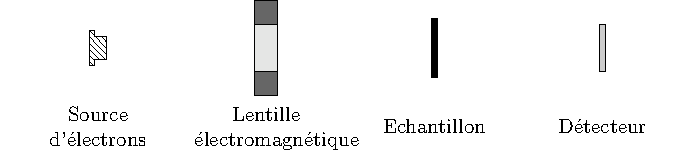
\includegraphics[]{img/chapitre1/figure1/subfig-a/electronic-legend.pdf}
       	}\\
       	\subfigure[Le microscope \gls{tem}]{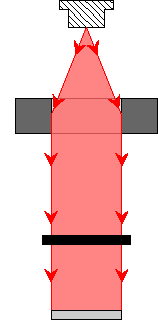
\includegraphics[]{img/chapitre1/figure1/subfig-b/electronic-tem.pdf}}
       	\hspace*{2cm}
       	%
       	\subfigure[Le microscope \gls{stem}]{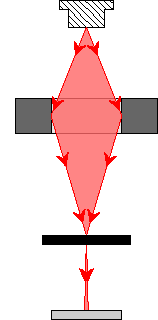
\includegraphics[]{img/chapitre1/figure1/subfig-c/electronic-stem.pdf}}
       	\hspace*{2cm}
       	%
       	\subfigure[Le microscope \gls{sem}]{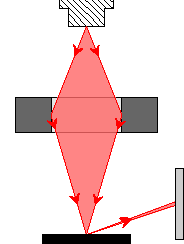
\includegraphics[]{img/chapitre1/figure1/subfig-d/electronic-sem.pdf}}
       	%
           \vspace{1em}
       	\caption{Schéma de principe des différents types de microscopie électronique.%
               \protect\label{fig-chap2-micros-electron}}
   \end{figure*}

    Les microscopes \gls{stem} et \gls{sem} se différencient du \gls{tem} puisque le faisceau balaye l'échantillon ligne par ligne au lieu de l'illuminer entièrement. Il en résulte que ces premiers sont destinés principalement à la \emph{spectroscopie}, \ie{} à l'acquisition d'un spectre pour chaque position spatiale. Les données peuvent alors être représentées comme un cube ayant deux dimensions spatiales et une dimension spectrale. Les applications classiques de ces systèmes sont la détection et cartographie d'éléments chimiques présents dans l'échantillon (\cf{} \cref{sec-exploitation-eels}). Le \gls{tem} est davantage utilisé en \emph{imagerie} pour représenter l'échantillon sans analyse chimique possible.

    La suite de ce manuscrit se focalisera sur la microscopie \gls{stem} qui est le centre de notre étude. C'est pourquoi le principe physique de la microscopie en transmission est évoqué à la \cref{subsec-principe-physique-tem} et les modalités d'acquisition classiques sont présentées à la \cref{subsec-modalitees-stem}. A cette fin, un schéma plus détaillé de ce système et de ses modalités d'acquisition est donné à la \cref{fig-chap2-stem-detail}. Enfin, le contenu technique de ce chapitre s'inspire des livre de Egerton~\cite{egerton2011electron} et de Colliex~\cite{colliex1998microscopie} et nous renvoyons les lecteurs curieux à ces ouvrages pour de plus amples informations.

    \begin{figure*}[htbp]
    	\centering
    	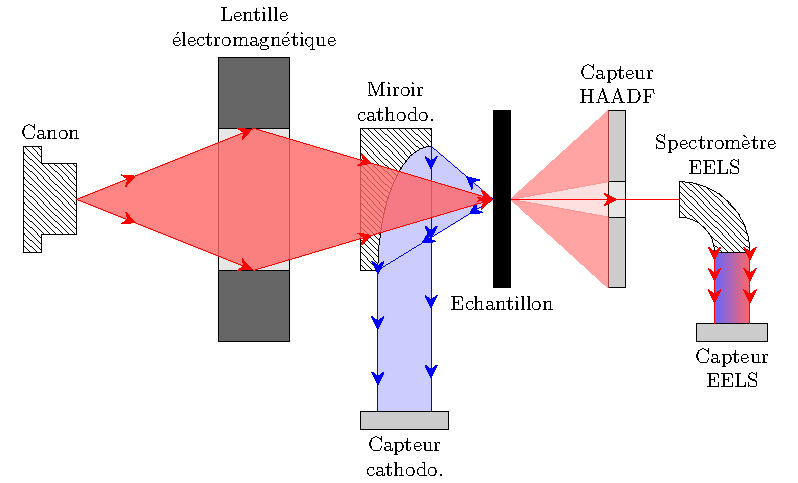
\includegraphics[]{img/chapitre1/figure2/stem-detail.pdf}
    	\caption{Un schéma de principe détaillé du \gls{stem}.
        	\protect\label{fig-chap2-stem-detail}}
    \end{figure*}

    \subsection{Principe de la microscopie en transmission}\label{subsec-principe-physique-tem}

    La microscopie en transmission étudie les interactions physiques entre un faisceau d'électron et la matière qu'il traverse. Pour ce faire, un canon fournit une certaine énergie cinétique à un faisceau d'électrons, celui-ci est alors focalisé en un point de l'échantillon à l'aide de lentilles électromagnétiques. Afin que ce faisceau \emph{traverse} l'échantillon, plusieurs conditions doivent être réunies :
    \begin{enumerate}[label=(\alph*)]
    	\item l'énergie cinétique des électrons doit être suffisante (typiquement 100keV, soit environ 2/3 de la vitesse de la lumière),
    	\item l'échantillon doit être suffisamment fin (typiquement 100nm pour un faisceau de 100keV).
    \end{enumerate}
    Dans ces conditions, les électrons traversent l'échantillon sans subir d'absorption ni de réflexion notoire. A noter qu'il est nécessaire de faire le vide dans le corps du microscope afin d'éviter toute collision entre le faisceau et les molécules d'air. Dès lors, deux types d'interactions électron-atome vont avoir lieu \emph{au sein de l'échantillon}, schématisées aux figures~\ref{fig-chap2-interactions-a} et \ref{fig-chap2-interactions-b}.

    Tout d'abord, l'électron incident interagit avec le noyau de l'atome fortement chargé par une attraction électrostatique d'autant plus intense que celui-ci s'approche du noyau, comme le montre la figure~\ref{fig-chap2-interactions-a}. Cette interaction est appelée diffusion élastique puisqu'il n'y a pas de perte d'énergie cinétique. Cela dit, la majorité des électrons traversent l'atome suffisamment loin du noyau pour être peu déviés et la déviation angulaire associée est de l'ordre du demi-degré (10\;mrad).
    
    D'autre part, l'électron incident traversant le nuage électronique peut interagir avec les électrons le constituant et leur communique de l'énergie, c'est-à-dire dans le modèle atomique les faire passer d'un niveau à un autre ou même les expulser complètement de façon à transformer l'atome initialement neutre en ion. La perte  d'énergie subie par l'électron incident est ainsi gagnée par l'électron de la cible, comme montré sur les figures~\ref{fig-chap2-interactions-b} et \ref{fig-chap2-interactions-c}. Ce type d'interaction mettant en jeu un transfert d'énergie est appelé \emph{diffusion inélastique}. La déviation angulaire est en général sensiblement plus faible que dans le cas de la diffusion élastique et les électrons concernés sont concentrés dans un domaine angulaire restreint (de l'ordre de 0.1 à 1\;mrad).
    
    Pour résumer, les électrons traversant l'échantillon peuvent être déviés de leur trajectoire par diffusion élastique ou inélastique et une partie d'entre eux ont perdu de l'énergie cinétique par diffusion inélastique. Les modalités d'acquisition du \gls{stem} se basent sur la détection de ces deux effets.

    \begin{figure}
    	\centering
    	\subfigure[Diffusion élastique]{
    \begin{tikzpicture}[scale=0.4]
        \clip (-2.6, -5) rectangle (2.5, 5);
        \coordinate (O) at (0, 0);
        \coordinate (A) at (0.4, 4);
        \coordinate (B) at (1.9, 4);

        % Circles
        \draw (O) circle (1cm);
        \draw (O) circle (2cm);

        % Central atom
        \fill[black] (O) circle (0.1cm);

        % Atoms on layers # 1
        \fill[black] (0:1) circle (0.1cm);
        \fill[black] (180:1) circle (0.1cm);

        % Atoms on layers # 2
        \fill[black] (45:2) circle (0.1cm);
        \fill[black] (90+45:2) circle (0.1cm);
        \fill[black] (180+45:2) circle (0.1cm);
        \fill[black] (270+45:2) circle (0.1cm);

        % Incident atoms
        \fill[black] (A) circle (0.1cm);
        \fill[black] (B) circle (0.1cm);

        \draw[->, thick ] (A) -- (0.4, 0) arc (0:-140:0.4) -- ++ (140:3);
        \draw[->, thick, rounded corners=1cm ] (B) -- ++(0, -4.5) -- (-2.5, -3);

    \end{tikzpicture}
    \label{fig-chap2-interactions-a}
}\quad
\subfigure[Diffusion inélastique]{\small
    \begin{tikzpicture}[scale=0.4]
        \clip (-3.25, -5) rectangle (3.25, 5);

        \coordinate (O) at (0, 0);
        \coordinate (A) at (1.4, 4);

        % Circles
        \draw (O) circle (1cm);
        \draw (O) circle (2cm);

        % Central atom
        \fill[black] (O) circle (0.1cm);

        % Atoms on layers # 1
        \fill[black] (0:1) circle (0.1cm);
        \fill[black] (180:1) circle (0.1cm);

        % Atoms on layers # 2
        \filldraw [draw=black, fill=white] (45:2) circle (0.1cm);
        \fill[black] (90+45:2) circle (0.1cm);
        \fill[black] (180+45:2) circle (0.1cm);
        \fill[black] (270+45:2) circle (0.1cm);

        % Layer # 3
        \fill [black!15, even odd rule] (O) circle (3.25cm) circle (2.75cm);
        \draw [densely dashed] (O) circle (3cm);

        % Incident atoms
        \fill[black] (A) circle (0.1cm);
        \draw (A) node [right] {$E_0$};
        \draw[->, thick, rounded corners=1cm ] (A) -- ++(0, -2.55) -- (-1.5, -3.5) node [below] {$E_0-\Delta E$};

        % Other atom and arrows
        \fill [black] (45:3) circle (0.1cm);
        \draw [->, rotate=45] (2.2, 0.1) -- ++ (0.6, 0);
        \draw [<-, dashed, rotate=45] (2.2,- 0.1) -- ++ (0.6, 0);

    \end{tikzpicture}
    \label{fig-chap2-interactions-b}
}\quad
\subfigure[Transition énergétique en diffusion inélastique]{\small
    \begin{tikzpicture}[scale=0.4]
        %\clip (-3.25, -4) rectangle (3.25, 4);

        % horiz. lines
        \draw (0, 1) node [left] {$E_{\text{1s\textsuperscript{2}}}$} -- (5, 1) node [right] {1s\textsuperscript{2}};
        \draw (0, 3) node [left] {$E_{\text{2s\textsuperscript{2}}}$} -- (5, 3) node [right] {2s\textsuperscript{2}};
        \draw (0, 4) node [left] {$E_{\text{2p\textsuperscript{6}}}$} -- (5, 4) node [right] {2p\textsuperscript{6}};

        % Valance band
        \fill [black!15] (0, 6) -- (5, 6) -- (5, 8) -- (0, 8) -- cycle;
        \draw (0, 6) -- (5, 6);
        \draw [thick] (0, 8) node [left] {$E_F$} -- (5, 8);
        \draw (5, 7) node [right] {BV};

        % Left axis
        \draw [->] (0, 0) -- (0, 10) node[above] {$E$};

        % Atoms
        \foreach \n in {1, 1.5}{\fill [black] (\n, 1) circle (0.1cm);}
        \foreach \n in {1, 1.5}{\fill [black] (\n, 3) circle (0.1cm);}
        \foreach \n in {1, 1.5, ..., 3}{\fill [black] (\n, 4) circle (0.1cm);}

        % Moved atom
        \fill [draw=black, fill=white] (3.5, 4) circle (0.1cm);
        \draw [->] (3.5, 4) -- (3.5, 7) node [left] {$\Delta E$};

    \end{tikzpicture}
    \label{fig-chap2-interactions-c}
}

        \vspace{1em}
    	\caption{Une représentation classique de la diffusion électronique inspirée de~\cite{egerton2011electron} et de \cite{colliex1998microscopie}.
        \subref{fig-chap2-interactions-a} Diffusion élastique : l'électron incident est dévié par interaction électrostatique avec le noyau. 
        \subref{fig-chap2-interactions-b} Diffusion inélastique : l'électron incident perd de l'énergie cinétique en faveur d'un électron du nuage atomique.
        \subref{fig-chap2-interactions-c} Représentation des niveaux d'énergie de l'atome. La diffusion inélastique permet à l'un des électrons du nuage électronique de passer dans un état d'énergie supérieur, en bande de valence ou au-delà.  %  
            \protect\label{fig-chap2-interactions}}
    \end{figure}


    \subsection{Les modalités d'acquisition en microscopie \glsentryshort{stem}}\label{subsec-modalitees-stem}

    Le \gls{stem} permet entre autre trois modalités d'acquisition : la cathodoluminescence, l'acquisition fond noir angulaire à grand angle (ou encore \gls{haadf}) et la spectroscopie par perte d'énergie (ou encore \gls{eels}). La \cref{fig-chap2-stem-detail} sert de support pour situer les capteurs correspondant au sein du \gls{stem}.

    \paragraph*{Cathodoluminescence.} Pour certains échantillons, le faisceau incident produit un phénomène de fluorescence dépendant de la nature de l'échantillon et de ses défauts. La technique consistant à acquérir ce signal et à l'étudier s'appelle \emph{la cathodoluminescence}. Le flux lumineux est recueilli à l'aide d'un miroir situé en amont de l'échantillon puis envoyé vers un spectromètre qui procède à l'analyse.

    \paragraph{\gls{haadf}.} Le faisceau incident se situe dans l'axe optique de l'appareil et une grande partie des électrons traversent l'échantillon en demeurant dans cet axe, la diffusion élastique est alors négligeable. Néanmoins, une partie des électrons sont significativement déviés de l'axe optique en sortie.  Un capteur annulaire placé en aval de l'échantillon capte ces électrons et délivre un signal proportionnel. Cette technique appelée \gls{haadf} permet de fournir une image 2D de l'échantillon. Un exemple d'acquisition \gls{haadf} est fourni à la \cref{fig-chap2-haadf-ex}.

    \begin{figure}%[htbp]
    	\centering
    	\subfigure[\label{fig-chap2-haadf-ex-a}Acquisition basse-résolution]%
            {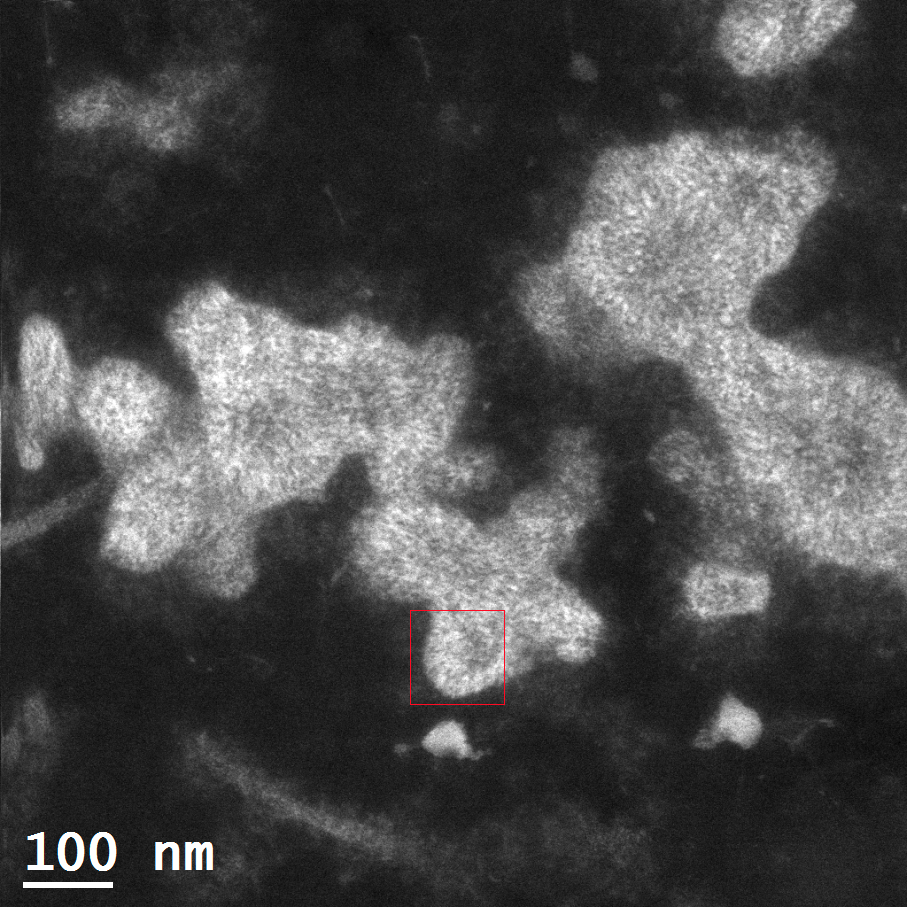
\includegraphics[height=0.25\textwidth]{img/chapitre1/figure4/haadf-LR.png}}
        \hspace{1em}
        \subfigure[\label{fig-chap2-haadf-ex-b}Acquisition haute-résolution]%
            {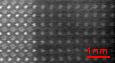
\includegraphics[height=0.25\textwidth]{img/chapitre1/figure4/haadf-HR-sc.png}}
     	%
        \caption{\protect\label{fig-chap2-haadf-ex}Exemples d'acquisitions \gls{haadf}. L'acquisition basse-résolution~\protect\subref{fig-chap2-haadf-ex-a} est de taille micrométrique  tandis que l'acquisition haute-résolution~\protect\subref{fig-chap2-haadf-ex-b} est de taille nanométrique.}
     \end{figure}


    \paragraph*{\gls{eels}.} Comme expliqué précédemment, certains électrons traversant l'échantillon  perdent une partie de leur énergie initiale par diffusion inélastique. Afin de détecter ces pertes, le faisceau demeuré dans l'axe optique frappe un spectromètre séparant les électrons en fonction de leur énergie. Une caméra CCD permet de compter, pour chaque position sur l'échantillon, la quantité d'électrons ayant conservé une énergie donnée. \`A chaque position spatiale correspond alors un spectre de perte d'énergie, les images \gls{eels} sont d'ailleurs également appelées \emph{spectre-image}. La microscopie \gls{eels} constitue le centre de cette étude, c'est pourquoi nous allons détailler ces données et leurs propriétés dans la section suivante.


    \section{Propriétés des données \glsentryshort{eels}}\label{sec-prop-eels}

    \begin{figure}[t]
        \centering
        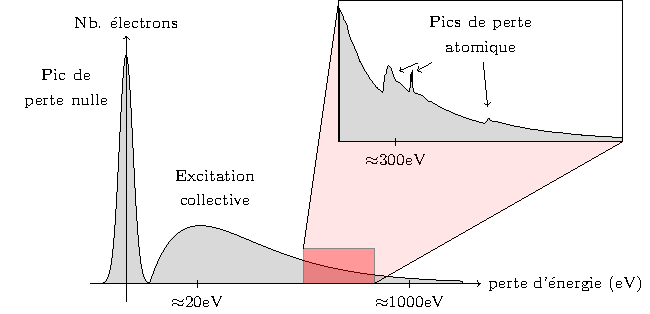
\includegraphics[]{img/chapitre1/figure5/eels-spectrum-shape.pdf}
        \caption{Représentation d'un spectre \gls{eels}.
            \protect\label{fig-chap2-eels-spectrum-shape}}
    \end{figure}

    \subsection{Caractéristiques spectrales} La forme générique d'un spectre \gls{eels} est représentée à la \cref{fig-chap2-eels-spectrum-shape} et affiche le nombre d'électrons ayant traversé l'échantillon en fonction de l'énergie perdue après la traversée (on parle de \emph{canal} pour désigner l'indice associé à une perte d'énergie). Il se compose de trois parties :
    \begin{itemize}
    	\item un pic de perte nulle qui correspond à l'ensemble des électrons ayant traversé l'échantillon sans interagir avec lui, et donc sans avoir perdu d'énergie,
    	\item un pic plus étalé correspondant à une excitation collective de la bande de valence,
    	\item une zone d'intérêt où un ensemble de pics caractéristiques (appelés \emph{seuils}) émergent du fond décroissant.
    \end{itemize}
    \emph{L'information utile est portée par la position, la forme et l'amplitude des seuils}. En effet, la position d'un seuil permet de déterminer l'élément présent dans l'échantillon tandis que son amplitude nous renseigne sur son abondance pour chaque position spatiale. Enfin, la forme du seuil peut varier suivant la configuration électronique de l'élément étudié.
    %
    \`A titre d'exemple, les seuils généralement rencontrés dans nos données se situent à des pertes d'énergie de l'ordre de \np{500} à \np[eV]{1000} (pour rappel, une énergie typique en amont de l'échantillon est \np[keV]{100}).
    %
    Des exemples réels de spectres sont donnés à la \cref{fig-chap2-eels-real-spectra-figure}.


    \begin{normalfigure*}[p]
        \centering
        \subfigure[La position des spectres]{
            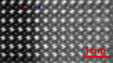
\includegraphics[width=0.3\textwidth]{img/chapitre1/figure6/eels_spectra_haadf-sc.png}
            \label{fig-chapitre2-real-eels-haadf}
        }\\
        \subfigure[Les spectres pour les trois positions]{
            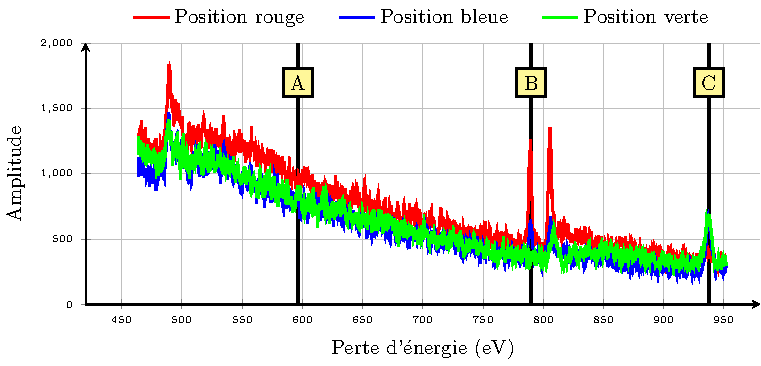
\includegraphics[]{img/chapitre1/figure6/eels_spectra.pdf}
            \label{fig-chapitre2-real-eels-spectra}
        }\\
        %
        \subfigure[Bande A]{% $\mathrm{O-K}$
            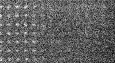
\includegraphics[width=0.3\textwidth]{img/chapitre1/figure6/eels_spectra_band_410.png}
            \label{fig-chapitre2-real-eels-bandA}
        }
        \hspace*{0.5cm}
        %
        \subfigure[Bande B ($\mathrm{La-M}_{4, 5}$)]{
            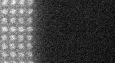
\includegraphics[width=0.3\textwidth]{img/chapitre1/figure6/eels_spectra_band_1001.png}
            \label{fig-chapitre2-real-eels-bandB}
        }
        \hspace*{0.5cm}
        %
        \subfigure[Bande C ($\mathrm{Nd-M}_{4, 5}$)]{
            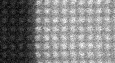
\includegraphics[width=0.3\textwidth]{img/chapitre1/figure6/eels_spectra_band_1465.png}
            \label{fig-chapitre2-real-eels-bandC}
        }

        \caption{Exemple réel de spectre-image \gls{eels}. La figure~\protect\subref{fig-chapitre2-real-eels-haadf} représente l'image \gls{haadf} de l'acquisition et trois positions en rouge, bleu et vert. Les spectres acquis en ces trois positions sont représentés à la figure~\protect\subref{fig-chapitre2-real-eels-spectra}. Enfin, les images à trois niveaux de perte d'énergie (notées A, B et C sur la figure~\subref{fig-chapitre2-real-eels-spectra}) sont représentées aux figures~\subref{fig-chapitre2-real-eels-bandA} à \subref{fig-chapitre2-real-eels-bandC}. Les bandes B et C correspondent respectivement aux signatures $\mathrm{La-M}_{4, 5}$ et $\mathrm{Nd-M}_{4, 5}$ tandis que la bande A ne correspond à aucune signature.
            \protect\label{fig-chap2-eels-real-spectra-figure}}
    \end{normalfigure*}

    \begin{figure*}[]
        \centering
        \subfigure[\label{fig-seuil-a}]{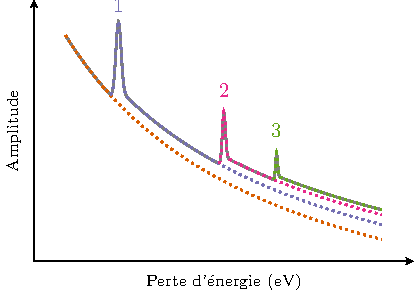
\includegraphics[]{img/chapitre1/figure6-bis/seuils.pdf}}
        \hspace{1em}
        \subfigure[\label{fig-seuil-b}]{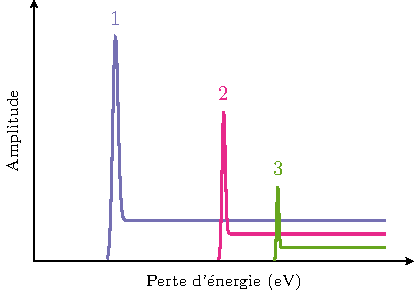
\includegraphics[]{img/chapitre1/figure6-bis/seuils-2.pdf}}
        \caption{Visualisation des effets des seuils successifs sur le spectre. La figure~\subref{fig-seuil-a} représente un spectre constitué de trois seuils. La figure~\subref{fig-seuil-b} représente les effets isolés de chacun des trois seuils. 
            \protect\label{fig-decroissance-spectre}}
    \end{figure*}

    La forme d'un seuil ne se limite pas au seul pic pour des raisons physiques, mais elle se poursuit au-delà puisque l'électron éjecté par diffusion inélastique peut avoir tout un continuum d'énergie au-delà de l'énergie de Fermi. Plus précisément, la forme du seuil varie en fonction des atomes présents au voisinage de l'élément d'intérêt, on parle de \emph{structure fine}.
    
    Le spectre acquis se décompose en un fond continu représentant l'ensemble des contributions des seuils antérieurs et d'autres phénomènes physiques, généralement modélisé par une exponentielle décroissante, et en un ensemble de seuils d'intérêt situés dans la fenêtre d'observation. La \cref{fig-decroissance-spectre} illustre cela. Cette décomposition est à la base des techniques de cartographie que l'on décrira en \cref{sec-exploitation-eels}.
    

    \subsection{Caractéristiques spatiales} En microscopie, comme pour beaucoup de systèmes d'imagerie, la caractéristique principale est le pouvoir séparateur de l'instrument, aussi appelé résolution. En microscopie \gls{stem}, celle-ci est principalement limitée par la taille de la sonde électronique (typiquement 1~nm) et par les aberrations sphériques (un correcteur permet de descendre à 0.1~nm). D'autre part, la résolution, telle qu'entendue en traitement du signal\footnote{La résolution de l'image correspond au nombre de pixels par unité de longueur. Pour éviter toute ambiguïté, on désignera par la suite la résolution de l'instrument par le terme \guillemets{pouvoir séparateur}, plus explicite.}, est choisie par l'expérimentateur en fonction de la distance parcourue par la sonde entre deux acquisitions. Cependant, en imagerie \gls{eels}, la taille de l'image excède rarement $10^5$ pixels pour limiter le temps d'acquisition et éviter de détériorer l'échantillon (comme décrit à la section~\ref{sec-ech-sensibles}). Par conséquent, deux situations apparaissent~:
    \begin{itemize}
        \item l'expérimentateur étudie des structures spatiales étendues (typiquement 100~nm) et est obligé de limiter la résolution, les images sont alors basse-résolution (\cf{} \cref{fig-chap2-haadf-ex-a}),
        \item l'expérimentateur étudie des réseaux atomiques très localisés (typiquement quelques nanomètres) et la résolution est limitée par l'instrument, les images sont alors haute-résolution (\cf{} \cref{fig-chap2-haadf-ex-b}).
    \end{itemize}
    Enfin, il faut noter que la structure spatiale est plus ou moins visible selon le canal considéré dans l'image \gls{eels}. Par exemple, la \cref{fig-chapitre2-real-eels-bandA} correspond à une zone du spectre où aucun contraste n'apparaît clairement, il en résulte que l'image est fortement bruitée. A contrario, les images situées sur des seuils particuliers du spectre sont moins bruitées et mettent clairement en évidence la position des éléments concernés, comme pour les \cref{fig-chapitre2-real-eels-bandB,fig-chapitre2-real-eels-bandC}.  La cartographie des éléments présents dans l'échantillon requiert des méthodes particulières afin de soustraire la contribution du fond continu, comme nous le verrons à la \cref{sec-exploitation-eels}.

    \subsection{Nature du bruit}\label{sec-nature-bruit}
    
    Les sources de bruit sont multiples en imagerie \gls{eels}, mais le type de bruit le plus attendu est poissonien. Cela modélise tant la probabilité qu'un électron du faisceau subisse un certain nombre de diffusions inélastique au sein de l'échantillon~\cite[Section~4.1.1]{egerton2011electron} que la probabilité qu'une cellule du capteur reçoive un électron sur une période donnée. \`A cela s'ajoute un bruit gaussien dû à l'électronique d'acquisition.
    %
    En pratique, la nature du bruit est expérimentalement complexe à déterminer.
    %
    \`A ce bruit d'acquisition vient s'ajouter les instabilités spatiales de l'échantillon : celui-ci dérive au cours de l'acquisition à cause de variations de température et de mouvements d'air~\cite{zobelli2019spatial}. Ces déplacements ne sont pas visibles pour des images basse-résolution mais deviennent critiques à des échelles atomiques puisque le réseau atomique initialement aligné peu apparaître déformé\footnote{Ce n'est pas systématiquement le cas puisque l'expérimentateur limite la dérive, comme expliqué à la section~\ref{sec-ech-sensibles}.}, comme le montre la \cref{fig-drift}.
    %


    \subsection{ACP et redondance spectrale}\label{sec-acp-redondance}

    Le spectre-image \gls{eels} comporte généralement une grande quantité de pixels $\gls{P}\approx 10^4$ et de canaux $\gls{M}\approx 10^3$, conduisant à un nombre de coefficients de l'ordre de $10^7$. La très grande dimension de ces données complique toute analyse directe de l'image et l'on cherche à simplifier l'étude \emph{en réduisant la taille des données tout en conservant le maximum d'information intrinsèque}. Un outil fondamental permettant cela est l'\gls{acp} qui réduit la dimension des données en extrayant les composantes les plus informatives. Cette technique présentée dans cette section s'appuie sur une propriété essentielle des données \gls{eels} : la redondance spectrale.

    \begin{marginfigure}
        \centering
        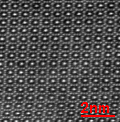
\includegraphics[width=0.7\textwidth]{img/chapitre1/figure7/drift-sc.png}
        \caption{Un exemple de défaut en haute résolution : la dérive de l'échantillon. L'échantillonnage se fait ligne par ligne. On observe que, dans ce cas, l'échantillon dérivait sur la gauche, puis vers le haut. Il en résulte une déformation notable et préjudiciable du réseau atomique.
            \protect\label{fig-drift}}
    \end{marginfigure}

    \paragraph{Présentation générale de l'ACP.} L'\gls{acp} est une technique utilisée en analyse multivariée qui consiste à transformer $M$ variables corrélées entre elles en autant de nouvelles variables décorrélées les unes des autres. Pour cela, la transformation estime successivement les axes dans $\mathbb{R}^M$ maximisant la variance des variables projetées sur cet axe (à chaque nouvel axe estimé, sa contribution est soustraite aux données avant d'estimer l'axe suivant). Ces axes successifs sont appelés les \emph{composantes principales des données}.
    Plus précisément, cette transformation décrite plus en détail dans~\cite{jolliffe2002springer} requiert le spectre-image \gls{Y} de taille \taille{M}{P} où chaque colonne correspond à un spectre \gls{eels} et où chaque ligne est une image pour un canal donné. Notons que la moyenne empirique des spectres est supposée être soustraite de sorte que les données $\tilde{\mathbf{Y}}=\gls{Y}-\frac{1}{P}\sum_p\mathbf{Y}_p$ soient centrées.
    %
    Ainsi, l'ACP transforme l'image $\tilde{\gls{Y}}$ dont les spectres sont possiblement corrélés en les données transformées $\mathbf{S} = [\mathbf{s}_1,\dots,\mathbf{s}_M]^T$ (aussi appelées \emph{variables de représentation}) décorrélées de telle sorte que
    \begin{equation}\label{eq-decomposition-acp}
    \mathbf{S}_\mathbf{Y} = \gls{H}^T\tilde{\gls{Y}}
    \end{equation}
    où $\gls{H} = [\mathbf{h}_1,\dots,\mathbf{h}_M]$ est une matrice orthogonale de taille \taille{M}{M} contenant les composantes principales de \gls{Y}. Remarquons que l'orthogonalité de \gls{H} dans la transformation~\eqref{eq-decomposition-acp} permet de considérer l'\gls{acp} comme un changement de base dans $\mathbb{R}^M$ dont les vecteurs $\mathbf{h}_1,\dots,\mathbf{h}_M$ forment la nouvelle base. 
    %
    En pratique, la matrice $\gls{H}$ est obtenue en diagonalisant la matrice de variance-covariance $\tilde{\mathbf{C}} = \frac{1}{p-1}\tilde{\gls{Y}}\tilde{\gls{Y}}^T$. Les vecteurs propres constituent la matrice $\gls{H}$ tandis que chaque valeur propre $\gls{d}_m$ correspond à la variance de la représentation $\mathbf{s}_m$ pour une composante principale $\mathbf{h}_m$ donnée. On désigne ainsi la valeur propre $\gls{d}_m$ comme la puissance associée à la composante principale $\mathbf{h}_m$ et les colonnes de \gls{H} sont triées par puissance décroissante. 
    %
    Enfin, précisons que l'estimation des composantes principales est d'autant meilleure que la matrice de covariance est correctement estimée, à savoir $P\gg M$.

    \paragraph{Matrice de covariance ou matrice de corrélation ?} Dans le paragraphe précédent, la moyenne empirique $\boldsymbol\mu = [\mu_1,\dots,\mu_M]^T$ a été soustraite aux données afin d'obtenir les données centrées
    \begin{equation}
     \tilde{\mathbf{Y}} =
        \begin{pmatrix}
        \mathbf{Y}_{1 1} - \mu_1&\mathbf{Y}_{1 2} - \mu_1&\cdots&\mathbf{Y}_{1 P} - \mu_1\\
        \mathbf{Y}_{2 1} - \mu_2&\mathbf{Y}_{2 2} - \mu_2&\cdots&\mathbf{Y}_{2 P} - \mu_2\\
        \vdots&\vdots&\ddots&\vdots\\
        \mathbf{Y}_{M 1} - \mu_M&\mathbf{Y}_{M 2} - \mu_M&\cdots&\mathbf{Y}_{M P} - \mu_M
        \end{pmatrix}.
    \end{equation}
    La matrice de covariance $\tilde{\mathbf{C}} = \frac{1}{p-1}\tilde{\gls{Y}}\tilde{\gls{Y}}^T$ est ensuite calculée afin d'extraire les composantes principales. Cette méthode a un défaut majeur : si un canal d'indice $m_0\in\llbracket 1,M\rrbracket$ correspond à un seuil d'amplitude très supérieure aux amplitudes des autres seuils, alors celui-ci va \guillemets{tirer} les résultats de l'ACP vers lui au détriment des autres caractéristiques~\cite[Section~3.3]{jolliffe2002springer}.
    %
    Dans ce genre de cas, l'alternative consiste estimer les écarts-types empiriques $\boldsymbol\sigma=[\sigma_1,\dots,\sigma_M]^T$, puis à réduire les données
    \begin{equation}
    \bar{\mathbf{Y}} =
    \begin{pmatrix}
    \frac{\mathbf{Y}_{1 1} - \mu_1}{\sigma_1}&
    \frac{\mathbf{Y}_{1 2} - \mu_1}{\sigma_1}&
    \cdots&
    \frac{\mathbf{Y}_{1 P} - \mu_1}{\sigma_1}\\
    %
    \frac{\mathbf{Y}_{2 1} - \mu_2}{\sigma_2}&
    \frac{\mathbf{Y}_{2 2} - \mu_2}{\sigma_2}&
    \cdots&
    \frac{\mathbf{Y}_{2 P} - \mu_2}{\sigma_2}\\
    %
    \vdots&\vdots&\ddots&\vdots\\
    %
    \frac{\mathbf{Y}_{M 1} - \mu_M}{\sigma_M}&
    \frac{\mathbf{Y}_{M 2} - \mu_M}{\sigma_M}&
    \cdots&
    \frac{\mathbf{Y}_{M P} - \mu_M}{\sigma_M}
    \end{pmatrix}.
    \end{equation}
    La matrice de \emph{corrélation} $\bar{\mathbf{C}} = \frac{1}{p-1}\bar{\gls{Y}}\bar{\gls{Y}}^T$ est ensuite diagonalisée afin d'extraire les composantes principales. %
    %
    Si cette technique permet de prévenir le défaut lié à la matrice de covariance, elle présente elle-même un inconvénient puisqu'elle est plus apte à capturer des seuils apparentés au bruit.
    %
    Ces aspects sont détaillés et discutés a l'annexe~\ref{abstr-pca-corr-cov}. Dans le cadre de cette étude, la matrice de covariance sera utilisée.


    \paragraph{L'ACP en vue de réduire la dimension.} L'ACP est d'autant plus performante à réduire la dimension des données que celles-ci sont corrélées. En effet, si les observations sont fortement corrélées, on observe que les variances des variables de représentation associées aux premières composantes principales sont particulièrement élevées par rapport aux variances des variables de représentation associées aux dernières composantes principales.
    %
    Ainsi, l'on observe généralement un changement de comportement à un indice $\gls{R}\ll M$ d'autant plus faible que les données sont corrélées, ou à défaut de variation brutale de la courbe des puissances, on choisit l'indice \gls{R} tel que les \gls{R} premières composantes principales regroupent une fraction élevée de la puissance totale.
    %
    Dans ce cas, il est possible d'approximer les données \gls{Y} par une matrice $\hat{\gls{Y}}_{1:R}$ en projetant les données sur le sous-espace de dimension \gls{R} généré par les \gls{R} premières composantes principales, puis en les rétro-projetant dans $\mathbb{R}^M$. Ainsi, l'approximation à l'ordre \gls{R} s'écrit
    \begin{equation}
    \hat{\gls{Y}}_{1:R} = \gls{H}_{1:R}\gls{H}_{1:R}^T\gls{Y}
    \end{equation}
    où $\gls{H}_{1:R}$ correspond aux $R$ premières colonnes de $\gls{H}$. Cette approximation est d'autant plus fidèle que les données sont fortement corrélées, comme le montre la \cref{fig-pca-data-corr}.

    \begin{figure*}[]
        \centering
        \subfigure[\label{fig-pca-data-corr-a}$\mathrm{corr} = 0$]{
            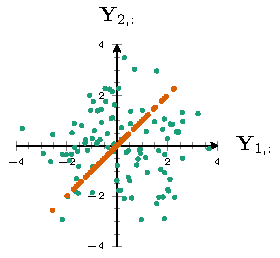
\includegraphics{img/chapitre1/figure15/pca-corr-1.pdf}}
        \subfigure[\label{fig-pca-data-corr-b}$\mathrm{corr} = 0.95$]{
            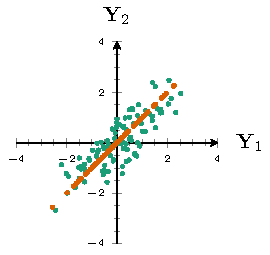
\includegraphics{img/chapitre1/figure15/pca-corr-2.pdf}}
        \subfigure[\label{fig-pca-data-corr-c}$\mathrm{corr} = 99$]{
            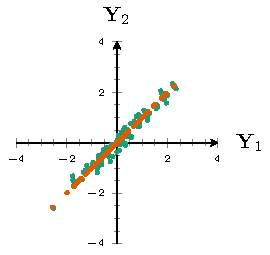
\includegraphics{img/chapitre1/figure15/pca-corr-3.pdf}}
        \caption{Trois exemples de nuages de points avec $M=2$ et $P=100$ (en vert) et leur approximation au 1er ordre (en orange). Les coefficients de corrélation valent respectivement 0, 0.95 et 0.99 pour les figures~\protect\subref{fig-pca-data-corr-a}, \protect\subref{fig-pca-data-corr-b} et \protect\subref{fig-pca-data-corr-c}. L'approximation du premier ordre est d'autant meilleure que les données sont corrélées. En particulier, ne conserver que la première composante principale est suffisant pour la figure~\protect\subref{fig-pca-data-corr-c}.
            \protect\label{fig-pca-data-corr}}
    \end{figure*}

    \paragraph{Application aux données EELS.} L’imagerie hyperspectrale est une technique combinant l’imagerie et la spectroscopie où chaque pixel de l'image est caractérisé par un spectre électromagnétique. Ces images spectroscopiques sont utilisés dans de nombreux domaines incluant la télédétection~\cite{schaepman2009earth}, la planétologie~\cite{smith1985quantitative}, le contrôle des aliments~\cite{gowen2007hyperspectral} et l'ingénierie biomédicale~\cite{akbari2010detection}. Si les spectres \gls{eels} ne sont pas de nature électromagnétiques, les spectre-images sont néanmoins un cas particulier d'images hyperspectrales puisqu'elles partagent un très grand nombre de propriétés et de méthodes d'analyse.
    %
    La popularité de ces techniques découle d'une propriété fondamentale des données hyperspectrales~: la redondance spectrale. En effet, les spectres issus de ces images sont connus pour être fortement corrélés spectralement~\cite{dobigeon2016linear, bioucas2012hyperspectral, dobigeon2012spectral} et le paradigme du démélange (discuté en détail à la \cref{sec-demelange}) en donne une interprétation physique. Dans ce paradigme, chaque spectre acquis est supposé être le mélange de signatures spectrales élémentaires appelés \emph{endmembers} correspondant à des éléments particuliers de la scène (\eg{} de l'eau, des bâtiments ou de la végétation en télédétection).
    %
    Tout cela permet de conclure que les spectres, loin de remplir $\mathbb{R}^M$ uniformément, évoluent dans une variété de dimension $\gls{R}\ll M$. Par défaut, cette variété n'est pas plane puisque des non-linéarités interviennent dans le mélange, causés par des phénomènes physiques au niveau local. Néanmoins, une approximation linéaire peut être réalisée afin d'estimer le sous-espace de dimension réduite appelé \emph{sous-espace signal}, possiblement à l'aide d'une \gls{acp}. L'identification de ce sous-espace permet d'obtenir des variables de représentation de dimension réduite pourtant très précises, ouvrant la voie à un gain considérable en temps de calcul, en complexité et en stockage de donnée pour une qualité d'image équivalente. Comme expliqué plus haut, l'\gls{acp} réduit d'autant la dimension du spectre-image (ou encore \gls{R} est d'autant plus faible) que les données sont corrélées \ie{} que peu d'éléments élémentaires sont présent dans la scène. La \cref{fig-ACP} montre les composantes principales d'un spectre-image réel. L'évolution des puissances issues de l'\gls{acp} affichées à la \cref{fig-sub-pca-eigs} nous permet de déterminer trois comportements\footnote{Il faut noter que les puissances ont été corrigées afin de compenser l'erreur d'estimation dû au faible nombre d'observations (le nombre de pixels est du même ordre de grandeur que le nombre de canaux), comme expliqué à la \cref{subsec-3s-acp}.}.
    \begin{normalfigure*}[htbp]
        \centering
        \subfigure[Evolution des valeurs propres associées à l'\gls{acp}]{
            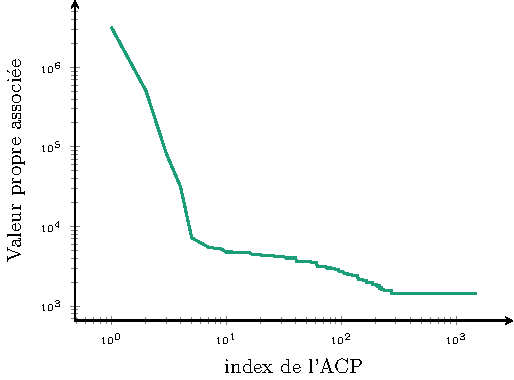
\includegraphics[]{img/chapitre1/figure9/PCA_eigs.pdf}
            \label{fig-sub-pca-eigs}}
        \\
        \subfigure[Variable de repr. \num\ 1]{\label{fig-sub-pca-comp1}
            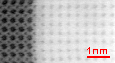
\includegraphics[width=0.28\textwidth]{img/chapitre1/figure9/PCA_map_0-sc.png}}\vspace{20pt}
        \subfigure[Variable de repr. \num\ 2]{\label{fig-sub-pca-comp2}
            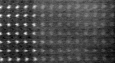
\includegraphics[width=0.28\textwidth]{img/chapitre1/figure9/PCA_map_1.png}}\vspace{20pt}
        \subfigure[Variable de repr. \num\ 3]{\label{fig-sub-pca-comp3}
            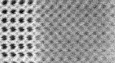
\includegraphics[width=0.28\textwidth]{img/chapitre1/figure9/PCA_map_2.png}}\\
        \subfigure[Variable de repr. \num\ 4]{\label{fig-sub-pca-comp4}
            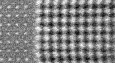
\includegraphics[width=0.28\textwidth]{img/chapitre1/figure9/PCA_map_3.png}}\vspace{20pt}
        \subfigure[Variable de repr. \num\ 5]{\label{fig-sub-pca-comp5}
            
\includegraphics[width=0.28\textwidth]{img/chapitre1/figure9/PCA_map_4.png}}\vspace{20pt}
        \subfigure[Variable de repr. \num\ 6]{\label{fig-sub-pca-comp6}
            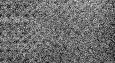
\includegraphics[width=0.28\textwidth]{img/chapitre1/figure9/PCA_map_5.png}
        }\\
        %
        \def\comp{mean}
        \subfigure[Spectre moyen]{
            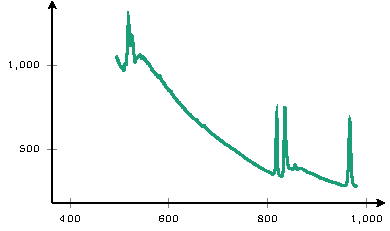
\includegraphics[]{img/chapitre1/figure9/PCA_spectra_1.pdf}
            \label{fig-sub-pca-mean}}%
        %
        \def\comp{comp0}%
        \subfigure[Première composante]{
            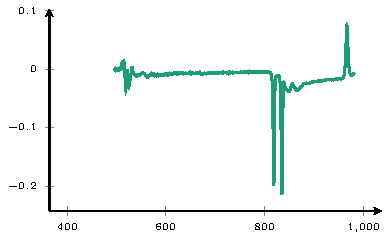
\includegraphics[]{img/chapitre1/figure9/PCA_spectra_2.pdf}
            \label{fig-sub-pca-spectrum-0}}
        %
        \caption{L'analyse par \gls{acp} de données \gls{eels}. La figure~\subref{fig-sub-pca-eigs} représente l'évolution des valeurs propres associées à l'\gls{acp}. On observe, entre autres, que seules les 5 premières composantes sont vraiment significatives. Les figures \subref{fig-sub-pca-comp1} à \subref{fig-sub-pca-comp6} représentent les variables de représentation associées aux composantes principales les plus puissantes. Le spectre moyen donné à la figure~\subref{fig-sub-pca-mean} est soustrait aux données avant d'appliquer l'\gls{acp}. Il en résulte que les spectres associés aux composantes principales sont des variations par rapport à ce spectre moyen, ce qui explique que la première composante affichée à la figure~\subref{fig-sub-pca-spectrum-0} soit parfois négative.
            \protect\label{fig-ACP}}
    \end{normalfigure*}    
    \begin{itemize}
        \item Les premières composantes de puissance très élevées correspondent à des éléments chimiques présents en forte quantité dont les projections associées (\cf{} \crefrange{fig-sub-pca-comp1}{fig-sub-pca-comp4}) renferment beaucoup d'information spatiale et peu de bruit. Le spectre associé à la première composante est lui-même très peu bruité (\cf{} \cref{fig-sub-pca-spectrum-0}).
        \item Un ensemble de composantes principales situées entre les indices 5 et 300 se démarque encore par sa puissance, bien que moins important que les premières composantes. L'évolution de leur puissance est également moins rapide. Il s'agit généralement de composants très localisés spatialement ou issus de mélanges non-linéaires. Certaines informations spatiales peuvent être encore discernées chez les projections associées aux composantes les plus puissantes, comme à la \cref{fig-sub-pca-comp5}.
        \item Les dernières composantes présentent enfin une puissance constante correspondant à la puissance estimée du bruit. Plus aucune information n'est visible ni dans le spectre associé ni dans la projection correspondante.
    \end{itemize}
    Cette observation permet généralement le débruitage des données en supprimant les composantes principales associées au bruit, comme décrit à la \cref{sec-ech-sensibles}. Malheureusement, le choix du seuil \gls{R} correspondant à la dimension du sous-espace estimé n'est pas trivial. Deux solutions seront cependant proposées: l'une basée sur l'évolution des valeurs propres à la \cref{subsec-3s-acp}, l'autre analysant le contenu spatial des images issues des projections sur les composantes principales à l'annexe~\ref{sec-spim-creation-hr}

    

    %
    \section{Cartographie par séparation de composantes spectrales}\label{sec-exploitation-eels}

    Le problème généralement rencontré lors de l'exploitation des données \gls{eels} consiste à localiser et à cartographier un ensemble de composés chimiques élémentaires présents dans l'échantillon~\cite{colliex2012stem, pennycook2011seeing, dobigeon2012spectral}.
    %
    Pour cela, nous pouvons exploiter l'information spectrale contenue aux abords du seuil associé à l'élément étudié. En effet, plus il est abondant en une position spatiale, plus l'amplitude du seuil associé est grande. En couplant l'information obtenue en chaque position, une image appelée \emph{carte d'abondance} renseignant sur sa répartition spatiale peut être générée. 
    %
    Ce problème est plus largement rencontré en imagerie hyperspectrale, comme en télédétection afin de cartographier des constituants élémentaires au sein d'une scène~\cite{lelong1998hyperspectral} (\eg{} eau, bâtiments, etc).
    %
    La technique historique classiquement utilisée en imagerie \gls{eels} analyse de manière supervisée les spectres pris indépendamment afin de quantifier un élément particulier.
    %
    A l'inverse, des approches plus récentes analysent le spectre-image dans son entièreté de manière non-supervisée afin de cartographier l'ensemble des composantes d'intérêt. 


    \subsection{Quantification par ajustement d'exponentielle}
    
    Comme expliqué à la \cref{sec-prop-eels}, un spectre \gls{eels} contient la contribution de plusieurs seuils successifs et d'un fond continu. Pour pallier ce problème, le fond décroissant et la rémanence des seuils précédents devront être soustraits avant d'intégrer le seuil d'intérêt. Pour illustrer cette méthode, considérons le spectre affiché à la \cref{fig-carto-separation-a}, correspondant à une position spatiale donnée. Une zone de régression est choisie en amont du seuil (tout en restant proche du seuil) et une régression exponentielle de la forme $y=Ax^{-r}$ est effectuée (\cf{}~\cite[Section~4.4]{egerton2011electron} pour plus de détails). La courbe estimée est alors soustraite pour obtenir un spectre corrigé propre à ce seuil, \ie{}, le seuil étudié n'est plus influencé par le fond continu. L'abondance du composé pour cette position spatiale est ensuite calculée en sommant le spectre dans une zone centrée sur le seuil d'intérêt. En effectuant cette opération pour toutes les positions spatiales, nous pouvons reconstituer la carte d'abondance de la \cref{fig-carto-separation-b}. \`A noter que les paramètres de la régression dépendent de la position spatiale.

    Afin d'effectuer la cartographie de plusieurs composantes présentes dans l'échantillon, l'expérimentateur doit alors exécuter cette opération pour tous les seuils présents dans le spectre. Cette technique est simple et une implémentation automatique est facile à mettre en \oe{}uvre dès lors que les zones de régression et d'intégration ont été définies.
    
    \begin{figure*}[t]
        \centering
        \subfigure[\label{fig-carto-separation-a}]{
            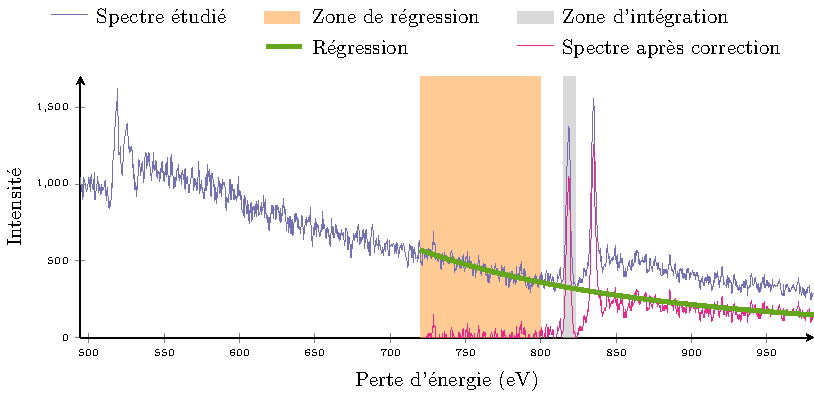
\includegraphics[]{img/chapitre1/figure11/separation.pdf}}\hspace{1em}
        \subfigure[\label{fig-carto-separation-b}]{
            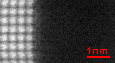
\includegraphics[width=5cm]{img/chapitre1/figure11/regression-sc.png}}
        \caption{Illustration de la méthode de cartographie par ajustement d'exponentielles spectrales. \protect\subref{fig-carto-separation-a} Régression pour une position particulière. Une régression exponentielle est effectuée sur la zone de régression, puis est soustraite au spectre pour obtenir le spectre corrigé. L'abondance est finalement calculée en intégrant le spectre autours du pic d'intérêt. \protect\subref{fig-carto-separation-b} Résultat en effectuant cette action sur tous les pixels (l'élément cartographié est $\mathrm{La-M}_{4, 5}$). A noter que les paramètres de la régression dépendent de la position spatiale.
            \protect\label{fig-carto-separation}}
    \end{figure*}
    
    Cependant, cette technique ne permet que la \emph{quantification} de l'élément à une constante près quel que soit son environnement\,; elle ne permet entre autres pas d'obtenir des proportions contrairement au démélange discuté à la section suivante. Or, la structure fine, c'est-à-dire la forme du seuil, renseigne sur l'état du composé étudié et la technique ci-dessus ne fait aucune distinction lors de la quantification. Par exemple, les travaux menés dans~\cite{dobigeon2012spectral} s'intéressent à l'état d'oxydation du bore et tentent de cartographier deux états distincts, la forme oxydée B\textsubscript{2}O\textsubscript{3} et la forme azotée BN. Dans ce cas, la technique proposée ne fait pas cette distinction.
    %
    Pour résoudre cette impasse, des techniques de cartographie non-supervisée ont été proposées ces dernières décennies afin de ne pas considérer le pic uniquement, mais l'ensemble du spectre.

    

    \subsection{Techniques de cartographie non-supervisée}\label{sec-demelange}
    
    \paragraph{Approches par ACP et ACI.} La redondance spectrale présentée à la section précédente suggère que les spectres acquis soient le résultat d'un mélange de $N_c$ spectres élémentaires $\mathbf{m}_1,\dots,\mathbf{m}_{N_c}$ appelés \emph{endmember}, correspondant aux signatures associées aux composés caractéristiques présents dans l'échantillon.
    %    
    Estimer les signatures $\mathbf{m}_k$ s'apparente à de la séparation aveugle de sources et les premières techniques non-supervisée proposées l'ont considéré d'un point de vue statistique en usant des techniques d'analyse multivariée. Dans cette perspective, l'\gls{acp} a été utilisée afin d'extraire les signatures de spectre-images \gls{eels} dans~\cite{bonnet1999extracting, bosman2006mapping, trebbia1990eels}, mais cette méthode renvoie des spectres difficiles à interpréter physiquement, à cause notamment de la contrainte d'orthogonalité inhérente à l'\gls{acp} imposée aux endmembers. L'\gls{aci} a été envisagée comme alternative afin d'analyser les données hyperspectrales issues de la télédétection~\cite{bayliss1998analyzing, chen1999independent} ou de l'imagerie \gls{stem}-\gls{eels}~\cite{delapena2011mapping, bonnet2005independent, bosman2006mapping}. Malheureusement, l'\gls{aci} repose sur l'hypothèse que les signatures spectrales comme leur abondance soient indépendantes, ce qui n'est pas le cas puisque si un élément est fortement présent, les autres le seront généralement moins. Cela compromet l'utilisation de l'\gls{aci} en démélange hyperspectral, d'autant que ni l'\gls{acp}, ni l'\gls{aci} ne permettent de contraindre l'abondance à être positive et leurs résultats demeurent en général difficile à interpréter d'un point de vue physique. Toutefois, l'ACI peut donner des résultats intéressants et rapides pour certains jeux de données et cela peut être un point de départ dans l'analyse de l'image.
    
    \paragraph{Approches par démélange.} Comme expliqué précédemment, les spectres acquis sont supposés être le résultat d'un mélange de $N_c$ spectres élémentaires\,; une hypothèse de mélange linéaire est souvent réalisée afin de simplifier l'interprétation et la résolution du problème inverse associé. Dans ce cas, le modèle direct s'écrit~\cite{dobigeon2016linear}
    \begin{align}
    &\gls{Y} = \mathbf{M}\mathbf{A}\\
    \text{tel que}\quad &\mathbf{A} \geq 0\qquad \mathbf{M} \geq 0\label{eq-positivity}\\
    &\sum_k \mathbf{A}_{kp} = 1 \quad \forall p\in\llbracket 1 , P \rrbracket \label{eq-sum-to-one}
    \end{align}
    où $\mathbf{M}=[\mathbf{m}_1,\dots,\mathbf{m}_{N_c}]$ de taille $M\times N_c$ est la matrice contenant les signatures spectrales et où $\mathbf{A} = [\mathbf{a}_1,\dots,\mathbf{a}_{N_c}]^T$ est la matrice d'abondance de taille $N_c\times P$. Chaque ligne $\mathbf{a}_c$ est une image représentant la proportion de l'endmember $\mathbf{m}_k$ au sein de l'échantillon, il s'agit de la carte d'abondance. Deux hypothèses portant sur $\mathbf{A}$ sont réalisées : l'hypothèse de positivité à l'équation~\eqref{eq-positivity} et l'hypothèse de somme à un à l'équation~\eqref{eq-sum-to-one}.
    \begin{description}
        \item[Positivité] L'abondance de l'élément ne peut être négative puisqu'il s'agit d'une proportion. Et puisque le spectre est positif, les entrées de $\mathbf{A}$ et de $\mathbf{M}$ sont donc positives.
        \item[Somme à un] La somme des abondances vaut un pour toute position spatiale. Cette hypothèse traduit le fait que les éléments de $\mathbf{A}$ soient des proportions. Cependant, pour que l'on puisse comparer les proportions d'un pixel à l'autre, il est nécessaire que la quantité de matière traversée par le faisceau soit la même sur l'ensemble de l'échantillon, sans quoi deux proportions identiques ne traduiraient pas une quantité égale de l'élément.
    \end{description}
    Une représentation géométrique du mélange linéaire est donné à la \cref{fig-melange-lineaire} pour $M=3$ et $N_c=3$. Les coordonnées des trois endmembers $\mathbf{m}_1,\mathbf{m}_2,\mathbf{m}_3$ sont représentés dans $\mathbb{R}_3$ et puisque la contrainte de somme à un est utilisée ici, l'ensemble des spectres obtenus par mélange linéaire se situent dans le plan de dimension $M-1=2$ généré par ces trois vecteurs (à condition qu'ils soient linéairement indépendants). Enfin, l'hypothèse de positivité contraint l'ensemble des spectres de \gls{Y} à évoluer dans le simplexe formé par $\mathbf{m}_1$, $\mathbf{m}_2$ et $\mathbf{m}_3$.
    \begin{figure}
        \centering
        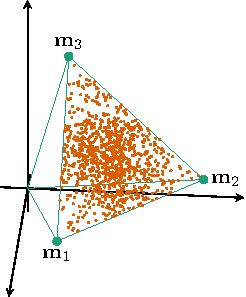
\includegraphics[]{img/chapitre1/figure17/melange_lineaire.pdf}
        \caption{Une représentation géométrique du modèle de mélange linéaire pour $M=3$ et $N_c=3$. Les spectres élémentaires sont notés $\mathbf{m}_1$, $\mathbf{m}_2$ et $\mathbf{m}_3$. La contrainte de somme à un contraint les spectres constitutifs de \gls{Y} (en orange) à évoluer dans le plan formé par ces trois vecteurs tandis que la contrainte de positivité les contraint à demeurer dans le simplexe formé par les endmembers.
            \protect\label{fig-melange-lineaire}}
    \end{figure}
    Maintenant que le modèle direct est posé, le problème inverse consiste à estimer conjointement les spectres élémentaires $(\mathbf{m}_k)_{k=1,\dots,N_c}$ ainsi que les cartes d'abondance associées. Ce problème inverse est appelé \emph{démélange hyperspectral}~\cite{bioucas2012hyperspectral, dobigeon2016linear} ou \emph{unmixing} et s'apparente à un problème de séparation aveugle de source~\cite{comon2010handbook}. Il requiert la connaissance du nombre de composantes $N_c$.
    %
    Une technique de démélange non-supervisée a pour but d'estimer les endmembers, ou de manière géométrique le simplexe dans lequel évoluent les spectres acquis et dont les endmembers constituent les sommets, et la matrice d'abondance associée\footnote{Le nombre d'endmember est lui-aussi inconnu dans la plupart des situations, mais il peut être estimé par une autre méthode a priori.}. Souvent, ce problème d'estimation est généralement non-convexe et on lui préfère une résolution sous-optimale en deux temps. D'abord, les signatures élémentaires sont déterminées à l'aide d'un algorithme d'extraction d'endmember, puis la matrice d'abondance est déterminée. Néanmoins, des méthodes bayésiennes permettent une estimation conjointe des endmembers et de des abondances basées sur un modèle statistique.

    \paragraph{Estimation des endmembers.} Les premières méthodes d'extraction d'endmember utilisées furent l'ACP et l'ACI avec les inconvénients relevés plus haut.
    % 
    Une autre approche du problème consiste à user de l'interprétation géométrique réalisée plus haut afin d'estimer les endmembers $\mathbf{m}_k$. Dans l'hypothèse où les composantes pures sont présentes dans l'échantillon, des techniques efficaces et rapides permettent de déterminer les spectres acquis correspondant aux endmembers. Par exemple, \gls{vca}~\cite{nascimento2005vertex} projette itérativement les données sur un axe orthogonal au sous-espace généré par les endmembers déjà déterminés. Le nouvel endmember correspond au point extrême de la projection et l'algorithme est itéré jusqu'à obtenir toutes les composantes. Néanmoins, l'hypothèse de pixels purs est généralement trop forte. En microscopie \gls{stem}-\gls{eels}, par exemple, à cause d'une résolution insuffisante ou d'une épaisseur d'échantillon permettant la superposition d'éléments différents, on n'acquiert pas de spectre pur. Pour relâcher cette contrainte, les techniques par minimisation de volume estiment la matrice $\mathbf{M}$ de sorte que le simplexe généré par les endmembers $\mathbf{m}_i$ soit de volume minimal tout en contenant l'ensemble des spectres acquis. Ce problème devient plus difficile à résoudre puisqu'il est non-convexe, c'est pourquoi il est initialisé à l'aide d'une autre technique comme \gls{vca}. L'algorithme \gls{sisal}~\cite{bioucas2009variable} implémente une version plus robuste en autorisant la violation de la contrainte de positivité, c'est pourquoi certains spectres estimés par SISAL peuvent être négatifs, mais cette violation est contrainte à l'aide de la fonction hinge $h$ ($h(x) = 0$ si $x \geq 0$ et $h(x)=-x$ si $x<0$). Les techniques par approche géométrique sont rapides et efficaces si l'image présente des pixels purs, autrement, ces performances sont réduites et des techniques statistiques sont à préférer.
    
    \paragraph{Estimation des abondances.} Une fois l'extraction des endmembers réalisée, on doit estimer les abondances.  Cela consiste à déterminer le sous-ensemble optimal de signatures spectrales ainsi que les proportions associées pouvant décrire chaque pixel mélangé de l'échantillon. En pratique, il s'agit d'une régression parcimonieuse linéaire faisant appel à des régularisations parcimonieuses telles que décrites à la \cref{sec-MC-regul}, puisque le nombre de signatures spectrales utilisées pour décrire chaque pixel est supposé être faible devant $N_c$. Un représentant de cette famille de méthodes est \gls{sunsal}~\cite{bioucas2010alternating} qui propose de contraindre la parcimonie des abondances à l'aide d'une norme $\ell_1$ et de résoudre le problème d'optimisation par l'algorithme ADMM~\cite{eckstein1992douglas, combettes2011proximal}.
    
    \paragraph{Estimation conjointe par méthode bayésienne.} D'autres techniques statistiques plus performantes ont également été étudiées, comme les approches bayésiennes qui résolvent les inconvénients de l'ACP et de l'ACI en introduisant des informations a priori, contraignant par là même les solutions à avoir un sens physique. Ces méthodes permettent l'estimation conjointe des endmembers et des abondances. L'algorithme Bayesian linear unmixing (BLU)~\cite{dobigeon2009joint} qui en est un exemple a été appliqué avec succès en imagerie \gls{stem}-\gls{eels}~\cite{dobigeon2012spectral}.
    
    
    %
    \section{L'acquisition d'échantillons sensibles : problématiques et stratégies}\label{sec-ech-sensibles}

    \paragraph{Problématique des échantillons sensibles.} Une problématique récurrente en microscopie est la détection de structures fines dont le seuil associé est de faible amplitude. Dans une telle situation, le \gls{snr} du spectre-image acquis doit être supérieur à un \gls{snr} minimum, nécessaire à la détection précise des structures fines. A cette fin, l'expérimentateur doit augmenter la dose totale d'électrons délivrée à chaque position de l'échantillon. Pour cela, il peut agir sur l'intensité du faisceau ou sur la durée d'exposition par position spatiale (appelé \emph{dwell time}). Quelle que soit l'approche, augmenter la dose accroît la détérioration subie par l'échantillon~\cite{egerton2004radiation}. Cela est particulièrement problématique pour les échantillons sensibles tels que les tissus biologiques. 
    %
    \emph{Il en résulte un compromis entre une qualité d'image satisfaisante et la préservation de l'échantillon d'étude}. Pour illustrer cela, un exemple d'échantillon détérioré par une concentration trop importante d'énergie est donné à la \cref{fig-echantillon-deteriore}. Dès lors, des stratégies sont nécessaires afin d'améliorer la qualité du spectre-image (\ie{}, son \gls{snr}) sans augmenter la quantité d'énergie délivrée à l'échantillon.

    \begin{figure}[t]
        \centering
        \subfigure[\label{fig-echantillon-deteriore-a}]{%
            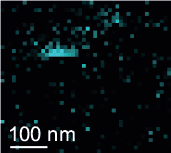
\includegraphics[width=0.3\textwidth]{img/chapitre1/figure12/sequentialScan.png}}\hspace{1em}
        \subfigure[\label{fig-echantillon-deteriore-b}]{%
            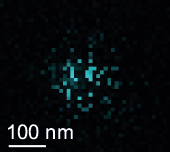
\includegraphics[width=0.3\textwidth]{img/chapitre1/figure12/randomScan.png}}
        \caption{\protect\subref{fig-echantillon-deteriore-a} Exemple d'échantillon détérioré par un faisceau trop énergétique. L'acquisition est réalisée ligne par ligne en commençant au pixel supérieur gauche. \`A un certain stade de l'acquisition, une structure apparaît puis disparaît soudainement. En effet, la structure a été détruite suite à une trop grande accumulation d'énergie, l'acquisition conventionnelle illuminant les positions successives. \protect\subref{fig-echantillon-deteriore-b} Acquisition d'une structure semblable avec un parcours aléatoire et la même énergie par pixel. La structure est elle-aussi détériorée, mais l'échantillonnage aléatoire permet de visualiser la particule avant sa disparition.
            \protect\label{fig-echantillon-deteriore}}
    \end{figure}

    \paragraph{Acquisition ligne par ligne v.s. aléatoire.} Une première solution pour réduire la détérioration de l'échantillon à énergie fixée consiste à échantillonner de manière aléatoire uniforme. En effet, l'acquisition ligne par ligne est très simple à implémenter, mais cette modalité détériore particulièrement l'échantillon puisqu'elle accumule des doses d'énergie sur des pixels voisins. Pour pallier ce problème, des travaux récents ont mis au point un obturateur coupant le faisceau au cours de l'acquisition standard~\cite{beche2016development}, permettant de limiter l'accumulation de charges au niveau local, au prix d'un sous-échantillonnage spatial. 
    %
    Afin d'échantillonner l'ensemble des pixels tout en protégeant l'échantillon, un module de balayage novateur basé sur FPGA a été mis au point au LPS~\cite{tararan2016random, zobelli2019spatial, tence2019following} dont le fonctionnement est décrit sur la figure~\ref{fig-random-scan}. Une de ses caractéristiques principales est de rendre le chemin d'acquisition hautement paramétrable où l'ensemble des positions spatiales sont stockées dans une table. L'ordre des pixels est mélangé aléatoirement lors d'une phase initiale, puis ce chemin aléatoire est chargé. 
    %
    Pour chaque nouvelle position à visiter, le module pilote des bobines magnétiques afin de positionner le faisceau sur l'échantillon tandis que l'acquisition du signal est désactivée à l'aide d'un obturateur de faisceau électrostatique. Une fois la position désirée atteinte, le faisceau illumine l’échantillon uniquement pendant le temps requis pour l’acquisition du signal, temps durant lequel la caméra est en mode d’exposition. Enfin, le faisceau est coupé et déplacé vers la position suivante.
    \begin{figure*}
        \centering
        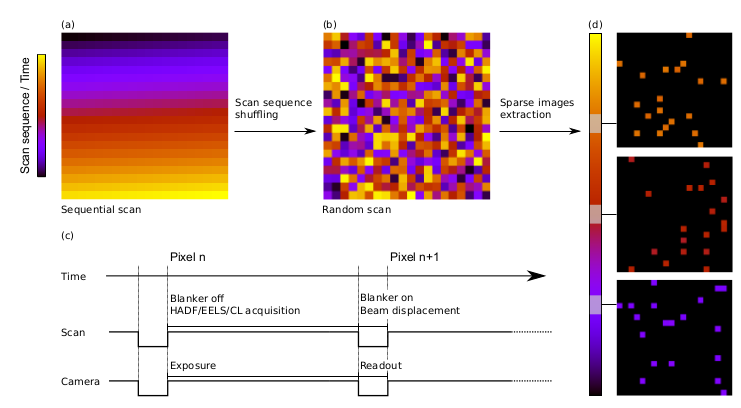
\includegraphics[width=\textwidth]{img/chapitre1/figure18/random-scan-2}
        \caption{\protect\label{fig-random-scan}Principe de l'acquisition ligne par ligne standard (a) et la séquence d'échantillonnage aléatoire (b). L'échelle de couleur représente l'ordre d'acquisition des pixels. (c) Représentation schématique de la synchronisation entre illumination, déplacement du faisceau, obstruction du faisceau, exposition et mesure. (d) Extraction d'images aléatoires partielles à certaines trames temporelles. La figure est issue de~\cite{zobelli2019spatial}.}
    \end{figure*}
    Cette technique d'acquisition permet de répartir la dose d'électron sur l'ensemble de l'échantillon. Cela est mis en évidence à la \cref{fig-echantillon-deteriore-b} puisque la structure spatiale est totalement visible pour une acquisition aléatoire tandis que l'échantillonnage ligne par ligne  détruit prématurément la structure, comme le montre la \cref{fig-echantillon-deteriore-a}. Cette technique permet donc d'augmenter l'énergie délivrée à l'échantillon pour une détérioration égale, et donc d'améliorer la qualité de l'image.
    
    
    \paragraph{Correction de la dérive de l'échantillon.} Comme expliqué à la \cref{sec-prop-eels}, l'échantillon n'est pas nécessairement stable au cours de l'acquisition puisque des gradients de température et des mouvements d'air le font dériver. Dans le cas d'une acquisition ligne par ligne, cela se manifeste par une déformation du réseau atomique, comme le montre la \cref{fig-drift}. Dans le cas d'un échantillonnage aléatoire, cela détériore grandement la résolution spatiale, particulièrement pour les échantillons à échelle atomique. 
    %
    En pratique, la dérive est limitée en laissant l'échantillon se stabiliser après insertion dans le microscope et en s'assurant que l'acquisition soit suffisamment rapide.
    %
    Pour corriger cela, une méthode consiste à extraire $K<P$ sous-acquisitions partielles de l'acquisition aléatoire complète. Chacune de ces acquisitions partielles est alors complétée indépendamment à l'aide d'une méthode de reconstruction (cf \cref{ch-chapter_2}) et le mouvement de l'échantillon est estimé. Les échantillons associés à chaque sous-acquisition sont alors recalés pour compenser la dérive. Cette méthode est appelée \emph{multi-trame} et a été implémentée avec succès en imagerie \gls{haadf} et \gls{eels}~\cite{zobelli2019spatial}. Cette méthode améliore sensiblement la qualité de l'image, mais reste encore très peu utilisée car lourde d'un point de vue expérimental. Enfin, dans le cas d'un échantillonnage ligne par ligne où l'échantillon dérive uniformément, il est également possible de corriger le défaut par déformation géométrique du réseau.

    \paragraph{Débruitage en post-traitement.} L'approche la plus simple pour limiter la détérioration de l'échantillon consiste à réduire la dose d'électrons et à débruiter les données en post-traitement. 
    %
    Pour cela, la technique la plus couramment utilisée pour de nombreuses données spectroscopiques revient à appliquer l'\gls{acp} aux données pour ne conserver que les composantes les plus puissantes, comme cela a été fait pour réduire le bruit spectral en imagerie à échelle atomique~\cite{bosman2007two,dudeck2012quantitative}, par exemple. Cette technique rapide et simple ne permet toutefois pas d'améliorer la qualité spatiale de l'image. D'autre part, certaines études ont mis en évidence des artefacts introduits par l'\gls{acp}, comme un biais présent dans le spectre reconstruit~\cite{lichtert2013statistical, spiegelberg2017can} ou encore l'ajout de structures initialement absentes \cite{mevenkamp2017mm}.
    %
    C'est pourquoi des techniques de débruitage par patch plus récentes et plus efficaces (\cf{} \cref{sec-art-patch}) ont été appliquées afin d'accroître le \gls{snr} du spectre-image tout en limitant les distorsions. Contrairement à l'ACP, celles-ci permettent de débruiter tant spatialement que spectralement. En particulier, des techniques non-locales comme Non-Local Means~\cite{mevenkamp2017mm, mevenkamp2020multimodal} et des approches par \gls{ad} avec apprentissage~\cite{trampert2018ultramicroscopy} ont été appliquées respectivement à des données \gls{eels} et  \gls{sem}. De même, un algorithme non-local appelé Local Low Rank (LLR)~\cite{spiegelberg2018local} a été proposé et appliqué avec succès à des images 2D \gls{haadf} et à des données 3D réalisées après concaténation de cartes d'abondance obtenues par imagerie \gls{stem}-\gls{eels}.
    %
    Cependant, cette façon de préserver l'échantillon pourrait ne pas suffire si la dose maximale autorisée est trop faible. En effet, l'image serait trop dégradée pour être efficacement débruitée et les structures fines pourraient ne plus être détectées. 
    
    
    \section{Positionnement de la thèse}\label{sec-positionnement-these}

    L'équipe STEM du \gls{lps} a très tôt étudié l'ensemble des stratégies présentée dans la section précédente en vue de prévenir la destruction d'échantillons sensibles. Plus précisément, cela a été motivé par l'implémentation du module de balayage décris précédemment afin de contrôler le chemin d'acquisition. Ce système est actuellement installé sur deux microscopes \gls{stem} :
    \begin{itemize}
        \item un VG-HB501 avec un pouvoir séparateur de l’ordre du nm (\cf{} \cref{fig-LPS-micro-a}),
        \item un Nion UltraSTEM 200 équipé d’un correcteur d’aberrations sphériques qui permet d’atteindre un pouvoir séparateur de l’ordre de 0,1 nm (\cf{} \cref{fig-LPS-micro-b}).
    \end{itemize}
    %
    \begin{figure*}
        \centering  % 0.8, 0.5
        \subfigure[\label{fig-LPS-micro-a}]{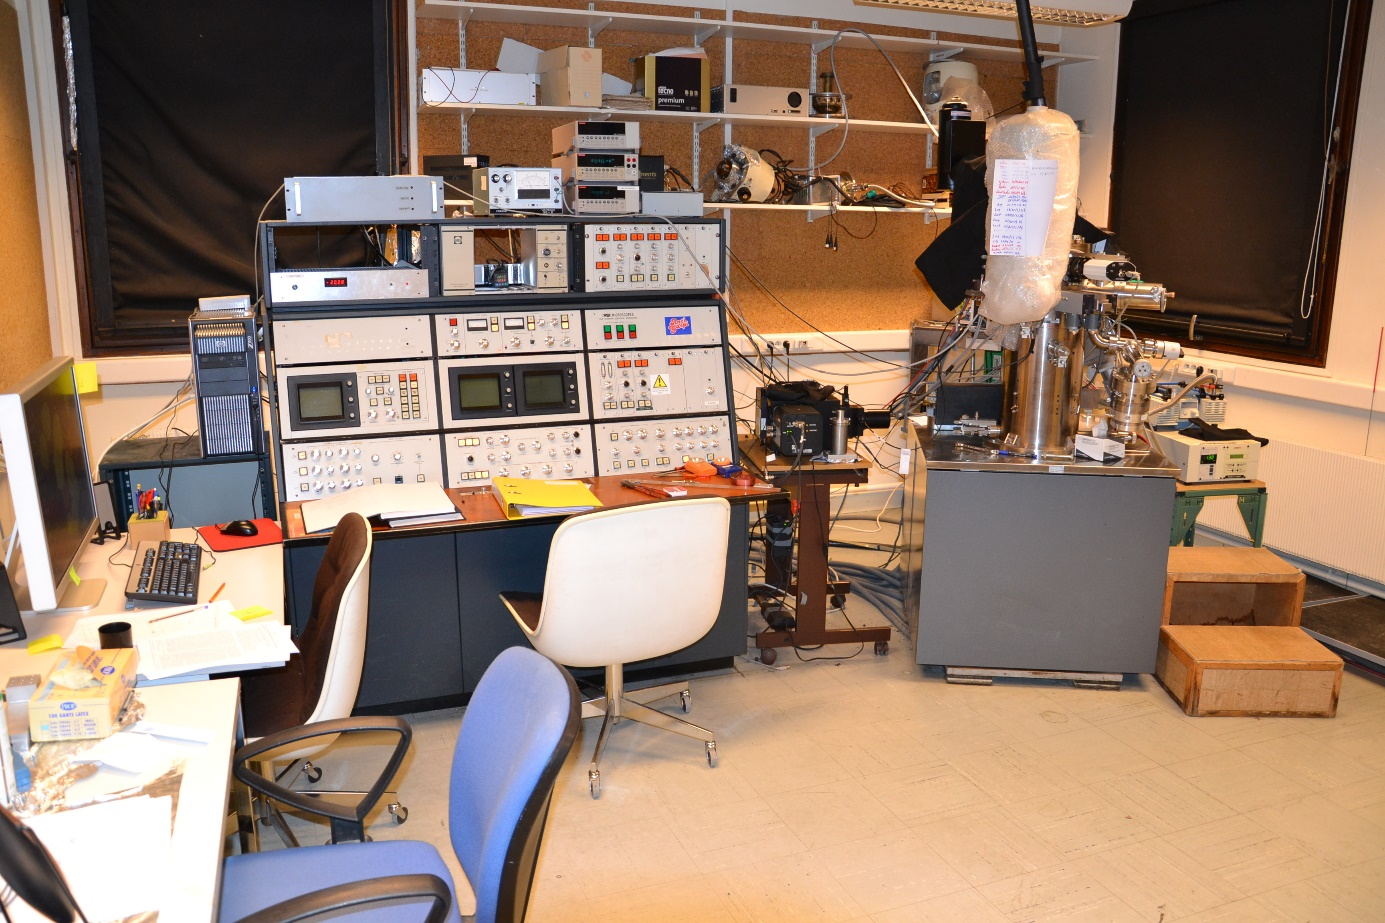
\includegraphics[width=0.5\textwidth]{img/chapitre1/figure13/VG.jpg}}
        \hspace{1em}
        \subfigure[\label{fig-LPS-micro-b}]{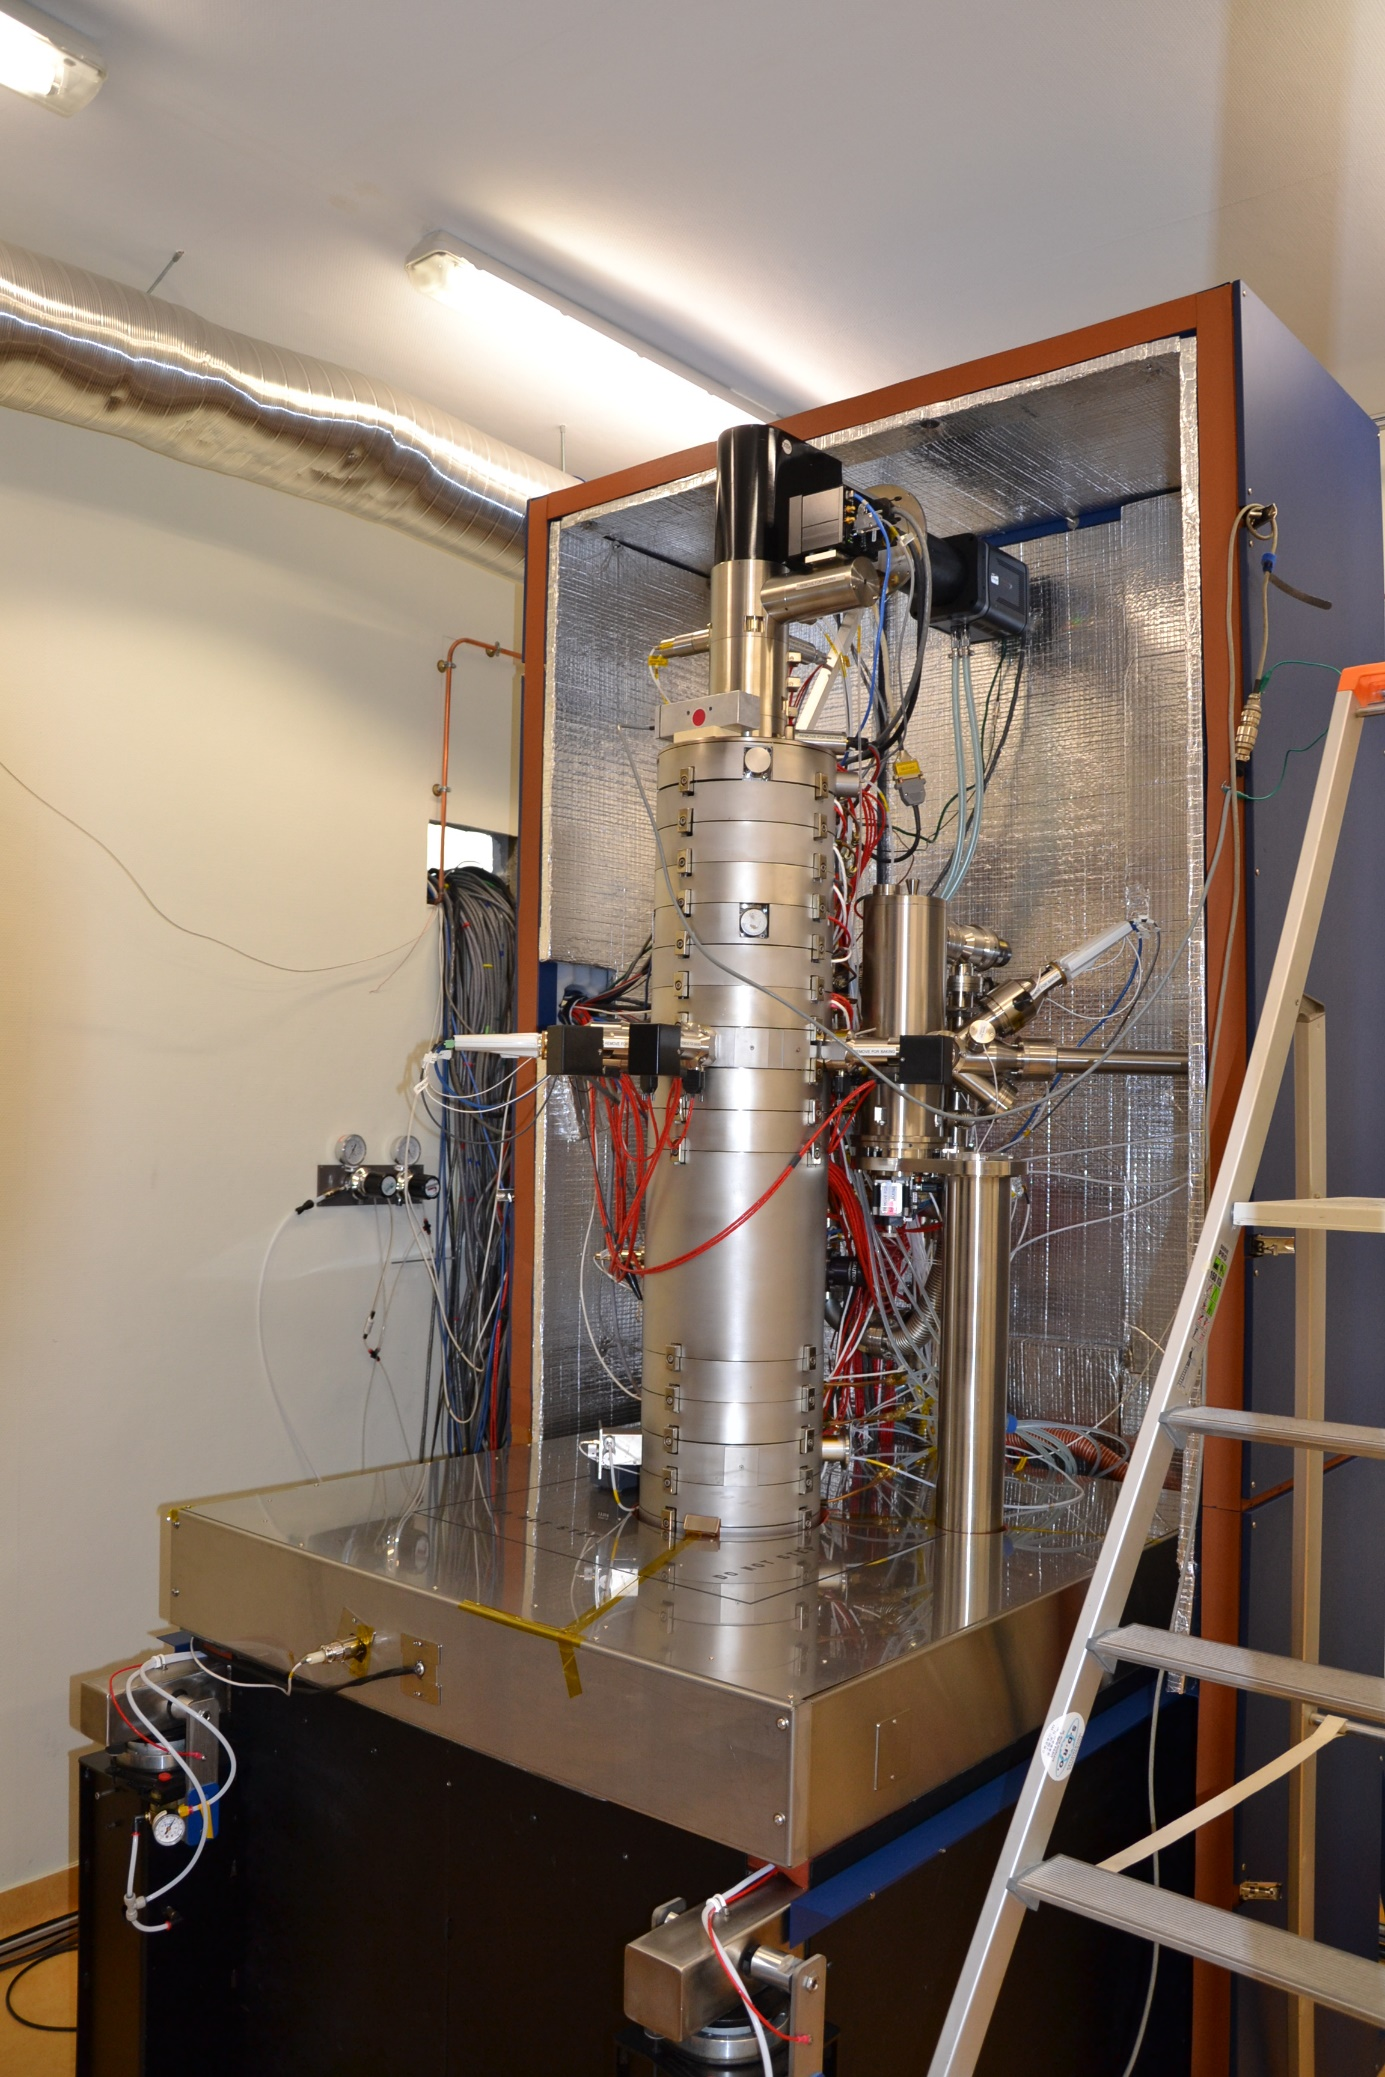
\includegraphics[width=0.4\textwidth]{img/chapitre1/figure13/NION.jpg}}
        \caption{Microscopes en service au \gls{lps} sur lesquels le mode d'acquisition aléatoire est implémenté. \subref{fig-LPS-micro-a} VG-HB501. \subref{fig-LPS-micro-b} Nion UltraSTEM 200.
            \protect\label{fig-LPS-micro}}
    \end{figure*}
    En couplant cette technique d'acquisition à des méthodes de débruitage performantes, on observe une grande amélioration de la qualité de l'acquisition, en particulier pour des temps d'exposition faibles ou des échantillons sensibles. 
    
    Cependant, la grande flexibilité du paramétrage du chemin d'acquisition ouvre la voie à une nouvelle alternative, celle d'accroître la dose d'électron par pixel (et donc le \gls{snr} associé), mais à ne visiter qu'un nombre réduit de positions spatiales en stoppant l'acquisition aléatoire avant son terme. Un algorithme de reconstruction d'image vient enfin compléter les positions manquantes en post-traitement. En paramétrant correctement la dose d'électrons par pixels et le nombre de positions visités, la dose d'électron utilisée est la même que pour les techniques d'acquisition standards et la dégradation de l'échantillon reste identique. 
    %
    Cette façon de procéder a motivé l'usage de techniques de reconstruction performantes issues de la communauté du traitement du signal et il s'agit d'un domaine de recherche très actif en microscopie \gls{stem}~\cite{beche2016compressed,stevens2014potential} et \gls{sem}~\cite{anderson2013sparse} entre autres.
    %
    D'autre part, les performances de cette approche sont intimement liées au choix du chemin d'acquisition et différents travaux présentés à la \cref{sec-art-micro} se sont intéressés à la part d'aléatoire et de régularité à introduire dans ce choix. Certains d'entre eux ont également proposé d'acquérir l'image partielle de manière dynamique en déterminant à chaque instant d'acquisition le pixel à visiter à l'instant suivant.
    %
    Les deux protocoles d'acquisition (débruitage et reconstruction) ont à la fois des avantages et des inconvénients. D'une manière générale, une acquisition à faible dose fournit des informations spatiales plus riches tandis que les données partiellement acquises ont un contenu spectral plus riche. Déterminer quelle approche est la meilleure n'est pas trivial et des études récentes ont comparées ces deux approches~\cite{trampert2018ultramicroscopy} en se basant sur des expériences réalisées sur des images synthétiques et réelles.
    
    Enfin, les techniques de reconstruction sont encore assez marginales dans l'équipe et n'ont été utilisées qu'en cathodoluminescence~\cite{zobelli2019spatial}. 
    %
    Les efforts récents se sont concentrés sur la reconstruction en ligne du spectre-image dans une bande et sa visualisation afin de déterminer si l'élément d'intérêt est présent dans la région observée%
    %
    \footnote[][-2\baselineskip]{%
    Il ne s'agit pas ici de reconstruire le spectre-image complet, mais seulement de sommer des bandes du spectre-image incomplet autours d'un seuil d'intérêt, puis de reconstruire l'image 2D partielle obtenue. Il ne s'agit pas d'une technique d'analyse complètement fiable puisque l'on visualise aussi les effets des seuils précédents, mais cela permet de donner une première idée quant à la présence de l'élément cherché au cours de l'acquisition.}%
    . 
    Cela permettrait d'arrêter prématurément l'acquisition si l'élément est absent, préservant ainsi l'échantillon et accélérant la recherche d'une zone d'intérêt. 
    %
    Une fois ceci fait, des techniques de reconstruction hors-ligne efficaces (et possiblement gourmandes en ressources) seraient nécessaires afin de reconstruire les spectre-images avec une grande précision. Enfin, l'échantillonnage partiel pourrait être utilisé sur les zones étudiées afin de préserver l'échantillon tout en maximisant le \gls{snr}, l'image complète étant restituée a posteriori.
    
    Le travail de thèse présenté dans ce manuscrit a pour but d'évaluer l'apport de l'échantillonnage partiel dans l'acquisition d'échantillons sensibles en imagerie STEM-EELS. Plus précisément, je m'intéresse tout particulièrement à proposer des techniques de reconstruction rapides et efficaces à mettre en \oe{}uvre au cours de l'acquisition. Celles-ci seront comparées à des méthodes de reconstruction plus longues constituant l'état de l'art. Dans ce but, le chapitre~\ref{ch-chapter_2} fera le point sur les méthodes de reconstruction d'images et sur leur utilisation dans la communauté en microscopie.
    
    
    
    
    
    



% ---
\chapter{Etat de l'art}
\dochaptoc
\label{ch-chapter_2}

%
\section{La reconstruction : un problème d'inpainting}

\subsection{Contexte}


De nombreux problèmes en traitement de l'image consistent à corriger une région détériorée ou manquante et, suivant les situations, le masque spécifiant les zones manquantes est plus ou moins structuré. En retouche photographique, par exemple, le masque indiquant les régions à enlever d'une prise de vue~\cite{criminisi2004region} est fortement structuré et les structures sont fines (comme la grille visible à la figure~\ref{fig-inpainting-b}) ou grosses (personnages). Au contraire, le masque peut être très faiblement structuré et réparti, comme à la figure~\ref{fig-inpainting-e} où l'image est aléatoirement et partiellement acquise. Outre les situations où l'acquisition est volontairement lacunaire, les données peuvent souffrir de dysfonctionnements du capteur~\cite{zhang2013hyperspectral} et des bandes (resp. des pixels) peuvent être détériorés, conduisant à un masque fortement structuré et fin (resp. faiblement structuré et réparti).

Pour corriger ces défauts, de nombreuses méthodes proposées ces dernières décennies complètent les régions masquées en se basant sur l'information disponible et non-corrompue. Ainsi, les travaux de Bertalmio \etal{}~\cite{bertalmio2000image} se sont inspirés des techniques de restaurateurs en peinture employés par les musées et ont introduit le terme d'\emph{inpainting} pour désigner ces méthodes de complétion. Des exemples d'inpainting sont affichés aux \crefrange{fig-inpainting-a}{fig-inpainting-c} (resp. \crefrange{fig-inpainting-d}{fig-inpainting-f}) pour un masque structuré fin (resp. pour un masque réparti aléatoire). 

\begin{figure}[b]
    \centering
    \subfigure[\label{fig-inpainting-a}]{
        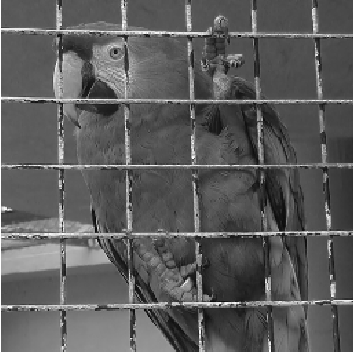
\includegraphics[width=0.25\textwidth]{img/chapitre2/figure1/initial-2.png}}\hspace{1em}
    \subfigure[\label{fig-inpainting-b}]{
        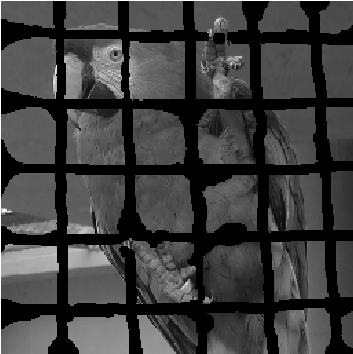
\includegraphics[width=0.25\textwidth]{img/chapitre2/figure1/mask-2.png}}\hspace{1em}
    \subfigure[\label{fig-inpainting-c}]{
        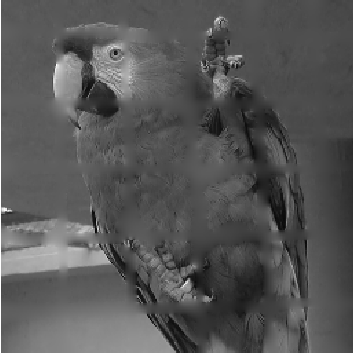
\includegraphics[width=0.25\textwidth]{img/chapitre2/figure1/final-2.png}}\\
    %
    \subfigure[\label{fig-inpainting-d}]{
        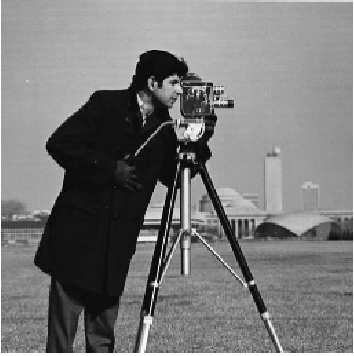
\includegraphics[width=0.25\textwidth]{img/chapitre2/figure2/initial.png}}\hspace{1em}
    \subfigure[\label{fig-inpainting-e}]{
        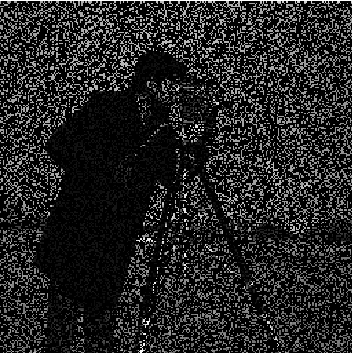
\includegraphics[width=0.25\textwidth]{img/chapitre2/figure2/mask.png}}\hspace{1em}
    \subfigure[\label{fig-inpainting-f}]{
        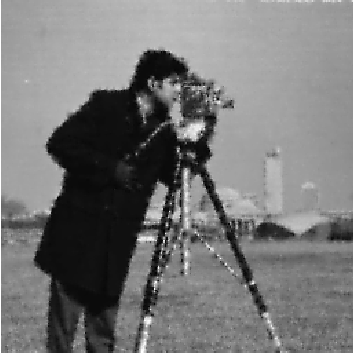
\includegraphics[width=0.25\textwidth]{img/chapitre2/figure2/final.png}}
    \caption{Exemple d'inpainting extrait de~\protect\cite{peyre2011numerical}. \protect\subref{fig-inpainting-a} Exemple d'image destinée à la retouche photographique. \protect\subref{fig-inpainting-b} Les pixels composant la grille sont masqués. \protect\subref{fig-inpainting-c} Résultat après inpainting. \protect\subref{fig-inpainting-d} Exemple d'acquisition complète. \protect\subref{fig-inpainting-e} La même image acquise partiellement. \protect\subref{fig-inpainting-f} Résultat après inpainting.
        \protect\label{fig-inpainting}} 
\end{figure}


La complétion peut être considérée comme un problème inverse dont le modèle d'acquisition est donné à la section suivante~\ref{subsec-direct-inverse-problem}. Plus largement, elle s'inscrit dans le cadre général de l'acquisition comprimée qui fournit des méthodes de restauration avec des garanties théoriques pour les problèmes inverses linéaires sous-déterminés. Les travaux d'Emmanuel Candès, Justin Romberg, Terence Tao et David Donoho~\cite{candes2006near, candes2006stable, donoho2006compressed} ont révolutionné le domaine du traitement du signal. Ceux-ci ont par exemple démontré qu'une image acquise avec une fréquence d'échantillonnage inférieure à celle de Nyquist pouvait être restaurée de manière exacte sous certaines conditions (dont une spécifiant que les données doivent être parcimonieuses dans une certaine base). Cette technique a été appliquée avec succès dans de nombreux domaines incluant l'\gls{irm}~\cite{boyer_algorithm_2014}, l'imagerie ultrasonique~\cite{quinsac_bayesian_2011}, l'astronomie~\cite{bobin_compressed_2008} ou la tomographie en microscopie~\cite{binev2012compressed, jacob2019MM, jacob2018MM}. %
%
Ces résultats ont rendu populaire les problèmes d'inpainting et il s'agit d'un domaine de recherche très actif en microscopie \gls{stem}~\cite{beche2016compressed,stevens2014potential} et \gls{sem}~\cite{anderson2013sparse} entre autres.


La technique d'inpainting est généralement associée à la reconstruction d'images 2D, mais elle s'étend au-delà pour les images multi-dimensionnelles dont une partie des voxels (l'équivalent des pixels pour une image multi-dimensionnelle) sont manquants.
%
La stratégie d'acquisition partielle décrite à la \cref{sec-ech-sensibles} s'inscrit dans ce contexte. En effet, la sonde ne visite qu'une partie de l'échantillon en suivant un chemin généralement aléatoire. Il en résulte des données spatialement sous-échantillonnées que les techniques d'inpainting peuvent compléter.
%
Notons également que ce schéma d'acquisition spatial ne s'accompagne pas d'un sous-échantillonnage spectral puisque, pour chaque position spatiale, le spectromètre \gls{eels} sépare simultanément toutes les pertes d'énergie conduisant à une acquisition complète du spectre. Il en résulte que le masque pour une telle stratégie est \emph{fortement structuré}.


\subsection{Modélisation du problème d'inpainting}\label{subsec-direct-inverse-problem}

Notons $\gls{Y}\in\mathbb{R}^{\gls{M}\times\gls{P}}$ la matrice qui correspondrait aux données \gls{eels} complètes composées de \gls{P} pixels et de \gls{M} canaux. 
%
Comme expliqué à la \cref{sec-ech-sensibles}, faire l'acquisition complète du spectre-image \gls{Y} n'est pas toujours possible dû à la détérioration introduite par le faisceau d'électron sur l'échantillon et c'est pourquoi un sous-échantillonnage spatial est envisagé, comme expliqué à la section~\ref{sec-positionnement-these}.
%
Ainsi, les spectres complets sont acquis en \gls{N} positions parmi \gls{P}, il en résulte un taux d'échantillonnage $\gls{r}=\gls{N}/\gls{P}$. L'ensemble des indices des \gls{N} positions spatiales visitées ainsi que la matrice d'observation sont respectivement notés \gls{I} et \gls{Yi}, où \gls{Yi} est la matrice de taille \taille{M}{N} rassemblant les $N$ colonnes de \gls{Y} indexées par \gls{I}. %

Nous avons vu à la \cref{sec-prop-eels} que le bruit présent dans les données est le mélange de plusieurs contributions avec chacune leur propriétés statistiques. Il en résulte que quantifier chacune de ces contribution est complexe en pratique et les modèles classiquement retenus dans la littérature sont les bruits poissonnien~\cite{egerton2011electron, mevenkamp2015poisson, stevens2018apl}, gaussien~\cite{stevens2014potential, binev2012compressed} et mixte poisson-gaussien~\cite{sanders2020inpainting}. Dans ce manuscrit, nous choisirons de modéliser la détérioration des données avec un bruit indépendant, additif et gaussien. Deux raisons motivent ce choix. D'abord, les paramètres du bruit sont difficiles à caractériser en pratique, si bien que le bruit gaussien plus simple est préféré. Ensuite, les expériences conduites à l'annexe~\ref{sec-bruit-mixte} avec un modèle de bruit mixte n'ont pas permis de mettre en évidence une perte de performances significative par rapport à un modèle gaussien seul. De plus, si une composante poissonnienne émerge particulièrement, des techniques de stabilisation de variance comme la transformée de Anscombe~\cite{anscombe1948transformation} permettent de \guillemets{convertir} le bruit mixte en un bruit gaussien.

Finalement, la matrice observée \gls{Yi} peut être décrite par le modèle suivant :
\begin{equation}
    \gls{Yi} = \gls{X}_{\gls{I}} + \gls{E}
\end{equation}
où \gls{X} est l'image idéle et \gls{E} est un terme résiduel représentant l'erreur de modèle et le bruit d'acquisition. Les éléments de \gls{E} sont supposés être indépendants et identiquement distribués selon une loi gaussienne centrée d'écart type \gls{sig}.

Le problème de reconstruction consiste à estimer un spectre-image de taille \taille{M}{P} complet (et possiblement débruité) \gls{X} à partir de \gls{Yi}. Cependant, cette tâche est mal posée puisque le nombre de paramètres \gls{P}\gls{M} est supérieur au nombre d'observations \gls{N}\gls{M} et la suite de ce chapitre étudiera les approches possibles pour résoudre ce problème inverse.


%
\section{Les différentes classes d'inpainting}

Cette section présente les méthodes de reconstructions classiquement rencontrées dans la littérature en les classant en cinq sections : les techniques d'interpolation, les techniques de \gls{mc} régularisés, les techniques par diffusion, les techniques par patch et les techniques par réseaux de neurones.


\subsection{Les techniques d'interpolation}\label{sec-interpolation}

\paragraph{Présentation du problème d'interpolation.} Le problème d'inpainting peut être vu comme un problème d'interpolation. L'image est alors définie par une fonction $f:\mathbb{R}^3\rightarrow \mathbb{R}$ associant chaque voxel $p\in\mathbb{R}^3$ à une valeur $f(p)\in\mathbb{R}$, connue en un ensemble de points $(s_k)_{k\in\gls{I}}$. Reconstruire l'image, c'est estimer les valeurs prises par $f$ sur un ensemble de points $(m_k)_{k\in \gls{I}^c }$ définis par le masque qu'il soit structuré ou non. 
%
Ce problème est facile en 1D et reste simple en dimension trois à condition que les points masqués soient répartis suivant une maille générée par trois ensembles de coordonnées $\mathcal{J}_x$, $\mathcal{J}_y$, $\mathcal{J}_{eV}$. L'interpolation est plus difficile dans le cas général, comme dans notre situation où le masque est aléatoirement et uniformément généré. L'espace doit alors être découpé en éléments de base, puis la fonction est interpolée sur ces éléments. Par exemple, en 2D, l'enveloppe convexe du nuage de points échantillonnés peut être découpée en un ensemble de triangles à l'aide de la triangulation de Delaunay présentée à l'annexe~\ref{abstr-voronoi-delaunay}. En particulier, chaque triangle de la triangulation a pour sommets des points du nuage et aucun point échantillonné ne se situe à l'intérieur du cercle circonscrit au triangle. L'avantage principale de cette triangulation sa faible complexité : $\mathcal{O}(|\gls{I}|\log |\gls{I}|)$~\cite{lee1980two}, voire $\mathcal{O}(|\gls{I}|\log \log |\gls{I}|)$~\cite{dwyer1987faster} dans de nombreux cas.

\paragraph{Interpolation par \Glsentrylong{ppv}.} L'interpolation par \gls{ppv} est la technique d'interpolation la plus simple et la moins coûteuse. Elle consiste à associer à chaque point à interpoler la valeur prise par $f$ au point échantillonné $s_{k}$ le plus proche. Cela consiste à associer $f(s_{k})$ à tout point $x$ appartenant à la cellule de Voronoi de $s_{k}$, définie par l'ensemble des points plus proches de $s_k$ que de tout autre point de $(s_{k'})_{k'\neq k}$. Le diagramme de Voronoi constitué de l'ensemble des cellules est décrit à l'annexe~\ref{abstr-voronoi-delaunay} et a la même complexité que la triangulation de Delaunay. Cette méthode, bien que très peu coûteuse, est aussi la moins efficace puisque la fonction interpolée est constante par morceaux, ce qui entraîne une erreur de reconstruction élevée. Cela est particulièrement visible sur l'exemple d'interpolation \gls{ppv} donné aux figures \ref{fig-interpolation-a} et \ref{fig-interpolation-d} puisque les cellules de Voronoi apparaissent clairement sur l'image.

Pour lisser davantage la fonction interpolée, une solution consiste à associer au point à interpoler $x$ une pondération des valeurs prises par les points $(s_k)_k$ voisins, c'est-à-dire
\begin{equation}\label{eq-weighted-interp}
    \hat{f}(x) = \sum_{k\in\gls{I}} w_k(x) f(s_k)
\end{equation}%
\begin{marginfigure}%
    \centering
    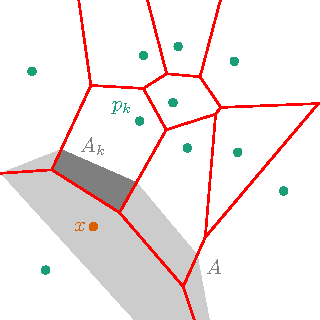
\includegraphics[]{img/chapitre2/figure3/Voronoi_Natural.pdf}
    \caption{Illustration de la méthode par plus proches voisins naturels. Le diagramme de Voronoi associé à l'ensemble de points $(s_k)_k$ connu (en vert) est affiché (en rouge). Lorsque le nouveau point (en orange) est ajouté, une cellule (en gris) est ajoutée au diagramme.}
    \label{fig-natural-weight}
\end{marginfigure}%
\noindent où $w_k(x)$ est le poids de $x$ associé au point échantillonné $s_k$ (la somme des poids vaut 1). Une approche classique consiste à évaluer le diagramme de Voronoi de $(s_k)_{k\in\gls{I}}$ (en rouge à la \cref{fig-natural-weight}), puis une deuxième fois en ajoutant $x$ (la cellule supplémentaire est en gris à la \cref{fig-natural-weight}). Si l'on note $A_k$ l'aire de l'intersection entre cette nouvelle cellule et la cellule précédemment associée à $s_k$ et $A$ l'aire de la nouvelle cellule associée à $x$, alors on pose $w_k(x)=A_k/A$. Cette approche, appelée interpolation par plus proches voisins naturels~\cite{sibson1981interpreting,cazals2006delaunay}, donne de meilleurs résultats que l'interpolation par plus proche voisins, mais elle est aussi plus lourde d'un point de vue calculatoire.

\paragraph{Interpolation pour des ordres supérieurs.} Comme expliqué plus haut, l'interpolation dans le cas multidimensionnel est généralement réalisée en ajustant une fonction d'ordre fixe sur chaque simplexe issu de la triangulation de Delaunay. Ainsi, l'interpolation \gls{ppv} ajuste une fonction constante par morceau sur les sommets du simplexe. Des ordres supérieurs peuvent être utilisés, comme l'interpolation linéaire ou cubique en 1D correspondant respectivement à des fonctions d'ordre 1 et 3. En 2D, cela consiste à ajuster des plans ou des surfaces cubiques par régression aux sommets du triangle. En plus grande dimension, l'interpolation linéaire est réalisée par interpolation barycentrique~\cite{hormann2014barycentric}. Les figures~\ref{fig-interpolation-b}, \ref{fig-interpolation-c}, \ref{fig-interpolation-e} et \ref{fig-interpolation-f} permettent de visualiser le résultat de la régression dans les cas linéaire et cubique.
  
\begin{figure}[h]
    \centering
    \subfigure[\label{fig-interpolation-a}\gls{ppv}]{
        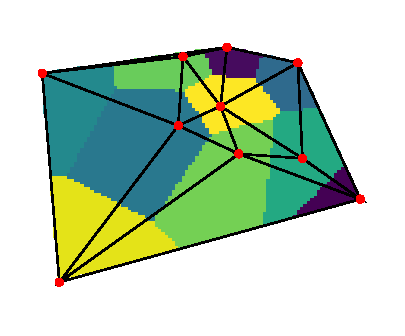
\includegraphics[width=0.29\textwidth]{img/chapitre2/figure4/nearest.pdf}}\hspace{1em}
    \subfigure[\label{fig-interpolation-b}Interpolation linéaire]{
        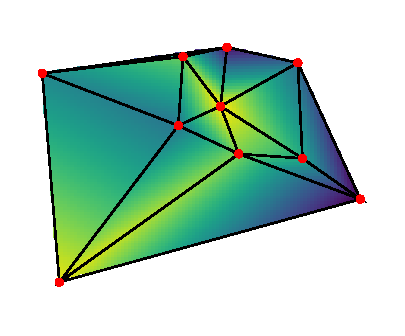
\includegraphics[width=0.29\textwidth]{img/chapitre2/figure4/linear.pdf}}\hspace{1em}
    \subfigure[\label{fig-interpolation-c}Interpolation cubique]{
        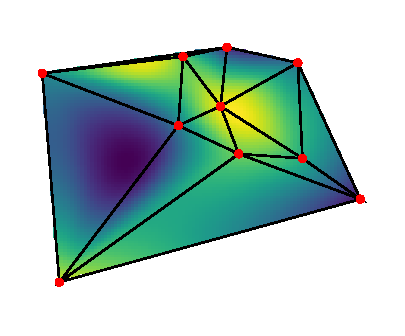
\includegraphics[width=0.29\textwidth]{img/chapitre2/figure4/cubic.pdf}}\\
    \subfigure[\label{fig-interpolation-d}\gls{ppv}]{
        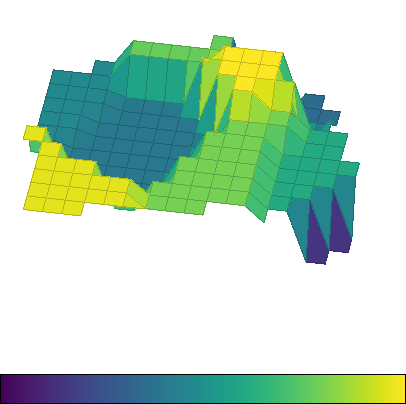
\includegraphics[width=0.29\textwidth]{img/chapitre2/figure4/surf_nearest.pdf}}\hspace{1em}
    \subfigure[\label{fig-interpolation-e}Interpolation linéaire]{
        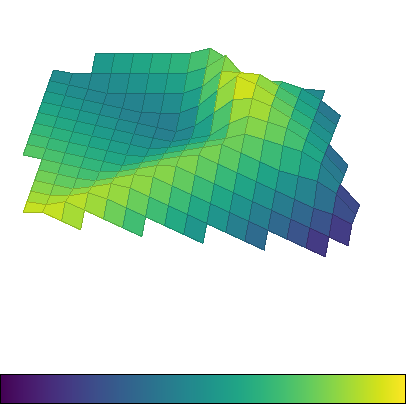
\includegraphics[width=0.29\textwidth]{img/chapitre2/figure4/surf_linear.pdf}}\hspace{1em}
    \subfigure[\label{fig-interpolation-f}Interpolation cubique]{
        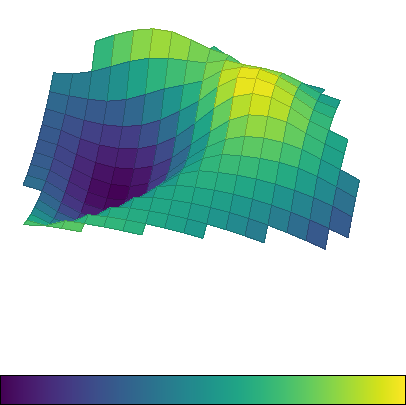
\includegraphics[width=0.29\textwidth]{img/chapitre2/figure4/surf_cubic.pdf}}
    \caption{Exemple d'interpolation sur un nuage de points aléatoirement généré (en rouge). La fonction est interpolée sur l'enveloppe convexe en s'appuyant sur la triangulation de Delaunay représentée en noir. \protect\subref{fig-interpolation-a} Interpolation \gls{ppv}. \protect\subref{fig-interpolation-b} Interpolation linéaire. \protect\subref{fig-interpolation-c} Interpolation cubique. Les fonctions interpolées sont également représentées dans le même ordre sous forme de surfaces aux figures~\subref{fig-interpolation-d} à \subref{fig-interpolation-f} (la résolution spatiale est diminuée pour des raisons d'affichage).
        \protect\label{fig-interpolation}}
\end{figure}


\paragraph{Avantages et inconvénients.} Les méthodes d'interpolation ont pour principal avantage leur faible complexité et leur rapidité, ce qui en font des méthodes populaires en reconstruction en ligne~\cite{sibson1981interpreting, cazals2006delaunay, trampert2018ultramicroscopy}. Néanmoins, elles ne sont pas robustes puisqu'elles s'ajustent aux valeurs disponibles elles-mêmes corrompues. Elles ne permettent pas d'introduire plus d'information a priori que l'ordre de la fonction à interpoler.

\subsection{Les techniques par \glsentrylong{mc} régularisés}\label{sec-MC-regul}

Une approche \emph{variationelle} en inpainting est une méthode calculant l'image reconstruite en minimisant une fonction objectif. En particulier, une technique par \gls{mc} régularisés fournit une image reconstruite \gls{Xh} en résolvant le problème de minimisation suivant~\cite[Section~6.3]{boyd2004convex}
\begin{equation}\label{eq-MC-regul}
    \gls{Xh} = \argmin_{\gls{X}} \frobnorm{\gls{X}_{\gls{I}} - \gls{Yi}} + \lambda \mathcal{R}(\gls{X})
\end{equation}
où $\frobnorm{\gls{X}_{\gls{I}} - \gls{Yi}}$ est le terme d'attache aux données et où l'opérateur $\mathcal{R}$ est une régularisation. Le scalaire $\lambda$ permet d'ajuster l'importance de la régularisation par rapport au terme d'attache aux données. Cette formulation peut s'interpréter comme (si on choisi le paradigme bayésien) l'estimateur du \gls{map} puisque la formule de Bayes donne la fonction de vraisemblance $P(\gls{X}|\gls{Yi}) \propto P(\gls{Yi}|\gls{X}) P(\gls{X})$. En considérant l'opposé de la log-vraissemblance, l'estimée est l'image \gls{X} minimisant la fonction
\begin{equation}
    -\log P(\gls{X}|\gls{Yi}) \propto
    \underbrace{-\log P(\gls{Yi}|\gls{X})}_{\frobnorm{\gls{X}_{\gls{I}} - \gls{Yi}}}
    \underbrace{- \log P(\gls{X})}_{\mathcal{R}(\gls{X})}.
\end{equation}
Il en résulte que le terme d'attache aux données est choisi en fonction du modèle statistique du bruit tandis que la régularisation dépend de l'information a priori disponible pour \gls{X}. Ces méthodes gèrent donc mieux la connaissance du bruit que les techniques d'interpolation et sont ainsi plus robustes. En particulier, le terme d'attache aux données pour un bruit additif gaussien blanc est la fonction coût \gls{mc} $\frobnorm{\gls{X}_{\gls{I}} - \gls{Yi}}$. D'autres fonctions peuvent être utilisés lorsque la statistique du bruit est différente, comme la norme $\ell_1$ pour un bruit laplacien~\cite{frecon2017bayesian} ou la divergence de Kullback–Leibler pour un bruit poissonnien~\cite{ono2013poisson}. Notons encore que les problèmes de \gls{mc} régularisés conviennent que le masque soit structuré ou non et qu'ils sont également utilisés pour la complétion en se basant sur une triangulation, comme c'est le cas en ajustement de surface~\cite{zhong2016surface,cazals2006delaunay}.

Un choix particulièrement classique pour la régularisation est la fonction quadratique $\mathcal{R}(\gls{X}) = \frobnorm{\gls{X}}$, on parle alors de régularisation de Tikhonov. L'avantage de cette forme est que la solution est  donnée par une expression mathématique directe, ne nécessitant qu'une inversion de matrice. La loi a priori de \gls{X} est gaussienne centrée et promeut des données d'amplitude bien répartie autours de la moyenne.

Les techniques de \gls{mc} régularisés sont également d'un intérêt particulier dans le cas de données  parcimonieuses, c'est-à-dire dont la proportion d'entrées non nulles est faible. Dans ce cas, la régularisation idéale est la pseudo-norme $\ell_0$ \footnote{La pseudo-norme $\ell_0$ de \gls{X} vaut le nombre d'entrées non-nulle de \gls{X}. Il ne s'agit pas d'une norme puisque $||\alpha\gls{X}||_0 = ||\gls{X}||_0$ pour tout scalaire $\alpha$ non nul.} puisque celle-ci contraint le nombre d'éléments non-nuls. Malheureusement, résoudre ce problème d'estimation est très compliqué en pratique puisque la norme $\ell_0$ n'est pas convexe et on lui préfère généralement sa relaxation convexe : la norme $\ell_1$ définie par $||\gls{X}||_1 = \sum |\gls{X}_{ij}|$. Cette méthode est souvent appelée Lasso~\cite{tibshirani1996regression} de l'acronyme \emph{least absolute shrinkage and selection operator}. Enfin, il faut noter qu'utiliser la norme $\ell_1$ comme régularisation biaise le résultat. Pour corriger cela, des travaux ont proposé de résoudre le problème inverse en deux temps. D'abord, la technique Lasso est appliquée afin de déterminer les entrées non-nulles de l'estimée. Ensuite, une régression des moindres carrés est réalisée sur ce support. Cette méthode en deux temps est appelée post-LS (pour Least Square) ou encore \emph{refitting}~\cite{belloni2013least, lederer2013trust, deledalle2017clear}.

Utiliser une norme de $\gls{X}$ comme régularisation n'est pas toujours adaptée à l'information a priori disponible,  et l'on préfère généralement pénaliser $\mathcal{A}\gls{X}$ où $\mathcal{A}$ est un opérateur linéaire adapté. Ainsi, une alternative très populaire en traitement du signal consiste plutôt à contraindre le gradient de l'image $\nabla\gls{X}$, conduisant à une régularisation $\mathcal{R}(\gls{X})=\frobnorm{\nabla\gls{X}}$, on parle aussi d'énergie de Sobolev. Cela produit une image lissée. De même, la régularisation $\ell_1$ peut être couplée avec un opérateur linéaire $\mathcal{A}$ pour favoriser la parcimonie du signal dans un cas particulier, par exemple :
\begin{itemize}
    \item si $\mathcal{A}$ est un changement de base telle que $\mathcal{A}\gls{X}$ soit parcimonieuse, la régularisation $||\mathcal{A}\gls{X}||_1$ est adaptée,
    \item si $\mathcal{A}$ est l'opérateur de gradient spatial discret $\nabla$, la régularisation $||\nabla \gls{X}||_1$ appelée \gls{tv} promeut une image ayant peu de contours (l'image résultante est constante par morceaux).
\end{itemize}


\subsection{Les techniques par diffusion}

La diffusion est un processus physique intuitif tendant à équilibrer les différences de concentration au sein d'un fluide sans créer ou détruire de masse. Ce phénomène est régi par l'équation de diffusion suivante
\begin{equation}
    \frac{\partial u}{\partial t} \triangleq \dot{u}(x, y, t) = \mathrm{div} (D(x, y)\cdot \nabla u)
\end{equation}
où $u$ est la concentration, $D$ est le coefficient de diffusion et $\nabla$ est l'opérateur gradient. En traitement de l'image, on identifie la concentration avec la valeur en niveau de gris prise en une position particulière. Si le coefficient de diffusion est constant sur toute l'image, on parle de diffusion \emph{isotrope}, sinon, on parle de diffusion \emph{anisotrope}.

La technique de diffusion la plus simple est la diffusion isotrope en débruitage, conduisant au problème aux dérivées partielles suivant\footnote{Cette équation correspond aussi à l'équation de la chaleur dans le cas où il n'y a pas de source de chaleur.}
\begin{align}
&\dot{u} = D \cdot \Delta u\\
&u(\cdot, t=0) = y
\end{align}
où $\Delta$ est l'opérateur de laplacien spatial discret et $y$ est l'image bruitée. Ce problème est équivalent à un filtrage avec un noyau gaussien d'écart-type $\sqrt{2t}$\footnote{L'image resultante en diffusion n'est pas l'image $u(\cdot, t=\infty)$ puisque celle-ci est constante (la diffusion tend à égaliser les niveaux de gris). Il faut choisir un instant $t^*$ où arrêter la trajectoire et l'image resultante est $u(\cdot, t^*)$.} \cite{weickert1998anisotropic}. Le problème de cette technique est que la diffusion introduit un flou sur les contours de l'image. C'est pourquoi Perona et Malik~\cite{perona1990scale} ont proposé la diffusion anisotropique pour préserver les contours de l'image. Le coefficient de diffusion est diminué au niveau des contours tandis qu'il reste élevé au sein de zones homogènes. Le problème résultant s'écrit
\begin{align}
    &\dot{u}(x, y, t) = \mathrm{div} (D(|\nabla u|^2)\cdot \nabla u)\\
    & D(s) = \frac{1}{1+s^2/\lambda^2} \quad \text{pour $\lambda > 0$}
\end{align}

La technique de diffusion ne suffit cependant pas pour l'inpainting puisque la structure n'est pas propagée et un transport de matière doit être ajouté. Les travaux de Bertalmio \textit{et al.}~\cite{bertalmio2000image} ont été pionniers dans ce domaine et ont été à l'origine du terme \emph{inpainting}. S'inspirant des techniques de restauration en art, ils ont envisagé une technique par transport de matière propageant l'information le long de lignes de niveau (les lignes reliant les points de l'image ayant le même niveau de gris) dans le cas où le masque est structurée. Un terme de diffusion anisotrope était ajouté afin d'éviter que les lignes de niveau ne se croisent. D'autres techniques basées sur la variation totale on suivi~\cite{shen2002mathematical, chan2001nontexture} mais le principe fondamental consiste à propager la structure.

Ces techniques sont très bien adaptées aux images pour lesquelles le masque est très structurée, mais elles ne conviennent pas lorsque l'information est répartie. En effet, ces techniques reposent sur la propagation de contour. Dans le cas où les données sont réparties, aucun contour ne peut être propagé. C'est pourquoi nous n'utiliserons pas ces méthodes dans ce manuscrit.


\subsection{Les techniques par patch}\label{sec-art-patch}

Une extension des méthodes variationelles exploite la redondance spatiale dans l'image (la figure~\ref{fig-redondance-spatiale-search} illustre cette propriété), on parle alors de \emph{méthode par patch} ou \emph{examplar-based}. Elles constituent un ensemble de méthodes très populaires et performantes dont l'intérêt n'a cessé de grandir ces dernières décennies afin de résoudre des problèmes inverses comme le débruitage, l'inpainting ou la déconvolution.

\begin{figure}
    \centering
    \subfigure[\label{fig-redondance-spatiale-search}]{
        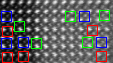
\includegraphics[width=0.7\textwidth]{img/chapitre2/figure5/search.png}}\\
    \subfigure[Atome rouge\label{fig-redondance-spatiale-dic1}]{
        \includegraphics[width=0.25\textwidth]{img/chapitre2/figure5/dico_red.png}}\hfill
    \subfigure[Atome vert\label{fig-redondance-spatiale-dic2}]{
        \includegraphics[width=0.25\textwidth]{img/chapitre2/figure5/dico_green.png}}\hfill
    \subfigure[Atome bleu\label{fig-redondance-spatiale-dic3}]{
        \includegraphics[width=0.25\textwidth]{img/chapitre2/figure5/dico_blue.png}}
    \caption{Illustration de la redondance spatiale en imagerie haute résolution. Une image \gls{haadf} est affichée à la figure~\subref{fig-redondance-spatiale-search} et trois familles de patch sont représentées en rouge, vert et bleu. Les patchs appartenant à une famille donnée sont tous semblables bien que éloignés dans l'image, confirmant l'hypothèse selon laquelle le contenu spatial de l'image est redondant. Les trois premiers atomes d'un dictionnaire appris à l'aide de la méthode mini-batch~\cite{mairal2009online} sont représentés aux figures~\subref{fig-redondance-spatiale-dic1} à \subref{fig-redondance-spatiale-dic3} et correspondent respectivement aux familles de patchs rouge, verte et bleue.
        \protect\label{fig-redondance-spatiale}}
\end{figure}

Ces méthodes sont à opposer aux techniques dites \emph{locales} où une valeur est corrigée en ne la comparant qu'avec son voisinage, comme lorsqu'une image est convoluée avec un masque gaussien en débruitage. Le premier exemple de méthode \emph{non-locale} a été l'algorithme de débruitage Non-Local Means~\cite{buades2005non} qui recherche des patchs semblables dans l'image afin de moyenner les pixels centraux. Par exemple, si l'on considère une famille de patchs de la figure~\ref{fig-redondance-spatiale-search}, les pixels centraux de chacun de ses membres peuvent être débruités en les substituant par leur moyenne. D'autres techniques plus évoluées en débruitage ont suivi, parmi lesquelles Block Matching and 3D filtering (BM3D)~\cite{dabov2007image} et Non Local Bayes~\cite{lebrun2013nonlocal}. Cependant, reconstruire de manière non-locale ne peux se faire naïvement que si le masque est structurée. Par exemple, l'algorithme \gls{ebi}~\cite{criminisi2004region} reconstruit des images partiellement corrompus en remplaçant de manière itérative les patchs manquants par le patch entier lui ressemblant le plus dans la zone connue. Des résultats ont également exprimé Non-Local Means sous forme variationnelle, permettant ainsi des applications en reconstruction d'images dont l'information est répartie~\cite{peyre2008non, unni2018non, arias2009variational, yang2012nonlocal}.

Pour imposer la redondance spatiale, des algorithmes performants cherchent à représenter les patchs de l'image de manière parcimonieuse à l'aide d'\emph{atomes}\footnote{Ici, on ne parle pas des composants élémentaires de la matière, mais bien des patchs constituant le dictionnaire.} contenus dans un \emph{dictionnaire}, on parle alors de méthode par \gls{ad}. Une formulation générique de cette technique peut s'écrire comme le problème d'optimisation suivant~\cite{mairal2009online}
\begin{equation}
    \begin{aligned}
    (\mathbf{D}^*,\mathbf{A}^*) = &\argmin_{(\mathbf{D}, \mathbf{A})}
    \frac{1}{2} \frobnorm{ \mathbf{R}(\gls{Y}) - \mathbf{D A}} + \lambda  || \mathbf{A} ||_1\\
    &\text{tel que } || \mathbf{D}_k ||_2 = 1 \quad \forall k\\
    \end{aligned}
\end{equation}
où $\mathbf{D}$ et $\mathbf{A}$ sont les matrices contenant respectivement les atomes et la décomposition parcimonieuse associé à chaque patch (on parle aussi de \emph{code}). $\mathbf{R}$, quant à lui, est l'opérateur permettant d'extraire les patchs des données et l'image reconstruite est obtenue par $\mathbf{R}^*(\mathbf{D}^*\mathbf{A}^*)$ où $\mathbf{R}^*$ est un pseudo inverse de $\mathbf{R}$. La contrainte permet de normaliser les atomes tandis que la régularisation $|| \mathbf{A} ||_1$ contraint le code à être parcimonieux. 
%
La \cref{fig-redondance-spatiale} donne un exemple d'application de cette méthode pour une image \gls{haadf} haute-résolution, les trois premiers atomes étant affichés sur les figures~\ref{fig-redondance-spatiale-dic1} à \ref{fig-redondance-spatiale-dic3}.
%

%
Cependant, la difficulté de cette approche est que la fonctionnelle à minimiser est non-convexe, si bien que l'on se contente couramment d'un résultat non-équivalent et sous-optimal en alternant l'estimation du code et l'apprentissage du dictionnaire dont les formulations isolées sont convexes.
%
D'une part, si le dictionnaire $\mathbf{D}$ est fixé, l'estimation du code $\mathbf{A}$ consiste à obtenir une représentation parcimonieuse en résolvant 
\begin{align}
    \mathbf{A}^{opt} = &\argmin_{\mathbf{A}} \frobnorm{ \mathbf{R}(\gls{Y}) - \mathbf{DA}}\\
    &\text{tel que}
    \quad
    ||\mathbf{A}_i||_0 \leq N_{\mathrm{max}}\quad\forall i
\end{align}
où $N_{\mathrm{max}}$ est le nombre maximal d'atomes autorisés pour décrire un patch. Orthogonal Matching Pursuit (OMP)~\cite{mallat1993matching, pati1993orthogonal} est un algorithme glouton qui tente d'approximer la solution de ce problème NP-difficile. Son principe consiste à sélectionner le meilleur atome du dictionnaire à chaque itération, à savoir celui qui maximise son produit scalaire avec le résidu, puis à mettre à jour le résidu en appliquant une projection orthogonale du signal que l'on souhaite approximer sur l'espace vectoriel engendré par les atomes précédemment sélectionnés. Cette orthogonalisation est importante puisqu'elle stabilise et accélère la convergence de cet algorithme glouton.
%
D'autre part, une fois l'étape de recherche du code réalisée, le dictionnaire $\mathbf{D}$ doit être mis à jour en conservant $\mathbf{A}$ fixe, non pas en une étape, mais en améliorant chaque atome successivement afin d'alléger le coût. Plus précisément, l'atome $\mathbf{D}_k$ est mis à jour en déterminant le résidu $\mathbf{E}_k$ obtenu en soustrayant la contribution de tous les autres atomes $(\mathbf{D}_{k'})_{k'\neq k}$  des données $\mathbf{R}(\gls{Y})$ et en ne conservant que les patchs utilisant l'atome $\mathbf{D}_k$ dans leur code. La mise à jour de l'atome est enfin réalisée en déterminant le vecteur $\hat{\mathbf{d}}$ résolvant
\begin{equation}\label{eq-dico-ksvd}
    (\hat{\mathbf{a}}, \hat{\mathbf{d}}) = \argmin_{\mathbf{a}, \twonorm{\mathbf{d}}=1} \frobnorm{\mathbf{E}_k-\mathbf{da}}.
\end{equation}
Le code précédemment fixé est mis à jour à l'aide des coefficients corrigé $\hat{\mathbf{a}}$ avant de poursuivre l'amélioration du dictionnaire. L'approximation de rang un donnée à l'équation~\eqref{eq-dico-ksvd} est réalisée en appliquant une SVD tronquée à $\mathbf{E}_k$. La répétition des deux étapes, apprentissage du code par OMP et amélioration du code par SVD, constitue la méthode K-SVD utilisée en débruitage d'images~\cite{elad2006image}.

Toutefois, cette approche contraint le bruit à être uniforme, puisque l'algorithme OMP fait l'hypothèse intrinsèque que le bruit a une structure de sphère dans l'espace des patchs. Pour corriger cela, Mairal \etal{}~\cite{mairal2008tip} ont proposés la construction d'un vecteur $\beta$ de même taille que l'image constitué de poids pour chaque voxel
\begin{equation}
    \beta_p = \frac{\min_{p'\in\text{image}}\sigma_{p'}}{\sigma_p}
\end{equation}
où $\sigma_p>0$ désigne l'écart-type du bruit associé au voxel $p$. L'algorithme OMP est ensuite corrigé en définissant un nouveau produit scalaire dans l'espace des patchs. Plus précisément, chaque élément de cet espace est pondéré par les poids associés au patch courant avant d'appliquer le produit scalaire euclidien. De même, le terme $\mathbf{E}_k-\mathbf{da}$ de l'approximation de rang un à l'équation~\eqref{eq-dico-ksvd} est pondéré à l'aide de ces poids, conduisant à une approximation de rang un pondérée plus complexe. 
%
Cette correction peut être étendue au problème d'inpainting avec un masque faiblement structuré en supposant un bruit de puissance infinie (\ie{} $\sigma_p=\infty$) pour les pixels manquants et en fixant un niveau de bruit constant ailleurs. Ainsi, les pixels manquants se voient affectés d'un poids $\beta_p$ nul, conduisant à des versions masquées de OMP et de l'approximation de rang un. Cette technique pondérée est appelée \gls{wksvd}.

Le problème principal de wKSVD est sa complexité algorithmique, principalement due à la SVD requise par l'étape de mise à jour du dictionnaire. C'est pourquoi l'algorithme \gls{itkrmm}~\cite{naumova2018fast, naumova2017dictionary} a pris le contre-pied en proposant une approche plus rapide ne nécessitant pas de SVD. Elle repose sur l'hypothèse que les données corrompues sont parcimonieuses non pas dans le dictionnaire $\mathbf{D}$ mais plutôt dans une version corrompue du dictionnaire dont le masque dépend du patch considéré et résout le problème comme wKSVD en alternant choix du code et mise à jour du dictionnaire.
%
L'estimation du code est réalisée par seuillage, en ne conservant pour chaque patch que les $N_\mathrm{max}$ atomes corrompus dont le produit scalaire avec les données masquées est maximal. 
La mise à jour du dictionnaire est ensuite réalisée en calculant pour chaque atome la moyenne des résidus sur l'ensemble des patchs corrompus, puis en les normalisant. 
%
Ces travaux soulignent également le besoin de soustraire une composante faible-rang des données afin d'éviter que le dictionnaire soit mal conditionné et que la plupart des atomes soient distordus en direction de la composante faible-rang. C'est pourquoi cette composante est intégrée dans le calcul des résidus, mais sa contribution est soustraite des atomes avant la normalisation lors de la mise à jour du dictionnaire, afin que le dictionnaire soit orthogonal à l'élément faible-rang.

Finalement, d'autre travaux préfèrent avoir recours à des modèles bayésiens afin de déterminer $\mathbf{D}$ et $\mathbf{A}$ à partir des données corrompues. Un algorithme très populaire en microscopie est \gls{bpfa}~\cite{xing2012siam} qui a été conçu initialement pour l'imagerie hyperspectrale. Une description succincte du modèle est donnée ci-dessous tandis que le détail complet est disponible dans~\cite{xing2012siam}. Les atomes $\mathbf{D}_k\in\mathbb{R}^n$ et le bruit $\mathbf{B}$ sont supposés suivre des lois gaussiennes indépendantes tandis que les lignes $\mathbf{A}_{i, :}$ de $\mathbf{A}$ suivent une construction beta-bernouilli. Le modèle hiérarchique complet de BPFA est
\begin{equation}\label{eq-BPFA-model}
\begin{aligned}
    &\mathcal{R}(\gls{Y}) = \mathbf{D A + B} 
    &&\mathbf{E}_i\sim\mathcal{N}(0, \gamma_\mathbf{E}^{-1}\mathcal{I}_n)\\
    %
    &\mathbf{D} = [\mathbf{D}_1, \dots, \mathbf{D}_K]
    &&\mathbf{D}_k\sim\mathcal{N}(0, n^{-1}\mathcal{I}_n)\\
    %
    &\mathbf{A}_{i, :} = \mathbf{Z}_{i, :}\cdot \mathbf{W}_{i, :}
    &&\mathbf{W}_{i, :}\sim\mathcal{N}(0, \gamma_\mathbf{W}^{-1}\mathcal{I}_K)\\
    %
    &\mathbf{Z}_{i, :}\sim \prod_{k=1}^{K}\mathrm{Bernouilli}(\pi_k)
    &&\pi_k\sim\mathrm{beta}\left( \frac{a}{K}, b\frac{K-1}{K} \right)
\end{aligned}
\end{equation}
où $\gamma_\mathbf{E}$ et $\gamma_\mathbf{W}$ sont tirés d'une loi gamma, $a$ et $b$ sont choisis par l'utilisateur et où l'opérateur $\cdot$ désigne le produit terme à terme. L'inférence du modèle~\eqref{eq-BPFA-model} peut être faite en utilisant un échantillonneur de Gibbs, qui est un algorithme de \gls{mcmc}. Tout atome inutilisé après une itération de Gibbs peut être enlevé du dictionnaire et la méthode est itérée jusqu'à ce que l'image n'évolue plus ou que la qualité soit acceptable. Bien que très performant, l'inconvénient majeur de cette technique est sa complexité algorithmique puisque cette méthode est beaucoup plus lente que wKSVD et ITKrMM.

Enfin, il faut bien mettre en avant que la reconstruction d'une image par \gls{ad} ne doit reposer sur les données corrompues \emph{uniquement}. Cette approche ne nécessitant aucune autre donnée est appelée \emph{méthode sans entraînement}. Cependant, il est aisé de reconstruire l'image dès lorsque le dictionnaire est disponible, si bien que les atomes sont parfois appris sur un jeu de données non-corrompues et utilisés ensuite pour la reconstruction, on parle alors de \emph{méthode par entraînement}. Cette approche est connue pour donner de bien meilleurs résultats, mais présente deux inconvénients majeurs :
\begin{itemize}
    \item cela nécessite un grand ensemble d'images propres (appelé données d'entraînement) sur lesquelles apprendre le dictionnaire,
    \item le contenu spatial de l'image à reconstruire doit être similaire au contenu des données d'entraînement.
\end{itemize}
Les performances sont particulièrement dégradées si les structures, leur orientation ou leur échelle diffèrent.


\subsection{Les techniques par réseaux de neurones}\label{sec-methodes-convnets}

Les réseaux de neurones profonds ont connus une popularité grandissante ces dernières décennies pour traiter des données complexes et massives. Leur avantage réside dans leur capacité à extraire les caractéristiques propres à des données pour mieux effectuer leur tâche de classification~\cite{lecun1989backpropagation} ou de détection d'objets~\cite{szegedy2013deep, zhao2019object}, par exemple. Ces techniques sont également d'un grand intérêt pour la résolution de problèmes inverses puisqu'elles permettent d'inverser le processus de dégradation sans nécessiter \emph{aucune information a priori}. En effet, contrairement aux méthodes par \gls{mc} régularisés qui requièrent une régularisation adaptée aux données, les méthodes par réseaux de neurones usent d'un a priori implicite capturé par la paramétrisation du réseau de neurone lors de l'entraînement. Par conséquent, comme pour les méthodes par \gls{ad}, un grand ensemble de données d'entraînement doit être soigneusement choisi. Notons que toutes ces méthodes fonctionnent que le masque soit fortement ou faiblement structuré.

Parmi ces méthodes, les architectures de type auto-encodeur débruiteur~\cite{vincent2010stacked,xie2012image} sont classiquement utilisées en débruitage et en inpainting et la figure~\ref{fig-denoising_deep} en donne une illustration. Elles se caractérisent par une couche de sortie de même taille que la couche d'entrée et comporte plusieurs couches cachées. Elles consistent à fournir en entrée l'image corrompue pour extraire des variables latentes d'intérêt (c'est la partie encodeur), puis à restituer une image corrigée à partir de celles-ci (c'est la partie décodeur). La fonction coût généralement utilisée est la différence quadratique $\frobnorm{\gls{Y}-\gls{X}}$. Ces architectures présentent cependant l'inconvénient d'être denses et l'apprentissage est lourd d'un point de vue calculatoire. C'est pourquoi l'on préfère généralement réduire la dimension en usant de couches convolutives, comme dans~\cite{iizuka2017globally} pour un modèle génératif.
%
\begin{figure}
    \centering
    \includegraphics{img/chapitre2/figure6/denoising_deep.pdf}
    \caption{Illustration d'un auto-encodeur débruiteur. Après entraînement sur des données d'entraînement, l'observation corrompue \gls{Y} est fournie en entrée de l'encodeur afin d'extraire des variables latentes (ou code) caractéristiques de l'image. Un décodeur restitue ensuite une image corrigée \gls{Xh} à partir du code. Le réseau de neurone est dense.
        \protect\label{fig-denoising_deep}}
\end{figure}

Récemment, Ulyanov \etal~\cite{ulyanov2020deep} ont suggéré que les performances excellentes des réseaux de neurones, \ie\ leur capacité à capturer la statistique des images non-corrompues, ne sont pas dues à la phase d'entraînement et au large ensemble d'entraînement associé.
%
Au contraire, la structure du réseau seule serait suffisante à capturer la statistique des données, et cela, sans apprentissage. 
%
Les auteurs ont confirmé cette hypothèse en concevant un réseau génératif, défini par la fonction $f_\theta$ paramétrée par $\theta$, associant à un code $\mathbf{Z}$ une image $\gls{X}=f_\theta(\mathbf{Z})$. Après tirage d'un code aléatoire $\mathbf{Z}$, l'estimation de l'image reconstruite s'écrit donc
\begin{align}
    \hat{\theta} &= \argmin_\theta \frobnorm{\gls{Yi}-f_\theta(\mathbf{Z})_{\gls{I}}}\\
    \gls{Xh} &= f_{\hat{\theta}} (\mathbf{Z}).
\end{align}
En particulier, un réseau convolutif de type auto-encodeur a été utilisé par les auteurs. Cette implémentation affiche des performances supérieures aux autres méthodes par réseaux de neurones et indique que, pour extraire les caractéristiques de l'image à reconstruire, l'image corrompue seule est suffisante. Cette méthode n'a pas été utilisée dans ce manuscrit, faute de temps, mais elle demeure une perspective intéressante.


%We employ DA to perform pre-training in our method because it naturally lends itself to denoising
%and inpainting tasks. DA is a two-layer neural network that tries to reconstruct the original input
%from a noisy version of it. The structure of a DA is shown in Fig.1a. A series of DAs can be stacked
%to form a deep network called Stacked Denoising Auto-encoders (SDA) by using the hidden layer
%activation of the previous layer as input of the next layer.


%
\section{Utilisation des techniques de reconstruction en microscopie}\label{sec-art-micro}

La section précédente a présenté les différentes classes d'algorithmes employées dans la communauté du traitement du signal en vue de reconstruire des images spatialement sous-échantillonnées. Ces techniques ont fortement inspiré les travaux en microscopie visant à limiter la détérioration de l'échantillon en adoptant une approche par acquisition partielle, comme décrit à la \cref{sec-ech-sensibles}.
%
Ainsi, de nombreuses méthodes de reconstruction ont été proposées dans diverses modalités pour compléter l'acquisition partielle et certains travaux les ont comparés pour déterminer lesquelles privilégier.
%
D'autre part, puisque la qualité de reconstruction dépend significativement du chemin d'acquisition, divers travaux ont étudié le masque d'échantillonnage maximisant les performances pour un algorithme de reconstruction donné. Bien que seul le premier aspect ait été étudié dans le présent manuscrit, le second aspect est également d'un intérêt particulier et tous deux seront discutés.
%
La suite de cette section décrira les travaux de la communauté en microscopie traitant de ces aspects en dissociant les approches \emph{sans entraînement} ne nécessitant pas d'autre données que les seules données acquises et les approches \emph{avec entraînement} s'appuyant sur des données d'entraînement.

\subsection{Méthodes sans entraînement}

L'interpolation \gls{ppv} est une solution simple et rapide, autorisant parfois de réaliser conjointement l'acquisition et la reconstruction en temps réel. Cependant, pour éviter que l'image reconstruite soit constante par morceau, on préfère pondérer les valeurs prises par les pixels voisins, comme expliqué à l'\cref{eq-weighted-interp}. La distance entre le pixel à interpoler et le voisin est inversée puis normalisée afin de former la pondération. Cette approche est utilisée en reconstruction d'images \gls{sem} dans~\cite{godaliyadda2018tci}, \gls{edx} dans~\cite{zhang2018reduced, hujsak2018high} et \gls{eels} dans~\cite{hujsak2018high}. L'interpolation par plus proches voisins naturels qui ajuste les poids en se basant sur une représentation de Voronoi est choisie comme alternative pour des images \gls{sem} dans~\cite{trampert2018ultramicroscopy}.

Les méthodes par \gls{mc} régularisés offrent généralement de meilleurs résultats que \gls{ppv} puisqu'elles contraignent l'image reconstruite à suivre un comportement prédéfini, généralement au moyen d'une régularisation adaptée. Un choix classique puisque motivé par le paradigme de l'acquisition comprimée promeut la parcimonie dans une base adaptée, comme la régularisation $\ell_1$ utilisée pour des images de \gls{mfa} dans~\cite{han2018optimal}. Ce type de \gls{mc} régularisés sera noté $\ell_1-\mathrm{\gls{mc}}$ dans la \tabname~\ref{tab-litterature}. %
Dans le cas de structures périodiques (comme c'est le cas pour d'échantillons cristallins), la base de Fourier ou la \gls{dct} peuvent être utilisées. Les auteurs de~\cite{stevens2018apl} ont ainsi proposé une méthode de reconstruction d'image \gls{haadf} reposant sur une transformée de Fourier seuillée, contraignant ainsi la parcimonie dans cette base périodique. La méthode proposée dans~\cite{beche2016development} utilise l'algorithme SPGL1~\cite{berg2008probing} afin de promouvoir la parcimonie dans la base \gls{dct} et reconstruire des images \gls{haadf}. De la même façon, cette régularisation peut être couplée avec une base d'ondelettes pour reconstruire des images \gls{haadf} en ligne~\cite{li2018compressed}. %
%
La régularisation \gls{tv} est aussi classiquement utilisée pour favoriser la reconstruction d'images constantes par morceaux, comme proposé dans~\cite{han2018optimal} pour des données \gls{mfa}. La représentation \gls{dct} par bloc a été couplée avec la \gls{tv} en reconstruction d'images \gls{sem} dans~\cite{anderson2013sparse}.%



Les méthodes par patch offrent généralement de meilleurs performances puisqu'elles exploitent la redondance spatiale et apprennent un espace de représentation adaptée aux données. En particulier, les techniques par \gls{ad} estiment conjointement les atomes constituant un dictionnaire et la représentation parcimonieuse associée. %
%
L'algorithme BPFA est très probablement la méthode par \gls{ad} la plus populaire dans la communauté de microscopie~\cite{xing2012siam}. Elle a été appliquée pour la première fois sur des images \gls{haadf} à échelle atomique~\cite{stevens2014potential} et a été utilisée par la suite dans de nombreux travaux pour le même type de données~\cite{mucke2016practical,kovarik2016implementation}.
%
Les auteurs de BPFA ont également proposé la méthode Kruskal-factor analysis (KFA) comme une extension tensorielle de BPFA~\cite{stevens2017tensor}. KFA a été appliqué à la reconstruction d'images \gls{eels} en se basant sur une acquisition multiplexée d'un spectre-image~\cite{stevens2016mm}.
%
Enfin, l'algorithme expected-patch log-likelihood (EPLL) fait l'hypothèse que la distribution statistique des patchs suit un mélange de lois gaussiennes~\cite{zoran2011from}. Cependant, cet algorithme est particulièrement lent, si bien que les auteurs ont préféré une implémentation simplifiée mais accélérée appelée Fast EPLL (FEPLL) afin de reconstruire des images \gls{sem}~\cite{parameswaran2019accelerating}.
%
En plus des méthodes utilisées dans la communauté de microscopie, wKSVD~\cite{mairal2008tip} et ITKrMM~\cite{naumova2018fast,naumova2017dictionary} apprennent le dictionnaire à partir de données incomplètes sans faire d'hypothèse particulière sur la distribution des patchs. Il s'agit pourtant de méthodes de l'état de l'art et elles seront considérées dans la suite de l'étude.

Afin d'atteindre de meilleures performances avec une dose réduite d'électron, plusieurs chemins d'acquisition ont été proposés, comme l'échantillonnage aléatoire de lignes horizontales~\cite{kovarik2016implementation,han2018optimal}, l'échantillonnage mixe régulier-aléatoire~\cite{stevens2018apl}, les chemins en spirale~\cite{sang2017dynamic,li2018compressive,han2018optimal} ou enfin les chemins en forme de carré~\cite{han2018optimal}.
%
Ces résultats tendent à montrer que les performances optimales sont atteintes par des acquisitions semi-aléatoires, qui introduisent de l'aléatoire dans des structures régulières, ce qui évite les zones masquées de grande dimension. % 
%
Finalement, des améliorations conséquentes en reconstruction ont été rendues possibles par l'acquisition adaptative qui sélectionne le pixel à échantillonner à partir des données précédemment acquises. Dans~\cite{dahmen2016feature}, les auteurs proposent de faire un premier échantillonnage à bas \gls{snr} afin de localiser les contours de l'image. Une seconde acquisition à \gls{snr} élevé est ensuite effectuée sur ces contours seulement. Enfin, les parties lisses de la première image sont filtrées tandis que les contours sont remplis avec les pixels issus de la seconde acquisition. Un schéma d'acquisition adaptative alternatif proposé dans~\cite{dahmen2019adaptive} consiste à localiser de manière itérative des points d'intérêt à échantillonner. Les techniques d'acquisition adaptatives partielles avec entraînement sont présentées à la section suivante.

\subsection{Méthodes avec entraînement}

Contrairement aux méthodes sans apprentissage qui reconstruisent l'image complète à partir des seules données acquises, les méthodes avec entraînement apprennent un opérateur en exploitant des données d'entraînement. Par exemple, l'algorithme \gls{goal} apprend un dictionnaire en maximisant la parcimonie de la représentation des données d'apprentissage~\cite{hawe2013analysis}. Le dictionnaire estimé est ensuite utilisé afin de reconstruire les données de test. De manière similaire, \gls{ebi} qui est initialement une technique sans apprentissage peut être adapté afin de tirer parti de données d'apprentissage. Pour cela, au lieu d'extraire le patch à copier du voisinage, comme c'est le cas dans l'implémentation conventionnelle de \gls{ebi}, ce patch est choisi parmi un dictionnaire appris auparavant sur des images non-corrompues. Cette stratégie est suivie dans~\cite{trampert2018exemplar} pour reconstruire des données 3D en \gls{sem}. \gls{goal} et la version avec apprentissage de \gls{ebi} ont été appliqués dans~\cite{trampert2018ultramicroscopy} pour des images 2D en \gls{sem}, mais BPFA semblait donner de meilleurs résultats.

Les approches avec apprentissage peuvent aussi être envisagées afin de décider quelle position devrait être échantillonnée pour minimiser la distorsion après reconstruction. En effet, la position des pixels échantillonnés impacte grandement la qualité de la reconstruction lorsque les données sont sous-échantillonnées~\cite{trampert2018ultramicroscopy}. Pour améliorer cette qualité, l'algorithme SLADS (supervised learning approach for dynamic sampling) apprend une fonction (appelée réduction de distorsion espérée (RDE)) indiquant quelle position devrait être échantillonnée afin de réduire la distorsion au maximum~\cite{godaliyadda2018tci}. Cette étape d'apprentissage repose sur une liste de caractéristiques et sur des données labellisées et a été utilisée pour dynamiquement échantillonner des images \gls{sem}.
%
Cette méthode a aussi été appliquée à des données \gls{edx} dans~\cite{zhang2018reduced}. Pour cela, un réseau de neurones convolutif classe les spectres des données test et la fonction RDE est calculée simultanément pour toutes les classes. %
%
Le papier~\cite{hujsak2018high} a ensuite modifié cette approche pour permettre des mélanges d'éléments en \gls{eels} et en \gls{edx}. Toutes ces approches requièrent une technique de reconstruction rapide et l'interpolation pondérée \gls{ppv} a été utilisée.



%
\section{Contribution de la thèse}

\begin{mylandscape}
    \begin{normaltable}[]
        \centering
        \bgroup
    \renewcommand{\arraystretch}{1.2}
    \begin{tabular}{>{\arraybackslash\centering}m{3cm}*{5}{c}}
        \toprule
        \multirow{2}*{Famille}& \multirow{2}*{Méthode}& \multicolumn{2}{c}{Travaux}& 
        \multirow{2}*{Temps d'exécution}& \multirow{2}*{Précision}\\
        %
        &&2D&3D&&\\
        %
        \midrule
        %
        \multirow{2}*{Interpolation} & \gls{ppv} & - & - & \plusfa[3] & \minusfa[2]\\
        %
        & Voisinage pondéré & \cite{sibson1981interpreting, cazals2006delaunay, trampert2018ultramicroscopy}&
        - & \plusfa[2] & \minusfa[1]\\
        %
        \midrule
        %
        \multirow{2}*{\gls{mc} régularisés}&
        $\ell_1$-\gls{mc} & \cite{han2018optimal,beche2016development,li2018compressed,anderson2013sparse}& -
        & \plusfa & \plusfa\\
        %
        & TV-\gls{mc} & \cite{han2018optimal} & - & \plusfa[1] & \plusfa\\
        %
        %
        \midrule
        %
        \multirow{6}{3cm}{\centering Méthode par \gls{ad}}&
        BPFA & {\cite{stevens2014potential,trampert2018ultramicroscopy}} &
        \textit{\cite{xing2012siam}} & \minusfa[3] & \plusfa[3]\\
        %
        & EBI & \cite{trampert2018ultramicroscopy} & {\cite{trampert2018exemplar}} &
        \minusfa[1] & \plusfa[2]\\
        %
        & FEPLL & \textit{\cite{parameswaran2019accelerating}},\cite{hujsak2018high} &
        - & \minusfa[1] & \plusfa[2]\\
        %
        & wKSVD & - & \textit{\cite{mairal2008tip}} & \minusfa[2] & \plusfa[2]\\
        %
        &
        ITKrMM & \textit{\cite{naumova2018fast}} & \textit{\cite{naumova2017dictionary}}&
        \minusfa[1] & \plusfa[2]\\
        %
        & GOAL & \textit{\cite{hawe2013analysis}},\cite{trampert2018ultramicroscopy}&
        - & \minusfa[1] & \plusfa[2]\\
        %
        \bottomrule
    \end{tabular}
    \egroup
        \caption{Comparaison des méthodes proposées dans la littérature en microscopie pour le reconstruction d'images partiellement échantillonnées. Des références supplémentaires n'étant pas issues de la littérature en microscopie sont données en italique. Le temps d'exécution et la précision sont évaluées qualitativement en se basant sur les résultats des chapitres suivants.%
            \protect\label{tab-litterature}}
    \end{normaltable}
\end{mylandscape}

Dans cette étude, j'étudie des méthodes de reconstruction rapide pour les données \gls{stem}-\gls{eels} acquises partiellement. En particulier, une motivation consiste à réduire le temps de calcul associé à l'étape d'inpainting en vue de l'insérer dans le processus d'acquisition. L'expérimentateur devrait être capable de visualiser le spectre-image complet au cours de l'acquisition en vue de stopper prématurément l'échantillonnage si la zone ne se révèle pas intéressante, ce qui permettrait de préserver l'échantillon. Cela requiert à la fois un temps de calcul réduit et une bonne précision. En plus de ce processus dynamique, l'expérimentateur devrait être capable de raffiner le spectre-image reconstruit a posteriori. Dans ces conditions, des algorithmes plus performants mais nécessitant plus de temps de calcul pourront être utilisés. 


Afin de déterminer l'approche à privilégier, la \tabname~\ref{tab-litterature} résume l'état de l'art en microscopie réalisé dans la section précédente. Les méthodes y sont notées en fonction de leur complexité et de leurs performances et groupées selon trois grandes familles : l'interpolation, les \gls{mc} regularisés et les méthodes par \gls{ad}. Pour chaque méthode, les travaux issus de la littérature sont fournis et séparés selon que les données reconstruites soient des images 2D mono-bandes (\eg{} \gls{haadf}) ou des spectre-images 3D (\eg{} \gls{eels}).

Parmi les méthodes compatibles avec les données \gls{eels}, \gls{ppv} est rapide mais les performances en reconstruction sont généralement mauvaises tandis que les méthodes par \gls{ad} sont très efficaces mais sont très lourdes en temps de calcul, tout particulièrement lorsque des patchs 3D sont appris. Par conséquent, cet état de l'art met en évidence une lacune : aucune technique n'est disponible pour reconstruire précisément un spectre-image spatialement sous-échantillonné suffisamment rapidement pour l'inclure dans un processus expérimental d'acquisition en ligne. D'autant que l'acquisition et la reconstruction rapide d'un spectre-image \gls{eels} n'a suscité que peu d'intérêt en comparaison de sa contrepartie hyperspectrale en observation de la Terre~\cite{zhang_hyperspectral_2014, chayes_pre_processing_2017, golbabaee_hyperspectral_2012, chen_inpainting_2012}.

Une alternative pour systématiquement reconstruire un spectre-image consiste à traiter les images 2D associées à chaque canal \emph{séparément} et \emph{en parallèle}. Notons d'ailleurs que \gls{ppv} fonctionne de cette façon lorsqu'il reconstruit un spectre-image spatialement sous-échantillonné. Cependant, cette approche est sous-optimale : la tâche de reconstruction est censée être plus efficace en s'appuyant sur les données 3D complètes puisque les bandes du spectre-image sont corrélées. Des stratégies similaires consisteraient à ne reconstruire que les images associées à un ou plusieurs canaux d'intérêt nécessaires pour la cartographie d'éléments. Cependant, cette approche serait aussi sous-optimale quand aucun a priori serait disponible concernant l'échantillon à observer.

Pour conclure, ni l'interpolation \gls{ppv}, ni les méthodes par \gls{ad} ne sont adaptées à la reconstruction précise en ligne et seulement les méthodes par \gls{mc} allient précision et charge calculatoire réduite. C'est donc ce type d'approche qui a été étudié dans la suite de ce manuscrit. Et puisque les performances des méthodes par \gls{mc} régularisés dépendent fortement de l'information disponible a priori, la reconstruction d'images \gls{eels} spatialement lisses sera étudiée dans le \cref{ch-chapter_3} tandis que les échantillons cristallins le seront dans le \cref{ch-chapter_4}. Remarquons finalement que les méthodes par \gls{ad} sont les techniques les plus performantes disponibles et qu'elles conviennent parfaitement à l'étape de raffinement effectuée a posteriori. Le but poursuivi n'est pas de battre ces méthodes en termes de performance, mais de proposer des techniques efficaces ayant une faible charge calculatoire.  Ces méthodes particulièrement performantes ne seront pas étudiées par la suite et ne servirons que de comparaison aux approches proposées. 



%
% Contribs
%

\begin{fullwidth}
	\part{Inpainting rapide en EELS}
\end{fullwidth}

% ---
\chapter{Inpainting rapide d'images spatialement lisses}
\label{ch-chapter_3}
\dochaptoc
%
\section{Contexte des données EELS spatialement lisses}

Ce chapitre se focalise sur les images spatialement lisses, \ie{}, dont l'évolution spatiale est lente. En microscopie STEM-EELS, deux situations peuvent aboutir à ce type d'image : soit l'image est basse résolution, soit l'échantillon est amorphe ou mal orienté.

\subsection{Contexte des images basses résolution}\label{sec-donnees-sous-echantillonnees}


Les images basse résolution déjà présentées à la \cref{sec-prop-eels} sont acquises sur des échelles relativement grandes (typiquement 100nm) afin de visualiser les structures présentes dans l'échantillon. 
%
Or, le nombre de pixels que l'on peut s'autoriser à échantillonner est limité afin d'empêcher une trop grande détérioration de l'échantillon. 
%
C'est pourquoi les images \gls{eels} acquises sur de telles échelles sont volontairement fortement sous-échantillonnées, elles ont généralement une résolution relativement faible comparée au pouvoir séparateur de l'instrument, \ie\ qu'un pixel d'une image basse résolution représente de nombreuses colonnes atomiques. 
%
Par exemple, l'image \gls{haadf} (acquise simultanément à l'image \gls{eels}) donnée sur la figure~\ref{fig-BR-haadf-b} a une taille de pixel de \np[nm]{2}, soit approximativement 20 colonnes atomiques, ou encore 2 fois (resp. 20 fois) le pouvoir de séparation du VG-HB501 (resp. du Nion UltraSTEM 200) dont dispose le \gls{lps}.
%
Il en résulte que, dans le cas d'une acquisition complète du spectre-image, un problème de super-résolution (couplé à du débruitage) peut être posé afin de restituer une image dont la résolution est identique au pouvoir séparateur de l'appareil. \`A cela vient s'ajouter le problème d'inpainting formulé dans la section précédente lorsque l'acquisition est incomplète. Dans le cadre de cette étude, le problème de super-résolution ne sera pas considéré et les résolutions des images acquise et reconstruite seront les mêmes.

En ce qui concerne les images basse résolution, les distorsions associées à l'acquisition, en particulier la dérive de l'échantillon, sont supposées être négligeables par rapport à la taille du pixel (ce qui n'est pas vrai pour les données haute résolution comme nous le verrons au \cref{ch-chapter_4}). Et puisque la résolution de l'image est faible, celle-ci est généralement spatialement lisse et rentre dans le cadre de ce chapitre.

Il faut noter que l'acquisition d'une image \gls{haadf} requiert un temps d'exposition de l'ordre le la microseconde, contre un temps de l'ordre de la milliseconde pour l'acquisition \gls{eels}, ce qui permet de visiter davantage de pixels à dose totale fixée. En général, cela permet de visualiser les structures suivant un angle de vue plus large et de localiser la zone d'intérêt, comme le montre la \cref{fig-BR-haadf-a}. A contrario, l'acquisition \gls{eels} (ainsi que l'image \gls{haadf} acquise de manière simultanée) est très localisée et sa taille est très réduite, comme le montre la \cref{fig-BR-haadf-b}.

\begin{figure}[t]
    \centering
    \subfigure[\label{fig-BR-haadf-a}]%
    {\includegraphics[height=0.5\textwidth]{img/chapitre3/figure1/haadf-LR-2.png}}
    \hspace{1em}
    \subfigure[\label{fig-BR-haadf-b}]%
    {\includegraphics[height=0.35\textwidth]{img/chapitre3/figure1/haadf2.png}}\\
    %
    \caption{\protect\label{fig-BR-haadf}
        Images \gls{haadf} basse résolution d'un échantillon organique. 
        \subref{fig-BR-haadf-a} Acquisition \gls{haadf} avec prise de vue étendue afin de localiser la zone d'intérêt représentée en rouge. L'image est de taille 907$\times$907 pixels. 
        \subref{fig-BR-haadf-b} Acquisition \gls{haadf} prise en même temps que des données \gls{eels}. La résolution spatiale est donc la même. L'image est de taille 51$\times$51. 
    }
\end{figure}


\subsection{Images spatialement lisses en haute résolution}

Dans le chapitre~\ref{ch-chapter_4}, nous discuterons des images haute résolution à échelle atomique, tout particulièrement lorsque l'échantillon est cristallin et l'image est spatialement périodique.
%
Or, certains échantillons sont partiellement amorphes ou mal orientés si bien qu'aucune structure périodique ne peut être obtenue, comme c'est le cas sur la figure~\ref{fig-materiau-amorphe-a} pour des filaments d'ADN marqués à l'uranium et au thorium.
%
Ou encore, la forme du composé ne permet pas d'obtenir une image atomique définie, comme c'est le cas pour les nanotubes de carbone de la figure~\ref{fig-materiau-amorphe-b}.
%
Dans ces situations, l'image haute-résolution peut être suffisamment lisse pour être considérée dans le cadre applicatif de ce chapitre. Toutefois, les expériences menées n'utiliseront pas de telles images, mais des images basse résolution.  

\begin{figure}[h]
    \centering
    \subfigure[\protect\label{fig-materiau-amorphe-a}]{\includegraphics[height=5cm]{img/chapitre3/figure13/example-sc.png}}
    %
    \hspace{1em}
    %
    \subfigure[\protect\label{fig-materiau-amorphe-b}]{\includegraphics[height=5cm]{img/chapitre3/figure13/example3.png}}
    %
    \caption{Exemples d’images HAADF haute résolution ne présentant pas de structure atomique périodique. 
        \protect\subref{fig-materiau-amorphe-a} Atomes de Th et de Tb déposés sur un film de C amorphe très mince ($\approx$~\np[nm]{4} d'épaisseur)~\cite{march2014adressing}.
        \protect\subref{fig-materiau-amorphe-b} Métallo-fullerènes encapsulés dans des nanotubes de carbone~\cite{colliex2012capturing}.
        \protect\label{fig-materiau-amorphe}}
\end{figure}


\subsection{Information a priori et régularisations}\label{subsec-BR-reguls}

Dans le chapitre précédent~\ref{ch-chapter_2}, nous avons montré l'intérêt d'une technique par \gls{mc} régularisés en vue de reconstruire une image \gls{eels} sous-échantillonnée de manière efficace et rapide. Plus précisément, restituer un spectre-image complet \gls{X} à partir de mesures partielles \gls{Yi} est un problème inverse mal posé et la qualité de la méthode par \gls{mc} régularisés repose sur le choix de régularisations appropriées.
%
Les travaux présentés dans ce chapitre exploitent deux types différents d'information intrinsèque partagé par les données \gls{eels} spatialement lisses, à savoir la régularité spatiale et la propriété faible-rang dans le domaine spectral discutées ci-dessous.

\paragraph{Régularisations spatiales.} Dans le cadre applicatif de ce chapitre, les spectre-images \gls{eels} seront supposés spatialement lisses, que ce soit dû, par exemple, à une faible résolution de l'image ou à un échantillon amorphe. Par conséquent, on minimisera l'énergie du gradient de l'image \frobnorm{\nabla \gls{X}}, aussi appelé énergie de Sobolev, ce qui impose la régularité spatiale dans chaque bande.

\paragraph{Régularisations spectrales.} La \cref{sec-acp-redondance} a mis en lumière une propriété particulière des images multibandes telles que les images hyperspectrales issues de la télédétection ou encore les spectre-images \gls{eels} étudiés dans ce manuscrit, à savoir leur grande corrélation spectrale et la propriété faible-rang dans le domaine spectral. Cependant, promouvoir la structure faible-rang du spectre-image \gls{X} nécessite la minimisation du rang de \gls{X}, ce qui est un problème NP-difficile. Une alternative consiste à minimiser la norme nucléaire $||\gls{X}||_*$ définie comme la norme $\ell_1$ des valeurs singulières de \gls{X}. Cette relaxation convexe populaire conduit à un problème convexe facilement optimisable~\cite{recht2010guaranteed}.

Nous considérerons également une régularisation spectrale alternative basée sur une contrainte de sous-espace. En s'inspirant de stratégies déjà suivies dans \cite{wei2015bayesian} et \cite{wei2015fast} pour réaliser la fusion d'images multi-bandes, l'idée principale est d'estimer a priori le sous-espace linéaire où les spectres \gls{eels} évoluent et de reconstruire l'image complète dans ce sous-espace. Plus précisément, le sous-espace d'intérêt est d'abord estimé en appliquant une \gls{acp} aux données observées. Ensuite, le problème d'optimisation~\eqref{eq-MC-regul} est reformulé afin de projeter le spectre-image sur les composantes principales les plus puissantes. Les puissances des composantes principales sont de plus exploitées afin de définir une régularisation spectrale pondérée appropriée.

Les régularisations spatiale et spectrale décrites précédemment conduisent à deux formulations variationnelles différentes pour le problème de reconstruction de spectre-image \gls{eels}, qui sont détaillées dans les sections suivantes.

\newpage
%
\section{La méthode S2N}

\subsection{Formulation}\label{s2n-formulation}

\'Etant donné le modèle direct détaillé à la \cref{subsec-direct-inverse-problem} et les caractéristiques spatiale et spectrale du spectre-image \gls{eels} discutées à la \cref{subsec-BR-reguls}, la première méthode de reconstruction consiste à résoudre le problème d'optimisation suivant
\begin{equation}\label{eq-s2n}
    \gls{Xh} = \argmin_{\gls{X}\in\mathbb{R}^{\taille{M}{P}}} %
    %
    \frac{1}{2} \frobnorm{\gls{Yi} - \gls{X}_{\gls{I}}}  +
    \frac{\gls{ls2n}}{2} \frobnorm{\gls{X}\gls{D}} + 
    \gls{ms2n} ||\gls{X}||_*
\end{equation}
où \gls{D} est l'opérateur de gradient spatial discret appliqué à tous les canaux indépendamment. Ce problème d'optimisation appelé \gls{s2n} repose sur deux paramètres \gls{ls2n} et \gls{ms2n} ajustant respectivement les poids des régularisations spatiale et spectrales. Le choix de ces paramètres est discuté dans la section suivante.


\subsection{Estimation des paramètres de régularisation}\label{sec-s2n-param-tuning}

Nous allons à présent discuter le choix des paramètres \gls{ls2n} et \gls{ms2n} ajustant les régularisations spatiale et spectrale dans la fonction objectif de \gls{s2n} décrite à l'équation~\eqref{eq-s2n}. Afin d'ajuster correctement la paire de paramètres\footnote{Afin d'alléger les notations, les lettres \gls{s2n} en indice sont omises dans cette section.} $(\lambda,\mu)$, et en notant $y_{m,\gls{I}(n)}$ la $m$\textsuperscript{ième} composante du spectre  $\gls{Y}_{\gls{I}(n)}$ mesuré à la position spatiale indexée par $\gls{I}(n)$, la stratégie proposée repose sur l'hypothèse suivante
\begin{equation}
    \mathrm{E}\left[ \left(  y_{m,\gls{I}(n)} - x_{m,\gls{I}(n)}  \right)^2 \right] = \gls{sig}^2
\end{equation}
qui met en relation la variance du bruit $\gls{sig}^2$ avec l'erreur de reconstruction attendue en chaque bande et en chaque pixel.
%
Partant de cette hypothèse, choisir la solution optimale
$\gls{Xh}^{\textrm{opt}} \triangleq \gls{Xh}\left(\lambda^{\textrm{opt}}, \mu^{\textrm{opt}}\right)$
parmi l'ensemble de solutions possible 
$\left\{\gls{Xh}{\left(\lambda,\mu\right)}\right\}_{\lambda,\mu}$
consisterait à résoudre le problème suivant
\begin{equation}
\left(\lambda^{\textrm{opt}},\mu^{\textrm{opt}}\right) \in \operatornamewithlimits{argmin}_{(\lambda,\mu)\in\mathbb{R}_+^2} \mathcal{J}\left(\lambda,\mu\right)
\end{equation}
avec
\begin{equation}
\mathcal{J}\left(\lambda,\mu\right) \triangleq \left(\frac{1}{\gls{M}\gls{N}}\left\|\gls{Yi}-\gls{Xh}_{\gls{I}}{(\lambda,\mu)}\right\|_{\mathrm{F}}^2-\hat{\gls{sig}}^2\right)^2
\end{equation}
où $\hat{\gls{sig}}^2$ est une estimation de la variance du bruit (\cf\ \cref{subsec-formulation-3s}). Puisque la résolution du problème S2N est lourde d'un point de vue calculatoire, on préfère simplifier l'estimation de $\left(\lambda^{\textrm{opt}},\mu^{\textrm{opt}}\right)$ en fixant les paramètres de régularisation $(\lambda, \mu)$ comme suit
\begin{equation*}
\left\{
\begin{array}{cc}
\lambda^* &= c^\circ \lambda^{\circ} \\
\mu^*     &= c^\circ \mu^{\circ}
\end{array}
\right.
\end{equation*}
où $\lambda^{\circ}$, $\mu^{\circ}$ et $c^{\circ}$ sont successivement estimés en résolvant
\begin{align}
\lambda^{\circ} &\in \argmin_{\lambda\in\mathcal{G}_{\lambda}} \mathcal{J}(\lambda,0) \label{eq-adjust_lambdaS2N}\\
%
\mu^{\circ} &\in \argmin_{\mu\in\mathcal{G}_{\mu}} \mathcal{J}(0,\mu) \label{eq-adjust_muS2N}\\
%
c^\circ &\in \argmin_{c\in\mathcal{G}_c} \mathcal{J}(c\lambda^{\circ},c\mu^{\circ})\label{eq-adjust_cS2N}
\end{align} 
respectivement sur les grilles de recherches $\mathcal{G}_{\lambda}$, $\mathcal{G}_{\mu}$ et $\mathcal{G}_{c}$ construites dynamiquement à l'aide d'un processus dichotomique. 
Les deux premières étapes \eqref{eq-adjust_lambdaS2N} et \eqref{eq-adjust_muS2N} ajustent de manière indépendante les poids des régularisations spatiale et spectrale présentes dans la fonction coût \eqref{eq-s2n} de \gls{s2n}.
La troisième étape \eqref{eq-adjust_cS2N} vise à réajuster les paramètres $\lambda^{\circ}$ et $\mu^{\circ}$ afin de réduire l'impact des régularisations spatiale et spectrale considérés conjointement tout en préservant leurs proportions respectives dans l'équation~\eqref{eq-s2n}.

%
\section{La méthode 3S}

\subsection{Formulation}\label{subsec-formulation-3s}

Afin de promouvoir la propriété faible-rang du spectre-image \gls{eels} reconstruit, l'approche \gls{s2n} présentée dans la section précédente repose sur une pénalisation faible-rang induite par la norme nucléaire. A l'inverse, l'approche \gls{3s} décrite à présent impose cette propriété à l'aide d'une contrainte forte.
Plus précisément, l'image à recouvrer est supposée s'écrire $\gls{X} = \gls{H}\gls{S}$ où \gls{H} est une matrice orthonormale de taille \taille{M}{M} spécifiant la base des composantes principales propres aux données et $\gls{S}=[\mathbf{s}_1, \dots, \mathbf{s}_P]$ est une matrice de taille \taille{M}{P} rassemblant les coefficients de représentation associés aux spectres $\mathbf{x}_n$ dans cette base.
Dans ce contexte, la base \gls{H} est supposée être estimée a priori en appliquant une \gls{acp} aux données observées \gls{Yi}.
%
\`A noter que, comme expliqué à la \cref{sec-ech-sensibles}, le \gls{snr} obtenu en réalisant une acquisition partielle de la scène est supérieur à celui obtenu avec un échantillonnage conventionnel. Par conséquent, l'espace engendré par les premières composantes dont les puissances sont les plus élevées constitue une estimation fiable du véritable sous-espace signal (dont la dimension est notée \gls{Rt}).

\'Etant donné cette décomposition, la reconstruction du spectre-image \gls{X} peut être formulée directement dans la base des composantes principales et se réduit à l'estimation des \taille{M}{P} coefficients de la matrice \gls{S}. Par conséquent, le terme quadratique d'attache aux données $\frobnorm{\gls{Yi} - \gls{X}_{\gls{I}}}$ déjà utilisé dans le critère de \gls{s2n} peut être remplacé par $\frobnorm{\gls{Yi} - \gls{H}\gls{S}_{\gls{I}}}$ ou de manière équivalente, puisque \gls{H} est orthogonal, par $\frobnorm{\gls{H}^T\gls{Yi} - \gls{S}_{\gls{I}}}$. De la même manière, le terme $\frobnorm{\gls{X}\gls{D}}$ contraignant la régularité spatiale de l'image dans l'équation~\eqref{eq-s2n} peut être réécrit au moyen des coefficients de représentation $\frobnorm{\gls{S}\gls{D}}$.

De plus, lorsque les vecteurs propres $\mathbf{h}_1,\dots,\mathbf{h}_M$ identifiés par \gls{acp} et composant les colonnes de \gls{H} sont ordonnés par rapport aux valeurs propres triées par valeurs décroissantes, les vecteurs de représentation correspondants $\gls{S}_{1, :},\dots,\gls{S}_{M, :}$ sont supposés être de puissance décroissante, où $\gls{S}_{m, :}$ désigne la $m$\textsuperscript{ième} ligne de \gls{S}. En particulier, si les spectres de l'image évoluent dans un sous-espace de dimension \gls{Rt} avec $\gls{Rt}\leq\gls{M}$, la norme quadratique des vecteurs de représentation non pertinents est supposé être proche de 0 pour $m>\gls{Rt}$. Cela suggère une pénalisation pondérée de la forme $\sum_{m=1}^{M}w_m||\gls{S}_{m, :}||_2^2$ avec des poids croissants $(w_m)_{m=1,\dots,M}$.
%
Le dimensionnement des poids qui sera discuté à la section suivante suggère que $w_m$ soit infini pour $m>\gls{R}$ où \gls{R} est une estimation de la véritable dimension \gls{Rt} ($\gls{R}\leq\gls{M}$). Cette règle implique systématiquement que $\gls{S}_{m, :}$ soit un vecteur nul pour $m> \gls{R}$. En d'autres termes, le problème d'optimisation \gls{3s} peut être écrit de manière équivalente par rapport à une matrice $\gls{S}_{1:R, :}$ de taille \taille{R}{P}.

Finalement, l'approche \gls{3s} proposée consiste à résoudre le problème d'optimisation suivant
\begin{align}
\hat{\gls{S}} &= \argmin_{\gls{S}\in\mathbb{R}^{\taille{R}{P}}}
    %
    \frac{1}{2\gls{R}}\frobnorm{\gls{S} \gls{D}} + 
    \frac{\gls{m3s}}{2}\sum_{m=1}^{\gls{R}} w_{m} \twonorm{\gls{S}_{m,:}} \nonumber \\
%
&\textrm{s.t.}\quad         
    \frac{1}{\gls{R}}\twonorm{\gls{H}_{1:\gls{R}}^T\mathbf{y}_{\gls{I}(n)}-\mathbf{s}_{\gls{I}(n)}}
    \leq\gls{hsig}^2,\ \forall n\in\llbracket 1, \gls{N} \rrbracket \label{eq-3s}
\end{align}
où \gls{m3s} est un paramètre permettant d'ajuster l'impact des régularisations spatiale et spectrale et où $\gls{H}_{1:\gls{R}}$ correspond à la matrice de taille \taille{M}{R} contenant les \gls{R} premières colonnes de \gls{H}. Dans l'équation~\eqref{eq-3s}, le terme d'attache aux données dans \eqref{eq-MC-regul} est converti en une contrainte puisque la distance euclidienne au carré entre les observations et la solution est supposée être bornée par la variance du bruit $\gls{sig}^2$.
%
La borne peut être supérieure à $\gls{sig}^2$, elle peut valoir par exemple $\frac{1}{R}F_{\chi^2}^{-1}(1-\alpha)\sigma^2$ où $F_{\chi^2}$ est la fonction cumulative de la loi du $\chi^2$ et $\alpha$ est la probabilité de ne pas respecter la contrainte quand bien même les éléments de $\gls{H}_{1:\gls{R}}^T\mathbf{y}_{\gls{I}(n)}-\mathbf{s}_{\gls{I}(n)}$ suivent réellement une loi gaussienne centrée de variance $\sigma^2$. En pratique, lorsque l'on augmente la borne, l'image reconstruite produite est davantage lissée et  choisir $\sigma^2$ comme borne produit des résultats visuellement meilleurs.
%

En pratique, une estimation $\gls{hsig}^2$ de la variance du bruit  $\gls{sig}^2$ et une estimation \gls{R} de \gls{Rt} peuvent être obtenus à partir d'une décomposition en éléments propres de la matrice de covariance empirique des observations (\cf\ sections~\ref{subsec-3s-poids} et \ref{subsec-3s-acp}). L'image reconstruite est finalement définie comme\footnote{Afin d'alléger l'écriture, et ce malgré un léger abus de notations, les indices $\cdot_{1:\gls{R}}$ et $\cdot_{1:\gls{R}, :}$ seront omis dans la suite du chapitre.} $\gls{Xh} = \gls{H}_{1:\gls{R}}\gls{S}_{1:\gls{R}, :}$.
Il y a un triple avantage à formuler le problème de reconstruction comme énoncé ci-dessus. 
%
D'abord, l'ACP impose explicitement une structure faible rang du spectre-image à reconstruire (comme le fait la norme nucléaire pour S2N). Ensuite, comme cela sera vu dans la \cref{subsec-implementation-3s} concernant l'implémentation de \gls{3s}, elle réduit fortement la charge calculatoire de l'algorithme de minimisation résultant puisque $R$ est censé être significativement inférieur à $M$ et, contrairement à S2N, il n’y a plus besoin de réaliser une SVD. Enfin, la norme nucléaire n'est pas une relaxation optimale du rang puisqu'il biaise fortement les données.


\subsection{Estimation des poids et de la dimension du sous-espace}\label{subsec-3s-poids}

Comme expliqué auparavant, les vecteurs $\mathbf{h}_1,\ldots,\mathbf{h}_{\gls{R}}$ générant le sous-espace d'intérêt sont supposés être ordonnés par rapport aux valeurs propres correspondantes $\gls{d}_1\geq\gls{d}_2\geq \ldots\geq \gls{d}_{\gls{M}}$ triées par ordre décroissant. En particulier, puisque les données sont faible rang, les dernières directions correspondent au bruit. Par conséquent, les vecteurs de représentation $(\gls{S}_{m, :})_{m=1,\dots,\gls{M}}$ sont supposés être moins pertinents à mesure que $m$ augmente. Le choix des poids $(\gls{w}_{m, :})_{m=1,\dots,\gls{M}}$ s'inspire de cette observation, en l'interprétant dans un cadre bayésien.
%
Plus précisément, supposons que la matrice d'observation \gls{Yi} peut être liée dans le cas d'un échantillonnage complet au spectre-image inconnu \gls{X} par le modèle standard de débruitage
\begin{equation}
    \gls{Y} = \gls{X} + \gls{E}
\end{equation}
où \gls{E} est une matrice de bruit de taille \taille{M}{N}. Ce modèle d'acquisition peut être reformulé dans le sous-espace signal comme
\begin{equation}\label{eq-weights-sp-model}
    \gls{H}^T\gls{Y} = \gls{S} + \mathbf{N}
\end{equation}
avec $\mathbf{N} \triangleq \gls{H}^T\gls{E}$. Dans~\eqref{eq-weights-sp-model}, $\mathbf{N}$ représente une matrice de perturbations dont les lignes $(\mathbf{N}_{m, :})_{m=1,\dots,\gls{M}}$ sont supposées être indépendantes et identiquement distribuées (i.i.d.) selon la distribution normale
\begin{equation}
    \mathbf{N}_{m, :} \sim \mathcal{N}\left(\boldsymbol{0}_{\gls{N}},\gls{sig}^2 \mathds{1}_{\gls{N}}\right).
\end{equation}
Les lignes $(\gls{S}_{m, :})_{m=1,\dots,\gls{M}}$ de \gls{S} sont supposées i.i.d. et on leur assigne la distribution gaussienne conjuguée suivante
\begin{equation}
    \gls{S}_{m,:} \sim \mathcal{N}\left(\boldsymbol{0}_{\gls{N}},\eta^2_{m} \mathds{1}_{\gls{N}}\right).
\end{equation}
Calculer l'estimateur du \gls{map} de \gls{S} consiste à résoudre
\begin{equation}
\argmin_{\gls{S}} \frobnorm{\gls{H}^T-\gls{S}} + \sum_{m = 1}^{\gls{M}} \frac{\gls{sig}^2}{\eta^2_m}\twonorm{\gls{S}_{m,:}}.
\label{eq-3S_OP_2_Bayesian}
\end{equation}
En comparant le problème \gls{3s}~\eqref{eq-3s} avec la formulation du MAP~\eqref{eq-3S_OP_2_Bayesian}, un choix naturel pour les poids $\gls{w}_m$ est
\begin{equation}
    \gls{w}_m = \frac{\gls{sig}^2}{\eta_m^2}. 
\end{equation}
Cependant, les variances $\eta_m$ des composantes $(\gls{S}_{m, :})_{m=1,\dots,\gls{M}}$ sont inconnues en pratique. Afin d'ajuster ces hyperparamètres, une solution consiste à recourir à une approche bayésienne empirique en étudiant la covariance du modèle linéaire~\eqref{eq-weights-sp-model}, ce qui conduit simplement à
\begin{equation}
    \gls{d}_m = \eta_m^2 + \gls{sig}^2
\end{equation}
où $\gls{d}_m$ peut être approché pour tout $m$ par la valeur propre empirique estimée par \gls{acp}. Toutefois, il est important de rappeler que, dans le cadre applicatif de cette étude, le nombre de canaux \gls{M} est généralement du même ordre de grandeur que le nombre d'échantillons \gls{N}. Ainsi, l'\gls{acp} conduite afin d'estimer les valeurs propres $\gls{d}_1, \dots, \gls{d}_M$ pourrait souffrir d'un manque d'échantillons et celle-ci fournirait des estimées  peu fiables. Afin d'améliorer cette estimation, la section suivante propose une correction à appliquer aux valeurs propres issues de l'\gls{acp}. Finalement, $\gls{d}_m$ est approché par $\hat{d}_m^2$ et estimée par \gls{acp} après que la correction détaillée dans la \cref{subsec-3s-acp} ait été appliquée. D'autre part, l'estimée $\gls{hsig}^2$ de $\gls{sig}^2$ est définie comme la valeur propre corrigée $\hat{d}_m^2$ minimale (dont la multiplicité peut être supérieure à un). Les poids sont finalement choisis comme
\begin{equation}\label{eq-weights-form}
    \gls{w}_m = \frac{\gls{hsig}^2}{\hat{d}_m^2 - \gls{hsig}^2}.
\end{equation}
Une illustration de la dépendance entre $\hat{d}_m^2$ et $\gls{w}_m$ est donnée à la \cref{fig-S_constraint}. 

De plus, la règle~\eqref{eq-weights-form} suggère aussi la définition d'une estimée \gls{R} de la dimension du sous-espace signal réel \gls{Rt} comme l'indice $m$ maximum tel que $\hat{d}_{m}^2 > \gls{hsig}^2$. Pour $m=\gls{R}+1, \dots, \gls{M}$, les poids sont fixés  à $\gls{w}_m = \infty$ puisque les vecteurs de représentation correspondants ne sont censés être composés de bruit uniquement. Par conséquent, ces composantes $(\mathbf{s}_m)_{m=\gls{R}+1,\dots,\gls{M}}$ sont contraintes à être nulles et le problème d'optimisation~\eqref{eq-3s} de \gls{3s} peut être reformulé afin de minimiser par rapport à une matrice de taille \taille{R}{P}.

\begin{figure}[ht]
    \centering
    \includegraphics[width=0.8\columnwidth]{img/chapitre3/figure2/weights_curve.pdf}
    \caption{Une représentation des valeurs propres corrigées (tracé vert) et des poids associés (tracé orange). Un spectre-image réel a été utilisé ici. Les poids d'indice supérieur à 112 sont infinis puisque $\hat{\sigma}$ et $(\hat{d}^2_{m})_{m=112,\dots,\gls{M}}$ sont égaux.
        \protect\label{fig-S_constraint}}
\end{figure}


\subsection{Correction des valeurs propres estimées par ACP}\label{subsec-3s-acp}

La technique d'estimation des poids de \gls{3s} détaillée à la section précédente requiert une estimation des variances $\gls{d}_1,\dots,\gls{d}_{\gls{M}}$ des composantes du signal dans la base des colonnes de \gls{H}. Quand \gls{H} est identifié par \gls{acp}, cette estimation est généralement réalisée en appliquant une décomposition en éléments propres de la matrice de covariance empirique des spectres observés, \ie{},
\begin{equation}
    \hat{\boldsymbol\Sigma} = \frac{1}{\gls{N}}\gls{Yi}\gls{Yi}^T = \mathbf{H}\mathbf{G}\mathbf{H}^T
\end{equation}
où $\mathbf{G} = \mathrm{diag}(\tilde{d}_1^2, \dots, \tilde{d}_{\gls{M}}^2)$. \`A noter que les valeurs propres empiriques sont triées par ordre décroissant et sont positives, \ie{}, $\tilde{d}_1^2 \geq \tilde{d}_2^2 \geq \dots \geq \tilde{d}_{\gls{M}}^2\geq 0$. Le défaut principal de cet estimateur simple est qu'il est construit afin de donner une estimée fiable quand le nombre d'échantillons \gls{N} est suffisamment grand par rapport à la dimension des observations \gls{M}. Toutefois, ce n'est pas le cas de notre contexte applicatif puisque \gls{N} est du même ordre de grandeur que \gls{M}. Plusieurs stratégies ont été proposées dans la littérature afin d'améliorer l'estimation des valeurs propres. Afin de corriger les valeurs propres empiriques, une alternative consiste à avoir recours à l'estimateur de Stein défini comme~\cite{mestre2008improved}
\begin{equation}\label{eq-Stein-corr}
\hat{d}^2_m = 
\frac{\tilde{d}^2_m}{1+ \frac{1}{N}\sum_{\substack{j=1\\j\neq m }}^M \frac{\tilde{d}^2_m+\tilde{d}^2_j}{\tilde{d}^2_m-\tilde{d}^2_j}}.
\end{equation}
Cependant, cet estimateur n'impose pas la propriété de non-croissance et quelques valeurs propres corrigées $(\hat{d}_m)_{m=1,\dots,\gls{M}}$ peuvent être négatives. Pour corriger ce problème, une régression isotonique a été proposée dans~\cite{LinPerl1985} comme post-traitement. Cette procédure détaillée à l'annexe~\ref{abstr-regression-isotonique} renvoie généralement un ensemble de valeur propres corrigées et leur multiplicités associées. De plus, une estimation $\gls{hsig}^2$ de la variance du bruit $\gls{sig}^2$ requise dans la définition des poids~\eqref{eq-weights-form} peut être définie comme la valeur propre corrigée de valeur minimale dont la multiplicité est $\gls{M} - \gls{R}$.

%
\section{Implémentation}

Cette section décrit les algorithmes pour résoudre les problèmes d'optimisation~\eqref{eq-s2n} et \eqref{eq-3s}. Tous deux reposent sur l'algorithme \gls{fista}~\cite{beck_fast_2009} dont la formulation générique est rappelée dans la section suivante..

\subsection{L'algorithme FISTA}\label{sec-fista}

Afin d'implémenter les méthodes proposées, le problème d'optimisation générique à résoudre est de la forme
\begin{equation}
\hat{x} = \argmin_x f(x) + g(x) \label{eq:GeneralOP}
\end{equation}
\begin{itemize}
    \item $f : \mathbb{R}^p \to \mathbb{R}$ est une fonction convexe, continuellement différentiable dont le gradient est continu et $L_{f}$-Lipschitz,
    \item $g : \mathbb{R}^p \to \mathbb{R}$ une fonction convexe possiblement non-lisse.
\end{itemize}
Une méthode basique d'ordre un (\ie{}, ne nécessitant d'évaluer que les fonctions et leur gradient) est l'algorithme \gls{ista} basé sur une itérée de la forme
\begin{equation}
    x^{(i+1)} \leftarrow \mathrm{prox}_{g}( \nabla f(x^{(i)})).
\end{equation}
où $\mathrm{prox}_{g}$ est l'opérateur proximal associé à $g(\cdot)$. Seulement, le taux de convergence de cette méthode est faible, à savoir
\begin{equation}
(f+g)(x^{(i+1)}) - (f+g)(x^{(i)}) \approx \mathcal{O}(1/i).
\end{equation}
Pour accélérer cette méthode, les travaux de Nesterov~\cite{nesterov1983method} ont conduit à un algorithme \guillemets{optimal} d'ordre un convergeant en $\mathcal{O}(1/i^2)$ à condition que $f$ et $g$ soient \emph{lisses}. Enfin, l'algorithme \gls{fista} proposé par Beck et Teboulle affiche un taux de convergence identique pour une fonction $g$ possiblement non-lisse et sera utilisé pour implémenter les méthodes S2N et 3S. En particulier, pour tout $L> L_{f}$, l'algorithme \gls{fista} donné à l'algorithme~\ref{algo-FISTA} converge vers une solution de ~\eqref{eq:GeneralOP}.

Les implémentations spécifiques aux problèmes~\eqref{eq-s2n} et \eqref{eq-3s} considérés sont présentées dans les sections suivantes.

\begin{algorithme}
    \begin{minipage}{\textwidth}
        \begin{algorithm}[H]
            \SetKwInOut{Input}{Entrée}
            \SetKwInOut{Init}{Initialisation}
            \Input{$L> L_{f}$ une borne supérieure de $L_{f}$}
            \Init{Fixer $\mathbf{y}^{(1)} = \mathbf{x}^{(0)} \in \mathbb{R}^p$, $\theta^{(1)}=1$, $i=1$}
            \While{critère d'arrêt n'est pas satisfait}{
                $\mathbf{x}^{(i)} = \mathrm{prox}_{g/L}\left( \mathbf{y}^{(i)}-\frac{1}{L}\nabla f(\mathbf{y}^{(i)}) \right)$\label{LigneAlgo1} \nllabel{algostep:gradient}\;
                $\theta^{(i+1)} = \frac{1}{2} \left(1+\sqrt{1+4(\theta^{(i)})^2}\right)$\nllabel{LigneAlgo2}\;
                $\mathbf{y}^{(i+1)} = \mathbf{x}^{(i)} + \left( \frac{\theta^{(i)}-1}{\theta^{(i+1)}} \right) \left(\mathbf{x}^{(i)}-\mathbf{x}^{(i-1)} \right)$\nllabel{LigneAlgo3}\;
                $i \leftarrow i+1$\nllabel{LigneAlgo4}
            }
        \end{algorithm}
    \end{minipage}
    \caption[][-1em]{FISTA avec un pas constant \cite{beck_fast_2009}.\protect\label{algo-FISTA}}
\end{algorithme}

\subsection{Application à S2N}

Afin de résoudre~\eqref{eq-s2n}, la méthode \gls{s2n} consiste à adopter la décomposition suivante
\begin{align}
    f(\gls{X}) &= \frac{1}{2}\frobnorm{\gls{Yi}-\gls{X}_{\gls{I}}} + \frac{\gls{ls2n}}{2}\frobnorm{\gls{X} \gls{D}}\\
    g(\gls{X}) &= \gls{ms2n} \left\|\gls{X}\right\|_*.
\end{align}
Le gradient associé à $f(\cdot)$ requis à la ligne \ref{algostep:gradient} de l'algorithme~\ref{algo-FISTA} est donné par
\begin{equation}
    \nabla f(\gls{X}) = (\gls{X}\gls{Phi} - \gls{Yi})\gls{Phi}^T - \gls{ls2n} \gls{X} \Delta
\end{equation}
où $\Delta = -\gls{D}\gls{D}^T$ est l'opérateur de laplacien spatial discret et \gls{Phi} est l'opérateur de sous-échantillonnage tel que $\gls{X}_{\gls{I}} = \gls{X}\gls{Phi}$.
Une borne supérieure de $L_f$ est obtenu par
\begin{equation}
    ||\nabla f(\gls{X})||\leq (\underbrace{1+\gls{ls2n} \left\|\Delta\right\|}_{L})\ ||\gls{X}||
\end{equation}
où $\left\|\Delta\right\|$ est la norme spectrale de l'opérateur de laplacien spatial discret, qui vaut 8 en dimension 2. Une borne supérieure de la constante de Lipschitz associée à $\nabla f$ est donc $L= 1 +8\gls{ls2n}$. 

De plus, en notant $\gls{X}=\mathbf{U}\boldsymbol{\Sigma} \mathbf{V}^T$ la décomposition en valeurs singulières de \gls{X}, où $\boldsymbol{\Sigma} = \mathrm{diag}(\mu_i)$, l'opérateur proximal associé à $g(\cdot)$ est~\cite{cai1956singular}
\begin{align}
    \mathrm{prox}_{g/L}(\gls{X}) &\triangleq \argmin_{\mathbf{T}} 
                                    \left\{ \frac{g(\mathbf{T})}{L} + \frac{1}{2}\frobnorm{\mathbf{T} - \gls{X}} \right\}\\
                               &= {\mathbf{U}} \bar{\boldsymbol{\Sigma}} {\mathbf{V}}^T,
\end{align}
où $\bar{\boldsymbol{\Sigma}} = \mathrm{diag}(\bar{\mu}_i)$ contient les valeurs singulières après seuillage doux de seuil \gls{ms2n}, \ie{}
\begin{equation}
    \bar{\mu}_i = \mathrm{sgn}(\mu_i)\left(|\mu_i|-\frac{\gls{ms2n}}{L}\right)\iota_{\mu_i>\gls{ms2n}}(\mu_i)
\end{equation}
où $\mathrm{sgn}$ est la fonction signe et où $\iota$ est la fonction indicatrice.


\subsection{Application à 3S}\label{subsec-implementation-3s}

Concernant le problème~\eqref{eq-3s}, la méthode \gls{3s} proposée repose sur la décomposition suivante
\begin{align}
    f(\gls{S}) &= 
    \frac{1}{2\gls{R}}\frobnorm{\gls{S} \gls{D}} + 
    \frac{\gls{m3s}}{2}\sum_{m=1}^{\gls{R}} \gls{w}_{m} \twonorm{\gls{S}_{m,:}}\\
    %
    g(\gls{S}) &= 
    \sum_{n=1}^{\gls{N}} \iota_{
        \mathcal{B}(\gls{H}^T\mathbf{y}_{\gls{I}(n)},\sqrt{\gls{R}}\gls{hsig})
    }(\mathbf{s}_{\gls{I}(n)})
    \label{eq-3S_g}
\end{align}
où
\begin{equation}
    \iota_\mathcal{A}(x) = \left\{\begin{array}{lr}
    0,        & \text{if } x\in   \mathcal{A}\\
    +\infty, & \text{if } x\notin\mathcal{A}
    \end{array}\right.
\end{equation}
est la fonction indicatrice relative à l'ensemble $\mathcal{A}$ et $\mathcal{B}(x_0,r)$ est la boule fermée en norme $\ell_2$ de centre $x_0$ et de rayon $r$.
Le gradient de $f(\cdot)$ est
\begin{equation}
    \nabla f(\gls{S}) = -\frac{1}{\gls{R}} \gls{S}\Delta + \gls{m3s}\mathbf{W}\gls{S}\\
\end{equation}
où $\mathbf{W}=\mathrm{diag}\left\{w_1,\ldots,w_{\gls{R}}\right\}$ est la matrice diagonale contenant les poids.
De manière similaire à \gls{s2n}, une borne supérieure de $L_f$ est obtenue par
\begin{equation}
||\nabla f(\gls{S})|| \leq 
(\underbrace{\left\|\Delta\right\| + \gls{m3s}\left\|\mathbf{W}\right\|}_{L})
\ ||\gls{S}||
\end{equation}
conduisant à $L = 8+\gls{m3s}\max_{m}\left\{\gls{w}_{m}\right\}$.

De plus, comme nous le voyons à l'équation~\eqref{eq-3S_g}, la fonction $g(\cdot)$ est séparable relativement aux indices des pixels $n \in \llbracket 1,\gls{N}\rrbracket$. Par conséquent, l'opérateur proximal associé à $g(\cdot)$ consiste à projeter $\mathbf{s}_{\gls{I}(n)}$ sur $\mathcal{B}(\gls{H}^T\mathbf{y}_{\gls{I}(n)},\sqrt{\gls{R}}\gls{hsig})$ pour tout $n\in \llbracket 1,\gls{N}\rrbracket$.

\subsection{Etude de la complexité}

Cette partie discute de la complexité algorithmique des méthodes \gls{s2n} et \gls{3s} en analysant le schéma algorithmique de \gls{fista} (algorithme~\ref{algo-FISTA}).

D'abord, les lignes~\ref{LigneAlgo2} et~\ref{LigneAlgo4} sont clairement de complexité asymptotique $\mathcal{O}(1)$. Ensuite, concernant la ligne~\ref{LigneAlgo3}, qui ne consiste qu'en une addition de matrices, la complexité est de l'ordre e $\mathcal{O}(\gls{M}\gls{P})$ pour \gls{s2n} et $\mathcal{O}(\gls{R}\gls{P})$ pour \gls{3s}. La ligne~\ref{LigneAlgo1} consiste en une étape de descente de gradient, suivie par un opérateur proximal. Le détail est donné à la \tabname~\ref{table-ComplexitySummary}. Cette étude montre que \gls{s2n} est plus lourd que \gls{3s} d'un point de vue calculatoire, principalement car \gls{s2n} requiert une décomposition en valeurs singulières à chaque itération, tandis que \gls{3s} opère sur une matrice de dimension réduite puisque $\gls{R} \leq \gls{M}$.

En plus de la complexité algorithmique étudiée ci-dessus, les temps d'exécution requis pour reconstruire le spectre-image réel utilisé à la \cref{sec-3s-real-data} sont donnés à la \tabname~\ref{table-ComplexitySummary} pour une implémentation non-optimisée sur un ordinateur équipé d'un CPU Intel Xeon de fréquence \np[GHz]{3,70} et de \np[Go]{15.6} de RAM. Ces résultats montrent que \gls{3s} est environ 1300 fois plus rapide que \gls{s2n} pour reconstruire ce spectre-image pour lequel $\gls{M}\gls{P}^2 \approx 10^9$ et $\gls{R}\gls{P} \approx 3\times 10^5$.

\begin{table}[h!]
    \centering
    \bgroup
    \def\arraystretch{1.5}
    \begin{tabular}{b{5cm}cc}
        \toprule
        Line&S2N&3S\\
        \midrule
        Line~\ref{LigneAlgo1} (gradient descent)        &$\mathcal{O}(\gls{M}\gls{P})$      &$\mathcal{O}(\gls{R} \gls{P})$\\
        Line~\ref{LigneAlgo1} (proximal operator)       &$\mathcal{O}(\gls{M}\gls{P}^2)$    &$\mathcal{O}(\gls{R} \gls{N})$\\
        Line~\ref{LigneAlgo3}                           &$\mathcal{O}(\gls{M}\gls{P})$      &$\mathcal{O}(\gls{R}\gls{P})$\\
        Lines~\ref{LigneAlgo2} and~\ref{LigneAlgo4}     &$\mathcal{O}(1)$           &$\mathcal{O}(1)$\\
        % \midrule
        TOTAL&$\mathcal{O}(\gls{M}\gls{P}^2)$    &$\boldsymbol{\mathcal{O}(\gls{R} \gls{P})}$\\
        \bottomrule
        Temps d'exécution de l'algo. (s)&237&\textbf{0.18}\\
        \bottomrule
    \end{tabular}
    \egroup
    \caption{Complexité d'une itération des algorithmes S2N et 3S. Les meilleurs scores sont en gras.
        \protect\label{table-ComplexitySummary}}
\end{table} 

%
\section{Résultats sur des données synthétiques}

\subsection{Création de données synthétiques}\label{sec-synth-data-lr}

Les performances des méthodes proposées sont évaluées à l'aide d'expériences conduites sur des données synthétiques. Plus précisément, les méthodes proposées sont appliquées au spectre-image complet $\gls{Y}\in\mathbb{R}^{\taille{M}{P}}$ généré selon le modèle
\begin{equation}
    \gls{Y} = \gls{X} + \gls{E}
\end{equation}
où \gls{X} est le spectre-image non bruité et \gls{E} est la matrice de bruit gaussien.
Afin de mimer une aquisition synthétique réaliste, l'image idéale \gls{X} est obtenue par mélange linéaire suivant le modèle $\gls{X} = \mathbf{M}\mathbf{A}$ donné à la section~\ref{sec-demelange} qui décrit la répartition spatiale de matériaux au sein d'un échantillon observé. La matrice $\mathbf{M}=[\mathbf{m}_1, \dots, \mathbf{m}_{N_c}]$ de taille $M\times N_c$ rassemble les $N_c$ spectres associés aux endmembers et $\mathbf{A} = [\mathbf{a}_1, \dots, \mathbf{a}_P]$ de taille $N_c\times P$ correspond aux abondances des endmembers pour chaque pixel.

\paragraph{Choix de la matrice d'endmembers $\mathbf{M}$.} Simuler un spectre EELS complet avec différents seuils et des structures fines associées à chaque seuil est compliqué. C'est pourquoi des spectres représentatifs $\mathbf{m}_1,\dots,\mathbf{m}_{N_c}$ ont été directement extraits de données réelles déjà étudiées pour leur intérêt médical : une section de rein (tissu biologique) incrustée dans une résine et contenant des calcifications~\cite{gay2020nanoscale}. Pour des échantillons biologiques aussi complets, le nombre d'endmembers $N_c$ doit être ajusté pour chaque jeu de données et est généralement compris entre 3 et 5. Ici, le nombre d'endmembers extraits est fixé à $N_c=4$. L'extraction des endmembers est réalisée en utilisant l'algorithme VCA, un algorithme d'extraction d'endmember populaire initialement développé pour l'imagerie hyperspectrale mais qui est maintenant fréquemment utilisé dans la communauté \gls{eels}, sa description est donnée à la section~\ref{sec-demelange}.
%
Les spectres sont représentés à la figure~\ref{fig-spectres-synth} où quatre seuils caractéristiques révèlent la présence d'éléments particuliers : carbone ($K$-seuil à 285~eV), calcium ($L_{2,3}$-seuil à 350~eV), azote ($K$-seuil à 400~eV) et oxygène ($K$-seuil à 530~eV). Ces composantes ne correspondent pas à des composés chimiques bien déterminés. Néanmoins, pour plus de simplicité, par la suite, les endmembers vont être associés à des matériaux particuliers et seront désignés sous les noms de calcification (avec le seuil Ca-$L_{2, 3}$), résine, organique 1 (avec le seuil N-$K$) et organique 2. Le nombre de bandes (correspondant au nombre de canaux du spectromètre) est $M=\np{1337}$.


\begin{figure}[h!]
    \centering
    \includegraphics{img/chapitre3/figure4/endmember_spectra.pdf}
    \caption{Les $N_c=4$ spectres des endmembers représentant l'amplitude en fonction de la perte d'énergie (en eV). Les seuils caractéristiques suivants sont représentés : carbone (285~eV), calcium (350~eV), azote (400~eV) et oxygène (530~eV).
        \protect\label{fig-spectres-synth}}
\end{figure}


\paragraph{Choix de la matrice d'abondance $\mathbf{A}$.} Le coefficient $a_{k,p}$ donne la proportion du $k$\textsuperscript{ième} endmember au $p$\textsuperscript{ième} pixel. Afin de s'assurer d'une description additive cohérente du spectre-image à l'aide des $N_c$ matériaux introduite ci-dessus, ces coefficients sont contraints à être non-négatifs et à respecter l'hypothèse de somme à un telle que décrite aux équations~\eqref{eq-positivity} et~\eqref{eq-sum-to-one}, à savoir 
\begin{align}
&a_{k,p} \geq 0,\quad\forall p \in \llbracket 1,P \rrbracket,\forall k\in\llbracket 1,n_c\rrbracket\\
&\sum_k a_{k,p} = 1 \quad \forall p\in\llbracket 1 , N \rrbracket .
\end{align}
En respectant ces contraintes, quatre cartes d'abondance $(\mathbf{A}_{k, :})_{k=1,\dots,N_c}$ représentées à la figure~\ref{fig-cartes-abondance-synth} ont été construites pour définir la distribution spatiale des différents matériaux au sein de l'échantillon. Dans ces expériences, les cartes spatiales sont de taille $100\times 100$, ce qui correspond à $P=10^4$.

\begin{figure}[h!]
    \centering
    \subfigure[Résine]{
        \includegraphics[width=0.2\textwidth]{img/chapitre3/figure4/Map1.png} }\hspace{0.1\textwidth}
    \subfigure[Organique 1]{
        \includegraphics[width=0.2\textwidth]{img/chapitre3/figure4/Map2.png} }\\
    \subfigure[Organique 2]{
        \includegraphics[width=0.2\textwidth]{img/chapitre3/figure4/Map3.png} }\hspace{0.1\textwidth}
    \subfigure[Calcification]{
        \includegraphics[width=0.2\textwidth]{img/chapitre3/figure4/Map4.png} }
    %
    \caption{Les cartes d'abondance utilisées pour générer les données synthétiques. Les coefficients dont l'abondance vaut zero (resp. un) apparaissent en noir (resp. blanc), ce qui correspond à l'absence de l'endmember correspondant (resp. des autres endmembers).
        \protect\label{fig-cartes-abondance-synth}}
\end{figure}

\paragraph{Tirage de la matrice de bruit $\mathbf{E}$.} Les éléments de la matrice de bruit $\mathbf{E}$ sont tirés indépendamment et identiquement suivant une loi gaussienne centrée. La variance du bruit a été ajustée afin d'atteindre des valeurs de \gls{snr} réalistes détaillées plus loin.

\subsection{Métriques et mesures de vraisemblance}\label{sec-metriques}

Afin d'évaluer la qualité de reconstruction, plusieurs mesures quantitatives seront utilisées afin de comparer la vérité terrain \gls{X} avec l'image reconstruite \gls{Xh}. D'abord, l'erreur quadratique moyenne normalisée (\gls{nmse}) est choisie comme erreur de mesure et est définie par
\begin{equation}
    \mathrm{NMSE}(\gls{Xh}, \gls{X}) = \frac{\frobnorm{\gls{Xh} - \gls{X}}}{\frobnorm{\gls{X}}}.
\end{equation}
Ainsi, plus la NMSE est petite, plus l'image reconstruite est fidèle à l'image idéale \gls{X}. De cette mesure d'erreur, il est possible d'obtenir de définir le SNR qui est une mesure de performance par
\begin{equation}\label{eq-SNR-def}
\mathrm{SNR}(\gls{Xh}, \gls{X}) = -10\log_{10}\left( \mathrm{NMSE}(\gls{Xh}, \gls{X}) \right).
\end{equation}
Plus le SNR est élevé, meilleure est la reconstruction. De plus, nous considérons également la mesure \gls{asad} définie comme~\cite{keshava2004distance,sohn2002supervised}
\begin{equation}\label{eq-aSAD-def}
\mathrm{aSAD}(\gls{Xh},\gls{X}) = \frac{1}{P}\sum_{j=1}^{P}\mathrm{acos}\left(
\frac
{\langle\gls{Xh}_j, \gls{X}_j\rangle}
{||\gls{Xh}_j||_2\times||\gls{X}_j||_2}
\right).
\end{equation}
La \gls{asad}, qui est une mesure de la distorsion spectrale, est invariante par changement d'échelle et doit être proche de zéro. Finalement, l'indice de similarité structurée (\gls{ssim}) moyenné sur toutes les bandes nous permet d'évaluer la reconstruction spatiale~\cite{wang2009mean,wang2004image}. Plus la valeur est proche de 1, plus les structures spatiales sont similaires et meilleure est la reconstruction.


\subsection{Sensibilité aux paramètres}\label{sec-lr-param-tuning}

Nous évaluons d'abord l'impact des paramètres de régularisation $(\gls{ls2n}, \gls{ms2n})$ et \gls{m3s} sur la qualité de reconstruction du spectre-image reconstruit par les deux algorithmes \gls{s2n} et \gls{3s} proposés pour un niveau de bruit de $\mathrm{SNR} = \np[dB]{25}$ et pour un taux d'échantillonnage $r=N/P=0,2$. La mesure de performance utilisée est le SNR défini à l'équation~\eqref{eq-SNR-def}.

\begin{figure}[h!]
    \centering
    \includegraphics{img/chapitre3/figure5/s2n-hyper.pdf}
    \caption{S2N: SNR en fonction de $(\gls{ls2n},\gls{ms2n})$. Le repère blanc indique la position des paramètres $(\gls{ls2n}^*,\gls{ms2n}^*)$ réglés en suivant la procédure décrite à la section~\ref{sec-s2n-param-tuning}. Les lignes verticale et horizontale correspondent aux valeurs intermédiaires $\gls{ls2n}=\gls{ls2n}^{\circ}$ et $\gls{ms2n}=\gls{ms2n}^\circ$ obtenues au cours de la procédure. Le marqueur noir montre le jeu de paramètre optimal $(\gls{ls2n}^{\mathrm{opt}},\gls{ms2n}^{\mathrm{opt}})$ conduisant au SNR maximal sur la grille.
        \protect\label{fig-s2n-params-tuning}}
\end{figure}

La figure~\ref{fig-s2n-params-tuning} représente les résultats de performances de l'algorithme S2N en fonction des paramètres $(\gls{ls2n},\gls{ms2n})$ sur une grille prédéfinie. En particulier, le SNR maximal obtenu sur la grille est marqué d'un point noir tandis que les valeurs renvoyées par la méthode décrite à la section~\ref{sec-s2n-param-tuning} sont données avec un point blanc. Les lignes verticales et horizontales correspondent aux valeurs intermédiaires $\gls{ls2n}^{\circ}$ et $\gls{ms2n}^\circ$ obtenues au cours du processus en ajustant indépendamment les régularisations spatiale et spectrale tout en supprimant l'autre. 
%
Comme attendu, cette figure montre que le SNR optimal est atteint pour des valeurs non-nulles de chaque paramètre, démontrant ainsi que les deux régularisations spatiale et spectrale sont nécessaires. En effet, des valeurs extrêmes de \gls{ls2n} donnent des images trop lisses ou trop bruitées. De manière similaire, un paramètre \gls{ms2n} trop élevé conduit à une image nulle tandis qu'une valeur trop faible ne régularise pas spectralement l'image. 
%
De plus, les valeurs intermédiaires $\gls{ls2n}^{\circ}$ et $\gls{ms2n}^\circ$ obtenues en ajustant séparément les régularisations tendent à sur-estimer chaque paramètre par rapport à sa valeur optimale. Ce comportement était attendu et modifier l'échelle de ces paramètres comme expliqué à la section~\ref{sec-s2n-param-tuning} conduit à un choix raisonnablement efficace. Notons toutefois que les valeurs estimées ont beau être proches des paramètres optimaux, les valeurs du SNR reportées à la \tabname~\ref{table-s2n-3s-params} montrent que l'ajustement automatique des paramètres conduit à une perte de près de 4dB par rapport à un réglage optimal~: l'algorithme semble être assez sensible aux paramètres.

\begin{table}[b]
    \centering
    \bgroup
    \def\arraystretch{1.7}%
    \begin{tabular}{*{2}{M{3cm}} M{2cm}}
        \toprule
        Paramètres & Valeurs & SNR (dB)\\
        \midrule
        \multirow{ 2}{*}{(\gls{ls2n},\gls{ms2n})}&
        $(\gls{ls2n}^{\mathrm{opt}},\gls{ms2n}^{\mathrm{opt}})$	
        &$32,07$\\
        %
        &$(\gls{ls2n}^*, \gls{ms2n}^*)$
        &$28,18$\\
        %
        \midrule
        \gls{m3s} &
        $1$ &
        $\mathbf{36,03}$\\
        \bottomrule
    \end{tabular}
    \egroup
    \caption{Le SNR associé à S2N et 3S pour des valeurs particulières des paramètres. Les meilleurs scores apparaissent en gras.
        \protect\label{table-s2n-3s-params}}
\end{table}

Grâce à sa formulation contrainte, l'algorithme 3S requiert seulement l'ajustement d'un paramètre de régularisation, à savoir \gls{m3s} qui équilibre la contribution relative des régularisations spatiale et spectrale. Quand \gls{m3s} est trop faible, la régularisation spatiale devient prépondérante, conduisant à une image très lisse. Au contraire, lorsque \gls{m3s} est trop élevé, la régularisation spectrale devient prépondérante, seules les premières lignes de \gls{S} sont non-nulles et l'image n'est pas suffisamment lisse. Des expériences ont montré que 3S n'est pas vraiment sensible au choix du paramètre et que choisir $\gls{m3s}=1$ donne un résultat très satisfaisant (le SNR correspondant est donné à la \tabname~\ref{table-s2n-3s-params}). Cette valeur sera utilisée pour la suite des expériences conduites dans cette section.


\subsection{Impact du niveau de bruit et du taux d'échantillonnage sur les performances}

Les deux algorithmes ont été mis en \oe{}uvre pour différents niveaux de bruit et taux d'échantillonnage $r$. Nous avons moyenné le SNR sur 10 simulations de Monte Carlo, la matrice de bruit \gls{E} étant tirée indépendamment pour chacune d'entre elle tandis que le masque d'échantillonnage \gls{Phi} est resté constant. 
%
Les résultats sont donnés à la figure~\ref{fig-s2n-3s-noise-ratio}.
%
A la vue de cette figure, 3S semble donner de meilleures performances de reconstruction, avec un SNR supérieur et une variance moindre. Au contraire, S2N renvoie un SNR inférieur (presque \np[dB]{10} de moins que 3S) et une variance bien supérieure, spécialement pour de faibles niveaux de bruit.
%
Cette différence entre les deux algorithmes peut s'expliquer de trois manières. D'abord, comme nous l'avons vu précédemment, le paramètre de S2N semble être plus délicat à régler. Ensuite, la norme nucléaire utilisée dans S2N  est connue pour biaiser la solution, conduisant à une diminution des performances de reconstruction. Enfin, la variance très faible de 3S s'explique par le fort débruitage réalisé en ne conservant que les composantes les plus puissantes de l'ACP.

\begin{figure}[h!]
    \centering
    \includegraphics{img/chapitre3/figure6/pix_ratio.pdf}
    \caption{Performances de S2N et 3S en terme de SNR en fonction du taux d'échantillonnage $r$ et du niveau de bruit en SNR. Les régions colorées correspondent aux écart-types. 
        \protect\label{fig-s2n-3s-noise-ratio}}
\end{figure}

\subsection{Comparaison reconstruction / débruitage dans un scénario de démélange}\label{sec-lr-demelange-res}

Des conditions d'acquisition typiques (désigné comme le protocole $\mathcal{P}_0$) sont définies par un échantillonnage séquentiel ($r=1$) avec une durée d'exposition de $\Delta t = \np[ms]{10}$ par pixel. Comme expliqué à la section~\ref{sec-ech-sensibles}, les échantillons biologiques sont facilement détériorés par le faisceau d'électron durant le processus d'acquisition.  Pour résoudre ce problème, la dose totale d'électrons devra être réduite en ajustant soit le taux $r$ de positions visitées, soit le temps $\Delta t$ d'acquisition du spectre à chaque position spatiale.
Deux stratégies d'échantillonnage ont été envisagées afin de réduire les dégâts subis par l'échantillon pour une dose d'électrons donnée.

Le premier protocole, noté $\mathcal{P}_1$, consiste à échantillonner le spectre pour toutes les positions spatiales ($r=1$), mais en réduisant la durée d'acquisition $\Delta t$ pour chaque pixel. La baisse de SNR peut être compensée à l'aide d'une étape de débruitage a posteriori.
%
La seconde stratégie d'acquisition $\mathcal{P}_2$, qui a motivé l'ensemble de ces travaux, consiste à acquérir un sous-ensemble des positions spatiales (\ie{}, $r\leq 1$) avec un temps d'acquisition identique $\Delta t= \np[ms]{10}$ (\ie{}, un SNR supérieur). 
%
Afin de comparer ces deux protocoles d'acquisition, deux jeux de données distincts ont été générés, correspondant à la même énergie de faisceau $\mathcal{E}$
\begin{itemize}
    \item Protocole $\mathcal{P}_1$ : $\Delta t=\np[ms]{2}$, $r=1$,
    \item Protocole $\mathcal{P}_2$ : $\Delta t=\np[ms]{10}$, $r=0,2$.
\end{itemize}
Pour chaque protocole, le niveau de bruit a été ajusté en vue d'atteindre le SNR réaliste rencontré dans une acquisition typique pour un temps d'exposition $\Delta t$ : $\mathrm{SNR} = \np[dB]{19}$ et $\mathrm{SNR} = \np[dB]{25}$ pour les protocoles $\mathcal{P}_1$ et $\mathcal{P}_2$ respectivement.

Pour évaluer l'intérêt du paradigme de l'acquisition partielle, l'exploitabilité de l'image reconstruite après un processus d'acquisition selon le protocole $\mathcal{P}_2$ est comparé avec l'exploitabilité de l'image complète acquise suivant le protocole $\mathcal{P}_1$ en se basant sur l'image vérité terrain générée à la section~\ref{sec-synth-data-lr} (désignée sous le nom d'\emph{oracle} par la suite). De plus, des versions débruitées de l'image acquise suivant le protocole $\mathcal{P}_1$ sont également considérées, où les algorithmes de débruitage sont \gls{acp}+NL-means, S2N et 3S. Ici, \gls{acp}+NL-means consiste à appliquer successivement les deux étapes suivantes : une \gls{acp} tronquée, qui consiste à projeter les données sur le sous-espace défini par les $R_{\mathrm{ACP}}$ composantes principales les plus puissantes (agissant comme une étape de débruitage spectrale) suivi d'une version 3D de NL-means (décrit à la section~\ref{sec-art-patch}) appliquée à l'image débruitée par \gls{acp} (agissant comme une étape de débruitage spatiale et spectrale).
%
La dimension $R_{\mathrm{ACP}}$ a été choisie comme légèrement supérieure à $R$ pour éviter que l'ACP n'enlève de l'information pertinente (en ce qui concerne l'image synthétique où $R_{\mathrm{true}}=3$, $R_{\mathrm{ACP}}$ a été fixé à 10). Notons que des algorithmes de débruitage alternatifs peuvent être considérés, tel que FastHyDe spécialement dédié aux images hyperspectrales~\cite{bioucaspaper}. Par conséquent, 7 spectre-images seront considérés ici:
\begin{itemize}
    \item Oracle : l'image synthétique sans bruit,
    \item les images basées sur un spectre-image complètement acquis suivant le protocole $\mathcal{P}_1$ (désigné comme Full\textsubscript{2ms}) à savoir l'image Full\textsubscript{2ms} et les versions débruitées en utilisant les algorithmes ACP+NL-means, S2N et 3S.
    \item les images basées sur le spectre-image partiellement acquis suivant le protocole $\mathcal{P}_2$ et reconstruit en utilisant S2N et 3S.
\end{itemize}
Ces spectre-images seront désignés par la suite suivant le modèle Protocole-algorithme (\eg{}, $\mathcal{P}_2$-3S est l'image reconstruite en appliquant 3S au spectre-image acquis suivant le protocole $\mathcal{P}_2$).

L'exploitabilité de ces 7 images est évaluée en considérant une tâche conventionnelle fréquemment réalisée en analyse de spectre-image EELS. En effet, puisque les expérimentateurs sont plutôt intéressés par la composition de l'échantillon, ils ont recourt à différentes techniques de démélange introduites à la section~\ref{sec-demelange} en vue de déterminer à la fois les spectres des endmembers et les cartes d'abondance de composants d'intérêt à partir du spectre-image. Par conséquent, pour chaque spectre-image, les spectres élémentaires $(\mathbf{m}_k)_{k=1,\dots,N_c}$ ont été extraits en utilisant l'algorithme SISAL sur les données acquises suivant les protocoles $\mathcal{P}_1$ et $\mathcal{P}_2$. La qualité de la matrice d'endmember estimée $\hat{\mathbf{M}}$ est évaluée en utilisant la métrique $\mathrm{aSAD}(\hat{\mathbf{M}},\mathbf{M})$ définie à l'équation~\eqref{eq-aSAD-def} afin de se protéger de potentiels changements d'échelle.

En se basant sur l'estimation des endmembers, les cartes d'abondance $\mathbf{A}$ sont estimées à partir des images comparées en utilisant l'algorithme SUNSAL. La pertinence des cartes d'abondance estimées est évaluée en calculant le $\mathrm{SNR}(\hat{\mathbf{A}}, \mathbf{A})$ comme défini à l'équation~\eqref{eq-SNR-def}.

En plus de cette évaluation quantitative en terme de performances de démélange, une évaluation qualitative est conduite en inspectant visuellement les spectre-images comparés. Des compositions synthétiques rouge-vert-bleu des images d'intérêt sont générés en sélectionnant 3 niveaux d'énergie spécifiques associés à la présence d'un élément chimique particulier : $b_\mathrm{rouge} = \np[eV]{236}$ (carbone), $b_\mathrm{vert} = \np[eV]{346}$ (calcium) et $b_\mathrm{bleu} = \np[eV]{709}$ (oxygène). Pour s'assurer que les comparaisons entre les images soient justes, les canaux sont indépendamment mis à l'échelle selon une dynamique commune à toutes les images.

\begin{table}[]
    \centering
    \caption{Performances de reconstruction et de démélange. Les meilleurs scores apparaissent en gras.
        \protect\label{tab-lr-metrics}}
    \bgroup
    \def\arraystretch{1.5}%
    \begin{tabular}{*{5}{M{1.6cm}}}
        \toprule
        Protocole & Algorithme
        &$\mathrm{SNR}$ $(\hat{\mathbf{X}}, \mathbf{X})$        
        &$\mathrm{aSAD}$ $(\hat{\mathbf{M}}, \mathbf{M})$    
        &$\mathrm{SNR}$ $(\hat{\mathbf{A}}, \mathbf{A})$\\
        \midrule
        %
\multicolumn{2}{c}{Oracle}     & $\infty$                & 0,07014        & 6,631 \\%
\midrule
\multirow{4}*{$\mathcal{P}_1$} & Full\textsubscript{2ms} & 19,22          & 0,14321          & 3,330 \\%
                               & ACP+NL-means            & 42,92          & 0,14321          & 3,382 \\%
                               & S2N                     & 33,33          & 0,14321          & 3,481 \\%
                               & 3S                      & \textbf{43,28} & 0,14321          & 3,253 \\%
\midrule
\multirow{2}*{$\mathcal{P}_2$} & S2N                     & 30,00          & \textbf{0,11025} & 3,375 \\%
                               & 3S                      & 35,90          & \textbf{0,11025} & \textbf{4,304} \\
        %
        \bottomrule
        %
    \end{tabular}
\egroup
\end{table}

\begin{mylandscape}
    \begin{normalfigure}
        \centering
        \newlength\figurelength
\setlength\figurelength{2.3cm}

\bgroup
    \def\arraystretch{1.5}%
    \begin{tabular}{M{0.02cm}*{8}{M{2.5cm}}}
        %
        &&Oracle&
        $\mathcal{P}_1$-Full\textsubscript{2ms}&
        $\mathcal{P}_1$-ACP+NL-means&
        $\mathcal{P}_1$-S2N &
        $\mathcal{P}_1$-3S&
        $\mathcal{P}_2$-S2N&
        $\mathcal{P}_2$-3S\\
        %
        %\rotatebox{90}{Spim}
        \multicolumn{2}{M{1.8cm}}{Vraies cartes d'abondance}
        &\includegraphics[width=\figurelength]{img/chapitre3/figure7/img2_1.png}
        &\includegraphics[width=\figurelength]{img/chapitre3/figure7/img2_2.png}
        &\includegraphics[width=\figurelength]{img/chapitre3/figure7/img2_3.png}
        &\includegraphics[width=\figurelength]{img/chapitre3/figure7/img2_5.png}
        &\includegraphics[width=\figurelength]{img/chapitre3/figure7/img2_6.png}
        &\includegraphics[width=\figurelength]{img/chapitre3/figure7/img2_7.png}
        &\includegraphics[width=\figurelength]{img/chapitre3/figure7/img2_8.png}\\
        %
        \rotatebox{90}{Résine}
        &\includegraphics[width=\figurelength]{img/chapitre3/figure7/maps/img_1_1.png}
        &\includegraphics[width=\figurelength]{img/chapitre3/figure7/maps/img_2_1.png}
        &\includegraphics[width=\figurelength]{img/chapitre3/figure7/maps/img_3_1.png}
        &\includegraphics[width=\figurelength]{img/chapitre3/figure7/maps/img_4_1.png}
        &\includegraphics[width=\figurelength]{img/chapitre3/figure7/maps/img_6_1.png}
        &\includegraphics[width=\figurelength]{img/chapitre3/figure7/maps/img_7_1.png}
        &\includegraphics[width=\figurelength]{img/chapitre3/figure7/maps/img_8_1.png}
        &\includegraphics[width=\figurelength]{img/chapitre3/figure7/maps/img_9_1.png}\\
        %
        \rotatebox{90}{Organique 1}
        &\includegraphics[width=\figurelength]{img/chapitre3/figure7/maps/img_1_2.png}
        &\includegraphics[width=\figurelength]{img/chapitre3/figure7/maps/img_2_2.png}
        &\includegraphics[width=\figurelength]{img/chapitre3/figure7/maps/img_3_2.png}
        &\includegraphics[width=\figurelength]{img/chapitre3/figure7/maps/img_4_2.png}
        &\includegraphics[width=\figurelength]{img/chapitre3/figure7/maps/img_6_2.png}
        &\includegraphics[width=\figurelength]{img/chapitre3/figure7/maps/img_7_2.png}
        &\includegraphics[width=\figurelength]{img/chapitre3/figure7/maps/img_8_2.png}
        &\includegraphics[width=\figurelength]{img/chapitre3/figure7/maps/img_9_2.png}\\
        %
        \rotatebox{90}{Organique 2}
        &\includegraphics[width=\figurelength]{img/chapitre3/figure7/maps/img_1_3.png}
        &\includegraphics[width=\figurelength]{img/chapitre3/figure7/maps/img_2_3.png}
        &\includegraphics[width=\figurelength]{img/chapitre3/figure7/maps/img_3_3.png}
        &\includegraphics[width=\figurelength]{img/chapitre3/figure7/maps/img_4_3.png}
        &\includegraphics[width=\figurelength]{img/chapitre3/figure7/maps/img_6_3.png}
        &\includegraphics[width=\figurelength]{img/chapitre3/figure7/maps/img_7_3.png}
        &\includegraphics[width=\figurelength]{img/chapitre3/figure7/maps/img_8_3.png}
        &\includegraphics[width=\figurelength]{img/chapitre3/figure7/maps/img_9_3.png}\\
        %
        \rotatebox{90}{Calcification}
        &\includegraphics[width=\figurelength]{img/chapitre3/figure7/maps/img_1_4.png}
        &\includegraphics[width=\figurelength]{img/chapitre3/figure7/maps/img_2_4.png}
        &\includegraphics[width=\figurelength]{img/chapitre3/figure7/maps/img_3_4.png}
        &\includegraphics[width=\figurelength]{img/chapitre3/figure7/maps/img_4_4.png}
        &\includegraphics[width=\figurelength]{img/chapitre3/figure7/maps/img_6_4.png}
        &\includegraphics[width=\figurelength]{img/chapitre3/figure7/maps/img_7_4.png}
        &\includegraphics[width=\figurelength]{img/chapitre3/figure7/maps/img_8_4.png}
        &\includegraphics[width=\figurelength]{img/chapitre3/figure7/maps/img_9_4.png}\\
    \end{tabular}
\egroup
        \caption{Ligne 1 : composition colorée des spectres-images oracle, acquis (Full\textsubscript{2ms}), débruités (protocole $\mathcal{P}_1$) et reconstruits (protocole $\mathcal{P}_2$). Lignes 2-5 : les cartes d'abondance estimées par SUNSAL pour les spectre-images correspondants.% \the\textwidth
            \protect\label{fig-lr-maps}}
    \end{normalfigure}
\end{mylandscape}

Les résultats quantitatifs sont reportés à la \tabname~\ref{tab-lr-metrics} tandis que les images reconstruites et les cartes d'abondance estimées sont représentées à la figure~\ref{fig-lr-maps}. Notons que les résultats de démélange obtenus des six images acquises, débruitées et reconstruites, sont aussi comparés à ceux obtenus directement sur l'image vérité terrain \gls{X}. Ces estimations oracle donnent les performances les plus optimistes pouvant être atteintes en démélangeant les images débruitées ou reconstruites. Notons également que le SNR associé à l'oracle est infini puisque l'image oracle est exactement la vérité terrain \gls{X}, tandis que la $\mathrm{aSAD}(\hat{\mathbf{M}}, \mathbf{M})$ est non-nul et le $\mathrm{SNR}(\hat{\mathbf{A}}, \mathbf{A})$ n'est pas infini puisque les algorithmes de démélange ne permettent pas de retrouver exactement les endmembers et les cartes d'abondance utilisées pour générer \gls{X}. Notons enfin que la $\mathrm{aSAD}(\hat{\mathbf{M}}, \mathbf{M})$ est constante pour toutes les méthodes au sein d'un protocole puisque SISAL est appliqué aux données acquises.

Nous pouvons d'abord observer que débruiter l'image acquise suivant le protocole $\mathcal{P}_1$ conduit à un SNR significativement supérieur pour les spectres-images par rapport à ceux obtenus en reconstruisant l'image acquise suivant le protocole $\mathcal{P}_2$ (mis à part $\mathcal{P}_1$-S2N qui donne des résultats moins bons que $\mathcal{P}_2$-3S). Les algorithmes de reconstruction proposés couplés à l'acquisition partielle semblent être moins performants, bien que le SNR est supérieur pendant le processus d'acquisition. Toutefois, les performances concernant la tâche de démélange sont en faveur du protocole $\mathcal{P}_2$. En effet, les spectres élémentaires sont mieux restitués chez les images acquises avec une durée d'exposition plus grande que chez les images acquises avec une durée d'exposition plus courte, même après une étape de débruitage. Ces résultats étaient assez attendus pour les spectres estimés des endmembers, puisque les pixels observés dans le cadre de l'échantillonnage partiel ont un SNR plus grand. Ainsi, l'algorithme d'extraction d'endmember SISAL peut exploiter des spectres plus fiables afin d'estimer les signatures des matériaux élémentaires. De plus, les cartes d'abondances estimées à partir de l'image reconstruite par l'algorithme proposé 3S permettent d'atteindre un SNR supérieur, prouvant que cette image reconstruite peut être exploitée avec confiance pour cartographier les éléments du spectre-image.

De manière qualitative, une inspection visuelle des cartes d'abondance représentées à la figure~\ref{fig-lr-maps} montre que les techniques S2N et 3S produisent des images plus rugueuses, avec quelques trous correspondant aux régions non échantillonnées. Mais il y a moins de mélange entre les différents éléments, par exemple, les cartes de organique 1 et organique 2 sont particulièrement bien dissociées pour l'image reconstruite par 3S. Pour résumer, pour une dose d'électrons identique, l'échantillonnage partiel semble permettre une meilleure extraction des endmembers et une meilleure restitution de détails du spectre que le débruitage, même si des structures spatiales fines (comme organique 2 dans notre exemple) pourraient être cartographiées avec moins de précision.

Finalement, nous pouvons observer qu'utiliser les algorithmes 3S et S2N comme procédure de débruitage donne des erreurs comparables à ACP+NL-means (sauf pour le SNR de $\mathcal{P}_1$-S2N). Cependant, les résultats de démélange de $\mathcal{P}_1$-3S sont significativement moins bons que $\mathcal{P}_1$-ACP+NLmeans. 



%
\section{Résultats sur des données réelles}\label{sec-3s-real-data}

Dans cette section, les techniques de reconstruction proposées sont appliquées à un échantillon réel\footnote{Il s'agit de l'échantillon dont ont été extraits les spectres \gls{Mu} ayant servi à générer les données synthétiques à la section~\ref{sec-synth-data-lr}.} dont l'image HAADF en niveau de gris est donné à la figure~\ref{fig-BR-haadf-a} et dont quelques représentations spectrales sont données à la figure~\ref{fig-lr-real-data-spectra}. 
%
Cet échantillon est un tissu biologique analysé dans~\cite{gay2020nanoscale} contenant des particules faites de phosphate de calcium. L'échantillon a été chimiquement fixé, déshydraté et incrusté dans une résine époxy. Les éléments analysés sont listés dans la section~\ref{sec-synth-data-lr}, à savoir le carbone, le calcium, l'azote et l'oxygène. Cet échantillon a été acquis à l'aide du microscope STEM VG HB 501 équipé d'un système d'échantillonnage partiel.

\begin{normalfigure*}
    \centering
    \subfigure[\protect\label{fig-lr-real-data-spectra-a}Position des pixels et des zones représentées]{
        \includegraphics[width=0.3\textwidth]{img/chapitre3/figure12/loc-image-bis.png}}\\
    \subfigure[\protect\label{fig-lr-real-data-spectra-b}Spectres centraux]{
        \includegraphics[width=0.7\textwidth]{img/chapitre3/figure12/spectra-center.pdf}}\\
    \subfigure[\protect\label{fig-lr-real-data-spectra-c}Spectres moyennés]{
        \includegraphics[width=0.7\textwidth]{img/chapitre3/figure12/spectra-mean.pdf}}\\
    \caption{\protect\label{fig-lr-real-data-spectra}
        Représentations spectrales de l'échantillon réel étudié acquis suivant le protocole $\mathcal{P}_0$ ($\Delta t=\np[ms]{10}$, $r = 1$).
        \subref{fig-lr-real-data-spectra-a}~Image HAADF de l'échantillon où trois zones distinctes sont représentées. Les pixels centraux de ces zones sont également mis en évidence.
        \subref{fig-lr-real-data-spectra-b}~Représentation des trois spectres associés aux pixels centraux.
        \subref{fig-lr-real-data-spectra-c}~Représentation de la moyenne des spectres pour chaque zone.
    }
\end{normalfigure*}

Dans les conditions expérimentales, trois protocoles distincts sont considérés pour acquérir l'échantillon :
\begin{itemize}
    \item Protocole $\mathcal{P}_0$ : $\Delta t=\np[ms]{10}$, $r = 1$,
    \item Protocole $\mathcal{P}_1$ : $\Delta t=\np[ms]{2}$, $r = 1$,
    \item Protocole $\mathcal{P}_2$ : $\Delta t=\np[ms]{10}$, $r = 0,2$.
\end{itemize}
Le protocole $\mathcal{P}_0$ correspond à des paramètres d'acquisition usuels pour ce type d'échantillon. Les spectre-images associés aux protocoles $\mathcal{P}_0$ à $\mathcal{P}_2$ sont respectivement appelés Full\textsubscript{2ms}, Full\textsubscript{10ms} et Partiel. En poursuivant la notation Protocole-Algorithme introduite dans la section précédente, les spectre-images comparés ici sont
\begin{itemize}
    \item les images entièrement échantillonnées $\mathcal{P}_0$-Full\textsubscript{10ms} et $\mathcal{P}_1$-Full\textsubscript{2ms},
    \item l'image débruitée $\mathcal{P}_1$-ACP+NL-means,
   \item  les images reconstruites $\mathcal{P}_2$-S2N et $\mathcal{P}_2$-3S.
\end{itemize}
Les images acquises sont de taille $51\times 51$ et des compositions colorées synthétiques de ces images sont représentées à la figure~\ref{fig-lr-real-spims} où $\mathcal{P}_1$-Full\textsubscript{2ms} est utilisé comme référence pour définir la dynamique commune. Concernant les paramètres de S2N et de 3S, le paramètre de régularisation de S2N à été choisi en effectuant la procédure décrite à la section~\ref{sec-s2n-param-tuning} tandis que le paramètre \gls{m3s} de 3S a été affiné à la main afin d'obtenir un compromis entre les régularisations spatiale et spectrale.

\begin{normalfigure*}[]
    \centering
    %
    \subfigure[$\mathcal{P}_0$-Full\textsubscript{10ms}]{
        \includegraphics[width=0.20\textwidth]{img/chapitre3/figure9/2-X10ms.png} }\hspace{0.3cm}
    \subfigure[$\mathcal{P}_1$-Full\textsubscript{2ms}]{
        \includegraphics[width=0.20\textwidth]{img/chapitre3/figure9/1-X2ms.png} }\hspace{0.3cm}
    \subfigure[$\mathcal{P}_2$-Partial]{
        \includegraphics[width=0.20\textwidth]{img/chapitre3/figure9/5-NoisyPart.png} }\\
    %
    \subfigure[$\mathcal{P}_1$-ACP+NL-means]{
        \includegraphics[width=0.20\textwidth]{img/chapitre3/figure9/4-X2msDe.png} }\hspace{0.3cm}
    \subfigure[$\mathcal{P}_2$-S2N]{
        \includegraphics[width=0.20\textwidth]{img/chapitre3/figure9/6-SNN.png} }\hspace{0.3cm}
    \subfigure[$\mathcal{P}_2$-3S]{
        \includegraphics[width=0.20\textwidth]{img/chapitre3/figure9/3-SSS.png} }
    %
    \caption{Compositions colorées des spectre-images réels.\protect\label{fig-lr-real-spims}}
\end{normalfigure*}

Comme à la section précédente, en vue d'évaluer les performances des méthodes proposées, les images sont démélangées en utilisant SISAL pour extraire les signatures des matériaux et SUNSAL pour estimer les cartes d'abondance correspondantes. Les cartes sont données à la figure~\ref{fig-lr-maps-real} tandis que les signatures des endmembers sont données à la figure~\ref{fig-lr-spectra-real}. Un nombre de $N_c=5$ composantes a été choisi, mais seules les trois plus significatives sont affichées. 

%
\begin{normalfigure*}[hbtp]
    \centering
    \bgroup
\def\arraystretch{1.5}%
\begin{tabular}{M{0.02cm}*{5}{M{2.4cm}}}
%
&
$\mathcal{P}_0$-Full\textsubscript{10ms}&
$\mathcal{P}_1$-Full\textsubscript{2ms}&
$\mathcal{P}_1$-ACP+NL-means&
$\mathcal{P}_2$-S2N&
$\mathcal{P}_2$-3S\\
%
\rotatebox{90}{Carte \#1}&
\includegraphics[width=2.3cm]{img/chapitre3/figure10/1-Full10ms_1.png}&
\includegraphics[width=2.3cm]{img/chapitre3/figure10/2-Full2ms_1.png}&
\includegraphics[width=2.3cm]{img/chapitre3/figure10/3-PCA+NLm_1.png}&
\includegraphics[width=2.3cm]{img/chapitre3/figure10/7-P2-S2N_1.png}&
\includegraphics[width=2.3cm]{img/chapitre3/figure10/8-P2-3S_1.png}\\
%
\rotatebox{90}{Carte \#2}&
\includegraphics[width=2.3cm]{img/chapitre3/figure10/1-Full10ms_2.png}&
\includegraphics[width=2.3cm]{img/chapitre3/figure10/2-Full2ms_2.png}&
\includegraphics[width=2.3cm]{img/chapitre3/figure10/3-PCA+NLm_2.png}&
\includegraphics[width=2.3cm]{img/chapitre3/figure10/7-P2-S2N_2.png}&
\includegraphics[width=2.3cm]{img/chapitre3/figure10/8-P2-3S_2.png}\\
%
\rotatebox{90}{Carte \#3}&
\includegraphics[width=2.3cm]{img/chapitre3/figure10/1-Full10ms_3.png}&
\includegraphics[width=2.3cm]{img/chapitre3/figure10/2-Full2ms_3.png}&
\includegraphics[width=2.3cm]{img/chapitre3/figure10/3-PCA+NLm_3.png}&
\includegraphics[width=2.3cm]{img/chapitre3/figure10/7-P2-S2N_3.png}&
\includegraphics[width=2.3cm]{img/chapitre3/figure10/8-P2-3S_3.png}\\
%
\end{tabular}
\egroup
    \caption{Cartes d'abondance estimées avec SUNSAL.\protect\label{fig-lr-maps-real}}
\end{normalfigure*}
%
\begin{mylandscape}
    \begin{normalfigure}
        \centering
        \includegraphics[]{img/chapitre3/figure11/template.pdf}\\
        \includegraphics[]{img/chapitre3/figure11/spectrum-2-zoom.pdf}
        \caption{Lignes 1 à 3 : trois spectres élémentaires (sur cinq) estimés par SISAL après démélange. Ligne 4 : zoom sur les seuils Ca $L_{2, 3}$ du spectre 2 (mis en évidence à la ligne 2). Les amplitude sont en fonction de la perte d'énergie (en eV).\protect\label{fig-lr-spectra-real}}
    \end{normalfigure}
\end{mylandscape}

Visuellement parlant, faire l'acquisition suivant le protocole $\mathcal{P}_1$ puis débruiter semble donner les meilleurs résultats puisque les spectre-images comme les cartes d'abondance montrent une meilleure résolution spatiale, permettant de révéler plus de détails dans la carte numéro 2 associée aux calcifications, par exemple. 
%
Au contraire, les schémas basés sur l'échantillonnage partiel révèlent des pics de grande intensité dans le spectre-image et dans les cartes d'abondances associées, ce qui réduit la résolution spatiale.
%
Remarquons que les spectre-images complets acquis suivant les protocoles $\mathcal{P}_0$ et $\mathcal{P}_1$ sont déjà sous-échantillonnés en vue de préserver l'échantillon, comme discuté à la section~\ref{sec-donnees-sous-echantillonnees}, et leur résolution est faible. Par conséquent, le spectre-image acquis suivant le protocole $\mathcal{P}_2$ est \emph{fortement} sous-échantillonné, ce qui détériore particulièrement les performances spatiales, comme nous l'avons vu.

Toutefois, les caractéristiques spectrales sont mieux restituées sous acquisition partielle avec $\Delta t=\np[ms]{10}$ (\ie\ sous le protocole $\mathcal{P}_2$) et avec 3S comme algorithme de reconstruction. En effet, la séparation des seuils Ca $L_{2, 3}$ est clairement visible sur le spectre numéro 2 extrait des spectre-images reconstruits après le protocole $\mathcal{P}_2$ (voir la ligne 4 dans la figure~\ref{fig-lr-spectra-real}). Ces seuils sont également visibles pour le second spectre de $\mathcal{P}_2$-S2N, mais le troisième spectre donne des résultats insatisfaisants, pouvant venir d'un mauvais choix de paramètres ou du biais introduit par la norme nucléaire. Toutefois, cette séparation $L_{2, 3}$ n'est pas visible pour le 2\textsuperscript{ième} spectre extrait des images débruitées après le protocole $\mathcal{P}_1$. Cependant, il faut noter dans ce cas que le faible nombre de pixels ($51\times 51$) comparé aux données synthétiques générée à la section~\ref{sec-lr-demelange-res} ($100\times 100$) rend l'extraction de composantes par SISAL moins performante. 
%
Ainsi, le choix de la stratégie d'acquisition doit résulter d'un compromis entre les résolutions spectrales et spatiales requises. 
%
 


%
\section{Conclusion}

Dans ce chapitre, nous avons introduit de nouvelles techniques de reconstruction afin de préserver l'échantillon dans le cadre de l'acquisition partielle de spectre-images EELS basse résolution.. Elles se basent sur des connaissances a priori des spectre-images spatialement lisses, à savoir la régularité spatiale et le faible rang spectral. 
%
Deux algorithmes ont été proposés pour réaliser l'étape de reconstruction et des expériences ont comparé cette approche avec un schéma d'acquisition standard. Les résultats ont montré que l'algorithme 3S est plus performant que S2N aussi bien en termes de qualité de reconstruction que de temps d'exécution.

En comparant avec une acquisition standard (complète) suivie d'une opération de débruitage, le schéma d'acquisition partielle couplé avec la méthode 3S a permis une meilleure estimation spectrale, tandis que certains détails spatiaux semblaient détériorés. 
%
La cause principale de cette détérioration semble être que le spectre-image, même complètement acquis, peut initialement être de résolution très faible afin de préserver l'échantillon. Par conséquent, l'acquisition partielle du spectre-image dégrade encore davantage les informations spatiales disponibles. Pour corriger ce problème, les techniques de reconstruction proposées pourraient être couplées à de la super-résolution, restituant ainsi la résolution autorisée par le microscope.



% ---
\chapter{Reconstruction rapide de structures cristallines}
\label{ch-chapter_4}
\dochaptoc
%
\section{Contexte général}

\subsection{Description des images STEM-EELS de structures cristallines}

Les images haute résolution déjà présentées à la \cref{sec-prop-eels} sont acquises sur des échelles restreintes (typiquement une dizaine de nanomètres) afin de visualiser les colonnes atomiques de l'échantillon. 
%
Contrairement aux données basse résolution détaillées à la section~\ref{sec-donnees-sous-echantillonnees}, la résolution de l'image n'est pas limitée par l'expérimentateur en vue de préserver l'échantillon mais par le pouvoir séparateur du microscope. On dit alors que l'image est \emph{haute résolution}. Comme détaillé à la section~\ref{sec-positionnement-these}, le pouvoir séparateur du VG-HB501 (resp. du Nion UltraSTEM 200) dont dispose le LPS est de l'ordre du nanomètre (resp. du dixième de nanomètre). Pour imager les colonnes atomiques, le Nion UltraSTEM 200 est donc préféré.

Dans le cadre applicatif de ce chapitre, nous étudierons les structures spatialement périodiques, comme les réseaux cristallins dont un exemple d'image HAADF est donné à la figure~\ref{fig-chap2-haadf-ex-b}. Acquérir ce type de structure nécessite d'orienter correctement le réseau cristallin. 
%
Comme détaillé à la section~\ref{sec-ech-sensibles}, les acquisitions haute résolution sont particulièrement sensibles aux distorsions liées à l'acquisition. En particulier, la dérive de l'échantillon peut déformer le réseau cristallin, comme le montre la figure~\ref{fig-drift}.

%\begin{figure}[b]
%    \centering
%    \includegraphics[width=0.4\textwidth]{img/chapitre1/figure4/haadf-HR-sc.png}
%    %
%    \caption{\protect\label{fig-chap4-HR-crist}Exemple d'image HAADF haute résolution d'une structure cristalline.}
%\end{figure}



\subsection{Parcimonie groupée dans une base choisie}

Afin de construire une technique de reconstruction rapide et performante, le chapitre~\ref{ch-chapter_2} concluait sur l'intérêt de l'approche par \gls{mc} régularisés et de telles méthodes ont été proposées dans le chapitre précédent~\ref{ch-chapter_3} pour traiter des images spatialement lisses. Dans le cadre de ce chapitre, les méthodes par \gls{mc} régularisés exploitant la parcimonie dans une base appropriée apparaît comme un choix pertinent. 
%
En particulier, afin de respecter les contraintes en temps de calcul, cette base ou dictionnaire peut être choisi a priori en exploitant des propriétés attendues concernant les images à reconstruire. Apprendre ce dictionnaire durant une étape de pré-traitement serait trop long pour notre application et les performances de reconstruction dépendraient fortement des données d'entraînement. Par conséquent, une base analytique tel que Fourier, la DCT ou des ondelettes seront préférées pour leur expression explicite. Le choix de cette base sera discuté à la section~\ref{sec-appropriate-basis} en se basant sur des expériences.
%
Cependant, la structure périodique des réseaux cristallins devrait favoriser les représentations dans Fourier ou dans la DCT. 

Plus précisément, dans le cas de spectre-images EELS de réseaux cristallins, chaque image 2D obtenue pour une certaine perte d'énergie est censé présenter un motif périodique pouvant être décrit par une représentation parcimonieuse dans une base appropriée. Au contraire, chaque spectre mesuré en une position spatiale quelconque a peu de chance de présenter une périodicité particulière. Ainsi, cette propriété de parcimonie ne tient que dans les directions \emph{spatiales} du cube de donnée 3D et on s'attend à ce qu'un changement de base bande à bande conduise à un niveau de parcimonie supérieur (\ie{}, la proportion de coefficients non-nuls est inférieure) comparé à un changement de base 3D.
%
De plus, les représentations bande à bande sont censées partager des caractéristiques communes puisque la structure spatiale est probablement la même à travers les bandes et ne dépend que de l'échantillon. 
%
Cette \emph{parcimonie groupée} tend à promouvoir les images dont les coefficients non-nuls des représentations bande à bande sont localisées au même endroit. Ce phénomène est illustré à la figure~\ref{fig-joint-sparsity} en considérant une représentation dans la base DCT (le choix de cette base sera discutée à la section~\ref{sec-appropriate-basis}).
\begin{figure}[t]
    \centering
    \begin{tabular}{ccc}
    &Image&DCT seuillée\\
    %
    \rotatebox{90}{HAADF}&
    \includegraphics[width=0.4\textwidth]{img/chapitre4/figure1/haadf_size.png}&
    \includegraphics[width=0.4\textwidth]{img/chapitre4/figure1/haadf_th.png}\\[20pt]
    %
    \rotatebox{90}{Bande \num{} \np{1047}}&
    \includegraphics[width=0.4\textwidth]{img/chapitre4/figure1/spim_0.png}&
    \includegraphics[width=0.4\textwidth]{img/chapitre4/figure1/spim_0_th.png}\\[20pt]
    %
    \rotatebox{90}{Bande \num{} \np{1111}}&
    \includegraphics[width=0.4\textwidth]{img/chapitre4/figure1/spim_1.png}&
    \includegraphics[width=0.4\textwidth]{img/chapitre4/figure1/spim_1_th.png}\\[20pt]
    %
    \rotatebox{90}{Bande \num{} \np{1451}}&
    \includegraphics[width=0.4\textwidth]{img/chapitre4/figure1/spim_2.png}&
    \includegraphics[width=0.4\textwidth]{img/chapitre4/figure1/spim_2_th.png}\\
\end{tabular}
    \caption{\protect\label{fig-joint-sparsity}
        Illustration de la parcimonie groupée. L'acquisition STEM est composée d'une image 2D HAADF  (1\textsuperscript{ère} ligne à gauche) et du spectre-image correspondant dont trois bandes sont considérées (lignes 2 à 4, colonne de gauche). Pour chaque image, la répartition des 2\% coefficients de plus grande valeur absolue est représentée (colonne de droite). 
        %
        \`A noter que la plupart de ces coefficients sont situés dans les mêmes zones de l'espace DCT que ce soit pour l'image HAADF ou pour les bandes du spectre-image, ce qui suggère une certaine parcimonie groupée dans l'espace transformé.}
\end{figure}
Notons que dans le cas d'un niveau de bruit important, comme c'est le cas pour la bande \num{} \np{1111}, certains coefficients puissants assimilés aux hautes fréquences correspondent au bruit (dans le coin inférieur droit des représentations). Cependant, en analysant conjointement les représentations dans la base DCT pour plusieurs bandes, la disposition des coefficients principaux peut être estimée après soustraction des coefficients associés au bruit.


%
\section{La méthode CLS}

\subsection{Formulation}\label{sec-formulation-cls}

En se basant sur l'état de l'art mené au chapitre~\ref{ch-chapter_2} et sur les choix de la section précédente, la méthode proposée repose sur un problème de \gls{mc} régularisés s'écrivant 
\begin{equation}\label{eq-cls-formulation}
    \gls{Xh}=\argmin_{\gls{X}} \frac{1}{2} \frobnorm{\gls{Yi} - \gls{X}_{\gls{I}}} + \gls{lcls} \mathcal{R}(\gls{X})
\end{equation}
où l'opérateur $\mathcal{R}(\cdot)$ est une régularisation et où \gls{lcls} est un scalaire ajustant l'importance de la régularisation par rapport au terme d'attache aux données. Afin de contraindre le motif spatial périodique à être similaire pour l'ensemble des canaux, la régularisation choisie est
\begin{equation}\label{eq-regul-cls}
    \mathcal{R}(\gls{X}) = ||\gls{X}\Psi||_{2, 1}
\end{equation}
où $\Psi$ est un opérateur orthogonal appliquant un changement de base de manière bande à bande. La norme $\ell_{2, 1}$ est définie comme%
\footnote{Une définition légèrement différente de la norme $\ell_{2, 1}$ est proposée dans~\cite{kowalski2009sparse}, où la norme $\ell_2$ est d'abord calculée sur les lignes de $\mathbf{U}$.}
\begin{equation}
||\mathbf{U}||_{2, 1} = \sum_j||\mathbf{U}_j||_2 = \sum_j \sqrt{\sum_i |\mathbf{U}_{ij}|^2}.
\end{equation}
Minimiser cette norme permet de contraindre la parcimonie groupée puisque qu'elle tend à annuler les colonnes de faible ampleur tout en conservant celles dont la puissance est maximale. Dans le cas d'une base périodique (\eg\ Fourier ou DCT), la régularisation~\eqref{eq-regul-cls} promeut des représentations fréquentielles similaires et parcimonieuses pour l'ensemble des bandes. Dans la suite, cette technique sera appelée \gls{cls}.

\gls{cls} peut être directement appliqué au spectre partiellement acquis, comme nous le verrons à l'annexe~\ref{sec-perfs-without-acp}. Cependant, de même que pour la méthode \gls{3s}, nous proposons de conduire une \gls{acp} sur les données acquises \gls{Yi} et d'appliquer \gls{cls} aux $R$ composantes principales les plus puissantes.
%
La formulation~\eqref{eq-cls-formulation} reste la même, mais la matrice d'observation \gls{Yi} et l'image reconstruite \gls{X} sont remplacées par leur équivalent dans le domaine de l'\gls{acp}, à savoir resp. $\gls{H}_{1:\gls{R}}^T\gls{Yi}$ et \gls{S}. L'image reconstruite complète \gls{X} peut être obtenue de \gls{S} en appliquant la transformation inverse, à savoir $\gls{X} = \gls{H}_{1:\gls{R}}\gls{S}$. Si cette étape n'est pas une condition préalable à la méthode, elle présente plusieurs avantages déjà discutés à la section~\ref{subsec-formulation-3s} concernant \gls{3s}.
%
D'abord, cela introduit explicitement une régularisation spectrale au problème d'inpainting en imposant la structure faible rang de la solution. Des stratégies similaires ont été largement utilisées pour différentes tâches dans le cadre des images multibandes, entre autres l'acquisition comprimée~\cite{zhang2011joint, martin2014hyca}, l'inpainting~\cite{shuang2018fast}, la fusion~\cite{wycoff2013nonnegative,simoes2014convex,wei2015fast} ou l'analyse de mélanges~\cite{dobigeon2009joint,dobigeon2012spectral}.
%
Ensuite, réduire la taille de données à traiter permer de diminuer significativement le temps d'exécution.
%
Ce pré-traitement peut cependant induire quelques artefacts au cours de la reconstruction lorsque l'estimation de la matrice de covariance est imprécise, \eg\ dans le cas d'un taux d'échantillonnage faible. De plus, comme expliqué pour \gls{3s}, le nombre $R$ de composantes principales à conserver (cette valeur correspondant à la dimension du sous-espace signal sera appelé le \emph{seuil} de l'ACP dans la suite) devra être attentivement choisi puisque un seuil trop petit peut faire disparaître des structures de faible puissance~\cite{mevenkamp2017mm}. Deux stratégies pour ajuster ce seuil sont proposés à la section~\ref{subsec-3s-poids} et à l'annexe~\ref{sec-spim-creation-hr}. La pertinence de l'utilisation de l'ACP comme pré-traitement est discuté à l'annexe~\ref{sec-perfs-without-acp}.

\subsection{Choix du paramètre \gls{lcls}}\label{sec-choix-param-CLS}

Le choix du paramètre de régularisation \gls{lcls} dans~\eqref{eq-cls-formulation} est non-trivial pour un problème inverse dans le cas général. Toutefois, il peut être ajusté de manière acceptable en exploitant l'information a priori disponible pour l'image à reconstruire, comme le niveau de bruit (pouvant être estimé en amont) ou le niveau de parcimonie, \ie{}, la proportion de coefficients non-nuls de la représentation.
%
De même que dans la section~\ref{sec-s2n-param-tuning} pour S2N, cette connaissance a priori peut être utilisée pour évaluer la qualité de la reconstruction $\gls{Xh}_{\gls{lcls}}$ obtenue avec CLS pour une paramètre de régularisation $\gls{lcls}$ donné. Par exemple, pour une solution pertinente, le terme d'attache aux données doit être de l'ordre de grandeur du niveau de bruit. Une recherche dichotomique peut alors être conduite afin d'ajuster automatiquement le paramètre de régularisation. En d'autres termes, CLS est executé pour une valeur de paramètre donnée et le terme d'attache aux données est évalué à la convergence. Puisque le terme d'attache aux données croît avec \gls{lcls}, si sa valeur est inférieure (resp. supérieure) au niveau de bruit, \gls{lcls} devra être augmenté (resp. diminué) et CLS devra être de nouveau exécuté. Cette stratégie est utilisée à l'annexe~\ref{sec-lcls-param-estim} en se basant sur une image semi-réelle.

\subsection{Implémentation}

Reconstruire le spectre-image \gls{X} complet à partir de \gls{Yi} peut être formulé selon le problème d'optimisation suivant
\begin{equation}
\gls{Xh}=\argmin_{\gls{X}} 
    \underbrace{\frac{1}{2} \frobnorm{\gls{Yi} - \gls{X}_{\gls{I}}}}_{f(\gls{X})} +
    \underbrace{ \gls{lcls} \mathcal{R}(\gls{X})}_{g(\gls{X})}.
\end{equation}
Ce problème d'optimisation peut être facilement résolu à l'aide de l'algorithme FISTA décrit à la section~\ref{sec-fista}. Pour cela, seuls trois éléments doivent être évalués, à savoir le gradient $\nabla f$, une borne supérieure $L$ de la constante de Lipschitz $L(f)$ de $\nabla f$ et l'opérateur proximal  $\mathrm{prox}_{g}(\gls{X})$. La fonction gradient $\nabla f$ peut être facilement comme suit
\begin{equation}
    \nabla f(\gls{X}) = (\gls{X}\Phi - \gls{Yi})\Phi^T
\end{equation}
où $\Phi$ est l'opérateur de sous-échantillonnage tel que $\gls{X}_{\gls{I}} = \gls{X}\Phi$. La constante de Lipshitz associée peut être évaluée selon
\begin{equation}
    ||\nabla f(\gls{X})|| = ||\gls{X}|| \cdot ||\Phi\Phi^T||
\end{equation}
avec $L(f) = ||\Phi\Phi^T||=1$. Enfin, l'opérateur proximal est séparable suivant les colonnes et est calculé pour toute colonne $\gls{X}_j$ (avec $j=1, \dots, P$) avec~\cite{jenatton2011proximal}
\begin{equation}
[\mathrm{prox}_{g/L}(\gls{X})]_j = 
\begin{cases}
0&\text{si}\ ||\gls{X}_j||_2 < \frac{\gls{lcls}}{L}\\
\left(1-\frac{\gls{lcls}/L}{||\gls{X}_j||_2}\right)\gls{X}_j&\text{sinon}\\
\end{cases}.\label{eq-prox-op}
\end{equation}
Comme expliqué à la section~\ref{sec-formulation-cls}, la méthode de reconstruction peut être appliquée à la matrice d'observation \gls{Yi} ou à sa représentation $\gls{H}_{1:\gls{R}}^T\gls{Yi}$ dans un sous-espace de dimension réduite identifié par ACP. Le seuil $R$ à fixer peut être choisi en suivant les stratégies décrites à la section~\ref{subsec-3s-poids} et à l'annexe~\ref{sec-spim-creation-hr}.



\subsection{La méthode DL-CLS}

Comme nous le verrons à la section~\ref{sec-hr-results}, l'algorithme CLS reconstruit rapidement et efficacement le spectre-image à partir de données partiellement acquises. Par conséquent, cette section propose d'appliquer CLS comme pré-traitement à des techniques plus avancées, en particulier pour initialiser les méthodes par \gls{ad}. Pour cela, les données reconstruites par CLS sont décomposées en un dictionnaire et en une représentation parcimonieuse à l'aide de l'algorithme conventionnel mini-batch proposé dans~\cite{mairal2009online} couplé à OMP~\cite{mallat1993matching, pati1993orthogonal} (\cf{} section~\ref{sec-art-patch}). Ces dictionnaires et codes sont ensuite utilisés comme initialisation pour les approches par \gls{ad}.
%
Cette technique d'initialisation nommée DL-CLS est particulièrement intéressante pour wKSVD et ITKrMM qui résolvent un problème d'optimisation non-convexe basé sur un schéma de directions alternées. En effet, pour de tels problèmes non-convexes, l'initialisation est un problème crucial pour s'assurer de converger vers une solution pertinente.
%
Par contre, une stratégie similaire ne peut être adoptée pour initialiser BPFA puisque cette technique implémente un algorithme de \gls{mcmc} et que les distributions du codes et du dictionnaire dépendent de la distribution des hyperparamètres.
%
La pertinence de CLS comme technique d'initialisation sera discutée à la section~\ref{sec-DL-CLS}.

%
\section{Expériences}\label{sec-experiments-hr}

\subsection{Données}\label{sec-donnees-hr}

\paragraph{Données réelles.} Deux spectre-images réels notés $\mathsf{R}_1$ et $\mathsf{R}_2$ ont été acquis sur le Nion UltraSTEM200 au LPS. 
%
$\mathsf{R}_1$ est un spectre-image acquis à 100\;kV à partir d'une hétéro-structure $\mathrm{La}_{1‐\mathrm{x}}\mathrm{Sr}_{\mathrm{x}}\mathrm{MnO}_3$/$\mathrm{Pb}(\mathrm{Zr,Ti})\mathrm{O}_3$ (LSMO/PZT) reposant sur un composé $\mathrm{SrTiO}_3$~\cite{li2016charge}. Les spectres ont été acquis sur une gamme d'énergie correspondant aux seuils $\mathrm{Ti-L}_{2,3}$, $\mathrm{O-K}$, $\mathrm{Mn -L}_{2,3}$ et $\mathrm{La-M}_{4,5}$
%
$\mathsf{R}_2$ est un spectre-image acquis à 100\;kV à partir d'un film fin de $\mathrm{NdNiO}_3$ sur un substrat de $\mathrm{LaAlO}_3$~\cite{preziosi2018direct}. Les spectres ont été acquis sur une gamme correspondant aux seuils de $\mathrm{O-K}$, $\mathrm{La-M}_{4,5}$, $\mathrm{Ni-L}_{2,3}$ et $\mathrm{Nd-M}_{4,5}$.
%
Pour réduire le bruit d'acquisition, les images ont été acquis avec un temps d'exposition relativement long. Des informations complémentaires concernant ces images (comme leur taille, leur résolution, leur temps d'exposition et le seuil de l'ACP $R$ utilisé à la section~\ref{sec-results-hr-synth}) sont reportées à la \tabname~\ref{table-hr-samples}.

Toutes les expériences discutées dans la section suivante~\ref{sec-hr-results} sont réalisées sur un CPU Inter Xeon E5540 @ 2,53\,GHz avec 8 c\oe{}urs (en incluant l'hyperthreading) et sur une mémoire de 50\,Gb. \`A noter que seul BPFA requiert une telle mémoire, les autres méthodes peuvent fonctionner avec seulement 13.2\,Gb de mémoire.

\begin{table*}
    \centering
    \setlength\tmplength{2.5cm}
\bgroup
    \renewcommand{\arraystretch}{1.2}
    \begin{tabular}{%
            c%
            M{\tmplength}%
            m{1.3\tmplength}%
            M{1.9cm}%
            c%
            c%
            M{2cm}}%
        \toprule
        \multirow{2}*{Image}& 
        \multirow{2}*{Echantillon}& 
        \multirow{2}{1.3\tmplength}{%
            {Taille ($x$, $y$, $\lambda$)\newline Res. ($\Delta x = \Delta y$, $\Delta \lambda$)}}&
        \multirow{2}{0.7\tmplength}{%
            \centering\arraybackslash Temps d'exp. (ms)}&
        \multicolumn{2}{c}{Seuils d'intérêt}&
        \multirow{2}{2cm}{\centering\arraybackslash Seuil de l'ACP $R$}\\
        %\cline{5-7}
        &&&&\'Elément&Perte d'éner. (eV)&\\
        \midrule
        %
        %
        \multirow{4}*{$\mathsf{R}_1$}& % Name
        \multirow{4}{\tmplength}{\centering\arraybackslash 
                      PbZrTiO\textsubscript{3} / 
                      LaSrMnO\textsubscript{3} / 
                      SrTiO\textsubscript{3}
                      }& % Sample
        \multirow{4}{1.3\tmplength}{(232, 101, 1530)\newline{(\np[nm]{0.055}, \np[eV]{0.27})}}& % Shape
        \multirow{4}*{20}& % Dwell time
        Ti& % Element
        456& % eV
        \multirow{4}*{9}\\ % PCA th
        %
        &&&&O& 532&\\
        &&&&Mn& 640&\\
        &&&&La& 832&\\
        \midrule
        %
        %
        \multirow{4}*{$\mathsf{R}_2$}& % Name
        \multirow{4}{\tmplength}{\centering\arraybackslash 
                      NdNiO\textsubscript{3}/
                      LaAlO\textsubscript{3}
                      }& % Sample
        \multirow{4}{1.3\tmplength}{(63, 115, {1505}){\newline(\np[nm]{0.045}, \np[eV]{0.32})}}& % Shape
        \multirow{4}*{20}& % Dwell time
        O& % Element
        532& % eV
        \multirow{4}*{7}\\ % PCA th
        %
        &&&&La& 832&\\
        &&&&Ni& 855&\\
        &&&&Nd& 978&\\
        \midrule
        %
        %
        $\mathsf{S}$& % Name
        cf. $\mathsf{R}_2$& % Sample
        (70, 120, 1435){\newline(\np[nm]{0.045}, \np[eV]{0.32})}& % Shape
        -& % Dwell time
        \multicolumn{2}{c}{cf. $\mathsf{R}_2$}&
        4\\ % PCA th
        \bottomrule
    \end{tabular}
\egroup
    \caption{Informations complémentaires sur les images $\mathsf{R}_1$, $\mathsf{R}_2$ et $\mathsf{S}$
        \protect\label{table-hr-samples}
    }
\end{table*}

\paragraph{Images synthétiques et semi-réelles.} Puisque $\mathsf{R}_1$ et $\mathsf{R}_2$ sont naturellement corrompues par un bruit, le calcul de métriques pertinentes en vue d'évaluer la performance des techniques de reconstruction risque d'être biaisé par un niveau de bruit inconnu. Pour contourner le problème, des versions débruitées de $\mathsf{R}_1$ et $\mathsf{R}_2$ ont d'abord été générées en appliquant une ACP et en ne conservant que les $R$ premières composantes principales. Le choix du seuil $R$ est, de manière générale, une tâche difficile. Dans ce chapitre, il a été fixé de sorte que les composantes principales supprimées ne contiennent pas d'information spectrale. Plus de détails sont donnés à l'annexe~\ref{sec-spim-creation-hr}. Ces images débruitées, notées $\bar{\mathsf{R}}_1$ et $\bar{\mathsf{R}}_2$, sont supposées être l'image vérité terrain \gls{X} à restituer.

En plus de ces deux images semi-réelles, un spectre-image synthétique a été généré à partir de l'image $\mathsf{R}_2$. Pour cela, une \gls{aci} a été appliquée à $\mathsf{R}_2$ afin d'extraire quatre spectres caractéristiques qui ont été filtrées ensuite tandis que les cartes d'abondance associées ont été synthétiquement produites. Ces données ont été mélangées par la suite  afin d'obtenir le spectre-image noté $\mathsf{S}$ (\cf{} annexe~\ref{sec-spim-creation-hr} pour plus de détails concernant la construction de ces données).

Afin de simuler des conditions expérimentales réalistes, les trois images verité terrain $\bar{\mathsf{R}}_1$, $\bar{\mathsf{R}}_2$ et $\mathsf{S}$ ont été ensuite corrompues par un bruit blanc additif gaussien de sorte que le SNR soit réaliste%
%
\footnote{La reconstruction dans le cas d'un bruit mixte poisson-gaussien est discutée à l'annexe~\ref{sec-bruit-mixte} en se basant sur des expériences semblables à celles menées à la section~\ref{sec-results-hr-synth}.}%
%
. Enfin, ces images pseudo-réelles, notées $\mathsf{R}_1^*$ et $\mathsf{R}_2^*$, et l'image synthétique bruitée $\mathsf{S}^*$, ont été spatialement et aléatoirement sous-échantillonnés suivant une loi uniforme avec un taux d'échantillonnage de 20\% en vue de produire la matrice d'observation \gls{Yi}. Notons que les résultats obtenus pour d'autres taux d'échantillonnage sont donnés à l'annexe~\ref{sec-autres-taux-echantillonnage-hr}. 

\subsection{Méthodes}

Comme expliqué à la section~\ref{sec-formulation-cls}, pour l'ensemble des algorithmes, une ACP est d'abord appliquée à l'image observée en ne conservant que les $R$ premières composantes, les plus puissantes. Les techniques de reconstruction sont ensuite appliqués dans cet espace de dimension réduite. La transformation inverse sera appliquée en post-traitement pour obtenir l'image reconstruite \gls{Xh}. Les méthodes comparées sont NN, 3S, CLS, ITKrMM, wKSVD et BPFA. En particulier, NN est la seule à être appliquée bande à bande. Pour toutes les techniques, les paramètres de l'algorithme ont été ajustés afin d'atteindre les performances optimales. En particulier, les techniques par \gls{ad} considèrent des patchs 3D de taille $w\times w \times R$ avec $w=25$ pour ITKrMM et wKSVD et $w=41$ pour BPFA. Les métriques utilisée en vue de comparer ces techniques sont données à la section~\ref{sec-metriques}.

Les implémentations de ITKrMM et de wKSVD utilisées dans ces expériences sont les codes Matlab fournis par le Prof. K. Schnass\footnote{\url{https://www.uibk.ac.at/mathematik/personal/schnass/code/itkrmm.zip}}. L'implémentation de BPFA est le code Matlab fournit par le docteur Z. Xing\footnote{\url{https://drive.google.com/open?id=0B9548VKFKtmiY2ZNRFVUTjhyUFE}}. J'ai implémenté les autres méthodes ;  elles sont disponibles sous la forme d'une librairie Python nommé \texttt{inpystem}\footnote{\url{https://github.com/etienne-monier/inpystem}}. Les codes permettant de reproduire certaines des expériences de ce chapitre sont également disponibles en ligne\footnote{\url{https://github.com/etienne-monier/2020-Ultramicro-fast}}.



%
\section{Résultats}\label{sec-hr-results}

\subsection{Base appropriée pour la parcimonie}\label{sec-appropriate-basis}

Comme expliqué à la section précédente, le niveau de parcimonie des données dépend grandement de l'image et de la base choisie pour sa représentation. Dans le cas d'images de réseaux cristallins à échelle atomique, des travaux précédents ont considérés les ondelettes~\cite{li2018compressive}, Fourier~\cite{stevens2018apl} ou la base DCT~\cite{beche2016development,anderson2013sparse}. Toutefois, aucune comparaison systématique de ces transformations n'a été conduite dans ces travaux. Cette section propose de combler cette lacune. Intuitivement, les transformées de Fourier ou DCT devraient donner les meilleurs résultats puisque elles sont connues pour donner des représentations très parcimonieuses dans le cadre de structures périodiques. Pour confirmer cette intuition, nous proposons de tracer la valeur absolue des coefficients de représentation qui doivent décroître aussi vite que possible quand ils sont triés par ordre décroissant. Une décroissance rapide signifierait que l'on a besoin de moins de coefficients pour représenter précisément les données. Ainsi, l'erreur de reconstruction est évaluée pour chaque image et est représentée pour les transformées suivantes : la base de Fourier, la base DCT, les ondelettes de Daubechies et symlet (avec 3, 10 et 20 moments nuls). L'erreur de reconstruction est évaluées comme une fonction du ratio $r\in(0, 1)$ de coefficients de représentation non-nuls, \ie{}, en ne conservant seulement que les $r$\% coefficients de représentation dont la magnitude est la plus élevée. La transformation inverse fournit une estimée \gls{Xh} de \gls{X} d'autant dégradée que $r$ décroît. L'erreur de reconstruction correspond au NMSE entre \gls{Xh} et \gls{X}. Pour résumer, la transformation la plus appropriée à une image est celle dont l'erreur de reconstruction décroît le plus vite avec $r$ puisque cela signifie que l'on a besoin de moins de coefficients pour décrire l'image.

Cette procédure a été appliquée à $\mathsf{R}_1$, $\mathsf{R}_2$ et $\mathsf{S}$ après une ACP. Les résultats sont données à la figure~\ref{fig-best-basis}. Ils montrent que la base DCT est toujours meilleure que Fourier puisque les mesures ont des valeurs réelles, ce qui introduit de la redondance avec un facteur 2 pour chaque axe ans l'espace de la transformée de Fourier 2D tandis que la base DCT ne subit pas cette redondance. De plus, notre intuition est confirmée puisque les bases DCT et Fourier sont les meilleures pour les trois images, comparé à toutes les transformations en ondelettes considérées. Finalement, dans le cas des images de réseaux périodiques considérés dans ce chapitre, ces expériences montrent que la base DCT offre la représentation la plus parcimonieuse et c'est cette transformation bande à bande $\Psi$ qui sera choisie dans~\eqref{eq-regul-cls} pour la méthode CLS proposée.

\begin{figure}[t]
    \centering
    \subfigure[$\mathsf{R}_1$]{\includegraphics{img/chapitre4/figure3/best-basis-r1.pdf}}\\
    \subfigure[$\mathsf{R}_2$]{\includegraphics{img/chapitre4/figure3/best-basis-r2.pdf}}\\
    \subfigure[$\mathsf{S}$]{\includegraphics{img/chapitre4/figure3/best-basis-s.pdf}}\\
    \caption{Erreur de reconstruction en terme de NMSE en fonction de $r$. Différentes bases sont étudiées pour représenter $\mathsf{R}_1$ (en haut), $\mathsf{R}_2$ (au milieu) et $\mathsf{S}$ (en bas). Plus la courbe décroît rapidement, meilleur c'est puisque cela signifie que l'image a besoin de moins de coefficients pour être représenté précisément. La base DCT donne les meilleurs résultats pour toutes les images.
        \protect\label{fig-best-basis}}
\end{figure}





\subsection{Résultats sur les images synthétiques et semi-réelles}\label{sec-results-hr-synth}

Dans cette section, les techniques de reconstruction ont été appliquées aux deux images semi-réelles $\mathsf{R}_1^*$ et $\mathsf{R}_2^*$ et à l'image synthétique $\mathsf{S}^*$.

Les valeurs des métriques comme le temps d'exécution sont reportés à la \tabname~\ref{table-results-time-hr}. Ces résultats montrent qu'il y a un écart de performances très marqué, tant en termes de qualité que de temps d'exécution, entre NN et les méthodes par \gls{ad}. C'est particulièrement visible pour BPFA qui affiche un temps de calcul dépassant les 24 heures, mais qui offre souvent la meilleure reconstruction. Les techniques par \gls{mc} régularisés 3S et CLS semblent apporter un compromis, aussi bien en termes de précision que de rapidité. CLS est particulièrement performante puisqu'elle affiche un SNR proche des meilleures méthodes avec un temps d'exécution très réduit. 3S affiche des performances plus faibles (même si supérieures à NN) puisque la régularisation est inappropriée pour décrire précisément la structure périodique des images de réseaux cristallins. Notons également que BPFA donne généralement les meilleurs SNR et aSAD, à l'exception de $\mathsf{R}_1^*$ pour lequel CLS donne le meilleur aSAD tandis que NN affiche le aSAD le plus faible.

\begin{table}[htbp]
    \centering
    \bgroup
    \renewcommand{\arraystretch}{1.2}
    
    \subfigure[$\mathsf{R}_1^*$]{
        \begin{tabular}{%
                c%
                c%
                c%
                c%
                c}%
            \toprule
            Méthode& 
            SNR&
            aSAD (100$\times$)&
            SSIM&
            Temps exec.(s)\\
            %
            \midrule
            %
	PPV & 30,81 & 1,384 & 0,680 & \textbf{0,423}\\
	3S & 32,30 & 1,080 & 0,643 & 15,2\\
	CLS & 36,18 & \textbf{1,061} & 0,912 & 18,4\\
	ITKrMM & 36,52 & 1,097 & 0,923 & $6,85\cdot 10^4$\\
	wKSVD & 36,93 & 1,091 & 0,931 & $7,97\cdot 10^4$\\
	BPFA & \textbf{37,02} & 1,089 & \textbf{0,933} & $1,36\cdot 10^5$\\
            \bottomrule
        \end{tabular}
    }\\[0.75cm]
    %
    \subfigure[ $\mathsf{R}_2^*$]{
        \begin{tabular}{%
                c%
                c%
                c%
                c%
                c}%
            \toprule
            Méthode& 
            SNR&
            aSAD (100$\times$)&
            SSIM&
            Temps exec.(s)\\
            %
            \midrule
            %
	PPV & 28,71 & 1,815 & 0,635 & $\mathbf{7,94\cdot 10^{-2}}$\\
	3S & 30,17 & 1,496 & 0,621 & 3,38\\
	CLS & 33,15 & 1,233 & 0,790 & 3,09\\
	ITKrMM & 33,67 & 1,253 & 0,819 & $9,55\cdot 10^3$\\
	wKSVD & 34,52 & 1,163 & 0,841 & $2,59\cdot 10^4$\\
	BPFA & \textbf{35,01} & \textbf{1,106} & \textbf{0,852} & $6,18\cdot 10^4$\\
            %
            \bottomrule
        \end{tabular}
    }\\[0.75cm]
    %
    \subfigure[ $\mathsf{S}^*$]{
        \begin{tabular}{%
                c%
                c%
                c%
                c%
                c}%
            \toprule
            Méthode& 
            SNR&
            aSAD (100$\times$)&
            SSIM&
            Temps exec.(s)\\
            %
            \midrule
            %
	PPV & 21,32 & 1,462 & 0,735 & $\mathbf{6,82\cdot 10^{-2}}$\\
	3S & 22,12 & 1,174 & 0,710 & 3,33\\
	CLS & 42,14 & 0,224 & 0,997 & 1,48\\
	ITKrMM & 44,16 & 0,338 & 0,998 & $9,61\cdot 10^3$\\
	wKSVD & 45,59 & 0,277 & 0,999 & $1,57\cdot 10^4$\\
	BPFA & \textbf{52,70} & \textbf{0,150} & \textbf{1,000} & $4,06\cdot 10^4$\\
            %
            \bottomrule
        \end{tabular}
    }\\[0.75cm]
\egroup
    \caption{Performances en reconstruction en termes de SNR, aSAD et SSIM pour les images semi-réelles $\mathsf{R}_1^*$ et $\mathsf{R}_2^*$ et pour l'image synthétique $\mathsf{S}^*$. Le temps d'exécution est aussi donné pour être considéré conjointement avec la précision. Il y a un écart de performances très marqué tant en termes de qualité que de temps d'exécution entre NN et les méthodes par \gls{ad}. Les méthodes par \gls{mc} régularisés forment un compromis, tout particulièrement CLS qui est plus performant que 3S.
        \protect\label{table-results-time-hr}}
\end{table}

La reconstruction d'un pixel non-échantillonné dont la position est donné à la figure~\ref{fig-synth-image-spectra-locations} est aussi affichée à la figure~\ref{fig-synth-image-spectra}. Pour cette figure, les données de référence correspondent à l'image non-bruitée $\bar{\mathsf{R}}_2$. Les courbes équivalentes pour un pixel échantillonné sont omises ici puisqu'elles n'apportent aucune information complémentaire, les spectres reconstruits étant trop proches pour être distingués.
%
Ces courbes montrent que le spectre reconstruit par NN est significativement décalé par rapport à la référence tandis que BPFA et CLS sont proches du spectre de référence. 

Les cartes d'erreur en termes de NMSE sont représentés à la figure~\ref{fig-results-HR2_synth-bands}. Cette représentation peut être utile pour localiser les principales erreurs de reconstruction. De plus, la figure~\ref{fig-qu1-21-histograms} montre les histogrammes des erreurs pour chaque seuil. Ils montrent que l'erreur de NN est généralement supérieure par rapport aux autres méthodes, tout particulièrement pour certains pixels.

% Position pixel représenté
\begin{figure}[htbp]
    \centering
    %
    \subfigure[Bande \num\ 2 de $\bar{\mathsf{R}}_2$ \protect\label{subfig-location_samp}]{
        \includegraphics[height=0.25\textwidth]{img/chapitre4/figure5/rectangle.png}}\\
    %
    \subfigure[Bande \num\ 2 de $\bar{\mathsf{R}}_2$ (zoom) \protect\label{subfig-location_samp-zoom}]{
        \includegraphics[height=0.2\textwidth]{img/chapitre4/figure5/zoom_rec.png}}\hskip 20pt
    %
    \subfigure[Masque (zoom) \label{subfig-location_samp-zoom-mask}]{
        \includegraphics[height=0.2\textwidth]{img/chapitre4/figure5/zoom_rec_mask.png}}\\
    %
    \caption{Position du spectre échantillonné représenté à la figure~\protect\ref{fig-synth-image-spectra}.
        L'image \subref{subfig-location_samp} montre la seconde composante principale de l'image semi-réelle $\bar{\mathsf{R}}_2$. Le pixel bleu indique la position du spectre affiché à la figure~\protect\ref{fig-synth-image-spectra}. Les figures~\protect\subref{subfig-location_samp-zoom} et  \protect\subref{subfig-location_samp-zoom-mask} montrent un zoom de l'image sur la région d'intérêt et sur le masque d'échantillonnage. Les pixels blans (resp. noirs) du masque d'échantillonnage correspondent à des pixels échantillonnés (resp. non-échantillonnés).
        \protect\label{fig-synth-image-spectra-locations}}
\end{figure}

% Pixel représenté
\begin{figure}[htbp]
    \centering
    %
    \subfigure[Pixel non-acquis]{
        \includegraphics{img/chapitre4/figure6/non-samp-spectrum.pdf}}\\
    \subfigure[Pixel non-acquis (zoom)]{
        \includegraphics{img/chapitre4/figure6/non-samp-spectrum-zoom.pdf}}\\
    %
    \caption{Spectres reconstruits pour $\mathsf{R}_2^*$ et pour un pixel non-échantillonné dont la position dans l'image est donné à la figure~\protect\ref{fig-synth-image-spectra-locations}. Les spectres de référence correspondent à l'image non-bruitée $\bar{\mathsf{R}}_2$. Le zoom représente la région d'intérêt mise en évidence par la région transparente bleue. Les spectres de NN et 3S sont significativement décalés par rapport à la référence tandis que les spectres reconstruits par CLS et es méthodes par \gls{ad} sont proches du spectre de référence.
        \protect\label{fig-synth-image-spectra}}
\end{figure}

% Cartes d'erreur
\begin{normalfigure*}[p]
    \centering
    \setlength\tmplength{0.23\textwidth}

\begin{tabular}{m{2cm}*{3}{M{0.24\textwidth}}}
    Masque d'échantillonnage&
    \includegraphics[width=\tmplength]{img/chapitre4/figure9/img/mask.png}&
    &
    \\[30pt]
    %
    Component&
    {$\mathrm{O-K}$}&
    {$\mathrm{La-M}_{4, 5}$}&
    {$\mathrm{Nd-M}_{4, 5}$}\\
    %
    Reference&
    \includegraphics[width=\tmplength]{img/chapitre4/figure7/HR2_GT_band_0.png}&
    \includegraphics[width=\tmplength]{img/chapitre4/figure7/HR2_GT_band_1.png}&
    \includegraphics[width=\tmplength]{img/chapitre4/figure7/HR2_GT_band_2.png}\\
    NN&
    \includegraphics[width=\tmplength]{img/chapitre4/figure7/R2_NN_band_0.png}&
    \includegraphics[width=\tmplength]{img/chapitre4/figure7/R2_NN_band_1.png}&
    \includegraphics[width=\tmplength]{img/chapitre4/figure7/R2_NN_band_2.png}\\
    3S&
    \includegraphics[width=\tmplength]{img/chapitre4/figure7/R2_3S_band_0.png}&
    \includegraphics[width=\tmplength]{img/chapitre4/figure7/R2_3S_band_1.png}&
    \includegraphics[width=\tmplength]{img/chapitre4/figure7/R2_3S_band_2.png}\\
    CLS&
    \includegraphics[width=\tmplength]{img/chapitre4/figure7/R2_CLS_band_0.png}&
    \includegraphics[width=\tmplength]{img/chapitre4/figure7/R2_CLS_band_1.png}&
    \includegraphics[width=\tmplength]{img/chapitre4/figure7/R2_CLS_band_2.png}\\
    ITKrMM&
    \includegraphics[width=\tmplength]{img/chapitre4/figure7/R2_ITKrMM_band_0.png}&
    \includegraphics[width=\tmplength]{img/chapitre4/figure7/R2_ITKrMM_band_1.png}&
    \includegraphics[width=\tmplength]{img/chapitre4/figure7/R2_ITKrMM_band_2.png}\\
    wKSVD&
    \includegraphics[width=\tmplength]{img/chapitre4/figure7/R2_wKSVD_band_0.png}&
    \includegraphics[width=\tmplength]{img/chapitre4/figure7/R2_wKSVD_band_1.png}&
    \includegraphics[width=\tmplength]{img/chapitre4/figure7/R2_wKSVD_band_2.png}\\
    BPFA&
    \includegraphics[width=\tmplength]{img/chapitre4/figure7/R2_BPFA_band_0.png}&
    \includegraphics[width=\tmplength]{img/chapitre4/figure7/R2_BPFA_band_1.png}&
    \includegraphics[width=\tmplength]{img/chapitre4/figure7/R2_BPFA_band_2.png}\\
\end{tabular}
    \caption{Erreur de reconstruction pour $\mathsf{R}_2^*$ en terme de NMSE autours de 3 seuils particuliers ($\mathrm{O-K}$, $\mathrm{La-M}_{4, 5}$ et $\mathrm{Nd-M}_{4, 5}$). La dynamique est la même pour toutes les images, \ie{}, elles peuvent être comparées pour toutes les méthodes et toutes les signatures. La référence correspond à l'image non-bruitée $\bar{\mathsf{R}}_2$.  Le masque d'échantillonnage est aussi donné à la première ligne, où les pixels blanc (resp. noirs) correspondent à des pixels échantillonnés (resp. non-échantillonnés).
        \protect\label{fig-results-HR2_synth-bands}}
\end{normalfigure*}

% Histogrammes
\begin{normalfigure*}
    \centering
    \subfigure[Composante $\mathrm{O-K}$]{
        \includegraphics{img/chapitre4/figure8/histogramme_1.pdf}}\\
    \subfigure[Composante $\mathrm{La-M}_{4, 5}$]{
        \includegraphics{img/chapitre4/figure8/histogramme_2.pdf}}\\
    \subfigure[Composante $\mathrm{Nd-M}_{4, 5}$]{
        \includegraphics{img/chapitre4/figure8/histogramme_3.pdf}}
    %
    \caption{Histogrammes des erreurs de reconstruction pour $\mathsf{R}_2^*$ en terme de NMSE autours de 3 seuils particuliers ($\mathrm{O-K}$, $\mathrm{La-M}_{4, 5}$ et $\mathrm{Nd-M}_{4, 5}$). Le seuil utilisé pour saturer les images de la figure~\protect\ref{fig-results-HR2_synth-bands} est représenté par une ligne grise en tirets. On observe que les erreurs de NN sont généralement plus grandes que pour les autres méthodes.
        \protect\label{fig-qu1-21-histograms}}    
\end{normalfigure*}


Par conséquence, CLS apparaît comme un compromis pertinent entre précision et complexité puisqu'il fournit une bonne reconstruction pour un temps d'exécution faible. Cette technique est intéressante comme outil durant l'expérimentation tandis que BPFA peut être utilisé afin de raffiner la reconstruction en post-traitement. Nous verrons à la section~\ref{sec-DL-CLS} comment combiner ces deux approches.



\section{Performances dans le cas de défaut ponctuel}

La présence de défauts ponctuels risque de dégrader les performances de reconstruction pour toutes les méthodes. CLS est cencé être impacté puisque sa régularisation favorise la reconstruction d'images périodiques (\cf{} section~\ref{sec-formulation-cls}). \`A l'inverse, les méthodes par \gls{ad} devraient souffrir de la faible  représentation du défaut ponctuel dans l'échantillon. En effet, si le défaut ponctuel est rare, il est peu probable que les atomes appris puissent la représenter de manière parcimonieuse.

Afin d'illustrer cet impact, un nouveau spectre-image synthétique noté $\mathsf{S}_v^*$ a été généré de même que pour l'image $\mathsf{S}^*$, à l'exception que deux atomes initialement situés des deux côtés de l'interface ont été échangés. Cela permet d'imiter la présence d'un défaut ponctuel.

La \tabname~\ref{table-vacancy-perfs} expose les performances de reconstruction obtenues pour les images $\mathsf{S}^*$ et $\mathsf{S}_v^*$. Les figures~\ref{fig-vacancy-S} et \ref{fig-vacancy-SV} montrent les cartes d'erreur (en termes de NMSE) associées aux deux images $\mathsf{S}^*$ et $\mathsf{S}_v^*$ respectivement, calculées autours de trois seuils d'intérêt. On observe que NN et 3S ne sont pas impactés par la présence de défauts ponctuels. Cependant, les performances de CLS et des techniques par \gls{ad}, en particulier \gls{itkrmm}, sont dégradées. Cette dégradation est particulièrement visible dans les cartes d'erreur associées au composant $\mathrm{La-M}_{4, 5}$. On observe que les erreurs de NN et 3S sont globalement les mêmes  pour tous les atomes tandis que, pour les méthodes CLS et par \gls{ad}, les erreurs sont localisées autours des défauts ponctuels.

Pour conclure, dans le cas de défauts ponctuels, les performances de CLS ne sont pas dégradées de manière significatives en comparaison aux méthodes par \gls{ad}.

\begin{normalfigure*}[]
    \centering
    %
    \begin{tabular}{m{0.12\textwidth}*{3}{M{0.21\textwidth}}}
Composant&O - K&La - M\textsubscript{4, 5}&Nd - M\textsubscript{4, 5}\\
Référence
&\includegraphics[width=0.2\textwidth]{img/chapitre4/figure15/synth/Synth_GT_band_0.png}
&\includegraphics[width=0.2\textwidth]{img/chapitre4/figure15/synth/Synth_GT_band_1.png}
&\includegraphics[width=0.2\textwidth]{img/chapitre4/figure15/synth/Synth_GT_band_2.png}
\\
PPV
&\includegraphics[width=0.2\textwidth]{img/chapitre4/figure15/synth/Synth_interpolation_band_0.png}
&\includegraphics[width=0.2\textwidth]{img/chapitre4/figure15/synth/Synth_interpolation_band_1.png}
&\includegraphics[width=0.2\textwidth]{img/chapitre4/figure15/synth/Synth_interpolation_band_2.png}
\\
3S
&\includegraphics[width=0.2\textwidth]{img/chapitre4/figure15/synth/Synth_3S_band_0.png}
&\includegraphics[width=0.2\textwidth]{img/chapitre4/figure15/synth/Synth_3S_band_1.png}
&\includegraphics[width=0.2\textwidth]{img/chapitre4/figure15/synth/Synth_3S_band_2.png}
\\
CLS
&\includegraphics[width=0.2\textwidth]{img/chapitre4/figure15/synth/Synth_CLS_band_0.png}
&\includegraphics[width=0.2\textwidth]{img/chapitre4/figure15/synth/Synth_CLS_band_1.png}
&\includegraphics[width=0.2\textwidth]{img/chapitre4/figure15/synth/Synth_CLS_band_2.png}
\\
ITKrMM
&\includegraphics[width=0.2\textwidth]{img/chapitre4/figure15/synth/Synth_ITKrMM_matlab_band_0.png}
&\includegraphics[width=0.2\textwidth]{img/chapitre4/figure15/synth/Synth_ITKrMM_matlab_band_1.png}
&\includegraphics[width=0.2\textwidth]{img/chapitre4/figure15/synth/Synth_ITKrMM_matlab_band_2.png}
\\
wKSVD
&\includegraphics[width=0.2\textwidth]{img/chapitre4/figure15/synth/Synth_wKSVD_matlab_band_0.png}
&\includegraphics[width=0.2\textwidth]{img/chapitre4/figure15/synth/Synth_wKSVD_matlab_band_1.png}
&\includegraphics[width=0.2\textwidth]{img/chapitre4/figure15/synth/Synth_wKSVD_matlab_band_2.png}
\\
BPFA
&\includegraphics[width=0.2\textwidth]{img/chapitre4/figure15/synth/Synth_BPFA_matlab_band_0.png}
&\includegraphics[width=0.2\textwidth]{img/chapitre4/figure15/synth/Synth_BPFA_matlab_band_1.png}
&\includegraphics[width=0.2\textwidth]{img/chapitre4/figure15/synth/Synth_BPFA_matlab_band_2.png}
\\
\end{tabular} 
    %
    \caption{Erreur de reconstruction pour $\mathsf{S}^*$ en termes de NMSE autours de trois seuils d'intérêt ($\mathrm{O-K}$, $\mathrm{La-M}_{4, 5}$ et $\mathrm{Nd-M}_{4, 5}$). La dynamique est la même pour toutes les images, \ie{}, elles peuvent être comparées pour toutes les méthodes et signatures. Les bandes du spectre-image synthétique de référence sont aussi données pour comparaison à la première ligne.
        \protect\label{fig-vacancy-S}}
\end{normalfigure*}

\begin{normalfigure*}[]
    \centering
    %
    \begin{tabular}{m{0.12\textwidth}*{3}{M{0.21\textwidth}}}
Component&O - K&La - M\textsubscript{4, 5}&Nd - M\textsubscript{4, 5}\\
Reference
&\includegraphics[width=0.2\textwidth]{img/chapitre4/figure15/synth_hole/SynthH_GT_band_0.png}
&\includegraphics[width=0.2\textwidth]{img/chapitre4/figure15/synth_hole/SynthH_GT_band_1.png}
&\includegraphics[width=0.2\textwidth]{img/chapitre4/figure15/synth_hole/SynthH_GT_band_2.png}
\\
NN
&\includegraphics[width=0.2\textwidth]{img/chapitre4/figure15/synth_hole/SynthH_interpolation_band_0.png}
&\includegraphics[width=0.2\textwidth]{img/chapitre4/figure15/synth_hole/SynthH_interpolation_band_1.png}
&\includegraphics[width=0.2\textwidth]{img/chapitre4/figure15/synth_hole/SynthH_interpolation_band_2.png}
\\
3S
&\includegraphics[width=0.2\textwidth]{img/chapitre4/figure15/synth_hole/SynthH_3S_band_0.png}
&\includegraphics[width=0.2\textwidth]{img/chapitre4/figure15/synth_hole/SynthH_3S_band_1.png}
&\includegraphics[width=0.2\textwidth]{img/chapitre4/figure15/synth_hole/SynthH_3S_band_2.png}
\\
CLS
&\includegraphics[width=0.2\textwidth]{img/chapitre4/figure15/synth_hole/SynthH_CLS_band_0.png}
&\includegraphics[width=0.2\textwidth]{img/chapitre4/figure15/synth_hole/SynthH_CLS_band_1.png}
&\includegraphics[width=0.2\textwidth]{img/chapitre4/figure15/synth_hole/SynthH_CLS_band_2.png}
\\
ITKrMM
&\includegraphics[width=0.2\textwidth]{img/chapitre4/figure15/synth_hole/SynthH_ITKrMM_matlab_band_0.png}
&\includegraphics[width=0.2\textwidth]{img/chapitre4/figure15/synth_hole/SynthH_ITKrMM_matlab_band_1.png}
&\includegraphics[width=0.2\textwidth]{img/chapitre4/figure15/synth_hole/SynthH_ITKrMM_matlab_band_2.png}
\\
wKSVD
&\includegraphics[width=0.2\textwidth]{img/chapitre4/figure15/synth_hole/SynthH_wKSVD_matlab_band_0.png}
&\includegraphics[width=0.2\textwidth]{img/chapitre4/figure15/synth_hole/SynthH_wKSVD_matlab_band_1.png}
&\includegraphics[width=0.2\textwidth]{img/chapitre4/figure15/synth_hole/SynthH_wKSVD_matlab_band_2.png}
\\
BPFA
&\includegraphics[width=0.2\textwidth]{img/chapitre4/figure15/synth_hole/SynthH_BPFA_matlab_band_0.png}
&\includegraphics[width=0.2\textwidth]{img/chapitre4/figure15/synth_hole/SynthH_BPFA_matlab_band_1.png}
&\includegraphics[width=0.2\textwidth]{img/chapitre4/figure15/synth_hole/SynthH_BPFA_matlab_band_2.png}
\\
\end{tabular}
    %
    \caption{Erreur de reconstruction pour $\mathsf{S}_v^*$ en termes de NMSE autours de trois seuils d'intérêt ($\mathrm{O-K}$, $\mathrm{La-M}_{4, 5}$ et $\mathrm{Nd-M}_{4, 5}$). La dynamique est la même pour toutes les images, \ie{}, elles peuvent être comparées pour toutes les méthodes et signatures. Les bandes du spectre-image synthétique de référence sont aussi données pour comparaison à la première ligne. La présence de défauts ponctuels dégrade les performances de reconstruction de CLS et des méthodes par \gls{ad}.
        \protect\label{fig-vacancy-SV}}
\end{normalfigure*}

\begin{table*}[]
    \centering
    \begin{tabular}{c*{6}{M{2cm}}}
        \toprule
        \multirow{2}*{Méthode}&
        \multicolumn{3}{c}{Sans défaut ponctuel}&
        \multicolumn{3}{c}{Avec défaut ponctuel}\\
        &SNR&aSAD (100$\times$)&SSIM&SNR&aSAD (100$\times$)&SSIM\\
        \midrule
        NN      &21,32  &1,462  &0,735  &21,32  &1,475  &0,738\\
        3S      &22,12  &1,174  &0,710  &22,13  &1,181  &0,715\\
        CLS     &42,14  &0,224  &0,997  &38,45  &0,346  &0,993\\
        ITKrMM  &44,16  &0,338  &0,998  &34,34  &0,649  &0,987\\
        wKSVD   &45,59  &0,277  &0,999  &41,49  &0,376  &0,997\\
        BPFA    &52,70  &0,150  &1,000  &45,27  &0,236  &0,998\\
        \bottomrule    
    \end{tabular}
    \caption{Performances de reconstruction avec et sans défaut ponctuel.
        \protect\label{table-vacancy-perfs}}
\end{table*}



\subsection{Résultats sur données réelles}

Des résultats illustratifs sont également donnés pour $\mathbf{R}_2$. Plus précisément, le spectre-image réel $\mathbf{R}_2$ est spatialement sous-échantillonné avec un taux d'échantillonnage de 20\%, puis reconstruit comme à la section précédente~\ref{sec-results-hr-synth}.

Des représentations visuelles des spectre-images reconstruits autours de seuils d'intérêt sont donnés à la figure~\ref{fig-results-HR2_real-bands} et la reconstruction d'un spectre non-échantillonné est montrée à la figure~\ref{fig-real-image-spectra}. Dans ces figures, notons que les données de référence correspondent à l'image réelle $\mathsf{R}_2$ possiblement bruitée.

Comme précédemment observé, les méthodes par \gls{ad} donnent des images reconstruites visuellement excellentes comparé aux autres méthodes. Les résultats concernant les spectres reconstruits montrent que le spectre reconstruit par NN pour un pixel non-acquis souffre d'un biais significatif tandis que les autres algorithmes font preuve de biais bien moins prononcés. 


\begin{normalfigure*}[]
    \centering
    \setlength\tmplength{0.23\textwidth}

\begin{tabular}{m{2cm}*{3}{M{0.24\textwidth}}}
    Masque d'échantillonnage&
    \includegraphics[width=\tmplength]{img/chapitre4/figure9/img/mask.png}&
    &
    \\[30pt]
    %
    Composant&
    {$\mathrm{O-K}$}&
    {$\mathrm{La-M}_{4, 5}$}&
    {$\mathrm{Nd-M}_{4, 5}$}\\
    %
    Référence&
    \includegraphics[width=\tmplength]{img/chapitre4/figure9/img/GT_band_0.png}&
    \includegraphics[width=\tmplength]{img/chapitre4/figure9/img/GT_band_1.png}&
    \includegraphics[width=\tmplength]{img/chapitre4/figure9/img/GT_band_2.png}\\
    NN&
    \includegraphics[width=\tmplength]{img/chapitre4/figure9/img/NN_band_0.png}&
    \includegraphics[width=\tmplength]{img/chapitre4/figure9/img/NN_band_1.png}&
    \includegraphics[width=\tmplength]{img/chapitre4/figure9/img/NN_band_2.png}\\
    3S&
    \includegraphics[width=\tmplength]{img/chapitre4/figure9/img/SSS_band_0.png}&
    \includegraphics[width=\tmplength]{img/chapitre4/figure9/img/SSS_band_1.png}&
    \includegraphics[width=\tmplength]{img/chapitre4/figure9/img/SSS_band_2.png}\\
    CLS&
    \includegraphics[width=\tmplength]{img/chapitre4/figure9/img/FS3D_band_0.png}&
    \includegraphics[width=\tmplength]{img/chapitre4/figure9/img/FS3D_band_1.png}&
    \includegraphics[width=\tmplength]{img/chapitre4/figure9/img/FS3D_band_2.png}\\
    ITKrMM&
    \includegraphics[width=\tmplength]{img/chapitre4/figure9/img/ITKrMM_band_0.png}&
    \includegraphics[width=\tmplength]{img/chapitre4/figure9/img/ITKrMM_band_1.png}&
    \includegraphics[width=\tmplength]{img/chapitre4/figure9/img/ITKrMM_band_2.png}\\
    wKSVD&
    \includegraphics[width=\tmplength]{img/chapitre4/figure9/img/wKSVD_band_0.png}&
    \includegraphics[width=\tmplength]{img/chapitre4/figure9/img/wKSVD_band_1.png}&
    \includegraphics[width=\tmplength]{img/chapitre4/figure9/img/wKSVD_band_2.png}\\
    BPFA&
    \includegraphics[width=\tmplength]{img/chapitre4/figure9/img/BPFA_band_0.png}&
    \includegraphics[width=\tmplength]{img/chapitre4/figure9/img/BPFA_band_1.png}&
    \includegraphics[width=\tmplength]{img/chapitre4/figure9/img/BPFA_band_2_size.png}\\
\end{tabular}
    \caption{Résultats de reconstruction pour $\mathbf{R}_2$. Les images montrent la somme de 5 bandes autours de trois seuils particuliers ($\mathrm{O-K}$, $\mathrm{La-M}_{4, 5}$ et $\mathrm{Nd-M}_{4, 5}$). Le masque d'échantillonnage est aussi donné à la première ligne, où les pixels blanc (resp. noirs) correspondent à des pixels échantillonnés (resp. non-échantillonnés).
    %
    Ces résultats confirment l'écart de performances entre NN dont les images ne sont pas assez lisses et les méthodes par \gls{ad} qui sont proches de la référence avec un effet additionnel de débruitage. Les résultats de CLS sont clairement meilleurs que NN et 3S et sont proches des résultats pour les méthodes par \gls{ad}. 
        \protect\label{fig-results-HR2_real-bands}}
\end{normalfigure*}


\begin{figure}[]
    \centering
    \subfigure[Pixel non-acquis]{
        \includegraphics{img/chapitre4/figure10/non-samp-spectrum.pdf}}\\
    \subfigure[Pixel non-acquis (zoom)]{
        \includegraphics{img/chapitre4/figure10/non-samp-spectrum-zoom.pdf}}\\
    %
    \caption{Spectres résultant de la reconstruction de $\mathsf{R}_2$ pour un spectre non-échantillonné avec la même position que celle de la figure~\protect\ref{fig-synth-image-spectra}. Le spectre de référence correspond à l'image réelle $\mathsf{R}_2$. Le zoom représente la région d'intérêt mise en évidence par la région transparente bleue. Comme pour les résultats synthétiques, le spectre reconstruit par NN est significativement décalé comparé au spectre de référence tandis que les résultats pour CLS et les méthodes par \gls{ad} (tout particulièrement BPFA) sont proches de la référence. Encore, CLS apparaît comme un compromis pertinent.
        \protect\label{fig-real-image-spectra}}
\end{figure}

 
\subsection{Résultats des approches DL-CLS}\label{sec-DL-CLS}

Les sous-sections précédentes ont comparées les performances en reconstruction en se basant sur des images synthétique, semi-réelles et réelles. Ils ont illustré l'intérêt de CLS en tant que méthode à la fois rapide et efficace pour reconstruire un spectre-image sous-échantillonné de réseau cristallin périodique. De plus, les méthodes de reconstruction par \gls{ad} ont affichés des performances meilleures pour une charge de calcul plus grande. Toutefois, une fois couplées à CLS, ces méthodes pourraient être utilisées comme raffinement après l'expérimentation. 
%
Dans cette section, cet intérêt sera confirmé en se basant sur des expériences additionelles conduites sur l'image semi-réelle $\mathsf{R}_2^*$. De manière similaire à la section~\ref{sec-results-hr-synth}, cette image a été sous-échantillonnées, puis reconstruite avec wKSVD en considérant deux initialisations distinctes. 
%
La première est purement aléatoire, comme cela a été initialement implémenté par l'algorithme. La seconde initialisation consiste à initialiser wKSVD avec un dictionnaire et un code parcimonieux associé obtenu à partir de l'image reconstruite par CLS. Ensuite, la qualité de reconstruction est suivie comme une fonction de l'itération de l'algorithme wKSVD en affichant le SNR lié à la reconstruction. Les résultats sont donnés à la figure~\ref{fig-FS_init} pour les deux initialisations.

\begin{figure}[htbp]
   \centering
   \includegraphics{img/chapitre4/figure11/CLS_init.pdf}
   \caption{SNR en fonction de l'itération de wKSVD pour les initialisations aléatoires et basées sur CLS. Les régions colorées correspondent à l'intervalle de l'écart-type calculée pour $10$ réalisations. Les résultats montrent que l'initialisation par CLS nécessite moins d'itérations pour atteindre un SNR désiré comparé à l'initialisation aléatoire. Cela encourage l'utilisation de CLS pour initialiser des techniques de reconstruction par \gls{ad}.
       \protect\label{fig-FS_init}}
\end{figure}


Les résultats montrent que l'initialisation basée sur CLS nécéssite moins d'itérations pour parvenir à un SNR souhaité comparé à l'initialisation aléatoire.
%
Cela confirme l'intérêt à utiliser CLS en vue d'élaborer une initialisation pertinente pour accélérer des techniques plus élaborées mais plus lourdes d'un point de vue calculatoire.  Notons que cette stratégie peut être utilisée pour des algorithmes basés sur une descente de gradient, tels que wKSVD ou ITKrMM, mais ne convient pas aux méthodes de \gls{mcmc} comme BPFA.


%
\section{Conclusion}

Dans ce chapitre, une nouvelle méthode de reconstruction d'images STEM-EELS nommée CLS a été proposée. Des expériences conduites sur des données synthétiques et réelles ont montrées qu'elle était bien plus rapide que les méthodes par \gls{ad} et plus précise que NN. La combinaison de ces deux avantages est particulièrement intéressante et permet d'envisager son intégration dans une configuration expérimentale en ligne.

De plus, des techniques par \gls{ad} plus coûteuses mais plus précises ont été aussi utilisé comme post-traitement aux résultats fournis par CLS. Ces méthodes ont effectué la reconstruction de l'image comme une tâche 3D et ont donnés des reconstructions d'excellentes qualité. Toutefois, le prix à payer a été un temps d'exécution élevé, pouvant être réduit en initialisant l'algorithme avec le spectre-image obtenu par CLS.

Mener une acquisition sur un microscope tout en reconstruisant l'image en ligne est un domaine de recherche très actif puisque cela accélère la procédure d'acquisition et l'identification des composantes. Réaliser une reconstruction en ligne avec CLS et le coupler avec une acquisition adaptative est une perspective intéressante vers l'imagerie dynamique en STEM-EELS. Un tel protocole d'acquisition permettrait d'observer l'évolution temporelle de l'échantillon.


% e gérer la dérive de l'échantillon, ce qui n'a pas été le cas des expériences menées dans ce chapitre.




%
% Conclusion
%

\chapter*{Conclusion}\label{chap-conclusion}
\addcontentsline{toc}{chapter}{Conclusion}

Dans cette thèse, nous avons étudié la possibilité de limiter la détérioration des échantillons sensibles en spectromicroscopie EELS par acquisition partielle du spectre-image, couplée à une reconstruction a posteriori des pixels manquants. 
%
% Plus précisément, les images correspondent à des acquisitions incomplètes en balayage aléatoire, ce qui permet le découplage des informations spatiales et spectrales.
%
Cette technique détaillée au chapitre~\ref{ch-chapter_1} a été rendue possible par le développement de systèmes d'acquisition hautement paramétrables~\cite{tararan2016random, zobelli2019spatial, tence2019following}. Elle permet à la fois d'étudier l'évolution temporelle de la zone analysée et de limiter les dégâts d'irradiation dus à l'accumulation de la dose électronique.
%
Or, les expérimentateurs recherchent de plus en plus à traiter les données en ligne, \ie{} au cours de l'acquisition, ce qui requiert une technique de reconstruction d'autant plus rapide que l'acquisition est de courte durée (de l'ordre de \np[min]{10}). Toutefois, l'état de l'art réalisé dans le chapitre~\ref{ch-chapter_2} met en lumière une lacune puisque les méthodes utilisées dans la littérature sont soit rapides mais peu performantes, soit très efficaces mais lentes. C'est cette lacune que ce travail de thèse a tenté de combler en proposant des solutions rapides et performantes à la fois.

Une approche prometteuse pour respecter les contraintes de rapidité et de performances réside dans les approches par \glsentrylong{mc} régularisés, plus rapides que les méthodes par \glsentrylong{ad} et plus performantes que les techniques par \glsentrylong{ppv}. Dans le chapitre~\ref{ch-chapter_3}, deux méthodes ont été proposées dans le cadre d'images spatialement lisses, reposant sur des régularisations spectrales et spatiales adaptées. 
%
En particulier, la nature faible-rang de l'image reconstruite a été contrainte par une norme nucléaire pour la méthode S2N et par une \glsentrylong{acp} dont seules les composantes les plus puissantes ont été conservées pour 3S.
%
Des expériences conduites sur des données synthétiques et réelles ont mis en évidence l'intérêt de l'échantillonnage partiel pour restituer une information spectrale riche, tandis que, à dose totale d'électrons équivalente, les approches par échantillonnage complet semblaient rendre un meilleur contenu spatial.

Dans le chapitre~\ref{ch-chapter_4}, une autre méthode par \glsentrylong{mc} régularisés appelée CLS a été proposée dans le cadre d'images spatialement périodiques. En particulier, la régularisation $\ell_{2,1}$ a été utilisé pour favoriser les reconstructions présentant une grande parcimonie groupée dans la base \gls{dct}. Des expériences menées sur des images synthétiques et réelles ont comparé les performances de CLS et des techniques rencontrées en reconstruction d'images en microscopie. Les résultats ont montré l'intérêt de CLS comme compromis de rapidité et de précision.

\section*{Recherche reproductible}

Une grande partie des codes écris au cours de ce travail de thèse sont disponibles en ligne sur github. Plus précisément, les expériences menées dans le chapitre~\ref{ch-chapter_3} ont été réalisés sur Matlab et sont disponibles à cette adresse \url{https://github.com/etienne-monier/2018-IEEE-TCI-reconstruction} tandis que les expériences du chapitre~\ref{ch-chapter_4} ont été réalisés sur Python et sont disponibles à cette adresse \url{https://github.com/etienne-monier/2020-Ultramicro-fast}. Enfin, les codes Python s’appuient sur une librairie appelée \texttt{inpystem} que j'ai développée au cours de la thèse. Elle est disponible à cette adresse \url{https://github.com/etienne-monier/inpystem}.

\begin{marginfigure}[-2\baselineskip]
    \centering
    \includegraphics[width=3cm]{img/logos/Octocat.png}
    % \caption{Un exemple de défaut en haute résolution : la dérive de l'échantillon. L'échantillonnage se fait ligne par ligne. On observe que, dans ce cas, l'échantillon dérive sur la gauche, puis vers le haut. Il en résulte une déformation notable et préjudiciable du réseau atomique.
    %     \protect\label{fig-drift}}
\end{marginfigure}


\section*{Discussions et perspectives}

\paragraph{Intérêt de l'inpainting par rapport au débruitage.} Dans la section~\ref{sec-lr-demelange-res}, nous avons tenté d'évaluer le gain en performances de la technique d'échantillonnage partiel couplé à la reconstruction par rapport à une acquisition complète couplée à une étape de débruitage, la dose d'électrons totale utilisée au cours de l'acquisition restant constante. Les résultats ont permis de conclure que l'image obtenue après débruitage présente un contenu spatial plus riche tandis que l'image obtenue par reconstruction affiche une meilleure qualité spectrale.

D'autres études similaires sont parfois parvenues à des conclusions différentes, comme~\cite{trampert2018ultramicroscopy} qui a comparé entre autres les deux approches et qui a déterminé que l'approche par inpainting était supérieure. Au contraire,~\cite{sanders2020inpainting} a conclu que l'acquisition conventionnelle couplée à une étape de débruitage donne de meilleurs résultats si le bruit est de nature poissonnienne, tandis que les performances sont semblables pour un bruit mixte. En définitive, pour une situation donnée, il est compliqué de savoir quelle approche privilégier.

\paragraph{Intérêt de la super-résolution en basse résolution.} La section~\ref{sec-donnees-sous-echantillonnees} a décrit la nécessité pour l'expérimentateur de réduire volontairement, dans certains cas, la résolution de l'image acquise en vue de préserver l'échantillon. Dès lors, une solution possible pour restituer la résolution permise par le pouvoir séparateur de l'instrument est la super-résolution. D'un point de vue plus général, un sous-échantillonnage régulier a été proposé dans~\cite{trampert2018ultramicroscopy} comme alternative au sous-échantillonnage aléatoire pour des images 2D SEM. Cependant, les expériences conduites indiquent que le masque régulier conduit à des performances moindres. Puisque cette approche fait appel à des algorithmes particuliers de super-résolution, il s'agit là d'une alternative supplémentaire aux méthodes d'inpainting et de débruitage comparées ci-dessus qui pourrait être approfondie pour des images multi-bande. 

\paragraph{Intérêt de l'imagerie HAADF pour la reconstruction de l'image EELS.} Une source d'information importante non-utilisée dans ce manuscrit est l'imagerie HAADF plus rapide que l'imagerie EELS et moins destructrice pour l'échantillon. En effet, une acquisition HAADF de même résolution et de même taille que l'image EELS à acquérir peut être réalisée avant l'acquisition EELS. Dès lors, l'on peut en déduire beaucoup d'information concernant la structure spatiale de l'échantillon et s'en servir à la fois pour la reconstruction et pour le choix du chemin d'acquisition (\cf\ paragraphe suivant). Il s'agit d'une perspective importante puisque cela permettrait à la fois de pondérer la régularisation de Sobolev dans 3S et S2N, mais également de fixer le support de la \gls{dct} dans CLS. Remarquons toutefois que certaines structures visibles dans l'image EELS peuvent ne pas apparaître dans l'image HAADF.

\paragraph{Meilleur choix du chemin d'acquisition.} Au cours des expériences menées dans les chapitres~\ref{ch-chapter_3} et~\ref{ch-chapter_4}, le chemin d'acquisition a été aléatoirement et uniformément choisi. Puisque les performances dépendent également fortement du masque d'échantillonnage, de nombreux autres masques statiques et de méthodes d'échantillonnage dynamique ont été développés, \cf\ section~\ref{sec-art-micro}. En particulier, deux méthodes peuvent être réalisées assez facilement.

La première consiste à utiliser l'imagerie STEM-HAADF comme décrit dans le paragraphe précédent. La structure spatiale de l'échantillon peut être déduite de l'image 2D et un chemin intelligent visitera davantage les contours des structures pour permettre une meilleure reconstruction. Cependant, une part aléatoire devra également être conservée dans le choix du chemin d'acquisition pour visiter les zones lisses car l'image HAADF peut ne pas révéler toutes les structures de l'échantillon. L'imagerie HAADF peut ainsi contribuer à améliorer la qualité de la reconstruction en réalisant un meilleur choix de chemin d'acquisition.

La seconde, assez similaire, consiste à réaliser une première acquisition EELS standard avec une dose d'électrons très faible et à localiser les contours des structures. Une seconde acquisition à dose totale plus élevée peut ensuite être effectuée sur les contours détectés. Enfin, une étape de fusion restitue une image reconstruite. Une méthode semblable a été réalisée dans~\cite{dahmen2016feature} pour l'imagerie SEM.

\paragraph{Utilisation en ligne des méthodes proposées.} Dans les chapitres~\ref{ch-chapter_3} et~\ref{ch-chapter_4}, nous avons considéré des méthodes de moindre carrés hors ligne, \ie\ mises en \oe{}uvre une fois l'acquisition partielle terminée. Une perspective consisterait à adapter les techniques proposées pour reconstruire l'image en ligne après chaque mesure ou mini-lot de mesures (mini-batchs), comme proposé en apprentissage de dictionnaire dans~\cite{mairal2009online}. La difficulté de cette approche réside dans l'estimation en ligne du sous-espace d'intérêt puisque les méthodes performantes proposées  (3S et CLS) reposent sur l'utilisation d'une ACP.  La reconstruction en ligne devrait alors être couplée avec un apprentissage en ligne du sous-espace comme proposé dans~\cite{balzano2010online, chi2013petrels} ou alors avec un démélange en ligne comme proposé dans~\cite{thouvenin2016online}.


\paragraph{\`A propos du modèle de bruit.} La section~\ref{sec-nature-bruit} a décrit la nature mixte poisson-gaussien du bruit d'acquisition. Toutefois, pour plus de simplicité, les méthodes et les expériences ont été élaborées en ne considérant qu'un bruit gaussien. Ceci est discutable, d'autant plus que des travaux~\cite{sanders2020inpainting} ont mis en évidence l'influence du modèle de bruit sur la qualité de reconstruction. Pour s'assurer de la validité des méthodes proposées, des expériences ont été conduites à l'annexe~\ref{sec-bruit-mixte} pour évaluer la robustesse de CLS dans le cas d'une image entachée d'un bruit mixte. Les résultats ont permis de conclure que l'ajout d'une composante poissonnienne n'influence pas les performances de manière significative. Toutefois, une perspective intéressante concerne l'adaptation des méthodes par \glsentrylong{mc} régularisés dans le cas d'un bruit mixte où des techniques de stabilisation de variance comme la transformée de Anscombe~\cite{anscombe1948transformation} pourraient être utilisées. Malheureusement, ces techniques nécessitent la connaissance de la statistique du bruit d'acquisition, ce qui reste compliqué.


\paragraph{Méthodes par réseaux de neurones.} Le travail exposé dans ce manuscrit s'est focalisé sur la reconstruction \emph{rapide} et aucune méthode \emph{coûteuse} mais performante n'a été développée. Toutefois, des techniques par réseaux de neurones convolutifs ont été décrits à la section~\ref{sec-methodes-convnets} et il serait intéressant de les comparer à l'algorithme populaire BPFA.


% sanders2020inpainting



% - Reconstruction en ligne : comment mettre à jour l'espace dans lequel vivent les données ? (GROUSE https://arxiv.org/abs/1006.4046, descente de riemanienne)

% - Correction du drift


%
% Annexes
%

\begin{fullwidth}
    \part{Annexes}
\end{fullwidth}

\appendix

\chapter{Annexes de la partie 1}\label{annexe-1}
\dochaptoc

\section{Choix entre la matrice de covariance et matrice de corrélation pour le calcul de l'ACP}\label{abstr-pca-corr-cov}

        Lors du calcul de l'ACP, l'opérateur doit choisir quelle matrice analyser spectralement : la matrice de covariance ou la matrice de corrélation. Le défaut de la matrice de covariance est que les composantes principales sont \guillemets{tirées} en direction des variables dont la variance est la plus forte tandis que la matrice de corrélation capture un nombre important de composantes mineures dont certaines peuvent être aparentées au bruit.

        Afin de visualiser ces effets et de choisir quelle matrice utiliser dans nos études, le spectre-image $\mathsf{R}_2$ présenté à la \cref{sec-donnees-hr} est chargé et le spectre moyen ainsi que l'évolution de l'écart-type associé à chaque canal sont d'abord affichés à la \cref{fig-pca-variance-data}.
        \begin{figure}
            \centering
            \includegraphics{img/chapitre1/figure16/data_variance.pdf}
            \caption{Le spectre moyen (en vert) et l'éccart-type associé aux canaux (en orange) sont affichés pour le spectre-image $\mathsf{R}_2$ présenté à la \cref{sec-donnees-hr}.
                \protect\label{fig-pca-variance-data}}
        \end{figure}
        On observe entre autre une divergence assez importante entre les écarts-types correspondants aux premiers seuils et ceux associés aux deux seuils centraux. En particulier, les pics dont la variance est la plus importante correspond à des signatures caractéristiques d'éléments présents en abondance à certaines positions et absents à d'autres. Les seuils de variance plus faibles correspondraient, au contraire, à des éléments présents en petite quantité sur l'ensemble de l'échantillon. Au vu de cet écart de variance, on peut s'attendre à une différence marquée entre les composantes principales issues des deux matrices de covariance et de corrélation. Pour confirmer cela, les cinq premières composantes principales issues des matrices de covariance et de corrélation sont affichées à la \cref{fig-pca-comps_matrices}.
        \begin{figure}[t]
            \centering
            \includegraphics{img/chapitre1/figure16/centerd_spectra_comp.pdf}
            \caption{Représentation des composantes principales estimées à l'aide de la matrice de covariance (en vert) et de corrélation (en orange).
                \protect\label{fig-pca-comps_matrices}}
        \end{figure}
        De plus, les proportions de la puissance totale associées à chaque composante principale pour les deux choix de matrices sont données à la \tabname~\ref{tab-pca-comps_percentage}
        \begin{table}
            \centering
            \begin{tabular}{cccccc}
                \toprule
                Composante&1&2&3&4&5\\
                \midrule
                Covariance & 60.7 & 9.64 & 1.60 & 0.618 & 0.161\\
                Corrélation& 35.2 & 10.7 & 1.92 & 0.626 & 0.208\\
                \bottomrule
            \end{tabular}
        \vspace{1em}
        \caption{Proportion de la puissance en pourcentage pour les cinq premières composantes principales et pour les deux types de matrices.
                \protect\label{tab-pca-comps_percentage}}
        \end{table}

        En considérant les spectres, l'on observe que le premier spectre associé à la matrice de covariance ne regroupe que les seuils de variance supérieure (les deux pics centraux et le dernier pic) tandis que le seuil situé vers \np[eV]{550} est d'amplitude réduite. La deuxième composante capture un fond décroissant, mais seule la paire de pics est capturée. Il faut attendre les composantes 3 et 4 afin de capturer des pics de variance moindre. Enfin, la composante 5 présente des variations mineures et de hautes fréquences dues au bruit. A contrario, les spectres associés à la matrice de corrélation ne capturent pas uniquement les seuils les plus puissants, mais également un nombre important de petites variations, rendant compliqué l'interprétation.
        %
        Ainsi, les résultats issus de la matrice de covariance sont bel et bien \guillemets{aimantés} par les seuils de variance supérieure tandis que les spectres issus de la matrice de corrélation présentent davantage de seuils mineurs, voir de bruit pour les dernières composantes. Utiliser la matrice de corrélation permet donc de mettre en évidence que certains pics participent de manière modérée dans certaines signatures spectrales (il s'agit de seuils associés à de faibles structures spatiales), mais elle risque également de capturer des motifs parasites correspondant au bruit.

        De plus, la proportion de la puissance totale reflète la variance des pics capturés. En effet, la première composante de la matrice de covariance compte pour 60\% de la puissance totale puisqu'elle capture uniquement les seuils de variance élevée. Au contraire, celle issue de la matrice de corrélation ne compte que pour 35\% de la puissance totale puisqu'elle capture principalement des seuils de variance réduite, mais les rapports suivants sont tous supérieurs par rapport à la matrice de covariance.

        Finalement, le choix de la matrice à utiliser dépend de la composante à étudier.
        \begin{itemize}
            \item Si l'on s'intéresse à un élément dont l'abondance est très variable, alors la variance associée à ses seuils sera élevée et ceux-ci seront capturés efficacement par l'\gls{acp} si la matrice de covariance est utilisée. C'est notamment le cas pour les images à échelle atomique lorsque l'on s'intéresse à la signature associée à un atome présent en abondance dans une partie importante de l'image. La contrepartie est que les seuils plus mineurs ne seront que peu conservés.
            \item Si l'on s'intéresse à un élément peu abondant et localisé, sa variance sera faible et les seuils associés seront bien mieux conservés en utilisant la matrice de corrélation. Ainsi, les structures fines aux interfaces seront mieux restituées avec cette matrice. Le défaut, c'est que certaines structures parasites pourraient également apparaître à cause du bruit capturé par l'ACP.
        \end{itemize}
        Dans cette étude, la matrice de covariance a été utilisé puisque les éléments étudiés étaient suffisamment abondants.
        
            \section{Diagrammes de Voronoi et triangulation de Delaunay}\label{abstr-voronoi-delaunay}
        
        \begin{marginfigure}
            \centering
            \includegraphics[]{img/chapitre2/figure3/Voronoi.pdf}
            \caption{Superposition d'un diagramme de Voronoi (en rouge) et de sa triangulation de Delaunay (en noir). Le nuage de points est en vert.}
            \label{fig-voronoi}
        \end{marginfigure}
        Les techniques d'interpolation introduites à la \cref{sec-interpolation} requirent deux outils mathématiques simples et complémentaires. Le premier, appelé diagramme de Voronoi~\cite{cazals2006delaunay}, est défini pour un ensemble de points comme suit.
        \begin{mydef}[Diagramme de Voronoi]
            Soit $\mathbb{R}^n$ muni de la distance euclidienne $d$ et $(s_k)_{1\leq k\leq K}$ un ensemble de $K$ points de $\mathbb{R}^n$. La cellule de Voronoi $R_k$ associée au point $s_k$ est l'ensemble des points de $\mathbb{R}^n$ plus proches de $s_k$ que de tout autre point $s_j$ pour $j$ différent de $k$. En d'autre termes, si $d(s_k, s_j)$ désigne la distance entre $s_k$ et $s_j$, nous avons
            \[R_k=\{x\in X | d(x, s_k) \leq d(x, s_j) \ \forall j\neq k\}.\]
            Le diagramme de Voronoi est définit comme l'ensemble des cellules $(R_k)_{1\leq k\leq K}$.
        \end{mydef}
        Le diagramme de Voronoi se visualise bien si la dimension $n$ vaut 2 et cette notion est illustrée en rouge à la~\cref{fig-voronoi}. Une problématique communément associée à ce graphe est la \emph{triangulation} qui consiste à découper un plan en une collection de triangles. En effet, la triangulation de Delaunay~\cite{cazals2006delaunay} d'un ensemble discret de points est le graphe dual du diagramme de Voronoi et se définit comme suit.
        \begin{mydef}[Triangulation de Delaunay]
            Soit $\mathcal{S}=(s_k)_{1\leq k\leq K}$ un ensemble de points appartenant à $\mathbb{R}^n$. Une triangulation de Delaunay $\mathrm{DT}(\mathcal{S})$ est une triangulation telle qu'aucun point de $\mathcal{S}$ ne se trouve dans l'hypersphère circonscrite d'un simplexe de $\mathrm{DT}(\mathcal{S})$.
        \end{mydef}
    \begin{marginfigure}
        \centering
        \includegraphics[]{img/chapitre2/figure3/Delaunay.pdf}
        \caption{Superposition d'un ensemble de points (en vert), de sa triangulation de Delaunay (en noir) et des cercles circonscrit à chaque triangle (en gris).}
        \label{fig-delaunay}
    \end{marginfigure}
        Notons qu'une hypersphère circonscrite (resp. un simplexe) est la généralisation du cercle circonscrit (resp. du triangle) en dimension quelconque. La triangulation de Delaunay est illustrée en noir à la \cref{fig-voronoi} et les cercles circonscrit associés à chaque triangle sont mis en évidence pour un ensemble de point réduit à la \cref{fig-delaunay}.

\chapter{Annexes du chapitre 3}\label{annexe-2}
\dochaptoc

    \section{L'estimateur de Stein et la régression isotonique}\label{abstr-regression-isotonique}
    
    Dans le chapitre~\ref{ch-chapter_3}, la méthode \gls{3s} a été présentée afin de résoudre le problème de reconstruction d'un spectre-image spatialement sous-échantillonné. Cette technique s'appuie sur l'estimation de poids $(w_m)_{m=1,\dots,\gls{M}}$ dont l'expression a été déterminée à la \cref{subsec-3s-poids} en se basant sur une analyse bayésienne. Or, cette expression requiert les valeurs propres $(\tilde{d}^2_m)_{m=1,\dots,\gls{M}}$ associées aux composantes principales des observations \gls{Yi}, qui ne peuvent être évaluées avec fiabilité puisque le nombre d'échantillons \gls{N} est du même ordre de grandeur que la dimension des données \gls{M}. C'est pourquoi l'estimateur de Stein a été proposé à la \cref{subsec-3s-acp} afin de corriger les estimées issues de l'\gls{acp} $(\tilde{d}_m)_{m=1,\dots,\gls{M}}$. Seulement, les valeurs corrigées par l'estimateur de Stein ne conservent ni la positivité, ni la propriété de non-croissance propres aux estimées $(\tilde{d}_m)_{m}$. Cette constatation a motivé l'usage d'une régression isotonique comme post-traitement dans~\cite{LinPerl1985} afin de restituer ces deux propriétés primordiales dans la construction des poids. Cette stratégie est détaillée dans ce qui suit et la procédure comme l'exemple sont issus de~\cite{LinPerl1985}.
    
    D'abord, il convient de simplifier les notations en notant les estimées de Stein corrigées et celles issues de l'\gls{acp} $\varphi_m$ et $d_m$ respectivement\footnote{Ces notations ne sont propres qu'à cette section uniquement.}. A la suite de l'équation~\eqref{eq-Stein-corr}, l'estimateur de Stein (avant correction) se réécrit donc $d_m/\alpha_m$ où $\alpha_m$ dépend de $d_m$ et constitue le dénominateur de l'expression~\eqref{eq-Stein-corr}. Afin de faciliter la discussion, nous allons disposer les $d_m$ en colonne et les $\alpha_m$ à côté comme suit
    \begin{equation}
    \begin{matrix}
    d_1&\alpha_1\\
    d_2&\alpha_2\\
    d_3&\alpha_1\\
    \vdots&\vdots\\
    d_{\gls{M}}&\alpha_{\gls{M}}\\
    \end{matrix}
    \end{equation}
    Notons d'ailleurs que l'estimateur de Stein avant correction s'obtient en faisant le rapport de la première colonne par la deuxième
    \begin{equation}
    \begin{matrix}
    d_1&\alpha_1&d_1/\alpha_1\\
    d_2&\alpha_2&d_2/\alpha_2\\
    d_3&\alpha_1&d_3/\alpha_3\\
    \vdots&\vdots&\vdots\\
    d_{\gls{M}}&\alpha_{\gls{M}}&d_{\gls{M}}/\alpha_{\gls{M}}\\
    \end{matrix}
    \end{equation}
    Dès lors, la correction s'effectue en trois étapes successives visant à corriger les estimées de Stein afin de restituer les propriétés de positivité et de décroissance désirées.
    
    \bigskip\noindent%
    \textbf{Etape 1 :} Rendre les $\alpha_m$ positifs.
    \begin{enumerate}[label={(\alph*)}]
        \item Commencer en bas de la liste et remonter jusqu'à atteindre la première paire, notons-la $(d_m, \alpha_m)$, dont la valeur $\alpha_m$ est négative.\label{sein-iso-1-1}
        \item Fusionner cette paire avec la paire immédiatement supérieure, en les remplaçant avec la paire $(d_m + d_{m-1}, \alpha_m + \alpha_{m-1})$, afin de former une liste d'une paire plus courte que la précédente.\label{sein-iso-1-2}
        \item Répéter les étapes~\ref{sein-iso-1-1} et~\ref{sein-iso-1-2} pour la nouvelle liste jusqu'à avoir tous les $\alpha_m$ positifs.
    \end{enumerate}
    
    \bigskip\noindent%
    \textbf{Etape 2 :} Ré-ordonner les rapports $d_m/\alpha_m$ jusqu'à ce qu'ils soient ordonnés par ordre décroissant.
    
    Lister tous les rapports $d_m/\alpha_m$ à la droite de chaque pair $(d_m, \alpha_m)$ obtenus de l'étape 1. Une paire $(d_m, \alpha_m)$ (à l'exception de la paire située en bas de la liste) est appelée \emph{erronée} si le ratio $d_m/\alpha_m$ n'est pas supérieur au ratio $d_{m+1}/\alpha_{m-1m+1}$.
    \begin{enumerate}[label={(\alph*)}]
        \item Commencer en bas de la liste obtenue de l'étape 1 et remonter la liste jusqu'à ce que la première paire erronée, notons-la $(d_m, \alpha_m)$, soit atteinte.
        \item Fusionner cette paire erronée avec la paire immédiatement inférieure en remplaçant ces paires et leur ratio par la paire $(d_m + d_{m+1},\alpha_m + \alpha_{m-1m+1})$ et le ratio $(d_m + d_{m+1})/(\alpha_m + \alpha_{m+1})$. La liste obtenue est donc d'une paire plus courte.\label{sein-iso-2-2}
        \item Continuer à la paire immédiatement en dessous de la paire modifiée issue de l'étape~\ref{sein-iso-2-2} (ou la paire modifiée elle-même s'il s'agit de la paire en bas de la liste) et remonter jusqu'à atteindre la première paire erronée, puis répéter l'étape~\ref{sein-iso-2-2}.\label{sein-iso-2-3}
        \item Répéter l'étape~\ref{sein-iso-2-2} jusqu'à ce que tous les rapports $d_m/\alpha_m$ soient ordonnés par ordre décroissant.
    \end{enumerate}
    Si les calculs sont effectués à la main, l'étape 2 peut être simplifiée en fusionnant tout blocs de deux paires consécutives ou plus de la liste dont les rapports correspondants ne sont pas triés par ordre décroissant.
    
    \bigskip\noindent%
    \textbf{Etape 3 :} Chacun des rapports présents dans la liste finale a été obtenu en fusionnant un bloc d'une ou plusieurs paires consécutives $(d_m,\alpha_m)$ issues de la liste initiale. Pour obtenir les estimée de Stein corrigées, on assignece rapport à toutes les paires du bloc.
    
    \bigskip\noindent%
    \textbf{Exemple :} Un exemple est donné à la \tabname~\ref{tab-stein-corr-example} afin d'illustrer les trois étapes détaillées ci-dessus. Une matrice aléatoire $\mathbf{A}$ de taille $10\times 10$ dont les éléments sont les réalisations d'une varible aléatoire gaussienne centrée réduite a été tirée par ordinateur. Les valeurs propres $d_m$ de $\mathbf{A}^T\mathbf{A}$ et les $\alpha_m$ ont été calculée et sont affichées sur les colonnes de gauche. Puisque $\alpha_6$ est négatif, les deux colonnes suivantes, c'est-à-dire la nouvelle liste de paires $(d_m, \alpha_m)$, sont obtenus lors de la première étape en fusionnant les paires $(d_5, \alpha_5)$ et $(d_6,\alpha_6)$ de la liste originale. Pour améliorer la lisibilité, les paire n'étant pas modifiées par l'étape~1 n'ont pas été réécrites dans la nouvelle liste. Lors de l'étape~2, la première colonne liste les rapports $d_m/\alpha_m$ correspondants aux paires $(d_m, \alpha_m)$ issues de la première étape. Puisque les quatre rapports du haut ne sont pas triés par ordre décroissant, les quatre paires correspondantes sont fusionnées afin d'obtenir le nouveau rapport \np{11.96}. La nouvelle liste de rapports, \ie{} la seconde colonne de l'étape 2, est maintenant dans l'ordre décroissant, donc aucune nouvelle fusion n'est nécessaire. Dans l'étape 3, nous assignons simplement chaque rapport issu de l'étape 2 à l'ensemble des paires qui ont été fusionnées au cours des deux premières étapes afin d'obtenir ce rapport.
    
    
    
    
    \begin{table*}[]
        \centering
        \begin{tabular}{crrcllc}
            \toprule
            &\multicolumn{3}{c}{\textbf{Etape 1}}& \multicolumn{2}{c}{\textbf{Etape 2}}&\textbf{Etape 3}\\
            indice&\multicolumn{2}{c}{$(d_m, \alpha_m)$}&$(d_m, \alpha_m)$&$d_m/\alpha_m$&$d_m/\alpha_m$&$\varphi_m$\\
            \midrule
            1&32.03&	3.15&&10.17&\rdelim\}{4}{*}[\parbox{1cm}{\centering 11.96}]&11.96\\
            2&24.42&	2.30&&10.62&&11.96\\
            3&19.42&	1.21&&16.05&&11.96\\
            4&13.95&	0.85&&16.41&&11.96\\
            5&7.33&	2.70&\rdelim\}{2}{*}[\parbox{2.5cm}{\centering 13.96\quad 1.53}]&\multirow{2}{*}{9.12}&&9.12\\
            6&6.63&	-1.17&&&&9.12\\
            7&3.01&	0.45&&6.69&&6.69\\
            8&1.35&	0.28&&4.82&&4.82\\
            9&0.35&	0.33&\rdelim\}{2}{*}[\parbox{2.5cm}{\centering 0.50\quad 0.22}]&\multirow{2}{*}{2.27}&&2.27\\
            10&0.15&	-0.11&&&&2.27\\
            \bottomrule
        \end{tabular}
        \vspace{1em}
        \caption{Exemple illustrant les étapes 1 à 3.
            \protect\label{tab-stein-corr-example}}
    \end{table*} 
    

    

\chapter{Annexes du chapitre 4}\label{annexe-3}
\dochaptoc

\section{Performances de CLS sans ACP}\label{sec-perfs-without-acp}

\`A la section~\ref{sec-formulation-cls}, l'ACP a été considérée pré-traitement de l'algorithme proposé CLS. En effet, appliquer une ACP en pré-traitement présente un avantage double : cela permet d'imposer une structure faible-rang de l'image reconstruite tout en réduisant drastiquement le temps d'exécution. Dans cette même section, le risque de voir apparaître des artefacts lorsque l'estimation de la matrice de covariance est imprécise a été souligné.

Dans cette section, l'amélioration en termes de performances de reconstruction apportée par ce pré-traitement sera illustré. Pour cela, pour différents taux d'échantillonnage, l'image semi-réelle $\mathsf{R}_2^*$ est reconstruite avec CLS en le pré-traitant par ACP ou non.
%
Les performances de reconstruction en termes de SNR, aSAD et SSIM ainsi que le temps d'exécution sont donnés en fonction du taux d'échantillonnage aux figures~\ref{fig-CLS-full-a}, \ref{fig-CLS-full-b}, \ref{fig-CLS-full-c} et \ref{fig-CLS-full-d} respectivement. Pour toutes les métriques et tous les taux d'échantillonnage, appliquer une ACP en pré-traitement améliore les performances de reconstruction. De plus, cela permet de diviser le temps d'exécution par 200. Enfin, la figure~\ref{fig-CLS-full-images} montre les images reconstruites autours de trois seuils principaux lorsque l'ACP est appliquée et quand elle ne l'est pas (pour un taux d'échantillonnage de 20\%). Aucune différence visuelle ne peut être observée entre les deux procédures.
 
\begin{normalfigure*}[]
    \centering
    %
    \subfigure[Evolution du SNR avec le taux d'échantillonnage.\protect\label{fig-CLS-full-a}]{
        \includegraphics{img/chapitre4/figure12/perf_1.pdf}}
    \hspace{1cm}
    %
    \subfigure[Evolution du aSAD avec le taux d'échantillonnage.\protect\label{fig-CLS-full-b}]{
        \includegraphics{img/chapitre4/figure12/perf_2.pdf}}\\
    %
    \subfigure[Evolution du SSIM avec le taux d'échantillonnage.\protect\label{fig-CLS-full-c}]{
        \includegraphics{img/chapitre4/figure12/perf_3.pdf}}
    \hspace{1cm}
    %
    \subfigure[Evolution du temps d'exécution avec le taux d'échantillonnage.\protect\label{fig-CLS-full-d}]{
        \includegraphics{img/chapitre4/figure12/perf_4.pdf}}
    %
    \caption{Performances de reconstruction et temps d'exécution en fonction du taux d'échantillonnage $r$ pour l'image semi-réelle $\mathsf{R}_2^*$ avec CLS,  avec ou sans pré-traitement par ACP.
        \protect\label{fig-CLS-full}}
\end{normalfigure*}

\begin{normalfigure*}[]
    \centering
    %
    \begin{tabular}{m{0.12\textwidth}*{3}{M{0.23\textwidth}}}
        Component&O - K&La - M\textsubscript{4, 5}&Nd - M\textsubscript{4, 5}\\
        Référence
        &\includegraphics[width=0.22\textwidth]{img/chapitre4/figure13/img/GT_0.png}
        &\includegraphics[width=0.22\textwidth]{img/chapitre4/figure13/img/GT_1.png}
        &\includegraphics[width=0.22\textwidth]{img/chapitre4/figure13/img/GT_2.png}
        \\
        Avec ACP
        &\includegraphics[width=0.22\textwidth]{img/chapitre4/figure13/img/PCA_0.png}
        &\includegraphics[width=0.22\textwidth]{img/chapitre4/figure13/img/PCA_1.png}
        &\includegraphics[width=0.22\textwidth]{img/chapitre4/figure13/img/PCA_2.png}
        \\
        Sans ACP
        &\includegraphics[width=0.22\textwidth]{img/chapitre4/figure13/img/Full_0.png}
        &\includegraphics[width=0.22\textwidth]{img/chapitre4/figure13/img/Full_1.png}
        &\includegraphics[width=0.22\textwidth]{img/chapitre4/figure13/img/Full_2.png}
        \\
\end{tabular}
    %
    \caption{Résultats de reconstruction de $\mathsf{R}_2^*$ avec ACP (milieu) ou sans ACP (bas) en termes de pré-traitement. Les images montrent la somme de 5 bandes autours de trois seuils caractéristiques ($\mathrm{O-K}$, $\mathrm{La-M}_{4, 5}$ et $\mathrm{Nd-M}_{4, 5}$). La référence correspond à l'image semi-réelle $\mathsf{R}_2^*$.
        \protect\label{fig-CLS-full-images}}
\end{normalfigure*}



\section{Comparaison des performances pour plusieurs taux d'échantillonnage}\label{sec-autres-taux-echantillonnage-hr}

La méthode CLS proposée peut fonctionner avec n'importe quel taux d'échantillonnage. Toutefois, si un pré-traitement par ACP est réalisé, réduire le taux d'échantillonnage peux dégrader la qualité de l'estimation de la matrice de covariance. En particulier, lorsque le nombre de pixels acquis est inférieur au nombre de bandes (\ie{}, une configuration appelée \guillemets{large $p$, small $n$}), un estimateur robuste de la matrice de covariance serait nécessaire afin de surmonter le problème d'instabilité des estimateurs conventionels~\cite{ledoit2004well}. Dans nos expériences, les images complètes sont composées de \np{10000} pixels tandis que le nombre de bandes spectrales vaut environ \np{1500}. En choisissant un taux d'échantillonnage de 20\%, nous nous assurons que le nombre de pixels acquis est au moins légèrement supérieur au nombre de bandes, ce qui garanti que l'estimation de la matrice de covariance soit un problème bien posé.

En tant que résultat complémentaire, les performances des algorithmes comparés ont été évaluées pour différents taux d'échantillonnages lors de la reconstruction de $\mathsf{R}_2^*$. Les résultats sont donnés à la \tabname~\ref{table-higher-samp-ratio}. Comme attendu, les performances de toutes les méthodes augmentent avec le taux d'échantillonnage. On peut aussi noter que l'algorithme proposé est toujours performant pour des taux d'échantillonnage faibles ou élevés (\ie{}, 5\% et 50\%).

\begin{table}[h!]
    \centering
    \subfigure[SNR - Image bruitée: 26,75\,dB.]{
        \begin{tabular}{*{6}{c}}
            \toprule
            Taux d'éch.  & 0.05 & 0.1 & 0.2 & 0.3 & 0.5\\
            \midrule
            NN&24,81&26,42&28,71&29,91&32,04\\
            3S&26,89&27,76&30,17&31,77&34,92\\
            CLS&29,31&30,84&33,15&34,56&37,10\\
            ITKrMM&29,75&31,82&33,67&34,14&34,57\\
            wKSVD&25,51&29,63&34,52&35,52&35,90\\
            \bottomrule
        \end{tabular}
    }\\
    %
    \subfigure[aSAD ($\times$100) - Image bruitée : 4,613.]{
        \begin{tabular}{*{6}{c}}
            \toprule
            Taux d'éch.  & 0,05 & 0,1 & 0,2 & 0,3 & 0,5\\
            \midrule
            NN&2,846&2,325&1,815&1,542&1,148\\
            3S&2,358&2,041&1,496&1,217&0,857\\
            CLS&1,795&1,539&1,233&1,076&0,856\\
            ITKrMM&1,662&1,406&1,253&1,198&1,163\\
            wKSVD&2,740&1,690&1,163&1,086&1,072\\
            \bottomrule
        \end{tabular}
    }\\
    %
    \subfigure[SSIM - Image bruitée : 0,460.]{
        \begin{tabular}{*{6}{c}}
            \toprule
            Taux d'éch.  & 0,05 & 0,1 & 0,2 & 0,3 & 0,5\\
            \midrule
            NN&0,233&0,425&0,635&0,720&0,823\\
            3S&0,216&0,369&0,621&0,742&0,877\\
            CLS&0,545&0,660&0,790&0,843&0,911\\
            ITKrMM&0,620&0,757&0,819&0,831&0,844\\
            wKSVD&0,499&0,717&0,841&0,858&0,866\\
            \bottomrule
        \end{tabular}
    }
    \caption{Performances de reconstruction en terme de SNR, aSAD et SSIM pour l'image semi-réelle $\mathsf{R}_2^*$ pour différents taux d'échantillonnage. Les métriques sont aussi évaluées pour l'image bruitée $\mathsf{R}_2^*$ pour servir de référence.
        \protect\label{table-higher-samp-ratio}}
\end{table}



%
\section{Estimation du paramètre de CLS à partir du niveau de bruit estimé}\label{sec-lcls-param-estim}

En s'inspirant de la stratégie décrite à la section~\ref{sec-s2n-param-tuning}, le paramètre de régularisation de CLS peut être ajusté en suivant une approche dichotomique, comme discuté à la section~\ref{sec-choix-param-CLS}. Plus précisément, l'expérimentateur a généralement une certaine connaissance de l'image à reconstruire, telle que le niveau de bruit, pouvant être estimé a priori, ou le niveau de parcimonie, \ie{}, la proportion de coefficients non-nuls dans la représentation par DCT de l'image. Cette connaissance a priori peut être utilisée afin d'évaluer la qualité de la solution $\gls{Xh}_{\lambda}$ obtenue par CLS pour une valeur donnée $\lambda$\footnote{L'indice CLS de \gls{lcls} est omis pour plus de lisibilité.} du paramètre de régularisation. En effet, le terme d'attache aux données $\frac{1}{2} \frobnorm{\gls{Yi} - (\gls{Xh}_\lambda)_{\gls{I}}}$ devrait être de l'ordre de grandeur du niveau de bruit. De plus, ce terme résiduel (resp. le terme de parcimonie $||\gls{Xh}_\lambda\Psi||_{2, 1}$)  est censé augmenter (resp. diminuer) avce le paramètre $\lambda$ de CLS. Ainsi, une recherche dichotomique peut être menée afin d'ajuster automatiquement le paramètre de régularisation. Cela consiste à exécuter l'algorithme CLS, calculer le terme d'attache aux donnée à convergence, et à ré-exécuter une nouvelle fois CLS après avoir augmenté ou diminué le paramètre de régularisation jusqu'à atteindre une valeur du terme d'attache aux données proche du niveau de bruit. Par exemple, une approche similaire a été utilisée à la section~\ref{sec-lr-param-tuning}.

Pour illustrer cela, en suivant le protocole expérimental décrit à la section~\ref{sec-experiments-hr}, CLS est utilisé afin de reconstruire l'image $\mathsf{R}_2^*$ pour une large gamme de valeurs de paramètre $\lambda$. Les performances de reconstruction en termes de SNR sont affichées à la figure~\ref{fig-lambda_estim} en fonction de $\lambda$. Sur cette figure, le paramètre ajusté à l'aide de la recherche dichotomique est indiqué par un point orange tandis que le paramètre optimal (\ie{}, celui conduisant à la meilleure reconstruction) apparaît en rouge. Ces résultats montrent que la stratégie proposée afin d'ajuster automatiquement le paramètre de régularisation donne des performances de reconstruction proches des valeurs optimales.

Notons toutefois que, pour toutes les méthodes comparées aux expériences de la section~\ref{sec-hr-results}, les performances obtenues correspondent à un choix optimal des paramètres de l'algorithme, \ie{}, permettant d'atteindre les performances optimales pour la méthode.

\begin{figure}[ht!]
    \centering
    \includegraphics{img/chapitre4/figure14/cls-parameter.pdf}
    \caption{Procéssus d'estimation du paramètre de CLS. $\mathsf{R}_2^*$ est reconstruit à l'aide de CLS pour un ensemble de valeurs de paramètre et le SNR est calculé pour chaque valeur de $\lambda$. Le paramètre ajusté par le processus dichotomique est indiqué d'un point orange tandis que le paramètre optimal, \ie{}, celui conduisant à la meilleure reconstruction, est affiché en rouge. Ce résultat montre que la stratégie proposée afin d'ajuster automatiquement le paramètre de régularisation donne des performances de reconstruction proches des valeurs optimales.
        \protect\label{fig-lambda_estim}}
\end{figure}


\section{Reconstruction dans le cas d'un bruit mixte poisson-gaussien}\label{sec-bruit-mixte}

Dans les expériences conduites à la section~\ref{sec-hr-results}, les images semi-réelles sont corrompues par un bruit blanc additif gaussien. Toutefois, cette hypothèse peut être remise en question puisque les données spectroscopiques en microscopie sont sencés être corrompus par un bruit mixte poisson-gaussien, comme détaillé à la section~\ref{sec-nature-bruit}. Puisqu'il est difficile de déduire la proportion des deux composantes à l'origine du bruit composant le mélange, seule la composante gaussienne a été conservée dans les expériences.

Pour souligner la robustesse de CLS dans le cas d'un bruit mixte poisson-gaussien, l'image non-bruitée $\bar{\mathsf{R}}_2$ a été dégradée en suivant les deux procédures suivantes :
\begin{itemize}
    \item $\mathcal{P}_{\mathrm{G}}$ : un bruit additif gaussien de variance $\sigma^2$ a été ajouté à $\bar{\mathsf{R}}_2$ afin de construire l'image corrompue $\mathsf{R}_2^{(\mathrm{G})}$,
    \item $\mathcal{P}_{\mathrm{PG}}$ : un bruit poissonnien de variance $\sigma^2/2$ a été appliqué à $\bar{\mathsf{R}}_2$, suivi d'un bruit additif gaussien de variance $\sigma^2/2$ afin d'obtenir l'image corrompue notée $\mathsf{R}_2^{(\mathrm{PG})}$.
\end{itemize}
Notons que les deux images corrompues $\mathsf{R}_2^{(\mathrm{G})}$ et $\mathsf{R}_2^{(\mathrm{PG})}$ présentent le même niveau de bruit total $\sigma^2$. Elles sont sous-échantillonnées avec un taux d'échantillonnage de 20\%, puis reconstruites en utilisant NN, 3S et CLS. Les performances de reconstruction en termes de SNR sont données à la \tabname~\ref{table:SNR-poisson-gaussian} pour deux niveaux de bruit $\sigma^2$. Ces résultats montrent que les performances de la méthode ne sont pas significativement dégradées lorsque l'on considère un modèle de bruit plus réaliste.

\begin{table}[t]
    \centering
    \begin{tabular}{ccc|cc}
        \toprule
        & \multicolumn{2}{c|}{$\sigma^2$} & \multicolumn{2}{c}{$10^4\times\sigma^2$}\\
        %
        & $\mathcal{P}_{\mathrm{G}}$ & $\mathcal{P}_{\mathrm{PG}}$ & $\mathcal{P}_{\mathrm{G}}$ & $\mathcal{P}_{\mathrm{PG}}$\\
        \midrule
        NN     & 28,71    & 28,71              & 25,17    & 24,85 \\
        3S     & 30,17    & 30,18              & 28,02    & 28,05 \\
        CLS    & 33,15    & 33,15              & 29,05    & 28,67 \\
        \bottomrule
    \end{tabular}
    \caption{Performances de reconstruction en termes de SNR (dB) pour les images $\mathsf{R}_2^{(\mathrm{G})}$ et $\mathsf{R}_2^{(\mathrm{PG})}$. Les résultats sont similaires pour les deux procédures de corruption $\mathcal{P}_{\mathrm{G}}$ et $\mathcal{P}_{\mathrm{PG}}$, ce qui montre que CLS n'est pas particulièrement impacté par le bruit poissonnien.
        \protect\label{table:SNR-poisson-gaussian}}
\end{table}


\section{Création des spectre-images synthétiques et semi-réels}\label{sec-spim-creation-hr}

\paragraph{Synthèse du spectre-image synthétique $\mathsf{S}$.} Pour générer le spectre-image synthétique $\mathsf{S}$, la stratégie utilisée à la section~\ref{sec-synth-data-lr} sera utilisée. Cela consiste à réaliser un mélange linéaire de $N_c=4$ composantes suivant des cartes d'abondances réalistes. Les composantes spectrales ont été obtenues en lissant $N_c$ signatures identifiées par \gls{aci} à partir du spectre-image réel $\mathsf{R}_2$. Elles sont rassemblées dans la matrice $\gls{M}$ de taille $\gls{M}\times N_c$ est sont représentées à la figure~\ref{fig-spectra-synth}. Les cartes d'abondances sont générées synthétiquement en superposant une structure périodique avec un fond évoluant doucement de manière similaire au spectre-image réel $\mathsf{R}_2$. Ces cartes rassemblées dans la matrice \gls{A} de taille $N_c\times\gls{P}$ sont représentées à la figure~\ref{fig-maps-synth}. Enfin, l'image synthétique $\mathsf{S}$ est obtenue en calculant $\gls{Mu}\gls{A}$.

\begin{figure}[b]
    \centering
    \includegraphics{img/chapitre4/figure16/synth_spectra.pdf}
    \caption{Composantes spectrales utilisées pour générer l'image synthétique $\mathsf{S}$.
        \protect\label{fig-spectra-synth}}
\end{figure}

\begin{figure}[t]
    \centering
    \setlength\tmplength{5cm}
    \subfigure[Comp. 1]{\includegraphics[width=\tmplength]{img/chapitre4/figure16/data/map_0.png}}
    \subfigure[Comp. 2]{\includegraphics[width=\tmplength]{img/chapitre4/figure16/data/map_1.png}}
    \subfigure[Comp. 3]{\includegraphics[width=\tmplength]{img/chapitre4/figure16/data/map_2.png}}
    \subfigure[Comp. 4]{\includegraphics[width=\tmplength]{img/chapitre4/figure16/data/map_3.png}}
    \caption{Cartes d'abondance associées aux composantes spectrales représentées à la figure~\protect\ref{fig-spectra-synth} utilisées pour générer le spectre-image synthétique $\mathsf{S}$.
        \protect\label{fig-maps-synth}}
\end{figure}


\paragraph{Création des spectre-images semi-réels $\mathsf{R}_1^*$ et $\mathsf{R}_2^*$.} Les spectre-images non-bruités $\bar{\mathsf{R}}_1$ et $\bar{\mathsf{R}}_2$ utilisés à la section~\ref{sec-results-hr-synth} sont générés en ne conservant que les $R$ premières composantes principales identifiées par ACP appliqué à $\mathsf{R}_1$ et $\mathsf{R}_2$ respectivement. Dans ces travaux, le seuil $R$ est choisi tel que les $M-R$ composantes restantes ne contiennent pas d'information spatiale. Pour quantifier la présence ou l'absence d'information spatiale dans une composante principale, la blancheur est vérifiée en se basant sur les métriques proposées dans\cite[chap. 3]{riot2018residual} selon
\begin{equation}
    ||r||_2^* = \sqrt{\sum_{\tau\neq 0} r(\tau)^2}
\end{equation}
où $r(\tau)$ est la fonction d'autocorrélation 2D. Plus la valeur est élevée, plus l'image contient d'information spatiale. Pour servir d'illustration, le critère est représenté à la figure~\ref{fig-whiteness-metric} en fonction de l'indice associé à la composante spectrale pour les deux spectre-images $\mathsf{R}_1$ et $\mathsf{R}_2$. Le seuil de l'ACP $R$ est choisi comme l'indice maximum suffisant à atteindre un comportement stationnaire de la courbe. Ces valeurs sont reportées à la \tabname~\ref{table-hr-samples}. Les spectre-images semi-réels $\mathsf{R}_1^*$ et $\mathsf{R}_2^*$ sont finallement obtenus en altérant les spectres-images non-bruités $\bar{\mathsf{R}}_1$ et $\bar{\mathsf{R}}_2$ avec des bruits blancs additifs gaussiens dont les variances ont été ajustés pour atteindre des valeurs de SNR en accord avec ceux des spectre-images de référence correspondants $\mathsf{R}_1$ et $\mathsf{R}_2$ respectivement.

\begin{figure}[]
    \centering
    \includegraphics{img/chapitre4/figure17/remaining_structure.pdf}
    \caption{Critère de blancheur  $||r||_2^*$ en fonction de l'indice de composante principale pour les images réelles $\mathsf{R}_1$ et $\mathsf{R}_2$. Les premières composantes principales de puissance supérieure présentent plus de contenu spatial que les dernières composantes. Le seuil de l'ACP choisi est l'indice maximal suffisant pour atteindre un comportement stationnaire de la courbe.
        \protect\label{fig-whiteness-metric}}
\end{figure}



\section{Correction de CLS par refitting}

Dans la section~\ref{s2n-formulation}, la méthode proposée S2N favorise les images de rang faible en contraignant la norme nucléaire du spectre-image. De même, la méthode CLS proposée à la section~\ref{sec-formulation-cls} promeut les représentations parcimonieuses dans la base DCT à l'aide de la norme $\ell_{1}$. Ces deux normes proposées comme relaxations convexes du rang et de la pseudo-norme $\ell_0$ respectivement ne sont cependant pas optimales puisqu'elles introduisent un biais systématique dans les images reconstruites.

Pour corriger ce biais, des travaux ont proposé de raffiner l'estimée \gls{Xh} obtenue en vue d'obtenir une estimée $\tilde{\mathbf{X}}$ moins biaisée sans altérer les propriétés d'intérêt de \gls{Xh}, cette approche est appelée \emph{refitting}. %
%
Par exemple, dans~\cite{deledalle2017clear}, les auteurs proposent de conserver l'information contenue dans le Jacobien de \gls{Xh} en vue de raffiner de nombreux problèmes traités en traitement du signal.


Si l'on s'intéresse plus préscisément à CLS pour lequel \gls{Xh} présente une parcimonie groupée dans la base DCT, une première méthode simple consiste à ré-estimer la solution sur le support de la représentation de \gls{Xh} seulement.
Plus précisément, si l'on note $\hat{\Gamma}$ (resp. $\tilde{\Gamma}$) le support de la représentation parcimonieuse de \gls{Xh} (resp. $\tilde{\mathbf{X}}$), l'image raffinée devra respecter $\tilde{\Gamma} \subseteq \hat{\Gamma}$. En ce qui concerne CLS, le support s'écrit%
%
\footnote{Afin d'alléger les notations, nous considérons que les données n'ont pas été traité ACP en pré-traitement. Toutefois, cette décomposition est réalisée dans les expériences décrites dans cette section.}
%
\begin{equation}
    \hat{\Gamma} = \mathrm{supp}(\gls{Xh}\Psi)  = \{p\ :\ (\gls{Xh}\Psi)_p \neq \mathbf{0}_M \}.
\end{equation}
Plus présisément, nous pouvons implémenter une correction par MC contraints comme dans~\cite{belloni2013least}, ce qui donnerait pour CLS
\begin{equation}
    \tilde{\mathbf{X}} = \argmin_{\gls{X} : \mathrm{supp}(\gls{X}\Psi)\subseteq\hat{\Gamma}} 
    %
    \frac{1}{2}\frobnorm{\gls{Y}_{\gls{I}} - \gls{X}_{\gls{I}}}
\end{equation}
ou encore, après réécriture,
\begin{equation}\label{eq-refining-simple}
    \tilde{\mathbf{X}} = \argmin_{\gls{X}} 
    %
    \frac{1}{2}\frobnorm{\gls{Y}_{\gls{I}} - \gls{X}_{\gls{I}}} + 
    %
    \sum_{p\in\hat{\Gamma}^c} \iota_{\{\mathbf{0}_M\}}((\gls{X}\Psi)_p)
\end{equation}
où $\hat{\Gamma}^c$ correspond à l'ensemble des indices n'appartenant pas au support de \gls{Xh}. Cette méthode appelée \emph{post-MC} nécessite tout de même que le nombre de positions visitées $N$ soit supérieur à $|\hat{\Gamma}|$ pour s'assurer que le problème soit bien posé.

Cette méthode, bien que simple, a toutefois l'inconvénient d'être fortement instable et des travaux ont proposé de conserver, en plus du support $\hat{\Gamma}$ de \gls{Xh}, davantage de caractéristiques inhérentes à \gls{Xh}. Dans~\cite{deledalle2019block}, les auteurs ont ainsi suggéré que les composantes non-nulles des représentations de \gls{Xh} et $\tilde{\mathbf{X}}$ partagent la même direction, voire la même orientation. Plus précisément, en définissant le cosinus de deux vecteurs $v$ et $v'$ dans $\mathbb{R}^M$ par
\begin{equation}
    \cos(v, v') = \left< \frac{v}{||v||_2} , \frac{v'}{||v'||_2} \right> = \frac{1}{||v||_2\cdot||v'||_2}\sum_k v_kv_k',
\end{equation}
l'image corrigée est dite conserver la direction (D) si 
\begin{equation}
    \cos( (\tilde{\gls{X}}\Psi)_p , (\gls{Xh}\Psi)_p ) = \pm 1 \qquad \forall p\in\hat{\Gamma}
\end{equation}
et est dite conserver l'orientation (O) si le cosinus vaut 1. Ces deux contraintes sont mises en \oe{}uvre à l'aide de pénalisations faibles (notées SD et SO), quadratiques (QD, QO) et fortes (HD, HO). Ces régularisations notées $\phi$ sont finalement incluses dans le problème d'optimisation~\ref{eq-refining-simple} pour donner
\begin{equation}
\tilde{\mathbf{X}} = \argmin_{\gls{X}} 
%
\frac{1}{2}\frobnorm{\gls{Y}_{\gls{I}} - \gls{X}_{\gls{I}}} + 
%
\sum_{p\in\hat{\Gamma}^c} \iota_{\{\mathbf{0}_M\}}((\gls{X}\Psi)_p) +
%
\sum_{p\in\hat{\Gamma}} \phi( (\gls{X}\Psi)_p , (\gls{Xh}\Psi)_p ).
\end{equation}
Cette méthode appelée \emph{block-based refitting} (BBR) sera notée BBR-SD, BBR-So, etc. suivant la régularisation utilisée.

Les performances de ces méthodes de refitting sont évaluées lors de la reconstruction de $\mathsf{R}_2^*$ et de $\mathsf{S}^*$ pour un taux d'échantillonnage de 20\%. Les résultats sont donnés à la \tabname~\ref{table-refitting} pour touts les méthodes étudiée au chapitre~\ref{ch-chapter_4} et pour les techniques de refitting.
%
On observe d'abord que les approches par refitting se classent, comme CLS, entre les méthodes d'interpolation (et 3S) et les méthodes par \gls{ad} en termes de performances. 
%
Ensuite, comme attendu, les approches par reffiting affichent un SNR supérieur à CLS pour l'image $\mathsf{S}^*$ et les performances de BBR sont même meilleures que celles de post-MC.
%
Cela encourage l'utilisation des approches par reffiting et montre l'intérêt à conserver l'information issue de \gls{Xh} pour évaluer $\tilde{\mathbf{X}}$. 
%
Toutefois, ces observations ne tiennent plus avec l'image semi-réelle $\mathsf{R}_2^*$ puisque les méthodes par refitting affichent des performances moindres par rapport à CLS, tout particulièrement post-MC qui perd \np[dB]{0.7}. 
%
Cela tend à montrer que la norme $\ell_{2, 1}$ est suffisante pour notre application et que l'algorithme CLS est suffisamment performant en reconstruction d'images STEM-EELS sous-échantillonnées.


\begin{table}
    \centering
    \bgroup
    \renewcommand{\arraystretch}{1,2}
    %
    \begin{tabular}{*{3}{M{2cm}}}%
        \toprule
        \multirow{2}{*}{Méthode}& \multicolumn{2}{c}{SNR}\\
        %
        &$\mathsf{R}_2^*$&$\mathsf{S}^*$\\
        %
        \midrule
        %
        NN          & 28,71 & 21,32 \\
        3S          & 30,17 & 22,12 \\
        \midrule
        CLS         & 33,15 & 42,14 \\
        post-MC     & 32,45 & 42,22 \\
        BBR-HO      & 33,07 & 42,36 \\
        BBR-HD      & 33,07 & 42,36 \\
        BBR-QO      & 32,75 & 42,40 \\
        BBR-QD      & 32,80 & 42,40 \\
        BBR-SO      & 33,07 & 42,36 \\
        BBR-SD      & 32,78 & 42,38 \\
        \midrule
        ITKrMM      & 33,67 & 44,16 \\
        wKSVD       & 34,52 & 45,59 \\
        BPFA        & 35,01 & 52,70 \\
        %
        \bottomrule
    \end{tabular}
\egroup
    \caption{Performances en reconstruction des méthodes par refitting en termes de SNR pour l'image semi-réelle $\mathsf{R}_2^*$ et pour l'image synthétique $\mathsf{S}^*$. Les performances des méthodes utilisées au chapitre~\ref{ch-chapter_4} sont également affichées pour comparaison.
        \protect\label{table-refitting}}
\end{table}









%%%%%%%%%%%%%%%%%%%%%%%%%%%%%%%%%%%%%%%%%%%%%%%%%%%%%%%%%%%%%%%%%%%%%%%%%%
% The back matter contains unnumbered chapters
% conclusion, french summary, bibliographies, indices, glossaries
%%%%%%%%%%%%%%%%%%%%%%%%%%%%%%%%%%%%%%%%%%%%%%%%%%%%%%%%%%%%%%%%%%%%%%%%%%

\backmatter

%
% Bibliographie
%

\begin{fullwidth}
    \bibliographystyle{bib/StyleThese}
    \bibliography{bib/strings_all_ref,bib/biblio}
\end{fullwidth}


\end{document}
